\documentclass[book,paper=a4,fontsize=11pt]{jlreq}
\usepackage[top=25mm,bottom=25mm,left=25mm,right=25mm]{geometry}
\usepackage{amsmath,amssymb}
\usepackage{xcolor}
\usepackage{graphicx}
\usepackage{xurl}
\usepackage[colorlinks=true,linkcolor=blue,citecolor=blue,urlcolor=blue]{hyperref}
\usepackage{listings}
\usepackage{makeidx}
\usepackage{booktabs}
\usepackage{cite}
\usepackage{luatexja-fontspec}

\IfFontExistsTF{HackGen35 Console NF}{
    \setmonofont{HackGen35 Console NF}[Scale=MatchLowercase]
    \setmonojfont{HackGen35 Console NF}
}{
    \IfFontExistsTF{HackGen Console NF}{
        \setmonofont{HackGen Console NF}[Scale=MatchLowercase]
        \setmonojfont{HackGen Console NF}
    }{
        \IfFontExistsTF{Menlo}{
            \setmonofont{Menlo}[Scale=MatchLowercase]
        }{
            \IfFontExistsTF{Monaco}{
                \setmonofont{Monaco}[Scale=MatchLowercase]
            }{
                \IfFontExistsTF{Courier New}{
                    \setmonofont{Courier New}[Scale=MatchLowercase]
                }{
                    \setmonofont{Latin Modern Mono}[Scale=MatchLowercase]
                }
            }
        }
        \IfFontExistsTF{HaranoAjiGothic-Medium}{
            \setmonojfont{HaranoAjiGothic-Medium}
        }{}
    }
}

\lstset{
    backgroundcolor={\color[gray]{.95}},
    basicstyle={\small\ttfamily},
    commentstyle={\small\ttfamily \color[rgb]{0,0.45,0}},
    keywordstyle={\small\bfseries \color{blue}},
    stringstyle={\small\ttfamily \color[rgb]{0.75,0,0.2}},
    frame={tb},
    breaklines=true,
    keepspaces=true,
    columns=fixed,
    numbers=left,
    xrightmargin=0\zw,
    xleftmargin=3\zw,
    numberstyle={\scriptsize},
    stepnumber=1,
    numbersep=1\zw,
    showstringspaces=false,
}
\renewcommand{\lstlistingname}{リスト}
\renewcommand{\indexname}{索引}
\renewcommand{\seename}{$\rightarrow$}
\newcommand{\code}[1]{\texttt{#1}}
\graphicspath{{assets/figures/}}
\makeindex

%% --- ページ番号: ページ外側の上 ---
\ModifyPageStyle{plain}{
  nombre_position=top-fore-edge,
}
\ModifyPageStyle{headings}{
  nombre_position=top-fore-edge,
}

%% --- see 参照（別名 → 主項目）---
% 図の概念 → 関数名（概念で引いたら関数名へ飛ばす）
\index{さんぷず@散布図|see{\code{scatter()}}}
\index{せんず@線図|see{\code{plot()}}}
\index{ひーとまっぷ@ヒートマップ|see{\code{imshow()}}}
\index{えらーばー@エラーバー|see{\code{errorbar()}}}
\index{はんれい@凡例|see{\code{legend()}}}
\index{からーばー@カラーバー|see{\code{colorbar()}}}
\index{さんしょうせん@参照線|see{\code{axvline()}}}
% データ構造（英語 → 日本語: 教科書は日本語で説明しているため）
\index{list|see{リスト}}
\index{dict|see{辞書}}
\index{dictionary|see{辞書}}
\index{tuple|see{タプル}}
\index{はいれつ@配列|see{\code{ndarray}}}
% 操作（日本語/英語 → 関数名）
\index{fitting|see{\code{curve\_fit}}}
\index{フィッティング|see{\code{curve\_fit}}}
\index{broadcast|see{ブロードキャスト}}
\index{slice|see{スライス}}
\index{しょきち@初期値|see{\code{p0}}}
\index{オーダー|see{Big-O 記法}}


\title{Pythonによるデータ解析と高速化}
\author{Ichiro KOMAE}

\begin{document}
\frontmatter
\maketitle
\setcounter{tocdepth}{2}
\tableofcontents

\mainmatter

\cleardoublepage
\phantomsection
\addcontentsline{toc}{chapter}{はじめに}
\chapter*{はじめに}
\markboth{はじめに}{はじめに}

自然科学のデータ解析では、Python の文法知識だけでは十分ではない。ファイルと実行環境の確認、適切な型によるデータの読込み、計算結果の検証、図による要約までが一連の作業となる。データ量の増加時には、結果の同一性を保ったまま、処理時間とメモリ使用量を抑える工夫も必要である。本書の目的は、読者がこの解析手順を自力で組み立てられるようになることである。

本書の前半では、シェルによるファイル操作、Python の導入と仮想環境、Python の基本構文、データの入出力を扱う。シェルと環境管理は導入時だけの準備ではなく、入力の確認、スクリプトの実行、ログの保存、別の計算機への転送を含む解析基盤である。

中盤の主題は、NumPy、pandas、Polars、Matplotlib、SciPy、Astropy による科学データの処理である。NumPy の役割は数値配列の計算、pandas と Polars の役割は表形式データの整形と集計、Matplotlib の役割は結果の可視化にある。SciPy は統計、フィット、補間、信号処理などの数値計算を、Astropy は物理単位、時刻系、天球座標、FITS 形式を担う。各ライブラリを孤立した道具としてではなく、一つの解析を分担する構成要素として位置付ける。

後半では、反復利用する処理のモジュール化とパッケージ化に加え、テストと依存関係を含む再利用可能な構成を扱う。続く性能改善の章では、計算量、ベクトル化、メモリ使用量、逐次処理、プロファイリングが判断基準となる。巻末の総合課題は、複数の観測装置が \(250\,\mathrm{ns}\) 以内に記録したイベントを同時観測とみなし、ここまでの内容を一つの解析へ統合する課題である。

コードの正常終了は、解析結果の正しさを保証しない。本書が重視する検証は、既知の答えを持つ小規模入力、配列の形状と型、図と残差、高速化前後の結果の一致である。自然科学の解析では、得られた値だけでなく、その値を導いた条件と手順まで説明できなければならない。

Python の言語仕様と標準ライブラリには、公式チュートリアル~\cite{python_tutorial} と公式ライブラリリファレンス~\cite{python_library} を用い、各ライブラリの公式資料とともに巻末へまとめた。

\chapter{本書の構成と実行例の読み方}
\label{chap:usage}

\section{対象と到達目標}

本書の対象は、Python を初めて学ぶ読者に加え、短い解析コードは書けても、実行環境の管理、結果の検証、再利用可能な構成、高速化に不安を持つ読者である。到達目標は、読者が次の要素を一つの解析手順として組み立て、各選択の理由を説明できるようになることである。

\begin{itemize}
\item シェルによるファイル・ディレクトリの操作と、通常の実行結果（標準出力）・エラーメッセージ（標準エラー出力）の保存
\item Python のバージョン、仮想環境、依存ライブラリの管理と記録
\item テキスト、表、バイナリデータの読み込みと、型、欠損値、単位、時刻系の確認
\item 配列・表の整形と集計、および図、統計量、フィット結果に基づくデータの評価
\item テストと測定に基づくコードの整理と、解析結果の同一性を保った高速化
\end{itemize}

既習事項が多い読者は、必要な章から読み始めてもよい。ただし、後半の例は、それ以前の章で導入した用語とファイルを前提としている。分からない用語は索引から説明箇所を探せる。索引の太字のページ番号は主な説明箇所を、矢印は別の見出しへの参照を示す。API（Application Programming Interface）は、関数名や引数など、プログラムから機能を呼び出すための取り決めを指す。

\section{実行基盤から性能改善までの章構成}

章構成は、解析作業の順序に対応した四段階からなる。

\begin{enumerate}
\item \textbf{実行基盤の把握}: シェルの章では、現在位置、パス、ファイル、実行ファイル、環境変数、入出力の流れを扱う。続く Python 環境の章の主題は、Python のバージョンとプロジェクトごとの実行環境の管理である。
\item \textbf{基本処理の作成}: Python の基本構文とデータ入出力の章では、短いスクリプトの読解・作成と、ファイル中の値から Python オブジェクトへの変換が中心となる。
\item \textbf{科学データの解析}: NumPy から Astropy までの各章が扱う対象は、数値配列、表、図、統計処理、物理単位、時刻、天体データである。各ライブラリの役割と、処理間のデータ受渡しも比較の対象となる。
\item \textbf{再利用と性能改善}: 自作モジュールと性能改善の章では、解析処理の部品化、テスト、実行時間、メモリ使用量を扱う。総合課題は、ここまでの内容を一つの解析へ統合する位置付けである。
\end{enumerate}

この順序は、特定のライブラリを使うこと自体ではなく、入力を確認してから計算し、結果を検証して保存する流れを身につけるためにある。例えば、pandas で表を読み込めても、ファイルの所在、区切り文字、文字コード、列型を確認できなければ、読み込み結果の妥当性を判断できない。基礎的な操作は、後半の解析を検証するための手段でもある。

\section{コード例と実行結果の読み方}

コード例について、入力、処理、出力、説明との照合を次の順に行う。

\begin{enumerate}
\item \textbf{入力の特定}: 変数、引数、ファイル名、配列の形状、単位
\item \textbf{処理の特定}: 呼び出される関数と、その関数へ渡される引数
\item \textbf{出力の特定}: 返り値、表示内容、保存先のファイル
\item \textbf{説明との照合}: 数値、型、形状、行数、図の軸と、本文が示す想定との一致
\end{enumerate}

例えば、\code{values = np.loadtxt("data.txt")} という行では、\code{data.txt} が入力、\code{np.loadtxt()} が処理、\code{values} が返り値を参照する変数である。\code{values.shape} と \code{values.dtype} の表示から、行列の大きさと要素型を確認できる。各コード例では、入力条件、処理、返り値、実行結果の対応を説明する。

コマンドやコードの実行例には、可能な範囲で代表的な出力を併記した。表示されるパス、バージョン番号、処理時間などは環境によって異なるため、文字列全体ではなく、各行の意味と次の処理へ渡される値を比較する。図については保存済みの出力例を添え、軸、色、凡例、分布、残差の読み方を本文で説明した。

\section{章末課題の進め方}

章末課題では、その章の内容を、それ以前に学んだ操作と組み合わせて使う。前章のファイルを引き継ぐ課題では、指定された入力と作業ディレクトリを確認する。地震カタログの課題は、原則として第~\ref{chap:shell}~章で作る \code{earthquake\_practice} を作業ディレクトリとする。本文中の少数行の CSV は動作確認用の人工データであり、USGS の実際の観測値とは区別する。小さな検証用データで処理を確かめた後、配布データまたは読者自身のデータへ適用する流れが基本となる。

数値の目安は、解答の転記ではなく、コードの誤りを検出するためにある。期待値との不一致があれば、単位、境界条件、並べ替え、欠損値、データ型の順に切り分ける。図を提出する問題では、ファイルの存在だけでは不十分であり、軸ラベルと単位、凡例、対象範囲、データとモデルの対応までが確認項目となる。

第~\ref{chap:kadai}~章の総合課題は、複数章で扱った処理を連結する構成である。課題用スクリプトとデータの入手先は同章に記載した。作業順序は、配布コードによる入出力の把握、小規模データによる正しさの検証、大規模データの処理、性能改善である。

\section{入力・実行条件・結果の検証記録}

データ解析では、コードの正常終了と結果の正しさを区別しなければならない。検証の観点は次の五点である。

\begin{itemize}
\item 手計算可能な小規模入力と、件数、最小値、最大値、平均値などとの比較
\item 配列の \code{shape} と \code{dtype}、表の列名と欠損値数の確認
\item 境界値を含む入力による、\code{<} と \code{<=} などの条件の検証
\item データ、モデル、残差を同じ図に示したフィット結果の確認
\item 高速化前後の結果の一致と、同一条件における処理時間の測定
\end{itemize}

検証に使った入力、コマンド、ライブラリのバージョン、乱数シード、出力ファイルを記録しておけば、後から同じ結果を再現しやすい。解析コードを自作モジュールへ分け、テストを追加する作業も、この記録を実行可能な形にする方法の一つである。

\section{公式資料・付録・参考文献の参照方法}
\label{sec:reference-guide}

本文で取り上げるコマンドやライブラリの使い方は、ソフトウェアの更新によって変わる。本文では概念と代表的な使用例を説明する。指定できる項目の全一覧、関数が返す値、バージョンごとの違いを調べる場合は、公式資料を参照せよ。引用資料は巻末の参考文献にまとめた。

Python の言語仕様と標準ライブラリについては、Python 公式チュートリアル~\cite{python_tutorial} と公式ライブラリリファレンス~\cite{python_library} を参照した。環境構築には JupyterLab、uv、pyenv の公式資料~\cite{jupyterlab_docs,uv_docs,pyenv_docs}、主要な解析ライブラリには各プロジェクトの公式資料~\cite{numpy_quickstart,pandas_tutorials,polars_concepts,matplotlib_quick_start,scipy_user_guide,astropy_user_guide} を用いた。

同じ名前のシェルコマンドでも、macOS と Linux、またはソフトウェアのバージョンによって書き方が異なる場合がある。手元のコンピュータに入っているコマンドの使い方を表示する方法は、第~\ref{chap:shell}~章で具体例とともに説明する。SSH とファイル転送は付録~\ref{app:ssh}、Git と GitHub の基本操作は付録~\ref{app:git} にまとめた。

次章では、データとスクリプトを扱う基盤として、シェルの役割、パス、ファイル操作、入出力、権限を説明する。

\chapter{シェルとファイル操作}
\label{chap:shell}

\section{ターミナル・シェル・WSL の役割}
\label{SEC:shell}
本書では、ファイル操作やスクリプト実行をターミナル\index{たーみなる@ターミナル|textbf}から行う。初めに、ターミナルとシェルの役割を区別する。

\begin{itemize}
\item ターミナル: 文字で命令を入力するためのアプリケーション
\item シェル\index{しぇる@シェル|textbf}: ターミナルの中で動き、入力されたコマンドを解釈して実行するプログラム
\end{itemize}

ターミナルを開くと、シェルはコマンドを入力できる位置に短い文字列を表示する。この文字列をプロンプト\index{ぷろんぷと@プロンプト|textbf}という。表示内容は環境によって異なるが、末尾には \code{\$} が使われることが多い。例えば、実際の画面には次のように表示される。

\begin{lstlisting}[numbers=none, xleftmargin=2\zw]
student@host ~ $
\end{lstlisting}

この表示は、シェルが入力を待っていることを意味する。本書の実行例では、実際のプロンプト全体を省略し、読者が入力する行の先頭に \code{\$} だけを置く。\code{\$} は入力行を見分けるための印であり、読者が入力する文字には含まれない。

ログインシェルとして設定されているシェルの名前は、次のコマンドで確認できる。

\begin{lstlisting}[numbers=none, xleftmargin=2\zw]
$ echo $SHELL
\end{lstlisting}

この実行例で読者が入力するのは、\code{echo \$SHELL} の部分だけである。行頭の \code{\$} は入力しない。

実行結果の例は次のようになる。

\begin{lstlisting}[numbers=none, xleftmargin=2\zw]
/bin/zsh
\end{lstlisting}

本書では、macOS の例に \code{zsh}、Linux と WSL 上の Ubuntu の例に \code{bash} を用いる。\code{zsh} と \code{bash} はどちらも本章で扱う基本コマンドを実行できるが、起動時に読む設定ファイルや一部のシェル構文は異なる。上の \code{/bin/zsh} は、ログインシェルとして \code{zsh} が設定されていることを表す。

ただし、\code{SHELL} は現在実行中のシェルを必ず示すわけではない。別のシェルを起動した場合などは値が一致しない。現在コマンドを解釈しているシェルは、次のコマンドで確認できる。

\begin{lstlisting}[numbers=none, xleftmargin=2\zw]
$ ps -p $$ -o comm=
zsh
\end{lstlisting}

設定ファイルは、シェル名だけでなく OS と起動方法によっても異なる。zsh の対話シェルでは通常 \code{\textasciitilde/.zshrc} を使う。bash では Linux の対話シェルなら \code{\textasciitilde/.bashrc}、macOS のログインシェルなら \code{\textasciitilde/.bash\_profile} が使われることが多い。

\subsection{Windows における WSL の利用}

本書のコマンド例は macOS や Linux のシェルを前提にしている。Windows では、WSL\index{wsl@WSL|textbf} (Windows Subsystem for Linux) 上の Ubuntu などを利用すると、同じコマンド例を実行しやすい。WSL は、管理者権限で開いた PowerShell から次のコマンドで導入できる。PowerShell のプロンプトは、本書の UNIX シェル用プロンプトと区別して示す。

\begin{lstlisting}[numbers=none, xleftmargin=2\zw]
PS C:\> wsl --install
\end{lstlisting}

WSL 上では、本書の Linux 用コマンドとディレクトリ構造を Windows 上で利用できる。また、後半で扱う並列処理や周辺ツールには Linux 系環境を前提とするものがあるため、Windows のコマンドプロンプトや PowerShell とは実行環境を分けて説明する。

\section{コマンド・オプション・引数とヘルプ}

\subsection{コマンド、オプション、引数}

シェルで打つ 1 行は、多くの場合「コマンド本体」「オプション」「引数」から成る。たとえば次のような形である。

\begin{lstlisting}[numbers=none, xleftmargin=2\zw]
$ ls -l results
$ cp data/raw.txt backup/raw.txt
\end{lstlisting}

1 行目では、\code{ls} がコマンド本体、\code{-l} がオプション、\code{results} が引数である。2 行目では、\code{cp} がコマンド本体で、\code{data/raw.txt} と \code{backup/raw.txt} が引数である。一般に、オプションは動作を変え、引数は対象のファイル名やディレクトリ名を与える。

多くのコマンドには、\code{-} と 1 文字からなる短いオプション、または \code{--} と英単語からなる長いオプションがある。ただし、オプション名と動作はコマンドごとに定義される。

\subsection{\code{--help} と \code{man} による使用法の確認}

\code{--help} は単独のコマンドではなく、対象のコマンド名に続けて指定するオプションである。例えば \code{python3 --help} は、\code{python3} が受け付けるオプションと引数の書式を表示する。\code{python3} では \code{-h} も同じ説明を表示する。

\code{man} は、コンピュータに収録されている説明書を表示するコマンドである。\code{man} の後ろに調べたいコマンド名を置く。例えば \code{man rsync} を実行すると、\code{rsync} の説明書が開く。実際の入力例は次のとおりである。

\begin{lstlisting}[numbers=none, xleftmargin=2\zw]
$ python3 --help
$ python3 -h
$ man rsync
\end{lstlisting}

\code{python3 -h} の出力は長いが、先頭はたとえば次のようになる。

\begin{lstlisting}[numbers=none, xleftmargin=2\zw]
usage: python3 [option] ... [-c cmd | -m mod | file | -] [arg] ...
Options and arguments (and corresponding environment variables):
-b     : issue warnings about str(bytes_instance), str(bytearray_instance)
         and comparing bytes/bytearray with str. (-bb: issue errors)
-B     : don't write .pyc files on import; also PYTHONDONTWRITEBYTECODE=x
-c cmd : program passed in as string (terminates option list)
\end{lstlisting}

ここで最初の \code{usage: ...} は「このコマンドをどういう形で呼び出せるか」を要約した行である。\code{[-c cmd | -m mod | file | -]} のように角括弧で囲まれた部分は省略可能、\code{|} で区切られた部分はどれか 1 つを選ぶ、という意味で読む。その次の \code{Options and arguments ...} 以下では、各オプションの意味が 1 行ずつ並ぶ。\code{-b} のように短いオプション名、コロンの後ろにその効果、必要なら対応する環境変数が示される。\code{-c cmd} のように引数を伴うものは、オプションの直後に必要な値の名前も書かれる。

\code{man rsync} を開くと、画面の先頭付近はたとえば次のようになる。

\begin{lstlisting}[numbers=none, xleftmargin=2\zw]
OPENRSYNC(1)                                    General Commands Manual                                   OPENRSYNC(1)

NAME
     openrsync - synchronise local and remote files

SYNOPSIS
     openrsync [-0468BCDEFHILOPRSTWVabcdefghiklmnopqrtuvxyz] [-e program] [-f filter] ...
               ... source ... directory
\end{lstlisting}

\code{NAME} はコマンド名と機能の要約、\code{SYNOPSIS} は呼び出し書式を示す。角括弧 \code{[...]} 内は省略可能である。この例の末尾にある \code{source ... directory} は、一つ以上のコピー元に続けてコピー先を書く構造を表す。必要なオプションの綴りと意味は、後続の説明または \code{man} で確認する。

\code{--help} や \code{-h} は、そのコマンドが受け付けるオプションや引数の書式を短く表示することが多い。ただし、どのコマンドでも両方を使えるとは限らない。例えば macOS の \code{ls} は \code{--help} を受け付けない。その場合は、\code{man ls}、\code{man ssh}、\code{man rsync} のように、\code{man} の後ろへ調べたいコマンド名を置く。
\code{man} を開いたあとは、上下キーや \code{Space} で移動し、\code{/pattern} で検索できる。\code{q} を押せば終了する。

検索エンジンや AI を用いてコマンドの使い方を調べることもできるが、同じ名前のコマンドでもバージョンや OS によって使い方が異なる場合がある。インターネット上の説明と手元の動作が食い違う場合は、手元のコマンドに \code{--help} を付けた出力、または \code{man} で開いた説明書を基準とする。

\section{現在位置・一覧・パス・ディレクトリ操作}

\subsection{現在位置の確認と項目の一覧: \code{pwd} と \code{ls}}

シェルでは、現在作業しているディレクトリがパス解釈の基準となる。このディレクトリをカレントディレクトリという。現在位置は \code{pwd}、その場所にある項目は \code{ls} で確認できる。

\begin{lstlisting}[numbers=none, xleftmargin=2\zw]
$ pwd
$ ls
$ ls -l
$ ls -lh
$ ls -a
$ ls -lah
\end{lstlisting}

\code{pwd}\index{pwd@\code{pwd}|textbf} は、現在のカレントディレクトリの絶対パスを表示する。\code{ls}\index{ls@\code{ls}|textbf} は、そのディレクトリにあるファイルやディレクトリの一覧を表示する。たとえば \code{pwd} の結果が次のようであれば、

\begin{lstlisting}[numbers=none, xleftmargin=2\zw]
/Users/student/analysis
\end{lstlisting}

現在の作業場所は \code{/Users/student/analysis} である。この状態で \code{ls} を実行すると、その中にある項目が表示される。

\begin{lstlisting}[numbers=none, xleftmargin=2\zw]
$ ls
data	scripts
\end{lstlisting}

この結果から、\code{/Users/student/analysis} の中には \code{data} と \code{scripts} という 2 つのディレクトリがあることが分かる。

\code{ls} の表示内容はオプションで変更できる。\code{-l} は、各項目の種別、アクセス権、リンク数、所有者、グループ、サイズ、最終更新日時、名前を表示する。

\begin{lstlisting}[numbers=none, xleftmargin=2\zw]
$ ls -l
total 0
drwxr-xr-x  3 student  staff  96  4月 12 23:19 data
drwxr-xr-x  3 student  staff  96  4月 12 23:19 scripts
\end{lstlisting}

\code{ls -l} の先頭にある \code{total} は、表示対象へ割り当てられたファイルシステムブロック数の合計である。1 ブロックを表示上何バイトと数えるかは実装や環境変数で異なるため、ファイルごとのバイト数には各行のサイズ欄、ディスク使用量には \code{du} を用いる。

\code{ls -l} の出力では、その下の各行が1つのファイルまたはディレクトリに対応しており、左から順に次の情報が表示される。

\begin{itemize}
  \item \code{drwxr-xr-x}：ファイル種別とアクセス権
  \item \code{3}：リンク数
  \item \code{student}：所有者
  \item \code{staff}：グループ
  \item \code{96}：サイズ
  \item \code{4月 12 23:19}：最終更新日時
  \item \code{data}：名前
\end{itemize}

先頭の1文字は種別を表し、\code{d} ならディレクトリ、\code{-} なら通常のファイルである。続く \code{rwxr-xr-x} はアクセス権を表している。アクセス権の詳しい意味は第~\ref{subsec:mod}~節で説明する。

リンク数は、同じ inode を参照するハードリンクの数を表す。通常ファイルを新規作成した直後は一般に 1 であり、\code{ln} でハードリンクを追加すると増える。ディレクトリのリンク数はファイルシステムとサブディレクトリ構造に依存し、ディレクトリ内の項目数そのものではない。

\code{ls -l} のサイズ欄はバイト単位である。\code{-h} を併用すると、同じ値が \code{K}、\code{M}、\code{G} などの接頭辞付きで表示される。表示の丸めを避けて正確なバイト数を記録する場合は、\code{-h} を付けない出力を用いる。

\begin{lstlisting}[numbers=none, xleftmargin=2\zw]
$ ls -lh
total 0
drwxr-xr-x  3 student  staff    96B  4月 12 23:19 data
drwxr-xr-x  3 student  staff    96B  4月 12 23:19 scripts
\end{lstlisting}

この例の \code{96B} はディレクトリ項目そのものの大きさであり、配下のファイルサイズの合計ではない。ディレクトリ以下のディスク使用量を調べる場合は、\code{du} を用いる。

通常のファイルに対して \code{ls -lh} を使うと、バイト数は \code{12K} や \code{3.4M} のように SI 接頭語に似た接尾辞付きで表示される。正確なバイト数が必要な場合は、OS に応じて \code{stat} または \code{wc -c} を用いる。

一方、\code{-a} オプションを付けると、ドットで始まる隠し項目も含めて表示できる。

\begin{lstlisting}[numbers=none, xleftmargin=2\zw]
$ ls -a
.	..	.config	data	scripts
\end{lstlisting}

名前が \code{.}（ドット）で始まるファイルやディレクトリは隠し項目として扱われ、通常の \code{ls} では表示されない。たとえば \code{.config}、\code{.gitignore}、\code{.bashrc} などがこれにあたる。設定ファイルなど、通常の一覧に常時表示する必要のない項目にこの命名が用いられる。

上の \code{ls -a} に現れる \code{.} と \code{..} にも意味がある。\code{.} は現在のディレクトリ自身を表し、\code{..} は1つ上の親ディレクトリを表す。これらは後でディレクトリ移動をするときにも重要になる。

\code{-lah} は、詳細表示の \code{-l}、隠し項目を含める \code{-a}、サイズに接尾辞を付ける \code{-h} を組み合わせた指定である。

\begin{lstlisting}[numbers=none, xleftmargin=2\zw]
$ ls -lah
total 96
drwxr-xr-x  5 student  staff   160B  4月 12 23:20 .
drwxr-xr-x  5 student  staff   160B  4月 12 23:18 ..
-rw-r--r--  1 student  staff    47K  4月 12 23:22 .config
drwxr-xr-x  3 student  staff    96B  4月 12 23:19 data
drwxr-xr-x  3 student  staff    96B  4月 12 23:19 scripts
\end{lstlisting}

この例では \code{.config} という通常のファイルも表示されており、\code{ls -l} の場合とは \code{total} の値が異なる。\code{total} は各行のサイズ欄の合計ではなく、表示対象へ割り当てられたファイルシステムブロック数に基づく。

\code{pwd} は現在位置、\code{ls} は項目名、\code{ls -l} は権限や更新時刻を含む詳細、\code{ls -a} は隠し項目を含む一覧を表示する。\code{-h} を \code{-l} と組み合わせると、ファイル容量が単位付きで表示される。必要な情報に応じて、これらのオプションを選択する。

\subsection{ディレクトリの移動: \code{cd}}

\code{cd}\index{cd@\code{cd}|textbf} はカレントディレクトリを変更するコマンドである。\code{ls}、\code{cat}、\code{cp} などへ相対パスを渡すと、そのパスはカレントディレクトリを基準に解釈される。次のディレクトリ構成を例に、移動前後でパスの指す対象を確認する。

\begin{lstlisting}[numbers=none, xleftmargin=2\zw]
analysis/
|-- data/
|   `-- events.txt
`-- scripts/
    `-- plot.py
\end{lstlisting}

いま \code{/Users/student/analysis} にいるとする。まず \code{pwd} と \code{ls} を実行すると、現在位置とその場にある項目は次のように分かる。

\begin{lstlisting}[numbers=none, xleftmargin=2\zw]
$ pwd
/Users/student/analysis
$ ls
data	scripts
\end{lstlisting}

この状態で \code{cd data} を実行すると、\code{analysis} の下にある \code{data} ディレクトリへ移動する。

\begin{lstlisting}[numbers=none, xleftmargin=2\zw]
$ cd data
$ pwd
/Users/student/analysis/data
$ ls
events.txt
\end{lstlisting}

\code{data} は相対パスなので、カレントディレクトリ \code{/Users/student/analysis} を基準とする \code{/Users/student/analysis/data} を指す。

次に \code{cd ..} を実行すると、1 つ上の親ディレクトリへ戻る。

\begin{lstlisting}[numbers=none, xleftmargin=2\zw]
$ cd ..
$ pwd
/Users/student/analysis
\end{lstlisting}

ここで使っている \code{..} は、\code{ls -a} でも見た「親ディレクトリ」を表す特別な名前である。

カレントディレクトリに依存しない指定で直接移動することもできる。\code{\textasciitilde} は、シェルがホームディレクトリのパスへ展開する記号である。次の指定では、現在位置に関係なく \code{scripts} へ移動できる。

\begin{lstlisting}[numbers=none, xleftmargin=2\zw]
$ cd ~/analysis/scripts
$ pwd
/Users/student/analysis/scripts
$ ls
plot.py
\end{lstlisting}

また、\code{cd -} は 1 つ前にいた場所へ戻る。たとえば上の状態で実行すると、直前にいた \code{/Users/student/analysis} へ戻る。

\begin{lstlisting}[numbers=none, xleftmargin=2\zw]
$ cd -
/Users/student/analysis
\end{lstlisting}

引数なしの \code{cd} は、現在位置にかかわらずホームディレクトリへ移動する。

\begin{lstlisting}[numbers=none, xleftmargin=2\zw]
$ cd
$ pwd
/Users/student
\end{lstlisting}

\code{cd} には、相対パスによる移動、絶対パスによる移動、\code{..} による親ディレクトリへの移動、\code{-} による直前のディレクトリへの移動がある。移動後に \code{pwd} と \code{ls} を実行すれば、現在位置とその内容を確認できる。

\subsection{絶対パスと相対パス}

ファイルやディレクトリの場所は、パス\index{ぱす@パス|textbf}で表す。パスは階層を \code{/} でつないだ表記であり、最初の書き方によって意味が変わる。大きく分けると絶対パスと相対パスがある。

\begin{table}[hbtp]
\centering
\caption{よく出てくるパス表記}
\label{tab:path-notation}
\begin{tabular}{ll}
\toprule
表記 & 意味 \\
\midrule
\code{/abs/data.txt} & 絶対パス。\code{/} から始まり、どこにいても同じ場所を指す \\
\code{\textasciitilde/analysis} & ホームディレクトリからのパス。実行前にシェルが展開する \\
\code{data.txt} & 相対パス。今いるディレクトリを基準に解釈される \\
\code{./x.txt} & 相対パス。\code{.} は現在のディレクトリ \\
\code{../x.txt} & 相対パス。\code{..} は 1 つ上のディレクトリ \\
\bottomrule
\end{tabular}
\end{table}

表~\ref{tab:path-notation} は、シェルを読み始めた直後に最低限区別したい表記をまとめたものである。絶対パスは \code{/} から始まる。\code{\textasciitilde/analysis} はシェルによる展開後にホームディレクトリ下の絶対パスとなり、カレントディレクトリには依存しない。

次のディレクトリ構成を考える。

\begin{lstlisting}[numbers=none, xleftmargin=2\zw]
analysis/
|-- data/
|   `-- events.txt
`-- scripts/
    `-- plot.py
\end{lstlisting}

現在位置が \code{/Users/student/analysis} なら、次の 2 つのコマンドは同じファイルを指している。

\begin{lstlisting}[numbers=none, xleftmargin=2\zw]
$ pwd
/Users/student/analysis
$ cat data/events.txt
$ cat /Users/student/analysis/data/events.txt
\end{lstlisting}

1 つ目の \code{data/events.txt} は、カレントディレクトリ \code{/Users/student/analysis} を基準とする相対パスである。2 つ目の \code{/Users/student/analysis/data/events.txt} は絶対パスであり、カレントディレクトリに依存しない。この状態では、両者とも同じファイルを指す。

一方で、現在位置が \code{/Users/student/analysis/scripts} に変わると、同じ相対パスでも意味が変わる。

\begin{lstlisting}[numbers=none, xleftmargin=2\zw]
$ pwd
/Users/student/analysis/scripts
$ cat data/events.txt
cat: data/events.txt: No such file or directory
$ cat ../data/events.txt
\end{lstlisting}

この場所で \code{data/events.txt} と指定すると、シェルは \code{scripts/data/events.txt} を探す。そのファイルは存在しないため、\code{data/events.txt: No such file or directory} というエラー文が表示される。
相対パスで \code{events.txt} を指定するには、1 つ上へ戻る \code{..} を使って \code{../data/events.txt} と書く必要がある。

同様に、\code{./plot.py} は現在のディレクトリにある \code{plot.py}、\code{../data} は一つ上のディレクトリにある \code{data} を表す。相対パスが指す対象はカレントディレクトリによって変わるため、コマンドの実行前に \code{pwd} と対象パスを確認する。

\subsection{ディレクトリの作成: \code{mkdir}}

\code{mkdir}\index{mkdir@\code{mkdir}|textbf} は新しいディレクトリを作るコマンドである。解析では、生データ、途中結果、図、ログなどを別々の場所へ整理したいので、作業の最初に出力先のディレクトリを作ることが多い。

たとえば、最初に次のような構成になっているとする。

\begin{lstlisting}[numbers=none, xleftmargin=2\zw]
analysis/
`-- data/
    `-- events.txt
\end{lstlisting}

\code{output} というディレクトリを 1 つ作るだけなら、次のように実行すればよい。

\begin{lstlisting}[numbers=none, xleftmargin=2\zw]
$ mkdir output
$ ls
data	output
\end{lstlisting}

1 行目では、現在のカレントディレクトリの直下に \code{output} が新しくできる。2 行目の \code{ls} で、それが確認できる。

一方、\code{output/2026/04} のような深い階層をまとめて作る場合もある。途中の \code{output/2026} がまだ無ければ、\code{mkdir output/2026/04} だけではエラーになる。\code{-p} オプションを付けると、存在しない親ディレクトリも含めて作成される。

\begin{lstlisting}[numbers=none, xleftmargin=2\zw]
$ mkdir output/2026/04
mkdir: output/2026: No such file or directory
$ mkdir -p output/2026/04
\end{lstlisting}

実行後は、次のようなディレクトリ構成になる。

\begin{lstlisting}[numbers=none, xleftmargin=2\zw]
analysis/
|-- data/
|   `-- events.txt
`-- output/
    `-- 2026/
        `-- 04/
\end{lstlisting}

観測日ごとの出力先や \code{figures/summary/} のような階層を一度に作る場合は、\code{mkdir -p} を用いる。\code{-p} は必要な親ディレクトリも作成し、指定したディレクトリがすでに存在する場合にはエラーにしない。

\section{コピー、移動、削除}

\subsection{ファイル・ディレクトリのコピー: \code{cp}}

\code{cp}\index{cp@\code{cp}|textbf} は元のファイルやディレクトリを残したまま複製を作るコマンドである。最後の引数が既存のディレクトリならその中へ同じ名前でコピーされ、ファイル名ならその名前で複製が作られる。以下のディレクトリ構造を例とする。

\begin{lstlisting}[numbers=none, xleftmargin=2\zw]
work/
|-- backup/
`-- raw/
    `-- events.txt
\end{lstlisting}

ここで \code{raw/events.txt} を \code{backup} へコピーするには、たとえば次のように実行できる。

\begin{lstlisting}[numbers=none, xleftmargin=2\zw]
$ cp raw/events.txt backup/
$ cp raw/events.txt backup/events_20260412.txt
\end{lstlisting}

1 行目では、\code{backup/} が既存のディレクトリなので、その中に同じ名前の \code{events.txt} が作られる。2 行目では、コピー先の名前まで明示しているので、同じ内容を \code{events\_20260412.txt} という別名で保存できる。

\begin{lstlisting}[numbers=none, xleftmargin=2\zw]
work/
|-- backup/
|   |-- events.txt
|   `-- events_20260412.txt
`-- raw/
    `-- events.txt
\end{lstlisting}

\code{cp} の実行後も \code{raw/events.txt} は残り、コピー先に独立したファイルが作成される。元データを保持したまま加工用ファイルを作る場合は、入力と出力のパスを分ける。

ディレクトリごと複製したい場合は \code{-r} を付ける。

\begin{lstlisting}[numbers=none, xleftmargin=2\zw]
$ cp -r raw raw_backup
\end{lstlisting}

\begin{lstlisting}[numbers=none, xleftmargin=2\zw]
work/
|-- backup/
|   |-- events.txt
|   `-- events_20260412.txt
|-- raw/
|   `-- events.txt
`-- raw_backup/
    `-- events.txt
\end{lstlisting}

\code{-r} は、指定したディレクトリ以下を再帰的にコピーする。コピー先に同名の項目が存在する可能性がある場合、\code{-i} を指定すると上書き前に確認が表示される。自動処理では対話入力に依存させず、出力先の存在を事前に検査する。

\subsection{移動と名前の変更: \code{mv}}

\code{mv}\index{mv@\code{mv}|textbf} は「別の場所へ移す」と「名前を変える」の両方に使う。考え方は \code{cp} と似ており、最後の引数が既存ディレクトリならその中へ移動し、そうでなければその名前へ変更する。ただし、\code{cp} と違って元の場所には残らない。

まず、同じディレクトリの中で名前だけを変える例を見る。

\begin{lstlisting}[numbers=none, xleftmargin=2\zw]
work/
`-- result.txt
\end{lstlisting}

\begin{lstlisting}[numbers=none, xleftmargin=2\zw]
$ mv result.txt result_old.txt
\end{lstlisting}

\begin{lstlisting}[numbers=none, xleftmargin=2\zw]
work/
`-- result_old.txt
\end{lstlisting}

この場合は、同じ場所にあるファイルの名前だけが \code{result\_old.txt} へ変わる。

次に、別のディレクトリへ移動しながら名前も変える例を考える。

\begin{lstlisting}[numbers=none, xleftmargin=2\zw]
work/
|-- output/
`-- result_old.txt
\end{lstlisting}

\begin{lstlisting}[numbers=none, xleftmargin=2\zw]
$ mv result_old.txt output/final.txt
\end{lstlisting}

\begin{lstlisting}[numbers=none, xleftmargin=2\zw]
work/
`-- output/
    `-- final.txt
\end{lstlisting}

\code{mv result\_old.txt output/final.txt} では、\code{result\_old.txt} が \code{output} の中へ移り、名前も \code{final.txt} に変わる。もし \code{mv result\_old.txt output/} と書けば、名前はそのままで場所だけが変わる。

このように、\code{mv} は「移動」と「改名」を 1 つのコマンドで行えるのが特徴である。整理のためにファイルを別ディレクトリへ移したり、解析段階に応じて \code{tmp.txt} を \code{final.txt} に改名したりするときに使う。\code{mv -i} を使うと、すでにファイルが存在した場合に上書きするかどうかを確認しながら進められる。

\subsection{ファイル・ディレクトリの削除: \code{rm}}

\code{rm}\index{rm@\code{rm}|textbf} はファイルやディレクトリを削除するコマンドである。通常の \code{rm} は対象をゴミ箱へ移さず、その場で削除する。そのため、実行前に \code{pwd} や \code{ls} で場所と対象を確認する。

たとえば、次のような状態を考える。

\begin{lstlisting}[numbers=none, xleftmargin=2\zw]
work/
|-- old_output/
|   `-- plot.png
`-- result_old.txt
\end{lstlisting}

ここで使う基本形は次の通りである。

\begin{lstlisting}[numbers=none, xleftmargin=2\zw]
$ rm -i result_old.txt
$ rm -ri old_output
\end{lstlisting}

\code{rm -i result\_old.txt} は通常のファイルを削除する前に確認を表示する。\code{rm -ri old\_output} は、ディレクトリの内部を再帰的にたどり、各対象の削除前に確認する。確認が不要で対象を確定できている場合は、それぞれ \code{-i} を外した \code{rm result\_old.txt} または \code{rm -r old\_output} を用いる。これらは別々の初期状態に対する代替例であり、同じ対象に順番に実行するものではない。

\code{rm -r} は、指定したディレクトリ以下を再帰的に削除する。対象パスの誤指定による削除範囲の拡大を防ぐため、実行前に \code{ls old\_output} や \code{ls result\_old.txt} で対象を確認する。内容を個別に確認する場合は \code{rm -ri} を用いる。

\subsection{ワイルドカード}

ワイルドカードは、パターンに一致する複数のパスを指定する記法である。\code{*} は、ディレクトリ区切りを除く 0 文字以上の文字列に一致する。\code{cat} や \code{rm} の実行前にシェルがパターンを実際のパスへ展開し、その結果を各コマンドの引数として渡す。

たとえば、次のような構成を考える。

\begin{lstlisting}[numbers=none, xleftmargin=2\zw]
data/
|-- run01.csv
|-- run02.csv
|-- run03.txt
|-- test_20260411.csv
|-- test_20260412.csv
|-- test_20260413.csv
`-- subdir/
    `-- run04.csv
\end{lstlisting}

このとき、次のような書き方ができる。

\begin{lstlisting}[numbers=none, xleftmargin=2\zw]
$ ls data/*.csv
$ cp data/*.csv backup/
$ rm data/test_*.csv
\end{lstlisting}

\code{data/*.csv} は、\code{data} ディレクトリ直下にある \code{.csv} ファイルすべてを意味する。したがって、この例では \code{run01.csv} と \code{run02.csv} は対象になるが、\code{subdir/run04.csv} は含まれない。\code{*} は \code{/} をまたいで階層全体を探すわけではないからである。

\code{cp data/*.csv backup/} とすると、条件に合う複数の CSV をまとめてコピーできる。\code{rm data/test\_*.csv} なら、\code{data/test\_001.csv} や \code{data/test\_20260413.csv} のように同じ接頭辞を持つファイルを一括削除できる。

ただし、ワイルドカード\index{わいるどかーど@ワイルドカード|textbf}は想定より多くのファイルへ一致することがある。特に削除系のコマンドでは、先に \code{ls data/test\_*.csv} で実際の対象を表示してから \code{rm data/test\_*.csv} を実行する。また、一致する項目がない場合の振る舞いはシェル設定によって異なるため、削除前の一覧表示はその確認にもなる。


\section{ファイルの内容確認とデータ抽出}

データを処理する前には、ファイル形式と内容の一部を確認する。表~\ref{tab:file-inspection-commands} に、内容表示、行抽出、列処理に用いるコマンドと主要なオプションを示す。

\begin{table}[hbtp]
\centering
\caption{内容表示・行抽出・列処理のコマンドと主要オプション}
\label{tab:file-inspection-commands}
\begin{tabular}{p{0.14\linewidth}p{0.28\linewidth}p{0.44\linewidth}}
\toprule
コマンド & 主なオプションや書式 & 主な用途 \\
\midrule
\code{cat} & \code{-n} & 短いファイルをそのまま読む、複数ファイルを連結する \\
\code{less} & \code{-N}, \code{/pattern}, \code{q} & 長いファイルをスクロールしながら読む \\
\code{head} & \code{-n N} & 先頭の数行だけを見る \\
\code{tail} & \code{-n N}, \code{-f} & 末尾の数行を見る、ログの追記を監視する \\
\code{wc} & \code{-l}, \code{-w}, \code{-c} & 行数、単語数、バイト数を数える \\
\code{grep} & \code{-i}, \code{-v}, \code{-n}, \code{-A N}, \code{-B N} & 条件に合う行だけを抽出する \\
\code{awk} & \code{-F}, \code{if (...)}, \code{sum += ...} & 列単位の抽出、整形、集計を行う \\
\bottomrule
\end{tabular}
\end{table}

表~\ref{tab:file-inspection-commands} は、ファイルの確認と抽出に用いるコマンドを役割別に示したものである。「内容の表示」「条件に合う行の抽出」「列単位の整形」を区別し、必要な操作に対応するコマンドを選ぶ。以下では、各コマンドの入力、出力、主要なオプションを順に説明する。

\subsection{\code{cat}}

\code{cat}\index{cat@\code{cat}|textbf} は、指定したファイルの内容を順に標準出力へ送る。複数のファイルを渡すと、引数の順に内容を連結する。

\begin{lstlisting}[numbers=none, xleftmargin=2\zw]
$ cat data/events.txt
$ cat header.txt body.txt
$ cat log/*.log
$ cat -n config.txt
\end{lstlisting}

3 行目のように、ワイルドカードを使えば複数のログファイルを連結して表示できる。ただし、長いログや観測データでは出力が画面の範囲を超える。短いファイルの全体表示には \code{cat}、長いファイルの閲覧や一部表示には \code{less}、\code{head}、\code{tail} を用いる。

\begin{description}
\item[\code{-n}] 各行に行番号を付ける。設定ファイルやログの位置を行番号で参照できる。
\end{description}

\subsection{\code{less}}

\code{less}\index{less@\code{less}|textbf} は、ファイルを画面単位で表示し、開いたまま移動と検索を行うコマンドである。

\begin{lstlisting}[numbers=none, xleftmargin=2\zw]
$ less data/events.txt
$ less -N data/events.txt
\end{lstlisting}

\code{less} では、ファイルを開いたまま検索と移動を行える。主要な操作を次に示す。

\begin{description}
\item[\code{-N}] 行番号を表示する。後で「どの行に何があったか」を参照しやすくなる。
\item[\code{Space}] 1 画面ぶん先へ進む。
\item[\code{b}] 1 画面ぶん戻る。
\item[\code{/pattern}] 指定した文字列を前方検索する。たとえば \code{/ERROR} と入力すると、\code{ERROR} を含む次の行が表示位置となる。
\item[\code{n}] 直前の検索条件の次の一致へ進む。
\item[\code{q}] 表示を終了してターミナルへ戻る。
\end{description}

\subsection{\code{head}}

\code{head}\index{head@\code{head}|textbf} は、ファイルの先頭から指定した行数を表示する。ヘッダ、コメント行、区切り文字の確認に用いる。

\begin{lstlisting}[numbers=none, xleftmargin=2\zw]
$ head data/events.txt
$ head -n 20 data/events.txt
\end{lstlisting}

\begin{description}
\item[\code{-n N}] 先頭から \code{N} 行を表示する。指定しない場合は 10 行である。
\end{description}

\subsection{\code{tail}}

\code{tail}\index{tail@\code{tail}|textbf} はファイル末尾の行を表示する。ログの直近部分の確認や、末尾へ追記される計算結果の監視に用いる。

\begin{lstlisting}[numbers=none, xleftmargin=2\zw]
$ tail log.txt
$ tail -n 30 log.txt
$ tail -f log.txt
\end{lstlisting}

\begin{description}
\item[\code{-n N}] 末尾から \code{N} 行を表示する。
\item[\code{-f}] ファイルの末尾を監視し、追記された内容を継続して表示する。実行中の処理がログへ追記する内容を確認できる。
\end{description}

\subsection{\code{wc}}

\code{wc}\index{wc@\code{wc}|textbf} は、ファイルの行数、単語数、バイト数を数える。1 行が 1 レコードに対応する形式では、\code{-l} の結果からヘッダ行とコメント行を除くことでレコード数を確認できる。

\begin{lstlisting}[numbers=none, xleftmargin=2\zw]
$ wc data/events.txt
$ wc -l data/events.txt
$ wc -w memo.txt
$ wc -c output.bin
\end{lstlisting}

\begin{description}
\item[\code{-l}] 改行の数を行数として表示する。末尾に改行がない最終行の扱いに注意する。
\item[\code{-w}] 空白で区切られた単語数を表示する。
\item[\code{-c}] 入力のバイト数を表示する。
\end{description}

\subsection{\code{grep}}

\code{grep}\index{grep@\code{grep}|textbf} は、指定したパターンに一致する行を出力する。大文字・小文字の無視、非一致行の出力、行番号や前後行の付加をオプションで指定できる。

\begin{lstlisting}[numbers=none, xleftmargin=2\zw]
$ grep "ERROR" log.txt
$ grep -n "ERROR" log.txt
$ grep -A 2 -B 1 "ERROR" log.txt
$ grep -i "warning" log.txt
$ grep -v "^#" data.txt
$ grep -rn "TODO" src/
\end{lstlisting}

\begin{description}
\item[\code{-i}] 大文字と小文字を区別せずに検索する。たとえば、\code{error} と \code{ERROR} の両方に一致する。
\item[\code{-v}] 一致しなかった行を出す。コメント行や除外対象の行を取り除ける。
\item[\code{-n}] 一致した行とともに、元ファイル内の行番号を表示する。
\item[\code{-A N}] 一致した行に続く \code{N} 行も表示する。エラー行と直後の補足メッセージを同時に確認できる。
\item[\code{-B N}] 一致した行より前の \code{N} 行も表示する。エラー行に先行するログを同時に確認できる。
\item[\code{-r}] 指定したディレクトリ以下を再帰的に検索する。\code{grep -rn "TODO" src/} は、\code{src/} 以下で \code{TODO} を含む行を、ファイル名と行番号付きで表示する。
\end{description}

\code{grep} では正規表現も使用できる。\verb|^| は行頭、\verb|$| は行末を表すため、\verb|grep "^#" data.txt| は \code{\#} で始まる行だけを抽出する。\code{grep -r "ERROR" log/} は、\code{log/} 以下を再帰的に検索する。\verb|[]|、\verb|.|、\verb|*| を含む正規表現の記法は、付録~\ref{app:regex} で説明する。

\subsection{\code{awk}}

\code{awk}\index{awk@\code{awk}|textbf} は、入力行を区切り文字で列へ分け、列条件による抽出、列の並べ替え、集計を行うコマンドである。既定の区切りは連続する空白であり、\code{-F} で別の区切り文字を指定できる。

\begin{lstlisting}[numbers=none, xleftmargin=2\zw]
$ awk '{print $1}' data.txt
$ awk '{print $1, $3}' data.txt
$ awk -F, '{print $2}' data.csv
$ awk '{ if ($3 > 10) print $1, $3 }' data.txt
$ awk '{ sum += $3 } END { print sum }' data.txt
\end{lstlisting}

既定では空白やタブが区切り文字として使われる。そのため、空白区切りの観測データでは \code{\$1} が 1 列目、\code{\$2} が 2 列目を表す。条件分岐を \code{if} で明示すれば、「3 列目が 10 より大きい行だけを表示する」という処理を記述できる。各行の値を加算し、最後に合計や平均を出力することもできる。

\begin{description}
\item[\code{-F}] 区切り文字を指定する。CSV のようにカンマ区切りなら \code{-F,} のように書く。
\item[\code{\{print \$1\}}] 1 列目を表示する最も基本的な形である。\code{\{print \$1, \$3\}} のようにすれば複数列を並べて出せる。
\item[\code{\{ if (\$3 > 10) print \$1, \$3 \}}] 3 列目が 10 より大きい行について、1 列目と 3 列目を表示する。
\item[\code{\{ sum += \$3 \} END \{ print sum \}}] 各行で 3 列目を足し上げ、入力をすべて処理した後に合計を表示する。
\end{description}

\subsection{パイプ \code{|}}

パイプ\index{ぱいぷ@パイプ|textbf}（\code{|}）は、左側のコマンドの標準出力を、右側のコマンドの標準入力へ接続する。中間ファイルを作らずに、抽出、並べ替え、行数の集計などを連結できる。

\begin{lstlisting}[numbers=none, xleftmargin=2\zw]
$ grep "ERROR" log.txt | head -n 10
$ grep "ERROR" log.txt | wc -l
$ grep -v "noise" events.txt | awk '{print $2}'
\end{lstlisting}

1 行目は \code{ERROR} を含む行を抽出し、その先頭 10 行だけを表示する。2 行目は同じ抽出結果を \code{wc -l} へ渡し、件数を数える。3 行目はノイズ行を除外したうえで、2 列目だけを取り出す。

パイプによって、行の抽出、件数の集計、列の選択を左から右の順に一つのコマンド列として記述できる。

\section{\code{curl}・\code{wget} による URL からのファイル取得}

解析では、公開データ、設定例、インストール用スクリプトを URL から取得することがある。以下では、受信内容を既定で標準出力へ送る \code{curl} と、URL の末尾から決めた名前でファイルへ保存する \code{wget} を扱う。macOS の標準環境では \code{curl} を利用できるが、\code{wget} の利用には Homebrew などによる追加が必要である。

\subsection{\code{curl}}

\code{curl}\index{curl@\code{curl}|textbf} は、URL から受信した内容を標準出力へ出すか、指定したファイルへ保存する。標準出力、URL 末尾の名前、指定した名前という 3 通りの出力先を次に示す。

\begin{lstlisting}[numbers=none, xleftmargin=2\zw]
$ curl https://example.com/config.txt | head -n 2
$ curl -O https://example.com/data/run001.csv
$ curl -o events.csv https://example.com/data/run001.csv
$ curl -L -O https://example.com/latest.csv
$ curl -fsSL -o pyenv-installer.sh https://pyenv.run
$ less pyenv-installer.sh
\end{lstlisting}

1 行目では、取得した内容をファイルへ保存せず、そのまま標準出力へ送っている。配布元の \code{config.txt} の先頭が次の 2 行であれば、同じ内容が表示される。

\begin{lstlisting}[numbers=none, xleftmargin=2\zw]
threshold=5.0
window_ns=250
\end{lstlisting}

2 行目と 3 行目はファイル保存である。2 行目の \code{-O} は URL の末尾にあるファイル名をそのまま使う。3 行目の \code{-o events.csv} は、保存名を自分で決めたいときに使う。4 行目の \code{-L} はリダイレクト先までたどるオプションである。5 行目は取得したスクリプトをファイルへ保存し、6 行目で実行前に内容を確認する例である。取得内容を直接シェルへ渡すと、確認していないコードが実行されるため、配布元と内容の確認が必要である。\code{-fsSL} の各文字は、\code{-f} が HTTP エラーを失敗として扱い、\code{-sS} が通常の進捗を抑制しつつエラーを表示し、\code{-L} がリダイレクトをたどることを表す。

\begin{description}
\item[\code{-O}] URL の末尾にある名前で保存する。保存名を URL と一致させる場合に用いる。
\item[\code{-o}] 保存名を引数で指定する。URL から保存名を決められない場合にも利用できる。
\item[\code{-L}] HTTP のリダイレクト応答で示された URL をたどる。リダイレクトを返す URL から転送先の内容を取得する場合に必要となる。
\item[\code{-f}] HTTP 400 以上の応答を受けた場合に、終了状態を失敗とする。スクリプトから終了状態を検査すれば、エラーページを正常な取得結果として後続処理へ渡すことを防げる。
\item[\code{-sS}] 進捗表示を抑制し、エラーメッセージは表示する。スクリプト内で出力を制御する場合に用いる。
\end{description}

\subsection{\code{wget}}

\code{wget}\index{wget@\code{wget}|textbf} は、URL を指定すると既定でファイルへ保存する。\code{-c} を指定すれば、サーバーが範囲指定による取得に対応している場合に、途中まで保存したファイルの続きから取得できる。

\begin{lstlisting}[numbers=none, xleftmargin=2\zw]
$ wget https://example.com/data/run001.csv
$ wget -O events.csv https://example.com/data/run001.csv
$ wget -c https://example.com/archive.tar.gz
\end{lstlisting}

1 行目では、URL の末尾にある \code{run001.csv} という名前で保存される。2 行目の \code{-O} は保存名を指定する。3 行目の \code{-c} は、途中まで保存されたファイルがある場合に、その続きから取得を再開する。

\begin{description}
\item[\code{-O}] 保存名を自分で指定する。既定の名前を使いたくないときに使う。
\item[\code{-c}] 途中まで保存したファイルの続きから取得を試みる。サーバーが範囲指定による取得に対応していなければ、先頭から取得し直す場合がある。
\item[\code{-q}] 通常のメッセージを表示しない。
\item[\code{--show-progress}] quiet モードを指定していても、進捗表示を有効にする。
\end{description}

\code{wget} が手元にない環境でも、\code{curl -O} または \code{curl -o} でファイルへ保存できる。受信内容をパイプで次のコマンドへ渡す場合は、既定で標準出力へ送る \code{curl} をオプションなしで利用できる。

\section{gzip・tar・zip による圧縮と展開}

\subsection{\code{gzip}: 1 ファイルの圧縮}

\code{gzip}\index{gzip@\code{gzip}|textbf} は、1 つのファイルを gzip 形式の 1 つの圧縮ファイルへ変換する。ディレクトリ構造や複数のファイルを一つにまとめる機能は持たない。

\begin{lstlisting}[numbers=none, xleftmargin=2\zw]
$ gzip -k events.csv
$ ls -lh events.csv*
$ gzip -cd events.csv.gz | head -n 2
$ gzip -cd events.csv.gz > events_restored.csv
\end{lstlisting}

1 行目の \code{-k} は元ファイルを残す指定である。付けない場合は、通常 \code{events.csv} が \code{events.csv.gz} に置き換わる。2 行目では圧縮前後のサイズを見比べている。3 行目の \code{-cd} は、展開した内容をファイルへ戻さず標準出力へ流す指定であり、\code{head} や \code{grep} と組み合わせられる。4 行目は同じ出力をリダイレクトし、元の \code{events.csv} を残したまま \code{events\_restored.csv} へ展開する。\code{gunzip events.csv.gz} で元の名前へ戻すには、同名の \code{events.csv} が存在しないことが必要である。

\begin{description}
\item[\code{-k}] 圧縮または展開の完了後も入力ファイルを残す。
\item[\code{-d}] gzip 形式のファイルを展開する。
\item[\code{-c}] 圧縮または展開した結果を標準出力へ送る。ファイルを作らずに \code{head} や \code{grep} へ渡せる。
\item[\code{-1} から \code{-9}] 圧縮にかける時間と出力サイズの兼ね合いを指定する。数字を大きくすると、通常は処理時間が長くなる代わりに出力ファイルが小さくなる。実際の差は入力内容に依存するため、必要な場合に同じ入力で処理時間と容量を比較する。
\end{description}

\code{gzip} 自体は複数ファイルを 1 つにまとめない。複数ファイルやディレクトリ構造を保持する場合は、次の \code{tar} でアーカイブを作成し、そのアーカイブを gzip で圧縮する。

\subsection{\code{tar}: tar アーカイブの作成と gzip 圧縮}

\code{tar}\index{tar@\code{tar}|textbf} は、複数のファイルやディレクトリ構造を一つのファイルへ格納する。この格納先を tar アーカイブという。\code{-z} を指定すると、作成した tar アーカイブを gzip で圧縮した \code{.tar.gz} ファイルを作る。ここで用いる \code{-c}、\code{-t}、\code{-x}、\code{-f}、\code{-z} の意味は GNU tar 公式マニュアル~\cite{gnu_tar_manual} に基づく。

\begin{lstlisting}[numbers=none, xleftmargin=2\zw]
$ tar -czf archive.tar.gz raw/ notes.txt
$ tar -tzf archive.tar.gz
$ tar -xzf archive.tar.gz
\end{lstlisting}

1 行目は、\code{raw/} と \code{notes.txt} を \code{archive.tar.gz} へ格納し、gzip で圧縮する。2 行目の \code{-t} は、展開せずに収録項目を表示する。3 行目の \code{-x} は内容を展開する。
\begin{description}
\item[\code{-c}] 新しくアーカイブを作る。
\item[\code{-t}] 中身一覧だけを見る。
\item[\code{-x}] 展開する。
\item[\code{-z}] \code{gzip} 圧縮を併用する。
\item[\code{-f}] 直後の文字列をアーカイブ名として扱う。
\end{description}

\code{tar -czf archive.tar.gz ...} の \code{-c} は tar アーカイブの作成、\code{-z} は gzip 圧縮、\code{-f} は直後の \code{archive.tar.gz} をアーカイブ名として扱う指定である。内容一覧には \code{-t}、展開には \code{-x} を用いる。

\subsection{\code{zip}: ZIP アーカイブの作成と展開}

\code{zip}\index{zip@\code{zip}|textbf} は、複数のファイルやディレクトリを圧縮し、1 つの ZIP アーカイブへ格納する。\code{tar} とはオプションと展開コマンドが異なるため、ファイル名の拡張子に対応するコマンドを選ぶ。

\begin{lstlisting}[numbers=none, xleftmargin=2\zw]
$ zip -r archive.zip raw/ notes.txt
$ unzip -l archive.zip
$ unzip archive.zip
\end{lstlisting}

1 行目の \code{-r} は、指定したディレクトリ以下を再帰的に格納する。2 行目の \code{unzip -l} は展開せずに収録項目を表示し、3 行目は内容を展開する。形式に応じて、\code{.zip} には \code{unzip}、\code{.tar.gz} には \code{tar -xzf}、単一の \code{.gz} ファイルには \code{gunzip} または \code{gzip -d} を用いる。

\section{環境変数と PATH}

\subsection{環境変数の定義と参照}

シェルやプログラムには、「名前」と「値」の組として渡される設定がある。これが環境変数\index{かんきょうへんすう@環境変数|textbf}である。環境変数は、シェルの中だけで完結するものではなく、そこから起動した Python や各種コマンドにも引き継がれる。現在設定されている主な環境変数の値は、次のコマンドで表示できる。

\begin{lstlisting}[numbers=none, xleftmargin=2\zw]
$ echo $HOME
$ echo $SHELL
$ echo $PATH
\end{lstlisting}

実行結果は、たとえば次のようになる。

\begin{lstlisting}[numbers=none, xleftmargin=2\zw]
/Users/student
/bin/zsh
/opt/homebrew/bin:/usr/local/bin:/usr/bin:/bin:/usr/sbin:/sbin
\end{lstlisting}

1 行目はホームディレクトリ、2 行目はログインシェル、3 行目は実行ファイルを探索するディレクトリの一覧である。\code{PATH}\index{path@\code{PATH}|textbf} の値はコロン \code{:} で区切られ、シェルは左から順に同名の実行ファイルを探索する。\code{PYENV\_ROOT} や \code{DATA\_ROOT} も環境変数であり、起動するプログラムへ名前付きの値として引き継がれる。新たな環境変数は次の形で設定する。

\begin{lstlisting}[numbers=none, xleftmargin=2\zw]
$ export DATA_ROOT="$HOME/data/events"
$ echo $DATA_ROOT
\end{lstlisting}

結果の例は次の通りである。

\begin{lstlisting}[numbers=none, xleftmargin=2\zw]
/Users/student/data/events
\end{lstlisting}

\code{export} 自体は成功しても通常は何も表示しない。続けて \code{echo \$DATA\_ROOT} を実行し、意図した値が入ったことを確認する。ここでは \code{\$HOME} が先に展開され、その結果として絶対パスが保存されている。

ただし、この設定は通常そのターミナルを閉じると消える。毎回使う値なら、対話シェルが読み込む設定ファイルに \code{export ...} を書いておく。第~\ref{SEC:shell}~章で述べたように、\code{echo \$SHELL} でログインシェルを、\code{ps -p \$\$ -o comm=} で現在のシェルを確認できる。zsh では通常 \code{\textasciitilde/.zshrc}、bash では環境に応じて \code{\textasciitilde/.bashrc} または \code{\textasciitilde/.bash\_profile} に追記する。

\subsection{展開と引用}

シェルはコマンドの実行前に、\code{\$HOME} のような変数展開と、\code{\$(pwd)} のようなコマンド置換を行う。展開の有無と、展開後の値を一つの引数として保つかどうかは引用符によって異なる。

\begin{lstlisting}[numbers=none, xleftmargin=2\zw]
$ echo $HOME
$ echo "$HOME"
$ echo '$HOME'
$ name="analysis result"
$ echo $name
$ echo "$name"
$ echo "$(pwd)"
$ echo "`pwd`"
\end{lstlisting}

1 行目と 2 行目は、どちらも \code{\$HOME} を展開する。\code{HOME} に空白がなければ表示は同じになる。しかし、クォートなしの変数展開は、展開後にフィールド分割とファイル名展開の対象になる。\code{"\$HOME"} は展開結果を一つの引数として保つため、文字列として渡す変数は原則としてダブルクォートで囲む。

3 行目のシングルクォート \code{'...'} 内では変数展開が行われないため、\code{\$HOME} という文字列がそのまま表示される。\code{name="analysis result"} の後に引用符なしで \code{echo \$name} と書くと、展開後の空白によって 2 引数へ分割される。\code{echo "\$name"} では空白を含む値が一つの引数として渡る。\code{\$(pwd)} とバッククォートは、いずれも \code{pwd} の標準出力によるコマンド置換を表す。\code{\$(...)} は入れ子を明示できるため、本書ではこちらを用いる。

この違いは、設定ファイルへ 1 行追記するときに特に重要である。たとえば \code{echo 'export PATH="\$HOME/bin:\$PATH"' >> \textasciitilde/.zshrc} のようにシングルクォートで囲むと、\code{\$HOME} や \code{\$PATH} を展開せず、その文字列をそのまま \code{\textasciitilde/.zshrc} へ追記できる。もしダブルクォートで囲むと、その場で現在の値へ展開されて書き込まれるので、意図とずれることがある。

また、空白と改行の扱いにも注意が必要である。クォートの外では、空白やタブや改行が単語の区切りになる。そのため、空白を含むファイル名はクォートしないと壊れる。

\begin{lstlisting}[numbers=none, xleftmargin=2\zw]
$ mkdir "analysis result"
$ cp "analysis result/data.txt" backup/
\end{lstlisting}

1 つの長いコマンドを複数行へ分けたいときは、行末に \code{\textbackslash} を置いて改行を継続する。

\begin{lstlisting}[numbers=none, xleftmargin=2\zw]
$ python analyze.py \
  --input data/events.txt \
  --output result.txt
\end{lstlisting}

引用符や括弧の外にある改行は、通常はコマンドの終端として解釈される。行末の \code{\textbackslash} は直後の改行を除去し、次の物理行を同じコマンドとして継続する。

\subsection{PATH と実行ファイル}

シェルが \code{python3} や \code{ls} を実行できるのは、それらが実行ファイルとして保存されており、しかもシェルがその場所を知っているからである。その探索に使う環境変数が \code{\$PATH} である。実際に実行ファイルがどこから使われているかを探すには、次のコマンドを用いる。

\begin{lstlisting}[numbers=none, xleftmargin=2\zw]
$ command -v python3
$ command -v ls
$ echo $PATH
\end{lstlisting}

出力の例は次のようになる。

\begin{lstlisting}[numbers=none, xleftmargin=2\zw]
/opt/homebrew/bin/python3
/bin/ls
/opt/homebrew/bin:/usr/local/bin:/usr/bin:/bin:/usr/sbin:/sbin
\end{lstlisting}

\code{command -v python3} は、現在のシェルが \code{python3} という名前をどのコマンドに解決するかを表示する。例のようにパスが表示される場合もあれば、エイリアスやシェル関数として定義されている場合もある。\code{PATH} で \code{/opt/homebrew/bin} が \code{/usr/bin} より左にあるため、同名の実行ファイルが両方にあれば前者が優先される。Python 自身が認識する実行ファイルは、\code{python3 -c "import sys; print(sys.executable)"} で別に確認できる。

\code{bin} は実行ファイルを置くディレクトリに用いられる慣習的な名前である。仮想環境の \code{.venv/bin} にも Python と、その環境へインストールしたコマンドの起動ファイルが置かれる。

独自の実行ファイルを置く \code{\textasciitilde/my\_scripts} をコマンド探索の対象にする例を示す。既存の探索先を保持するために現在の \code{\$PATH} を右辺へ含め、新しいディレクトリを先頭へ追加する。対話シェルの起動時に同じ設定を適用する場合は、利用中のシェルが読み込む設定ファイルに記述する。

\begin{lstlisting}[numbers=none, xleftmargin=2\zw]
$ export PATH="$HOME/my_scripts:$PATH"
\end{lstlisting}

\section{リダイレクトとログ保存}

\subsection{\code{echo}、標準出力、標準エラー}

シェルのコマンドは、単に画面へ文字を出すだけではなく、出力先を切り替えられる。ここで区別したいのは、通常の結果を流す標準出力（standard output, stdout）と、エラーメッセージを流す標準エラー（standard error, stderr）である。

\code{echo} は、引数として受け取った文字列を標準出力へ送る。

\begin{lstlisting}[numbers=none, xleftmargin=2\zw]
$ echo "hello"
$ echo "$HOME"
\end{lstlisting}

1 行目は \code{hello}、2 行目は変数展開後の \code{\$HOME} の値を標準出力へ送る。端末上では標準出力が画面へ接続されているが、次節のリダイレクトによってファイルへ変更できる。

\subsection{\code{>} と \code{>>}}

\code{>} は標準出力をファイルへ書き出す。既存のファイルがあれば中身を上書きする。

\begin{lstlisting}[numbers=none, xleftmargin=2\zw]
$ echo "alpha" > notes.txt
$ cat notes.txt
alpha
\end{lstlisting}

この例では、\code{echo} の結果が画面ではなく \code{notes.txt} に保存される。\code{notes.txt} がすでに存在する場合、その内容は新しい出力で置き換えられる。既存ファイルを保持する必要がある場合は、出力先を確認してから実行する。

\code{>>} は追記であり、既存の内容を残したまま末尾に足す。

\begin{lstlisting}[numbers=none, xleftmargin=2\zw]
$ echo "alpha" > notes.txt
$ echo "beta" >> notes.txt
$ cat notes.txt
alpha
beta
\end{lstlisting}

\code{>>} は既存ファイルを保持して末尾へ追記する。\code{>} は既存内容を置き換えるため、設定ファイルへ行を追加する操作には \code{>>} を用いる。いずれの場合も、実行前に対象パスを確認する。

\subsection{\code{1>} と \code{2>}}

\code{>} は実際には \code{1>} と同じ意味であり、標準出力だけをファイルへ送る。標準エラーを別ファイルへ分けたいときは \code{2>} を使う。

\begin{lstlisting}[numbers=none, xleftmargin=2\zw]
$ python analyze.py > output.log
$ python analyze.py 1> output.log 2> error.log
\end{lstlisting}

1 行目では通常の出力だけが \code{output.log} に入り、エラーメッセージは画面に残る。2 行目では、通常の出力を \code{output.log} に、エラーメッセージを \code{error.log} に分けて保存している。長時間の処理では、両者を分けると失敗原因を追跡しやすい。

標準出力と標準エラーを同じファイルへまとめたいときは、\code{2>\&1} を使う。

\begin{lstlisting}[numbers=none, xleftmargin=2\zw]
$ python analyze.py > run.log 2>&1
\end{lstlisting}

これは、標準エラーの行き先を標準出力と同じ先へ合わせる、という意味である。ログを 1 本にまとめたいときに使う。

\subsection{\code{tee} による画面表示と保存}

\code{>} や \code{>>} で出力をファイルへ送ると、その出力は画面に表示されない。\code{tee}\index{tee@\code{tee}|textbf} は標準入力を標準出力へ複製すると同時に、指定したファイルへ保存する。

\begin{lstlisting}[numbers=none, xleftmargin=2\zw]
$ python analyze.py | tee stdout.log
$ python analyze.py 2>&1 | tee combined.log
\end{lstlisting}

1 行目は標準出力だけを画面と \code{stdout.log} の両方へ流す。2 行目は標準エラーもまとめ、画面と \code{combined.log} へ同じ内容を出力する。二つの行は保存対象の違いを示す代替例である。

\code{tee} に \code{-a} を付けると追記になる。

\begin{lstlisting}[numbers=none, xleftmargin=2\zw]
$ python analyze.py 2>&1 | tee -a run.log
\end{lstlisting}

この場合は、既存の \code{run.log} を消さずに末尾へ足していく。毎日の実行結果を 1 つのログへ蓄積したい場合に向く。

\section{権限とスクリプトの実行}

\subsection{ファイル権限の表記と解釈}
\label{subsec:mod}
ファイルにはアクセス権\index{あくせすけん@アクセス権|textbf}がある。読み取れるか、書き込めるか、実行できるかを \code{rwx} で表す。\code{ls -l} を使うと確認しやすい。

\begin{lstlisting}[numbers=none, xleftmargin=2\zw]
-rwxr-xr-x  1 user  staff  1234 Apr  8 10:00 run_analysis.sh
-rw-r--r--  1 user  staff   411 Apr  8 10:05 notes.txt
-rw-------  1 user  staff   411 Apr  8 10:05 id_ed25519
\end{lstlisting}

最初の 10 文字のうち、先頭 1 文字はファイル種別であり、残り 9 文字が権限である。3 文字ずつに区切って、所有者、グループ、その他の利用者に対する権限を表す。
文字と権限の対応は表~\ref{table:mod}のとおりである。

権限の変更には、\code{chmod}\index{chmod@\code{chmod}|textbf} コマンドを用いる。
所有者（\code{user}）に実行権限（\code{x}）を加える指定は \code{u+x} である。その他の利用者（\code{other}）から読み取り権限（\code{r}）と書き込み権限（\code{w}）を除く指定には \code{o-rw} を用いる。グループ（\code{group}）とその他の利用者の権限を読み取りだけにする指定は \code{go=r} である。\code{a+x} の \code{a}（\code{all}）は、すべての利用者を対象とする。

\begin{lstlisting}[numbers=none, xleftmargin=2\zw]
$ chmod u+x my_script.sh
$ chmod o-rw notes.txt
$ chmod go=r read_only.txt
$ chmod a+x run_analysis.sh
\end{lstlisting}

\begin{table}[hbtp]
\centering
\caption{権限の記号と数字}
\label{table:mod}
\begin{tabular}{lll}
\toprule
記号 & 数字 & 意味 \\
\midrule
\code{r} & 4 & 読み取り \\
\code{w} & 2 & 書き込み \\
\code{x} & 1 & 実行 \\
\bottomrule
\end{tabular}
\end{table}

表~\ref{table:mod}に示すように、権限は数字でも指定できる。各桁は読み取りを 4、書き込みを 2、実行を 1 として合計した値である。たとえば \code{7} は \code{rwx}、\code{6} は \code{rw-}、\code{5} は \code{r-x} に対応する。したがって、\code{755} は所有者が \code{rwx}、グループとその他の利用者が \code{r-x}、\code{644} は所有者が \code{rw-}、グループとその他の利用者が \code{r--} である。SSH の秘密鍵には、所有者だけに読み書きを許可する \code{600} を指定する。設定例を次に示す。

\begin{lstlisting}[numbers=none, xleftmargin=2\zw]
$ chmod 755 run_analysis.sh
$ chmod 644 notes.txt
$ chmod 600 ~/.ssh/id_ed25519
\end{lstlisting}

\subsection{スクリプトの直接実行}

Python スクリプトは \code{python3 hello.py} の形で実行するなら、実行権限がなくてもよい。これに対して \code{./hello.py} のように直接実行する場合には、どのプログラムで解釈するかをファイル先頭に書いておく必要がある。
その先頭行の \code{\#!} で始まる記法を、シバン (shebang) という。

\begin{lstlisting}[language=Python]
#!/usr/bin/env python3

print("hello")
\end{lstlisting}

ファイルを直接実行するには、シバンに加えて実行権限も必要である。次の \code{u+x} は、所有者（user）に実行権限を加える指定である。

\begin{lstlisting}[numbers=none, xleftmargin=2\zw]
$ chmod u+x hello.py
$ ./hello.py
\end{lstlisting}

\code{\#!/usr/bin/env python3} は、\code{env} が \code{PATH} から \code{python3} を探し、その実行ファイルでスクリプトを解釈する指定である。ファイルを \code{./script.py} として直接実行するには、適切なシバンと実行権限の両方が必要になる。付録~\ref{app:shell_scripting} では、同じ仕組みに基づくシェルスクリプトと、\code{for} ループや条件分岐による一括処理を扱う。

\section{USGS カタログの取得・調査・圧縮}

各課題の記録対象は、コマンドを実行した事実だけでなく、入力、主要なオプション、出力の読み方までを含む。ネットワーク上のデータを取得できない場合でも、1 問目と、手元の任意の CSV を使った 3 問目は実行できる。

\begin{enumerate}
\item \textbf{章末問題用の作業ディレクトリの作成}。
次のコマンドを実行し、どのようなディレクトリが作成されるか確認せよ。
\begin{lstlisting}[numbers=none, xleftmargin=2\zw]
$ mkdir -p earthquake_practice/{raw,compressed,scripts,figures,results}
$ cd earthquake_practice
$ pwd
$ ls
\end{lstlisting}
シェルは \code{earthquake\_practice/\{raw,compressed,scripts,figures,results\}} を、コンマで区切られた 5 通りのパスへ展開してから \code{mkdir} へ渡す。この機能をブレース展開という。\code{-p} は親ディレクトリも作り、対象が既存でもエラーにしない。\code{ls} の結果に 5 個の名前が現れることを確認し、\code{pwd} の出力がどのディレクトリを示すかも説明せよ。

\item \textbf{USGS 地震カタログの取得とシェルによる内容確認}。
本書の章末課題では、アメリカ地質調査所（\textbf{U}nited \textbf{S}tates \textbf{G}eological \textbf{S}urvey、\textbf{USGS}）が公開している地震カタログを使用する。
以下のコマンドを実行し、2024年1月のカタログを \code{raw/} へ保存し、行数、先頭数行、末尾数行、特定の地名を含む行を調べよ。
\begin{lstlisting}[numbers=none, xleftmargin=2\zw]
$ curl -L "https://earthquake.usgs.gov/fdsnws/event/1/query?format=csv&starttime=2024-01-01&endtime=2024-01-31T23:59:59.999999&limit=20000&orderby=time-asc" \
  -o raw/usgs_global_2024_01.csv
$ ls -lh raw/usgs_global_2024_01.csv
$ wc -l raw/usgs_global_2024_01.csv
$ head -n 3 raw/usgs_global_2024_01.csv
$ tail -n 3 raw/usgs_global_2024_01.csv
$ grep -i "Japan" raw/usgs_global_2024_01.csv | head
\end{lstlisting}
どのコマンドが「件数確認」「冒頭確認」「末尾確認」「文字列検索」に対応しているかを整理してまとめよ。
\code{curl} の \code{-L} は転送先が変更された場合に追従し、\code{-o} は保存先を指定する。\code{wc -l} の値にはヘッダ行も含まれるので、データ件数との違いを説明せよ。\code{grep -i} の \code{-i} と、後段の \code{head} が検索結果を何件に制限するかも記録せよ。

\item \textbf{同じ CSV に対する 3 種類の圧縮形式の比較}。
\code{gzip}、\code{tar.gz}、\code{zip} をそれぞれ 1 つずつ作り、圧縮前後の容量を確認せよ。
\begin{lstlisting}[numbers=none, xleftmargin=2\zw]
$ gzip -c raw/usgs_global_2024_01.csv > compressed/usgs_global_2024_01.csv.gz
$ tar -czf compressed/usgs_global_2024_01.tar.gz raw/usgs_global_2024_01.csv
$ zip compressed/usgs_global_2024_01.zip raw/usgs_global_2024_01.csv
$ gzip -cd compressed/usgs_global_2024_01.csv.gz | head -n 2
$ tar -tzf compressed/usgs_global_2024_01.tar.gz
$ unzip -l compressed/usgs_global_2024_01.zip
$ wc -c raw/usgs_global_2024_01.csv compressed/*
\end{lstlisting}
三つの形式に同じ CSV が入っていることは、\code{gzip -cd}、\code{tar -tzf}、\code{unzip -l} の出力で確認する。\code{gzip -c} は元の CSV を変更せず、圧縮結果を標準出力へ書き出す。\code{tar -czf} は指定した CSV を tar アーカイブに格納し、そのアーカイブを gzip で圧縮する。\code{zip} も同じ CSV を ZIP アーカイブに格納する。今回の入力は単一ファイルであるため、ディレクトリを再帰的にたどる \code{zip -r} は使わない。

\code{wc -c} は各ファイルのバイト数を表示する。その値から、\code{容量比 = 圧縮後のバイト数 / 元 CSV のバイト数} をそれぞれ求める。この値が小さいほど、圧縮後の容量が元の容量より小さい。コマンドの各オプションの役割も、本節の説明と対応付けて記録する。

\item \textbf{発展課題}。
URL の構造について調べよ。
カタログの URL（\url{https://earthquake.usgs.gov/fdsnws/event/1/query?format=csv&starttime=2024-01-01&endtime=2024-01-31T23:59:59.999999&limit=20000&orderby=time-asc}）を確認し、\code{https}、\code{earthquake.usgs.gov}、\code{usgs.gov}、\code{.gov}、\code{/fdsnws/event/1/query}、\code{?format=csv\&starttime=2024-01-01\&endtime=2024-01-31T23:59:59.999999\&limit=20000\&orderby=time-asc} のそれぞれについて、名称や役割をまとめよ。
ここでは順に、スキーム、ホスト名、登録ドメイン、トップレベルドメイン、パス、クエリ文字列を表す。クエリ文字列は \code{\&} で複数の \code{名前=値} を区切る。\code{format}、\code{starttime}、\code{endtime}、\code{limit}、\code{orderby} が取得結果をどう変えるかを、2 問目の出力と対応させて説明せよ。
\end{enumerate}

シェルでファイルの所在、内容、権限、入出力を確認できれば、Python の導入後も実行されるプログラムと保存先を追跡できる。次章では、\code{PATH} と実行ファイルの知識に基づく Python のバージョン、仮想環境、プロジェクト依存関係の管理を扱う。

\chapter{Python 実行環境の構築}
\label{chap:setup}

\section{Python の確認と管理方針}

\subsection{OS の Python・\code{pyenv}・仮想環境の役割}

Python の実行環境は、次の 3 層に分けて管理する。

\begin{enumerate}
\item Python 本体を入れること
\item 複数バージョンの Python を切り替えること
\item プロジェクトごとの仮想環境を作ること
\end{enumerate}

Python 本体はコードを実行する処理系であり、\code{pyenv} は複数の Python 本体から使用する版を選択する。仮想環境は、選択した Python に対する外部ライブラリをプロジェクトごとに分離する。同じ Python 3.12 を使用しても、プロジェクト A と B の依存関係は別々の仮想環境に保持できる。

\subsection{Python のバージョンと実行ファイルの確認}

macOS と WSL のいずれでも、環境を変更する前に、シェルから見えている Python を確認する。次の 3 コマンドは、バージョン、シェルが選択したコマンド、その Python プロセスが使用している実行ファイルを順に表示する。

\begin{lstlisting}[numbers=none, xleftmargin=2\zw]
$ python3 --version
$ command -v python3
$ python3 -c "import sys; print(sys.executable)"
\end{lstlisting}

結果の例は次のようになる。

\begin{lstlisting}[numbers=none, xleftmargin=2\zw]
Python 3.12.10
/opt/homebrew/bin/python3
/opt/homebrew/Cellar/python@3.12/3.12.10/bin/python3.12
\end{lstlisting}

1 行目は、\code{python3} で起動する Python のバージョンを表す。2 行目は、シェルが \code{python3} という名前から見つけた実行ファイルである。3 行目は、起動した Python 自身が認識している実行ファイルの位置であり、シンボリックリンクの参照先まで含む場合がある。2 行目と 3 行目が同じ文字列である必要はないが、両者が同じ系列の Python を指していることは確認しておきたい。複数バージョンを切り替える環境では、この対応関係が実行環境を特定する手掛かりになる。

\section{\code{pyenv} による複数バージョンの管理}

Python 本体の導入と切り替えには \code{pyenv} を利用できる。\code{pyenv} は、複数の Python を利用者の領域へ導入し、シェルから \code{python} などを実行したときに選ばれるバージョンを切り替える。切り替えの範囲には、利用者の既定値、ディレクトリごとの設定、一つのシェルセッションだけに適用する設定がある。

\subsection{macOS での準備}

\code{pyenv}\index{pyenv@\code{pyenv}|textbf} は Python 本体をビルドして入れるので、macOS では Xcode Command Line Tools が必要になる。すでに Homebrew が正常に動いているなら、Command Line Tools は入っていることが多い。インストール済みかどうかは、次のコマンドで確認できる。

\begin{lstlisting}[numbers=none, xleftmargin=2\zw]
$ xcode-select -p
\end{lstlisting}

すでにインストールされていれば、結果の例は次のようになる。

\begin{lstlisting}[numbers=none, xleftmargin=2\zw]
/Library/Developer/CommandLineTools
\end{lstlisting}

このように開発ツールのパスが表示されれば、選択された場所を確認できる。Xcode 本体を導入した環境では、そのアプリケーション内のパスが表示されることもある。パスの代わりにエラーが出る場合は、未導入または設定不備の可能性がある。
未導入の場合のインストールコマンドは次のとおりである。

\begin{lstlisting}[numbers=none, xleftmargin=2\zw]
$ xcode-select --install
\end{lstlisting}

以下の macOS の手順は Homebrew を利用する。未導入なら、Homebrew の公式案内~\cite{homebrew_docs} に従って導入し、\code{brew --version} が表示されることを確認する。pyenv による Python のビルドには追加のライブラリも必要になるため、pyenv のビルド環境の案内~\cite{pyenv_build} に従って用意する。代表的な macOS 用の指定は次のとおりである。
\begin{lstlisting}[language=bash]
brew install openssl@3 readline sqlite3 xz tcl-tk@8 libb2 zstd zlib pkgconfig
\end{lstlisting}
必要なパッケージや追加設定は、導入する Python と OS の版によって異なる。

\subsection{WSL / Ubuntu での準備}

WSL の Ubuntu では、ビルドに必要なライブラリを先に入れておく。次のコマンドで、パッケージ一覧の更新と必要なライブラリの導入を続けて行える。

\begin{lstlisting}[numbers=none, xleftmargin=2\zw]
$ sudo apt update
$ sudo apt install -y build-essential curl git libssl-dev zlib1g-dev \
  libbz2-dev libreadline-dev libsqlite3-dev libffi-dev liblzma-dev tk-dev
\end{lstlisting}

\code{apt update} の出力は長いが、末尾でたとえば次のように \code{Done} が見えれば、パッケージ一覧の更新は完了している。

\begin{lstlisting}[numbers=none, xleftmargin=2\zw]
Reading package lists... Done
Building dependency tree... Done
Reading state information... Done
\end{lstlisting}

\code{apt install} でも多くの行が流れる。このコマンド例には \code{-y} を付けているため、通常は確認なしで続行する。\code{-y} を外した場合は、途中で次のような確認が出ることがある。

\begin{lstlisting}[numbers=none, xleftmargin=2\zw]
Need to get 48.2 MB of archives.
After this operation, 201 MB of additional disk space will be used.
Do you want to continue? [Y/n]
\end{lstlisting}

この表示が出たら、示されているパッケージや使用量に問題がないことを確認し、続けるなら \code{y} を入力して \code{Enter} を押す。\code{n} を入力すると処理は中止され、インストールは行われない。

インストールの終盤では、次のように \code{Setting up ...} が並ぶことがある。

\begin{lstlisting}[numbers=none, xleftmargin=2\zw]
Setting up libffi-dev:amd64 (3.4.4-1) ...
Setting up libsqlite3-dev:amd64 (3.40.1-2ubuntu0.2) ...
Setting up build-essential (12.9ubuntu3) ...
\end{lstlisting}

これは各パッケージの設定を進めている段階であり、この表示自体は正常である。最後まで流れたあとでエラーが出ずにシェルのプロンプトへ戻れば、インストールは完了している。

\subsection{\code{pyenv} の導入とシェルへの組み込み}

macOS では、次のコマンドで \code{pyenv} を導入できる。

\begin{lstlisting}[numbers=none, xleftmargin=2\zw]
$ brew install pyenv
\end{lstlisting}

導入後の確認には、後述する \code{pyenv --version} と \code{command -v pyenv} を用いる。Homebrew の途中経過や保存先はバージョンによって変わるため、特定の表示文字列を成功条件にはしない。

一方、WSL / Ubuntu では通常 Homebrew を前提にしないので、前節の依存パッケージを入れたあとにインストーラスクリプトを使う。

\begin{lstlisting}[numbers=none, xleftmargin=2\zw]
$ curl -fsSL -o pyenv-installer.sh https://pyenv.run
$ less pyenv-installer.sh
$ bash pyenv-installer.sh
\end{lstlisting}

1 行目は公式のインストール用スクリプトを保存し、2 行目は実行前に内容を表示する。配布元と内容を確認したうえで、3 行目によって実行する。取得した内容を直接 \code{bash} へ渡す方法では、実行前の確認ができない。

導入後は、pyenv が現在のシェルに必要な初期化コードを起動時の設定ファイルへ追加する。Homebrew で導入した場合と、上のスクリプトで導入した場合とでは、最初のコマンドだけが異なる。

\begin{lstlisting}[numbers=none, xleftmargin=2\zw]
# Homebrew で導入した場合
$ pyenv init --install

# インストール用スクリプトで導入した場合
$ ~/.pyenv/bin/pyenv init --install

$ exec "$SHELL"
\end{lstlisting}

\code{pyenv init --install} は、実行中のシェルを判別し、推奨される初期化コードを対応する起動時設定ファイルへ追加する。実行前に変更内容が表示された場合は、対象のファイルと追記内容を確認する。bash で環境変数 \code{BASH\_ENV} が \code{.bashrc} を指している特殊な構成では自動設定を避け、pyenv の公式文書にある手動設定を用いる。

\code{exec "\$SHELL"} は、いま動いているシェルを、\code{\$SHELL} が示すシェルプログラムで置き換えるコマンドである。\code{SHELL} には通常、ログインシェルとして設定されたプログラムのパスが入り、\code{zsh} なら \code{/bin/zsh}、\code{bash} なら \code{/bin/bash} となる。ただし、\code{SHELL} と現在実行中の対話シェルが常に一致するとは限らない。現在のシェルは \code{ps -p \$\$ -o comm=} でも確認できる。ここでは \code{\textasciitilde/.zshrc} に追記した内容をすぐ反映させるために実行している。ターミナルをいったん閉じて開き直しても同じ目的は果たせる。

シェルを読み直した後、次の 2 コマンドで \code{pyenv} のバージョンと、シェルが解決したコマンドを確認する。

\begin{lstlisting}[numbers=none, xleftmargin=2\zw]
$ pyenv --version
pyenv 2.x.x
$ command -v pyenv
/Users/student/.pyenv/bin/pyenv
\end{lstlisting}

1 行目でバージョン番号が出れば、シェルから \code{pyenv} を実行できる状態にある。2 行目のパスは導入方法によって異なり、Homebrew で導入した場合は Homebrew の \code{bin} ディレクトリが表示されることもある。\code{command not found} になる場合は、\code{pyenv init --install} が変更したファイル、現在のシェル、再起動後の \code{PATH} を順に調べる。表示したバージョン番号とパスは説明用の例であり、同じ文字列になる必要はない。

\subsection{Python バージョンの導入と切り替え}

\code{pyenv} を使う場合は、\code{pyenv install} でバージョンを追加し、\code{pyenv global}、\code{pyenv local}、\code{pyenv shell} で切り替える。次の例では、2 系統の Python を追加してから一覧を表示する。

\begin{lstlisting}[numbers=none, xleftmargin=2\zw]
$ pyenv install 3.11.11
$ pyenv install 3.12.10
$ pyenv versions
\end{lstlisting}

\code{pyenv install} は数分かかることがあり、途中でビルドログが多数流れる。完了後に \code{pyenv versions} を実行すると、たとえば次のように表示される。

\begin{lstlisting}[numbers=none, xleftmargin=2\zw]
* system (set by /Users/student/.pyenv/version)
  3.11.11
  3.12.10
\end{lstlisting}

\code{system} は、pyenv の shim より後ろにある \code{PATH} から選ばれる実行ファイルを表す。OS に付属する Python とは限らず、Homebrew などで導入した Python が先に見つかる場合もある。\code{3.11.11} と \code{3.12.10} が一覧にあれば、そのバージョンは pyenv の管理下に導入されている。先頭の \code{*} は現在選ばれている設定を示す。

その利用者がディレクトリ固有の設定を持たない場合に使う既定バージョンは、\code{pyenv global} で指定する。他の利用者や OS 全体の設定は変更しない。

\begin{lstlisting}[numbers=none, xleftmargin=2\zw]
$ pyenv global 3.12.10
$ python --version
$ command -v python
$ pyenv which python
\end{lstlisting}

結果の例は次のようになる。

\begin{lstlisting}[numbers=none, xleftmargin=2\zw]
Python 3.12.10
/Users/student/.pyenv/shims/python
/Users/student/.pyenv/versions/3.12.10/bin/python
\end{lstlisting}

\code{command -v python} が示す \code{shims/python} は Python 本体ではなく、pyenv が選んだ実行ファイルへ処理を渡す中継用プログラムである。\code{pyenv which python} は、中継後に実行される Python のパスを表示する。これに対して \code{pyenv local} は、あるディレクトリ以下で優先するバージョンを指定する。特定のプロジェクト用ディレクトリでバージョンを固定する手順を次に示す。

\begin{lstlisting}[numbers=none, xleftmargin=2\zw]
$ mkdir analysis311
$ cd analysis311
$ pyenv local 3.11.11
$ python --version
$ cat .python-version
\end{lstlisting}

結果の例は次のようになる。

\begin{lstlisting}[numbers=none, xleftmargin=2\zw]
Python 3.11.11
3.11.11
\end{lstlisting}

\code{pyenv local} を実行すると \code{.python-version} が作られ、指定した \code{3.11.11} が記録される。この設定は、そのディレクトリと下位のディレクトリに適用される。ただし、さらに下位に別の \code{.python-version} があれば、そちらが優先される。同じマシンでも、プロジェクトごとに異なる Python を選択できる。

\code{pyenv shell 3.11.11} は、現在のシェルセッションだけに適用される一時的な切り替えである。特定の Python バージョンによる動作確認に用いる。

\section{\code{venv} によるプロジェクト別仮想環境の作成}
\index{venv@\code{venv}|textbf}

Python 本体のバージョンを決めたら、そのバージョンの上にプロジェクト専用の仮想環境\index{かそうかんきょう@仮想環境|textbf}を作る。依存ライブラリの衝突を避けるためである。仮想環境を作り、そこに入るための基本コマンドは次の通りである。

\begin{lstlisting}[numbers=none, xleftmargin=2\zw]
$ python -m venv .venv
$ source .venv/bin/activate
$ command -v python
$ command -v pip
$ python --version
$ pip --version
\end{lstlisting}

仮想環境へ入ると、プロンプトの先頭に \code{(.venv)} が付くことが多い。ターミナルの表示は次のように変わる。

\begin{lstlisting}[numbers=none, xleftmargin=2\zw]
(.venv) student@host analysis $
\end{lstlisting}

\code{command -v python} 以降の結果は、たとえば次のようになる。

\begin{lstlisting}[numbers=none, xleftmargin=2\zw]
/Users/student/analysis/.venv/bin/python
/Users/student/analysis/.venv/bin/pip
Python 3.11.11
pip 25.0 from /Users/student/analysis/.venv/lib/python3.11/site-packages/pip
\end{lstlisting}

\code{command -v} の結果から、\code{python} と \code{pip} が \code{.venv/bin} で見つかることが分かる。これは、\code{source .venv/bin/activate} が \code{\$PATH} の先頭に \code{.venv/bin} を追加するためである。Python 本体の確認には、\code{python -c "import sys; print(sys.executable)"} も利用できる。表示したバージョンとパスは説明用の例である。

\subsection{\code{pip} と \code{python -m pip}}

仮想環境を有効化すると、通常はその環境の \code{python} と \code{pip}\index{pip@\code{pip}|textbf} が \code{PATH} の先頭に置かれる。ただし、\code{pip} というコマンド名だけでは対応する Python をコード上で指定できない。\code{python -m pip} は、シェルが選択した \code{python} で pip モジュールを実行するため、両者の対応を明示できる。

\begin{lstlisting}[numbers=none, xleftmargin=2\zw]
$ python -m pip install --upgrade pip
$ python -m pip install numpy pandas polars matplotlib scipy astropy tqdm
\end{lstlisting}

\code{pip install} の出力は長いが、末尾ではたとえば次のような行が見える。

\begin{lstlisting}[numbers=none, xleftmargin=2\zw]
Successfully installed numpy-2.3.0 pandas-2.3.0 scipy-1.15.0
\end{lstlisting}

\code{Successfully installed ...} は、パッケージの導入処理が終了したことを示す。直後に \code{python -c "import numpy, pandas"} を実行し、使用する Python から import できることを別に確認する。

作業を終えたら \code{deactivate} で仮想環境から抜けられる。

\section{解析用ライブラリと JupyterLab}

\subsection{JupyterLab との併用}

JupyterLab\index{jupyterlab@JupyterLab|textbf} は、短いコード片を対話的に実行し、数値、表、図を同じ文書内で確認できる環境である。探索的解析に用いる場合の導入と起動のコマンドを次に示す。

\begin{lstlisting}[numbers=none, xleftmargin=2\zw]
$ source .venv/bin/activate
$ python -m pip install jupyterlab
$ python -m jupyterlab
\end{lstlisting}

\code{jupyter lab} を実行すると、ターミナルにはたとえば次のような行が出る。

\begin{lstlisting}[numbers=none, xleftmargin=2\zw]
[I] Jupyter Server 2.15.0 is running at:
[I] http://localhost:8888/lab?token=abc123...
\end{lstlisting}

この URL はブラウザから Jupyter Server へ接続するためのアドレスである。\code{localhost:8888} は同じコンピュータ上の 8888 番ポートを示し、\code{token=...} は接続時の認証に用いるアクセストークンである。トークンを含む URL は認証情報として扱い、公開ログや共有文書へ記録しない。

JupyterLab のノートブックには、コードセルの前後に Markdown セルを配置し、入力条件、数式、図の解釈を記録できる。再実行時に必要となる入力ファイルと閾値を記載する例を次に示す。

\begin{lstlisting}[numbers=none, xleftmargin=2\zw]
# 解析メモ

- 入力ファイル: `events_2024_01_01.txt.gz`
- 閾値: `signal > 5.0`

$\Delta t$ の分布を確認する
\end{lstlisting}

JupyterLab のノートブックは、コード、説明、出力、図を実行順とともに一つのファイルへ保存する。一方、同じ処理を多数の入力へ反復する場合や、対話操作なしで再実行する場合には、入出力を引数で指定する Python スクリプトと自動テストを用意する。次節では、ノートブックとスクリプトの双方が参照するプロジェクト環境を \code{uv} で管理する方法を扱う。

上の起動例は、前節で作ったプロジェクトのディレクトリで実行する。セルを実行する Python のプロセスをカーネルという。ノートブック内で \code{import sys; print(sys.executable)} を実行し、使用する環境を確認する。セルは表示順と異なる順序でも実行できるため、結果を保存する前にはカーネルを再起動して全セルを上から実行する。サーバーを終了するときは、起動した端末で Ctrl+C を押し、終了確認に従う。

\section{プロジェクト管理ツール \code{uv} の利用}

\code{uv}\index{uv@\code{uv}|textbf} は Python 本体の導入もできるが、本書では「プロジェクト単位の管理」に用いる。特に、依存関係\index{いそんかんけい@依存関係|textbf}、解決したパッケージの正確なバージョンを記録するロックファイル、\code{.python-version}、Git 管理、パッケージ化、ワークスペース管理をまとめて扱える。

\subsection{uv の導入}
macOS と WSL/Linux では、uv の公式インストーラー~\cite{uv_install} を利用できる。次の例は、スクリプトを保存して内容を確認してから実行する手順である。
\begin{lstlisting}[language=bash]
curl -fLsS https://astral.sh/uv/install.sh -o uv-install.sh
less uv-install.sh
sh uv-install.sh
\end{lstlisting}
インストーラーの案内に従って新しい端末を開き、\code{uv --version} で導入を確認する。以降の初期構成は uv 0.12 以降を基準とする。古い版では既定のひな形が異なるため、ここではパッケージを作る \code{--package} を明示する。

\subsection{プロジェクトの初期化}

基本的なプロジェクトは \code{uv init} で作成でき、追加のオプションは必要に応じて指定する。新しいディレクトリを作成して初期化する手順は次のとおりである。

\begin{lstlisting}[numbers=none, xleftmargin=2\zw]
$ mkdir analysis_uv
$ cd analysis_uv
$ uv init --package --python 3.11
\end{lstlisting}

現在の \code{uv init} は、既定でコマンドラインアプリケーションとして配布できる構成を作る。\code{ls -a} と \code{find src -maxdepth 2 -type f} で確認できる主要な項目を次に示す。外側に既存の Git リポジトリがある場合など、Git 関連項目の有無は実行場所によって異なる。

\begin{lstlisting}[numbers=none, xleftmargin=2\zw, title={analysis\_uv/ の初期構成}]
.git/
.gitignore
.python-version
README.md
pyproject.toml
src/
`-- analysis_uv/
    `-- __init__.py
\end{lstlisting}

\code{src/analysis\_uv/\_\_init\_\_.py} には、\code{pyproject.toml} の \code{[project.scripts]} から呼び出す関数が置かれる。\code{uv init} の直後には、通常 \code{.venv} と \code{uv.lock} はまだない。これらは、最初の \code{uv add}、\code{uv sync}、または \code{uv run} によって依存関係を解決し、環境を同期するときに作られる。

\begin{itemize}
\item \code{uv init --bare}: \code{pyproject.toml}\index{pyproject.toml@\code{pyproject.toml}|textbf} のみを作成
\item \code{uv init --vcs none}: Git 初期化を省略
\item \code{uv init --no-pin-python}: \code{.python-version} の作成を省略
\item \code{uv init --no-package}: ビルドシステムを持たない平坦なスクリプト構成
\item \code{uv init --lib}: 他のプロジェクトから読み込むライブラリ向けの構成
\end{itemize}

既定のアプリケーション構成はコマンドとして実行するプログラムに、\code{--lib} は他のコードから読み込む関数やクラスの配布に向く。ビルドシステムを必要としない単純なスクリプトには \code{--no-package} を指定できる。

\subsection{依存関係の追加と環境の同期}
\index{uv.lock@\code{uv.lock}|textbf}
\index{ろっくふぁいる@ロックファイル|textbf}

\code{uv add} は依存ライブラリを追加し、\code{pyproject.toml} とロック情報を更新する。次の例では、7 個の解析用ライブラリをまとめて追加する。

\begin{lstlisting}[numbers=none, xleftmargin=2\zw]
$ uv add numpy pandas polars matplotlib scipy astropy tqdm
\end{lstlisting}

\code{uv add} を実行すると、依存関係の解決結果が要約表示される。たとえば次のようになる。

\begin{lstlisting}[numbers=none, xleftmargin=2\zw]
Resolved 18 packages in 0.42s
Installed 7 packages in 0.31s
+ numpy==2.3.0
+ pandas==2.3.0
+ scipy==1.15.0
\end{lstlisting}

\code{Resolved ... packages} は、直接指定したライブラリだけでなく、その依存先も含めて必要な集合を決めたことを表す。\code{Installed ... packages} は実際に環境へ追加した数であり、その下の \code{+} 付き行は今回入った主なパッケージ名とバージョンである。

\code{uv sync} は、\code{pyproject.toml} とロックファイルに基づいて環境をそろえる。\code{uv init} 後にまだ環境を同期していなければ、この実行時に \code{.venv} と \code{uv.lock} が作られる。

\begin{lstlisting}[numbers=none, xleftmargin=2\zw]
$ uv sync
\end{lstlisting}

\code{uv sync} の後は、たとえば次のような行が見える。

\begin{lstlisting}[numbers=none, xleftmargin=2\zw]
Creating virtual environment at: .venv
Installed 18 packages in 0.54s
\end{lstlisting}

\code{Creating virtual environment at: .venv} と表示された場合、プロジェクト用の仮想環境が \code{.venv/} に作られている。\code{uv sync} は、\code{pyproject.toml} と \code{uv.lock} に基づいて依存関係をその環境へ同期する。リポジトリの取得と変更履歴の確認に必要な Git の操作は、付録~\ref{app:git} で説明する。

\subsection{コマンドの実行とバージョン固定}

\code{uv run} は、そのプロジェクトの環境でコマンドを実行する。スクリプトのパスを指定する場合と、Python 本体へ引数を渡す場合では、コマンドの構成が異なる。両者の例を次に示す。

\begin{lstlisting}[numbers=none, xleftmargin=2\zw]
$ uv run analysis-uv
$ uv run python --version
$ uv add --dev pytest
$ uv run python -m pytest
\end{lstlisting}

たとえば \code{uv run python --version} の結果は次のようになる。

\begin{lstlisting}[numbers=none, xleftmargin=2\zw]
Python 3.12.10
\end{lstlisting}

この 1 行は、現在のプロジェクト設定に従って起動された Python のバージョンを示す。既定構成では、\code{pyproject.toml} の \code{[project.scripts]} に登録された \code{analysis-uv} を \code{uv run analysis-uv} で実行する。\code{-m} を使う場合や Python 本体へオプションを渡す場合には、\code{uv run python ...} と記述する。ここに示したバージョン番号は説明用の例である。

ここまでの説明では、プロジェクト環境でコマンドを実行する方法を扱った。次項では、プロジェクトが用いる Python のバージョンを固定する。

\code{uv} は、プロジェクトで使用する Python の版を \code{.python-version} に記録できる。\code{pyenv} がシェルで解決する Python を選択するのに対し、\code{uv} はプロジェクト設定とコマンドの \code{--python} 指定に基づいて実行環境を選択する。プロジェクトの既定値と、1 回のコマンドだけに適用する指定を次に示す。

\begin{lstlisting}[numbers=none, xleftmargin=2\zw]
$ uv python pin 3.12
$ uv run python --version
$ uv run --python 3.11 python --version
\end{lstlisting}

結果の例は次の通りである。

\begin{lstlisting}[numbers=none, xleftmargin=2\zw]
Python 3.12.10
Python 3.11.11
\end{lstlisting}

1 行目は、\code{uv python pin 3.12} によってプロジェクトの既定が 3.12 系になっていることを示す。2 行目は、\code{--python 3.11} を指定した実行に限って 3.11 系を使用した結果である。\code{pin} はプロジェクトの既定値を設定し、\code{--python} は個別のコマンドに対して使用する Python を指定する。

\code{3.12} の指定は 3.12 系を選ぶものであり、パッチ版まで固定する指定ではない。必要なら \code{uv python pin 3.12.10} のように版を完全に指定する。また、\code{--python 3.11} は \code{pyproject.toml} の \code{requires-python} が 3.11 を許す場合にだけ使用できる。異なる版で実行すると、プロジェクトの仮想環境が作り直される場合がある。ロックファイルとともに、実際の Python と OS の版も記録する。テストファイルをまだ作っていない場合、\code{pytest} はテストを収集できず、通常は終了ステータス 5 を返す。テストの作成は第~\ref{ch:modules}~章で扱う。

\subsection{標準ライブラリと外部ライブラリ}

Python には、最初から使える標準ライブラリと、自分で追加する外部ライブラリがある。

\begin{itemize}
\item 標準ライブラリの例: \code{math}, \code{pathlib}, \code{glob}, \code{argparse}
\item 外部ライブラリの例: \code{numpy}, \code{pandas}, \code{polars}, \code{matplotlib}, \code{scipy}, \code{astropy}
\end{itemize}

標準ライブラリは Python 本体に含まれ、外部ライブラリは目的に応じて環境へ追加する。両者を区別すると、別環境で再現する際に追加すべき依存関係が明確になる。

\subsection{解析用ライブラリの導入}

本書の後半で使う主なライブラリを表~\ref{tab:packages} に示す。

\begin{table}[hbtp]
\centering
\caption{本書で使う主なライブラリと役割}
\label{tab:packages}
\begin{tabular}{ll}
\toprule
ライブラリ & 主な役割 \\
\midrule
NumPy & 固定型の数値配列と配列演算 \\
pandas & 表形式データの読み込みと加工 \\
Matplotlib & 図の作成 \\
SciPy & フィットと数値計算 \\
Astropy & 時刻・単位・座標の扱い \\
Polars & 式と遅延実行による表処理 \\
tqdm & 進捗表示 \\
\bottomrule
\end{tabular}
\end{table}

\code{venv} で管理する環境には \code{pip install}、\code{uv} で管理するプロジェクトには \code{uv add} を用いる。\code{venv} を使う場合のコマンドを次に示す。

\begin{lstlisting}[numbers=none, xleftmargin=2\zw]
$ python -m pip install numpy pandas polars matplotlib scipy astropy tqdm
\end{lstlisting}

インストールが成功すると、末尾ではたとえば次のように表示される。

\begin{lstlisting}[numbers=none, xleftmargin=2\zw]
Successfully installed astropy-7.0.0 matplotlib-3.10.0 numpy-2.3.0 pandas-2.3.0
\end{lstlisting}

この出力は、表示されたバージョンのライブラリがインストールされたことを示す。再現用の記録には、実行したコマンドに加えて、\code{python -m pip freeze} などで確認したバージョンを保存する。

同じライブラリを \code{uv} 管理のプロジェクトへ追加するコマンドは次のとおりである。

\begin{lstlisting}[numbers=none, xleftmargin=2\zw]
$ uv add numpy pandas polars matplotlib scipy astropy tqdm
\end{lstlisting}

\code{uv} 管理のプロジェクトでは、たとえば次のような要約が表示される。

\begin{lstlisting}[numbers=none, xleftmargin=2\zw]
Resolved 18 packages in 0.42s
Installed 7 packages in 0.31s
\end{lstlisting}

\code{pip install} と異なり、\code{uv add} はライブラリを環境へ導入するとともに、\code{pyproject.toml} にプロジェクトの依存関係として記録する。

\section{引数・設定ファイルとコードの分離}

\subsection{コマンドライン引数と設定ファイルの使い分け}

入力ディレクトリや出力先が実行ごとに変わる解析スクリプトでは、それらをコードへ埋め込まず、コマンドライン引数として受け取る。Python 標準ライブラリの \code{argparse} を用いた最小構成を次に示す。

\begin{lstlisting}[language=Python]
import argparse

parser = argparse.ArgumentParser()
parser.add_argument("input_dir")
parser.add_argument("--outdir", default="output")
args = parser.parse_args()

print(args.input_dir, args.outdir)
\end{lstlisting}

このスクリプトを \code{analyze.py} として保存した場合の実行例を次に示す。

\begin{lstlisting}[numbers=none, xleftmargin=2\zw]
$ python analyze.py data/run001
data/run001 output
$ python analyze.py data/run001 --outdir results/figures
data/run001 results/figures
\end{lstlisting}

1 行目では、位置引数 \code{input\_dir} に \code{data/run001} が入り、\code{--outdir} は省略したため既定値 \code{output} が使われる。2 行目では、\code{--outdir} の指定によって \code{results/figures} が使われる。この出力から、\code{input\_dir} が必須の位置引数、\code{--outdir} が既定値を持つオプション引数であることを確認できる。

値の配置は、その値が実行ごとに変わるか、複数の実行で共有されるか、プログラムの定義として固定されるかによって決める。すべてをコマンドライン引数にすると、同じ条件を反復する際にも毎回指定が必要となる。

\begin{description}
\item[コマンドライン引数] 実行ごとに変わる値を置く。入力ディレクトリ、出力先、日付範囲、並列数などが典型である。
\item[設定ファイル] プロジェクト単位では固定だが、将来変更し得る値を置く。較正ファイルのパス、検出器 ID、閾値、図の保存形式などが当てはまる。
\item[環境変数] コンピュータや実行環境に依存する値を渡す。\code{DATA\_ROOT} などのパスに加え、コードや追跡対象の設定ファイルへ記録しない認証情報をプロセスへ渡す用途がある。環境変数は同じ利用者のプロセスやログから参照される場合があるため、保管方法そのものには OS の認証情報ストアや実行基盤の secret 管理を用いる。
\item[コード内の定数] 定義として固定したい値や単位変換を書く。\code{NS\_PER\_SECOND} や物理定数のように、意味が仕様として決まっているものを置く。
\end{description}

入力ファイルのパス、出力先、しきい値、作業ディレクトリなどの実行条件は、原則としてハードコーディングしない。コードを変更せずに条件を切り替えられれば、同じ処理の再利用と実行条件の再現が容易になる。

\subsection{設定ファイルの利用とマジックナンバーを避ける設計}
\index{まじっくなんばー@マジックナンバー|textbf}

実行のたびには変えないものの、解析条件として変更する可能性がある値は、設定ファイルへまとめられる。形式には JSON や TOML などがある。ここでは標準ライブラリだけで扱える JSON の例（\code{config.json}）を示す。

\begin{lstlisting}[numbers=none, xleftmargin=2\zw, title={config.json}]
{
  "calibration_path": "calib/detector_a.csv",
  "coincidence_window_ns": 250,
  "figure_format": "pdf"
}
\end{lstlisting}

この JSON ファイルを Python のスクリプトから読み込む場合のコード例は次のようになる。

\begin{lstlisting}[language=Python]
import json
from pathlib import Path

config = json.loads(Path("config.json").read_text(encoding="utf-8"))
window_ns = config["coincidence_window_ns"]
print(window_ns)
\end{lstlisting}

実行結果は次のようになる。

\begin{lstlisting}[numbers=none, xleftmargin=2\zw]
250
\end{lstlisting}

この \code{250} は、JSON の \code{coincidence\_window\_ns} から読み込んだ値であり、Python コードには直接記述されていない。そのため、コードを変更せずに設定ファイルだけを差し替えられる。Python 3.11 以降では、標準ライブラリの \code{tomllib} で TOML も読み込める。入力パス、出力先、閾値など、実行ごとに変わり得る条件はコードから設定ファイルまたは引数へ分離する。



\code{250} や \code{3600} のような数値が説明や名前なしにコードへ直接記述されていると、その意味や単位を判断しにくい。このような数値はマジックナンバーと呼ばれる。詳しくは第~\ref{sec:magic-number}~節で扱う。値が仕様上の定数なら意味と単位を表す名前を付け、実行条件なら引数または設定ファイルへ分離する。

\section{章末課題：Python 環境と設定ファイルの検証}

この章の課題の確認対象は、コマンドだけでなく、作成されたファイルと実際に選ばれた Python までを含む。バージョン番号は環境によって異なるため、特定の番号との一致ではなく、各コマンドの出力が互いに矛盾していないかを検証せよ。

\begin{enumerate}
\item \textbf{\code{uv} による地震データ解析用プロジェクトの作成}。
\code{earthquake\_practice} の下に \code{usgs\_project} を作り、\code{uv init} を実行せよ。作成された \code{.python-version} の内容を確認したうえで、必要なら手元で使える Python を \code{uv python pin ...} によって指定する。次に \code{uv add numpy matplotlib scipy}、\code{uv run python --version}、\code{uv run python -c "import numpy, matplotlib, scipy"} を順に実行し、選ばれた Python と仮想環境を確認せよ。
\code{uv init} 後には \code{pyproject.toml}、\code{.python-version}、\code{src/} 以下のパッケージなどが作られる。\code{uv add} 後には依存関係が \code{pyproject.toml} へ記録され、通常は \code{uv.lock} と \code{.venv/} も作られる。\code{uv run python -c "import sys; print(sys.executable)"} を追加で実行し、表示されたパスがプロジェクトの \code{.venv} 以下にあることを確認せよ。\code{-c} は、後続の文字列を Python コードとして実行するオプションである。

\item \textbf{\code{pyenv} と \code{venv} による別方式の環境構築}。
\code{earthquake\_practice} の下に \code{usgs\_venv} を作り、必要なら \code{pyenv local ...} で Python を切り替えてから \code{python -m venv .venv} を実行せよ。仮想環境を有効にする前後で \code{command -v python}、\code{python --version}、\code{pip --version} がどう変わるかを記録せよ。
有効化後のプロンプト先頭には通常 \code{(.venv)} が現れ、\code{command -v python} は \code{usgs\_venv/.venv/bin/python} を指す。\code{pip --version} の出力にも同じ \code{.venv} 以下のパスが含まれることを確認せよ。最後に \code{deactivate} を実行し、\code{command -v python} が有効化前の状態へ戻ることも記録せよ。\code{python -m venv .venv} の \code{-m} と末尾の \code{.venv} がそれぞれ何を指定するかも説明に含める。

\item \textbf{発展課題}。
同じコマンド名 \code{python} が、ディレクトリごとの設定によって異なる実行ファイルへ解決されることを検証する。手元で 2 系統以上の Python が使える場合は、別々のディレクトリで \code{pyenv local} を設定し、\code{python --version}、\code{command -v python}、\code{pyenv which python}、\code{cat .python-version} の結果を比較せよ。さらに片方のディレクトリで \code{uv run python --version} も実行し、\code{pyenv} による選択と \code{uv} によるプロジェクト環境の選択を区別して整理する。
比較結果には、シェルが解決した shim、\code{pyenv local} が選んだ Python、\code{uv} のプロジェクト仮想環境で使われる Python を分けて記載する。\code{python -c "import sys; print(sys.executable); print(sys.version)"} の結果も併記し、中継用の shim と最終的な Python 実行ファイルを混同しない。
\end{enumerate}

本章では、シェルから呼び出される Python 実行ファイルと、プロジェクトごとのライブラリ環境を区別した。次章では、この環境における対話的な式の評価とスクリプトの実行を説明し、値、条件分岐、反復、関数を用いた処理の組み立てを扱う。

\chapter{Python の基本}
\label{chap:basics}

\section{データ型と基本操作}

ターミナルで \code{python3} と入力すると、Python をインタラクティブモードで起動できる。
インタラクティブモードに入ると、ターミナルに以下のような文字列が表示される。

\begin{lstlisting}[language=Python, numbers=none, xleftmargin=2\zw]
$ python3
Python 3.13.5 (main, Jun 11 2025, 15:36:57) [Clang 17.0.0 (clang-1700.0.13.3)] on darwin
Type "help", "copyright", "credits" or "license" for more information.
>>>
\end{lstlisting}

この章の前半には、インタラクティブモードへの入力と、その直後に表示される値を対にして示す。

\subsection{変数と基本型}\index{へんすう@変数|textbf}\index{かた@型|textbf}\index{せいすう@整数}\index{ふどうしょうすうてんすう@浮動小数点数}\index{もじれつ@文字列}\index{しんぎち@真偽値}

Python では、値に名前を付けて使う。たとえばデータを表すいくつかの変数を定義すると次のようになる。

\begin{lstlisting}[language=Python, numbers=none, xleftmargin=2\zw]
>>> n_rows = 12
>>> threshold = 3600.0
>>> label = "A"
>>> use_log = True
\end{lstlisting}

\code{n\_rows} は整数、\code{threshold} は浮動小数点数、\code{label} は文字列、\code{use\_log} は真偽値である。実際に \code{type()}\index{type@\code{type()}|textbf} で確かめると次のようになる。解析では、整数と浮動小数点数を区別して扱う感覚が重要になる。たとえば、件数は整数だが、フィットで得られるパラメータは浮動小数点数であることが多い。

\begin{lstlisting}[language=Python, numbers=none, xleftmargin=2\zw]
>>> type(n_rows)
<class 'int'>
>>> type(threshold)
<class 'float'>
>>> type(label)
<class 'str'>
>>> type(use_log)
<class 'bool'>
\end{lstlisting}

Python では、変数名に型を宣言してから値を代入する必要はない。ただし、型がなくなるわけではなく、\code{12}、\code{12.0}、\code{"12"} という三つの値は、それぞれ \code{int}、\code{float}、\code{str} として区別される。このように値が実行時に型を持つ仕組みを動的型付けという。柔軟に書ける一方、大量の数値を一つずつ Python オブジェクトとして処理すると、固定長の数値配列に比べて管理情報や演算呼出しの負担が大きくなる。

後述する NumPy などを用いて大量のデータを高速に処理する際には、C 言語と同様に、メモリ上の表現まで区別した型を指定する場面がある。Python の型と NumPy の型の違いは第~\ref{sec:numpy-types}~節で説明する。基本構文の段階でも、\code{1} は整数、\code{1.0} は浮動小数点数であり、\code{"12"} は数値ではなく文字列であることを区別する。特に文字列の \code{"12"} と整数の \code{12} の混同は、ファイルの読込みや数値計算でエラーの原因になる。

たとえば、見た目が似ていても次の 3 つは別物である。

\begin{lstlisting}[language=Python, numbers=none, xleftmargin=2\zw]
>>> count = 12
>>> threshold = 12.0
>>> text = "12"
>>>
>>> type(count), count
(<class 'int'>, 12)
>>> type(threshold), threshold
(<class 'float'>, 12.0)
>>> type(text), text
(<class 'str'>, '12')
\end{lstlisting}

整数型は件数や添字に、浮動小数点型は平均値やフィット係数などの連続量に用いる。一方、\code{"12"} は文字列であり、そのままでは数値計算に使えない。ファイルから読み込んだ値は文字列になっている場合があるため、見た目が数字でも型を確認する必要がある。

また、\code{=} は「左辺と右辺が等しい」という意味ではなく、「右辺の値を左辺の変数名へ結び付ける」という代入の記号である。条件の比較に用いる \code{==} とは役割が異なる。条件式については、第~\ref{subsec:if}~節で詳しく説明する。

\subsection{数値と演算子}\index{えんざんし@演算子|textbf}\index{しそくえんざん@四則演算}\index{べきじょう@べき乗}\index{じょうよ@剰余}\index{せいすうじょざん@整数除算}

Python は、対話的な計算機として使い始めるのが理解しやすい。ターミナルで \code{python3} と打つと、Python を対話モードで使用できる。
四則演算、べき乗、剰余、整数除算など、基本的な計算の書き方は次の通りである。

\begin{lstlisting}[language=Python, numbers=none, xleftmargin=2\zw]
$ python3
>>> 2 + 3
5
>>> 2 * 3
6
>>> 7 / 3
2.3333333333333335
>>> 7 // 3
2
>>> 7 % 3
1
>>> 2 ** 10
1024
\end{lstlisting}

\code{/} は通常の除算を行い、整数どうしでも浮動小数点数を返す。\code{//} は商を負の無限大方向へ切り下げる床除算であり、正の整数どうしでは小数部分を切り捨てた結果と一致する。観測時間を区間へ分ける、ビン番号を求める、といった処理では、この違いが重要になる。特に負の値を含む場合、\code{-7 // 3} は \code{-3} であり、0 方向へ切り捨てる \code{int(-7 / 3)} の \code{-2} とは一致しない。演算の優先順位は一般的な数式とほぼ同じであり、掛け算や割り算が足し算や引き算より先に評価される。読み手に迷いを残したくないときは、括弧を使って意図を明示した方が安全である。


\begin{lstlisting}[language=Python, numbers=none, xleftmargin=2\zw]
>>> 2 + 3 * 4
14
>>> (2 + 3) * 4
20
>>> 7 / 3
2.3333333333333335
>>> 7 // 3
2
>>> int(7 / 3)
2
\end{lstlisting}

この例では、\code{7 // 3} と \code{int(7 / 3)} はどちらも \code{2} になるが、計算規則は異なる。\code{//} は床除算であり、\code{int(7 / 3)} はまず浮動小数点数の除算を行い、その結果を 0 方向へ切り捨てて整数へ変換している。正の値だけでは差が見えないため、負の値を含む処理では両者を混同してはならない。

浮動小数点数の計算では、表示された値が見た目通りに内部で表現されているとは限らない。これは Python 特有の問題ではなく、一般的な計算機の表現上の性質である。後半でフィットや統計量を扱うときにも、この前提を意識しておきたい。

\subsection{文字列}\index{もじれつ@文字列|textbf}\index{fもじれつ@f文字列}

ファイル名、日付時刻、ヘッダ、ラベルなど、解析コードでは文字列を扱う場面が多い。
Python では、\code{"} や \code{'} で挟まれたものを文字列として認識する。
文字列は単なる表示用のデータではなく、分割、検索、整形の対象でもある。短い操作は、対話モードで 1 つずつ確かめると理解しやすい。

\begin{lstlisting}[language=Python, numbers=none, xleftmargin=2\zw]
>>> name = "detector_A"
>>> date = "2026-04-04"
>>> raw_line = "  detector_A,42,3.5  \n"
>>> name.upper()
'DETECTOR_A'
>>> date.replace("-", "/")
'2026/04/04'
>>> name.split("_")
['detector', 'A']
>>> raw_line.strip()
'detector_A,42,3.5'
>>> f"{name}_{date}.txt"
'detector_A_2026-04-04.txt'
\end{lstlisting}

文字列では、\code{split()}\index{もじれつ@文字列!split@\code{split()}|textbf}、\code{replace()}\index{もじれつ@文字列!replace@\code{replace()}|textbf}、\code{strip()}\index{もじれつ@文字列!strip@\code{strip()}|textbf} のような操作が、ファイル読込みの前処理で頻繁に現れる。特に \code{split()} は、空白区切りやカンマ区切りの 1 行を各列へ分ける最初の道具である。\code{strip()} は行末の改行や前後の空白を落とすときに便利で、テキストファイルを読むとすぐに必要になる。

また、解析コードではファイル名やラベルを組み立てることが多いので、f 文字列\index{もじれつ@文字列!fもじれつ@f文字列|textbf}も早い段階で使えるようにしておくとよい。上の例のように書くと、変数の値を埋め込んだ文字列を簡潔に作れる。ログ出力、図の保存名、結果ファイル名などで頻繁に使うので、単なる飾りではなく実務的な道具として覚えておきたい。

文字列は単なる表示用のデータではなく、検索や分割や整形の対象である。NumPy や pandas を使う前に、この感覚を持っておくとデータ形式の理解が速い。

\section{リスト・タプル・辞書・集合}

\subsection{リスト、タプル、辞書}\index{りすと@リスト|textbf}\index{たぷる@タプル|textbf}\index{じしょ@辞書|textbf}\index{じしょ@辞書!きー@キー}\index{じしょ@辞書!あたい@値}

複数の値をまとめるための基本的なコンテナがある。よく使う 3 種類の定義例を次に示す。

\begin{lstlisting}[language=Python, numbers=none, xleftmargin=2\zw]
>>> labels = ["A", "B", "C", "D"]
>>> point = (12, 18)
>>> row = {"id": 42, "value": 3.5, "flag": True}
\end{lstlisting}

リストは順序付きで変更可能、タプルは順序付きで変更不可、辞書は名前付きの値を持つ。実際に要素を取り出すときは、リストやタプルでは位置を、辞書ではキーを使う。対話モードで試すと次のようになる。

\begin{lstlisting}[language=Python, numbers=none, xleftmargin=2\zw]
>>> labels[0]
'A'
>>> point[1]
18
>>> row["id"]
42
>>> row["value"]
3.5
\end{lstlisting}

この例では、\code{labels[0]} は最初のラベル、\code{point[1]} は 2 番目の座標成分、\code{row["id"]} は \code{"id"} というキーに対応する値を表している。最初のうちは辞書が読みやすいが、大きなデータを大量に処理するときはオーバーヘッドが大きくなることもある。この違いは後の高速化章で再び出てくる。

どの入れ物を選ぶかは、見た目の好みではなく、何をしたいかで決まる。位置でアクセスするならリストやタプル、名前でアクセスするなら辞書が自然である。小さなコードでは差が見えにくいが、処理量が増えると選択の重みが増してくる。

変更できるかどうかの違いも、短い例で見ておくと分かりやすい。リストはあとから要素を書き換えられる。
\begin{lstlisting}[language=Python, numbers=none, xleftmargin=2\zw]
>>> labels[1] = "B_detector"
>>> labels
['A', 'B_detector', 'C', 'D']
\end{lstlisting}

一方、タプルは作った後で要素を書き換えられない。たとえば次のようにするとエラーになる。

\begin{lstlisting}[language=Python, numbers=none, xleftmargin=2\zw]
>>> point[0] = 15
TypeError: 'tuple' object does not support item assignment
\end{lstlisting}

座標のように「ひとかたまりの値として持ち、途中で書き換えない」ものにはタプルが向いている。逆に、ラベル一覧や処理対象のファイル一覧のように、あとから追加・削除・更新したいものにはリストが自然である。辞書は、列名や設定名のように「名前で値を引きたい」場面で特に読みやすい。

\subsection{リストのメソッド}\index{めそっど@メソッド|textbf}\index{append@\code{append()}|textbf}\index{sort@\code{sort()}|textbf}\index{sorted@\code{sorted()}|textbf}\index{pop@\code{pop()}|textbf}

リストにはいくつかの基本メソッドがある。これらを知っていると、簡単な前処理や集約を自然に書ける。主な操作は次のようになる。

\begin{lstlisting}[language=Python, numbers=none, xleftmargin=2\zw]
>>> values = [3, 1, 4]
>>> values
[3, 1, 4]
>>> values.append(1)
>>> values
[3, 1, 4, 1]
>>> values.sort()
>>> values
[1, 1, 3, 4]
>>> last = values.pop()
>>> last
4
>>> values
[1, 1, 3]
\end{lstlisting}

\code{append()} は末尾へ追加し、\code{sort()} はその場で並べ替え、\code{pop()} は末尾要素を取り出して削除する。

リストメソッドの多くは「その場で変更する」点に注意が必要である。新しいリストを返すのではなく、元のリスト自体を書き換える操作が多いので、どこで状態が変わるかを意識して読む必要がある。

特に \code{sort()} は、並べ替えたリストを返すのではなく、元のリストそのものを変更する。そのため、次のように書くと意図とずれることがある。
\begin{lstlisting}[language=Python, numbers=none, xleftmargin=2\zw]
>>> values = [3, 1, 4]
>>> result = values.sort()
>>> result
None
>>> values
[1, 3, 4]
\end{lstlisting}

新しい並べ替え済みリストがほしいときは、\code{sorted()} を使う方が分かりやすい。
\begin{lstlisting}[language=Python, numbers=none, xleftmargin=2\zw]
>>> values = [3, 1, 4]
>>> new_values = sorted(values)
>>> values
[3, 1, 4]
>>> new_values
[1, 3, 4]
\end{lstlisting}

\subsection{インデックスとスライス}\index{いんでっくす@インデックス|textbf}\index{そえじ@添字|see{インデックス}}\index{すらいす@スライス|textbf}\index{ふのそえじ@負の添字}

解析では、配列や文字列の一部を取り出す操作が頻出する。Python では、\code{[]} の中に位置を指定して要素を取り出す。この位置を表す整数をインデックスとよぶ。\code{:} を用いて範囲を切り出す操作はスライスとよばれる。

\begin{lstlisting}[language=Python, numbers=none, xleftmargin=2\zw]
>>> values = [10, 20, 30, 40, 50]
>>>
>>> values[0]
10
>>> values[-1]
50
>>> values[1:4]
[20, 30, 40]
>>> values[:3]
[10, 20, 30]
>>> values[2:]
[30, 40, 50]
>>> values[:-1]
[10, 20, 30, 40]
\end{lstlisting}

リストのインデックスは \code{0} から始まる。負のインデックスは末尾から数え、\code{-1} は最後の要素を表す。
この例では、\code{values[1:4]} はインデックス 1 から 3 までの要素、\code{values[:3]} は \code{values[3]} より前の要素、\code{values[2:]} は \code{values[2]} 以降の要素を取り出す。
リストのスライスでは、\code{:} の左側に指定した位置の要素は含まれるが、右側に指定した位置の要素は含まれない。

文字列に対しても同じ考え方が使える。例えば次のようになる。
\begin{lstlisting}[language=Python, numbers=none, xleftmargin=2\zw]
>>> hhmmss = "123045"
>>> hhmmss[0:2]
'12'
>>> hhmmss[2:4]
'30'
>>> hhmmss[4:6]
'45'
\end{lstlisting}

このように、\code{hhmmss[0:2]} で時、\code{hhmmss[2:4]} で分、\code{hhmmss[4:6]} で秒を取り出せる。この一貫性が Python の扱いやすさの一つである。

\section{条件分岐と反復処理}

\subsection{条件分岐}\index{じょうけんぶんき@条件分岐|textbf}\index{if@\code{if}|textbf}\index{elif@\code{elif}}\index{else@\code{else}}\index{ひかくえんざんし@比較演算子}\index{ろんりえんざんし@論理演算子}
\label{subsec:if}

条件によって処理を変えるには \code{if} を使う。最も基本的な形は次の通りである。

\begin{lstlisting}[language=Python, numbers=none, xleftmargin=2\zw]
>>> value = 2.5
>>> threshold = 3.0
>>> if value <= threshold:
...     print("small")
... else:
...     print("large")
...
small
\end{lstlisting}

比較に使う主な演算子には、\code{==}、\code{!=}、\code{<}、\code{<=}、\code{>}、\code{>=} がある。たとえば \code{value <= threshold} は「\code{value} が \code{threshold} 以下なら真」を意味する。条件式そのものの値は真偽値であり、\code{True} か \code{False} のどちらかになる。
\begin{lstlisting}[language=Python, numbers=none, xleftmargin=2\zw]
>>> value = 5
>>> threshold = 3
>>> value > threshold
True
>>> value == threshold
False
\end{lstlisting}

条件が 3 通り以上に分かれるときは、\code{elif} を使うと読みやすい。たとえば値の大小を 3 段階に分けるなら次のように書ける。

\begin{lstlisting}[language=Python, numbers=none, xleftmargin=2\zw]
>>> value = 3.0
>>> threshold = 3.0
>>> if value < threshold:
...     print("small")
... elif value == threshold:
...     print("equal")
... else:
...     print("large")
...
equal
\end{lstlisting}

解析コードでは、閾値判定、ファイル名の選別、欠損値の除外など、条件分岐が頻繁に現れる。重要なのは、「なぜその条件で分けているのか」を自分で説明できることだ。

条件分岐が増えて読みにくくなったときは、条件式そのものを変数へ切り出すと意図が明確になる。たとえば \code{is\_valid\_row = value <= threshold} のように名前を付けると、後続の条件分岐を短く記述できる。

条件式は、左から右へ読んだときに意味を追える形にするとよい。複数の条件を同時に満たす場合には \code{and}、少なくとも一方を満たす場合には \code{or}、真偽を反転する場合には \code{not} を用いる。

\begin{lstlisting}[language=Python, numbers=none, xleftmargin=2\zw]
>>> value = 5
>>> lower = 3
>>> upper = 10
>>> use_log = False
>>> lower <= value and value <= upper
True
>>> value < lower or value > upper
False
>>> not use_log
True
\end{lstlisting}

否定が重なる条件や、複数の \code{and} と \code{or} が混ざる条件は、括弧や一時変数で整理した方が安全である。解析コードでは、条件の誤読がそのままバグになる。

\subsection{反復処理}

\code{for} 文は、複数の値を順に取り出して同じ処理を適用する構文である。

\begin{lstlisting}[language=Python, numbers=none, xleftmargin=2\zw]
>>> for label in labels:
...     print(label)
...
A
B_detector
C
D
\end{lstlisting}

要素の番号（添字）も必要なら \code{enumerate} を組み合わせると便利である。

\begin{lstlisting}[language=Python, numbers=none, xleftmargin=2\zw]
>>> for i, value in enumerate(labels):
...     print(i, value)
...
0 A
1 B_detector
2 C
3 D
\end{lstlisting}

一方、大規模なデータでは、Python レベルの \code{for} ループが速度の瓶頸になることがある。その回避方法は本書の後半で扱う。

初学者の段階では、まず正しく読める \code{for} 文を書くことが先である。速く書くことを意識するのは、その後でよい。読みやすい基本形を知っているからこそ、後で NumPy や pandas へ置き換えたときに、何を省略しているかが分かる。

\subsubsection{\code{range} と \code{while}}

\code{for} 文と並んで、反復処理では \code{range} と \code{while} もよく用いる。\code{range} は連続した整数を順に生成し、\code{while} は条件が成り立つ間くり返す。記述例を次に示す。

\begin{lstlisting}[language=Python, numbers=none, xleftmargin=2\zw]
>>> for i in range(5):
...     print(i)
...
0
1
2
3
4
>>> count = 0
>>> while count < 3:
...     print(count)
...     count += 1
...
0
1
2
\end{lstlisting}

\code{range(5)} は \code{0} から \code{4} までを返す。ファイル番号やビン番号のような添字処理では便利である。一方、\code{while} は終了条件を自分で管理する必要があるので、無限ループにしないよう注意が必要である。時刻順に読み進めて、条件を満たす間だけ比較するような処理では \code{while} が自然な場合もある。

\subsubsection{\code{break}, \code{continue}, \code{else}}

反復処理では、途中で打ち切ったり、ある条件だけ飛ばしたりしたくなる。Python では \code{break} と \code{continue} がそのために使える。

\begin{lstlisting}[language=Python, numbers=none, xleftmargin=2\zw]
>>> values = [-1, 1, 3, 5]
>>> threshold = 4
>>> for value in values:
...     if value < 0:
...         continue
...     if value > threshold:
...         break
...     print(value)
...
1
3
\end{lstlisting}

\code{continue} はその回だけを飛ばし、\code{break} はループ全体を終了する。探索範囲を打ち切る処理では特に重要である。さらに Python には \code{for ... else} という構文もあり、\code{break} せずに最後まで回り切ったときだけ \code{else} 節が実行される。頻出ではないが、見かけても驚かないようにしておくとよい。

\subsubsection{内包表記}\index{りすとないほうひょうき@リスト内包表記|textbf}

短い変換や簡単なフィルタであれば、内包表記を使うとすっきりと構築できる。

\begin{lstlisting}[language=Python, numbers=none, xleftmargin=2\zw]
>>> values = [1, 2, 3, 4, 5]
>>> squares = [x * x for x in values]
>>> large_values = [x for x in values if x >= 3]
>>> squares
[1, 4, 9, 16, 25]
>>> large_values
[3, 4, 5]
\end{lstlisting}

内包表記は便利だが、何段階もの条件や複雑な変換を 1 行に押し込むと読みにくくなる。初学者のうちは、読みやすさを失わない範囲で使う方がよい。長くなりそうなら、普通の \code{for} 文や補助関数へ戻した方が親切である。

\section{関数とモジュール}

\subsection{関数を分ける理由}\index{かんすう@関数|textbf}\index{かんすう@関数!ひきすう@引数}\index{かんすう@関数!かえりち@返り値}

同じ処理を何度も書かないためだけでなく、処理の意味を分けるためにも関数は重要である。一例として、時刻を表す文字列から秒数を計算する関数を考える。

\begin{lstlisting}[language=Python]
def hhmmss_to_seconds(hhmmss):
    hour = int(hhmmss[0:2])
    minute = int(hhmmss[2:4])
    second = int(hhmmss[4:6])
    return hour * 3600 + minute * 60 + second
\end{lstlisting}

この関数は短いが、「文字列で与えられた時刻を秒へ変換する」という役割が明確である。ここから先は、複数行の処理をまとまりとして読むため、短いスクリプトをファイルへ保存して実行する形も使う。たとえば次の内容を \code{time\_conversion.py} という名前で保存すれば、ターミナルで \code{python3 time\_conversion.py} と実行できる。

\begin{lstlisting}[language=Python, title=time\_conversion.py]
def hhmmss_to_seconds(hhmmss):
    hour = int(hhmmss[0:2])
    minute = int(hhmmss[2:4])
    second = int(hhmmss[4:6])
    return hour * 3600 + minute * 60 + second

print(hhmmss_to_seconds("013015"))
\end{lstlisting}

\begin{lstlisting}[numbers=none, xleftmargin=2\zw]
$ python3 time_conversion.py
4515
\end{lstlisting}

このように、関数は入力を受け取り、決まった規則で出力を返す小さな部品として読むと分かりやすい。解析コードでは、このような小さな関数が積み重なって全体の読みやすさを作る。

関数を切り出す利点は再利用だけではない。入力が何で、出力が何かをはっきりさせることで、テストしやすくなる。短い補助関数ほど後回しにされがちだが、解析の正しさはこうした小さな部品の積み重ねで決まることが多い。

\subsubsection{関数の引数}\index{かんすう@関数!ひきすう@引数|textbf}\index{でふぉるとひきすう@デフォルト引数|textbf}\index{きーわーどひきすう@キーワード引数|textbf}

関数を書くときは、引数の意味をはっきりさせることが重要である。Python では位置引数だけでなく、デフォルト値付き引数やキーワード引数も使える。

\begin{lstlisting}[language=Python]
def histogram_path(name, suffix=".pdf"):
    return f"{name}{suffix}"

print(histogram_path("value_hist"))
print(histogram_path("value_hist", suffix=".png"))
\end{lstlisting}
\begin{lstlisting}[numbers=none, xleftmargin=2\zw]
value_hist.pdf
value_hist.png
\end{lstlisting}

デフォルト引数を使うと、よく使う設定を省略できる一方で、必要なら上書きできる。コマンドライン引数と同じで、解析コードの柔軟性は「固定値をどこに置くか」で決まることが多い。関数でも同じ発想が使える。

ただし、可変オブジェクトをデフォルト引数に置くと予想外の共有が起きる。この罠は Python 公式チュートリアル~\cite{python_tutorial} でも強調されている典型例である。初学者の段階では、リストや辞書をデフォルトにしたくなったら一度立ち止まった方がよい。以下の書き方は避けるべきである。

\begin{lstlisting}[language=Python]
def bad_append(value, buffer=[]):
    buffer.append(value)
    return buffer
\end{lstlisting}

この例では、\code{buffer} が呼び出しのたびに新しく作られるわけではない。そのため、前回の状態が次回にも残る。実際に呼ぶと次のようになる。

\begin{lstlisting}[language=Python]
print(bad_append(1))
print(bad_append(2))
\end{lstlisting}

\begin{lstlisting}[numbers=none, xleftmargin=2\zw]
[1]
[1, 2]
\end{lstlisting}

安全に書くなら \code{None}\index{none@\code{None}|textbf} を使って関数内部で初期化する方がよい。

\begin{lstlisting}[language=Python]
def good_append(value, buffer=None):
    if buffer is None:
        buffer = []
    buffer.append(value)
    return buffer
\end{lstlisting}

\begin{lstlisting}[language=Python]
print(good_append(1))
print(good_append(2))
\end{lstlisting}

\begin{lstlisting}[numbers=none, xleftmargin=2\zw]
[1]
[2]
\end{lstlisting}

初学者がつまずきやすいので、早めに知っておく価値が高い。

\subsubsection{モジュールと \code{import}}\index{もじゅーる@モジュール|textbf}\index{import@\code{import}|textbf}

別ファイルに書かれた関数を使うには次のように \code{import} する。たとえば標準ライブラリの \code{math} を使うと、円周率や平方根を次のように扱える。

\begin{lstlisting}[language=Python]
import math
import glob
import argparse

print(math.pi)
print(math.sqrt(2.0))
\end{lstlisting}

\begin{lstlisting}[numbers=none, xleftmargin=2\zw]
3.141592653589793
1.4142135623730951
\end{lstlisting}

Python の解析では、標準ライブラリと外部ライブラリを組み合わせて使う。各名前の定義元を確認すると、規模の大きいコードでも関数やクラスの役割を追いやすい。

特に、同じ名前に見えても標準ライブラリと外部ライブラリで役割が大きく異なることがある。インポート文は単なるおまじないではなく、そのファイルが何に依存しているかを示す地図でもある。ここまでは既存のライブラリを読み込む話だったが、同じ仕組みで自分が書いたファイルも読み込める。

\subsubsection{自作モジュールへの分離}

解析が少し大きくなると、1 つのファイルへ全部を書くのはすぐに苦しくなる。よく使う関数や定数は別ファイルへ分け、モジュールとして読み込む方が見通しが良い。たとえば次のようなファイル構造で分けるとする。

\begin{lstlisting}[numbers=none, xleftmargin=2\zw]
analysis_project/
|-- constants.py
|-- physics.py
`-- main.py
\end{lstlisting}

この構成にすると、\code{physics.py} に書いた関数を \code{main.py} から読み込める。次の例は、その最小形である。

\begin{lstlisting}[language=Python]
# physics.py
import numpy as np

def deg_to_rad(degrees):
    return degrees * np.pi / 180.0


# main.py
import physics

theta = physics.deg_to_rad(45.0)
\end{lstlisting}

この形にしておくと、座標変換、時刻変換、定数定義のような再利用しやすい処理を 1 か所へまとめられる。たとえば \code{main.py} 側で \code{print(theta)} と書けば、結果は次のようになる。

\begin{lstlisting}[numbers=none, xleftmargin=2\zw]
0.7853981633974483
\end{lstlisting}

ファイルを分けると、「他のファイルから読み込んで使う」場面が自然に増える。逆に、そのファイル自身を直接実行して動作確認したいこともある。次に示す \code{if \_\_name\_\_ == "\_\_main\_\_":} は、その 2 つを切り分けるための書き方である。

\subsubsection{スクリプトとしての実行}

Python ファイルは、他のファイルから読み込まれることもあれば、直接実行されることもある。その違いを区別する基本形が次である。

\begin{lstlisting}[language=Python]
def main():
    print("run")

if __name__ == "__main__":
    main()
\end{lstlisting}

この形にしておくと、モジュールとして読み込んだときには関数だけを使え、直接実行したときだけ本体が動く。後半の解析スクリプトでも、この形を基本として採用すると整理しやすい。

\section{例外・docstring・命名・設定値}

\subsection{例外名とトレースバックによる原因の特定}\index{れいがい@例外|textbf}\index{とれーすばっく@トレースバック|textbf}\index{filenotfounderror@\code{FileNotFoundError}}\index{valueerror@\code{ValueError}}\index{typeerror@\code{TypeError}}

初心者のうちは、エラーメッセージが出るとそこで止まってしまいがちである。しかし、トレースバックは「どこで何が起きたか」を教えてくれる重要な情報である。

たとえば \code{FileNotFoundError} ならファイルパスが違うかもしれないし、\code{ValueError} なら想定した形式でデータを読めていないかもしれない。実際のエラー表示は次のようになる。

\begin{lstlisting}[language=Python]
with open("missing.txt") as f:
    text = f.read()
\end{lstlisting}

\begin{lstlisting}[numbers=none, xleftmargin=2\zw]
Traceback (most recent call last):
  File "read_missing_file.py", line 1, in <module>
    with open("missing.txt") as f:
FileNotFoundError: [Errno 2] No such file or directory: 'missing.txt'
\end{lstlisting}

大切なのは、英語の文章全体を恐れるのではなく、例外名と最後の数行を見ることである。

解析コードでは、開発中にエラーが発生すること自体は珍しくない。問題は、エラーを無視したり、意味を確かめずに場当たり的な修正を加えたりすることである。例外名、発生行、直前に読み込んだデータの形を順に確認すると、原因を切り分けやすい。

\subsubsection{docstring とヘルプ}\index{docstring@docstring|textbf}\index{help@\code{help()}|textbf}

関数やモジュールの役割を後から思い出せるようにするには、短い説明を書いておくとよい。Python では次のように、関数定義の直後に文字列を書くと \code{docstring}（ドキュメント文字列）になる。

\begin{lstlisting}[language=Python]
def read_table(path):
    """空白区切りの表を読み、各行を辞書として返す。"""
    ...
\end{lstlisting}

\code{help(read\_table)} を実行すると、この説明を後から確認できる。たとえば要約だけの docstring なら、次のように表示される。

\begin{lstlisting}[language=Python]
help(read_table)
\end{lstlisting}

\begin{lstlisting}[numbers=none, xleftmargin=2\zw]
Help on function read_table:

read_table(path)
    空白区切りの表を読み、各行を辞書として返す。
\end{lstlisting}

コメントと同じように見えるが、実行時にも参照できる点が異なる。解析コードが増えてくると、どの関数が何を返すのかを書いておくことの価値が大きくなる。

短い関数なら 1 行の docstring で十分だが、少し長い処理では複数行にして、少なくとも「何をするか」「主要な引数」「返り値」「起こり得る例外」を書いておくと読みやすい。たとえば次のような形である。

\begin{lstlisting}[language=Python]
def read_table(path):
    """空白区切りの表を読み込む。

    Args:
        path: 入力ファイルへのパス。

    Returns:
        各行を辞書として格納したリスト。

    Raises:
        FileNotFoundError: ファイルが存在しない場合。
    """
    ...
\end{lstlisting}

流儀はいくつかあるが、最初の 1 行を「要約」、その後ろを詳細と考えると整理しやすい。特に、他人が \code{help()} やエディタ上の補完で関数を読むときは、最初の 1 行がそのまま関数の説明になることが多い。

\subsubsection{名前付けと PEP 8}\index{pep 8@PEP 8|textbf}\index{snake_case@\code{snake\_case}}\index{camelcase@\code{CamelCase}}\index{upper_case@\code{UPPER\_CASE}}

Python には PEP 8 という代表的なスタイルガイドがある。変数名、関数名、空白の入れ方をそろえるだけでも、コードの構造を追いやすくなる。

\begin{lstlisting}[language=Python]
MAX_EVENTS = 1000

def read_event_table(path):
    total_count = 0
    ...
\end{lstlisting}

一般には、変数名や関数名は \code{snake\_case}、定数は大文字の \code{UPPER\_CASE} にすることが多い。さらに、演算子の前後に空白を入れる、1 行を詰め込みすぎない、といった基本だけでも効果は大きい。スタイルの統一は飾りではなく、バグを見つけやすくするための道具だと考える方が実践的である。

PEP 8 を最初から全部暗記する必要はないが、少なくとも次の規則は守る価値が高い。

\begin{itemize}
\item タブではなく 4 スペースによるインデント
\item 関数名・変数名には \code{snake\_case}、クラス名には \code{CamelCase}、定数には \code{UPPER\_CASE} という命名規則
\item 演算子（\code{=}, \code{+}, \code{-} など）の前後と、カンマの後ろの空白
\item トップレベルの関数定義・クラス定義を区切る空行
\item 過度に長い行の回避（PEP 8 の目安は 79 文字）
\item 標準ライブラリ、外部ライブラリ、自作モジュールの順にまとめた \code{import}
\end{itemize}

これらの規則だけでも、表記のばらつきを減らせる。すべての規則を機械的に適用することより、同じプロジェクト内で一貫した書式を保つことが重要である。

\subsubsection{マジックナンバーの排除}\index{まじっくなんばー@マジックナンバー|textbf}
\label{sec:magic-number}

コード中に \code{250} や \code{3600} のような数値が突然現れると、その値が何を表すのかを読む側が推測しなければならない。このような、説明なしに裸で現れる数値をマジックナンバーと呼ぶ。これを避けるには、次のように意味のある名前を持たせる。

\begin{lstlisting}[language=Python]
NS_PER_SECOND = 1_000_000_000
COINCIDENCE_WINDOW_NS = 250

dt_ns = second_diff * NS_PER_SECOND + ns_diff
is_coincident = abs(dt_ns) <= COINCIDENCE_WINDOW_NS
\end{lstlisting}

\code{250} をそのまま書くより、\code{COINCIDENCE\_WINDOW\_NS} と書いた方が意味が明確である。\code{3600} なら \code{SECONDS\_PER\_HOUR}、\code{86400} なら \code{SECONDS\_PER\_DAY} といった具合に、意味を名前へ出した方が読みやすい。

ただし、どんな値でもコード内定数にすればよいわけではない。物理定数や単位換算のように定義として固定したい値はコード内の定数に向いている。一方で、入力パス、出力先、閾値、利用する検出器番号のように実行条件として変わり得る値は、コマンドライン引数や設定ファイルへ出した方がよい。値の置き場所そのものが設計である、という意識を持つことが重要である。

\subsubsection{例外処理}\index{れいがい@例外!れいがいしょり@例外処理|textbf}\index{try@\code{try}|textbf}\index{except@\code{except}|textbf}

エラーは読むべき情報だが、予想される失敗を自分で受け止めたい場面もある。例えば、1 行だけ形式が壊れているデータを見つけて記録し、解析全体は続けたいことがある。そのときに使うのが次のような \code{try} と \code{except} の組み合わせである。

\begin{lstlisting}[language=Python]
try:
    value = float(text)
except ValueError:
    print("数値へ変換できませんでした")
\end{lstlisting}

たとえば \code{text = "abc"} のような文字列に対して \code{float(text)} を呼ぶと、\code{ValueError} が起きる。したがって、何でも \code{except:} で受けてしまうと、本来止まるべきバグまで隠してしまう。どの例外を受けるのかを明示し、何を記録して、何を諦めて、何を継続するのかを自分で決めることが重要である。

\section{イベントデータを用いた基本構文の演習}

この章の課題は、次の小さなイベント列だけで実行できる。前章までのファイルは必要ない。

\begin{lstlisting}[language=Python]
events = [
    {"detector": "A", "time_ns": 1000, "signal": 12.4},
    {"detector": "B", "time_ns": 1180, "signal": 9.8},
    {"detector": "A", "time_ns": 1300, "signal": 15.1},
    {"detector": "B", "time_ns": 1510, "signal": None},
]
\end{lstlisting}

\begin{enumerate}
\item \textbf{条件に合う入力行の表示}。
\code{for} 文で各辞書を取り出し、\code{signal} が \code{None} でない行だけを \code{A 1000 12.4} の形式で表示せよ。\code{is not None} を使う理由と、辞書の角括弧に書いたキーの役割を説明せよ。表示される行は 3 行である。

\item \textbf{関数への分離と集計}。
イベント列と検出器名を受け取り、該当する検出器の有効な \code{signal} の平均を返す \code{mean\_signal(events, detector)} を作れ。A では \code{13.75}、B では \code{9.8} が返ることを \code{print()} で確認せよ。該当する有効値がない場合は \code{ValueError} を送出し、docstring に引数、返り値、例外条件を明記せよ。

\item \textbf{時刻差の計算}。
\code{time\_ns} だけをリスト内包表記で取り出し、昇順に並べた後、隣り合う要素の差を求めよ。結果は \code{[180, 120, 210]} になる。\code{range(len(times) - 1)} の開始値、終了値、最後の添字がどう対応するかを説明せよ。

\item \textbf{コマンドライン引数による条件指定}。
検出器名を位置引数、信号の下限を \code{--min-signal} で受け取るスクリプトを \code{argparse} で作れ。既定値は \code{0.0} とする。\code{python filter\_events.py A --min-signal 13} を実行したとき、時刻 \code{1300} の 1 件だけが表示されることを確認し、位置引数とオプション引数の違いを説明せよ。
\end{enumerate}

この章で扱った値、コンテナ、条件分岐、反復、関数は、ファイルから読み取ったデータを処理するための部品になる。次章では、これらの部品を入出力と結び付け、テキスト、CSV、JSON、バイナリ形式から Python オブジェクトへの変換を扱う。

\chapter{入出力とファイル}
\label{chap:io}

本章では、Python によるファイルの開閉、複数ファイルの探索、行単位の読み込み、値への変換を扱う。入力形式、文字コード、列型、時刻と単位、出力先を記録することで、同じデータ変換を再実行できる入出力\index{にゅうしゅつりょく@入出力|textbf}を構成する。

\section{テキストファイルの入出力と探索}

\subsection{ファイルのオープンと基本的な読み書き}

Python でテキストファイルを読むときの基本は \code{open}\index{open@\code{open}|textbf} である。さらに \code{with} を組み合わせると、処理が正常に終わった場合だけでなく、途中で例外が発生した場合にもファイルが閉じられる。例として、\code{sample.txt} に次の 3 行が入っているとする。

\begin{lstlisting}[numbers=none, xleftmargin=2\zw, title={sample.txt}]
run 1: 12.4
run 2: 10.1
run 3: 14.8
\end{lstlisting}

このファイルを 1 行ずつ表示するコードは次のようになる。

\begin{lstlisting}[language=Python]
path = "sample.txt"

with open(path, "r", encoding="utf-8") as f:
    for line in f:
        print(line.rstrip("\r\n"))
\end{lstlisting}

実行結果は次の通りである。

\begin{lstlisting}[numbers=none, xleftmargin=2\zw]
run 1: 12.4
run 2: 10.1
run 3: 14.8
\end{lstlisting}

第 1 引数の \code{path} は開くファイルの場所、\code{"r"} は読み込みモード、\code{encoding="utf-8"} は文字を UTF-8 として解釈する指定である。\code{as f} によって、開いたファイルを表すオブジェクトを変数 \code{f} で参照する。\code{for line in f} は全行を一度にメモリへ置かず、1 行ずつ取り出す。

引数なしの \code{read()} は、現在の読み取り位置から末尾までを一度に読み込む。開いた直後ならファイル全体が対象になる。入力容量に比例したメモリを要するため、大きなテキストファイルは反復処理によって 1 行ずつ読み込む。

このとき、\code{line} には行末文字が含まれる。\verb|rstrip("\r\n")| は CR と LF だけを末尾から取り除き、データに含まれる通常の空白は残す。引数なしの \code{rstrip()} は末尾の空白も削除するため、空白自体がデータである場合には区別が必要である。

\subsubsection{\code{pathlib} によるパス操作}

\code{pathlib.Path}\index{pathlib@\code{pathlib}|textbf} は、パス要素の結合、存在確認、名前や拡張子の取得をメソッドと演算子で提供する。

\begin{lstlisting}[language=Python]
from pathlib import Path

root = Path(".")
path = root / "sample.txt"

print(path.exists())
print(path.name)
\end{lstlisting}

この例でファイルが存在する場合、出力は次のようになる。

\begin{lstlisting}[numbers=none, xleftmargin=2\zw]
True
sample.txt
\end{lstlisting}

\code{exists()} はパスが存在するかを真偽値で返し、\code{name} は末尾のファイル名だけを返す。\code{root / "sample.txt"} の \code{/} は除算ではなく、\code{Path} オブジェクトに対してパス要素を結合する演算子である。例えば \code{Path("data") / "2026" / "04" / "sample.txt"} とすれば、複数階層のパスも同じ方法で組み立てられる。

\code{Path} の \code{/} 演算子は、OS ごとの区切り文字を直接記述せずにパス要素を結合する。\code{name}、\code{parent}、\code{with\_suffix()} は、それぞれ末尾名、親ディレクトリ、拡張子の置換を表す。\code{pathlib} を用いて出力ディレクトリとファイルパスを作る例を次に示す。

\begin{lstlisting}[language=Python]
outdir = Path("output")
outdir.mkdir(parents=True, exist_ok=True)
outfile = outdir / "summary.txt"
\end{lstlisting}

\code{parents=True} は \code{output} より上位の未作成ディレクトリも必要に応じて作る指定であり、\code{exist\_ok=True} は既存のディレクトリをエラーにしない指定である。ただし、同名の通常ファイルが存在する場合はエラーになる。

この指定により、出力ディレクトリが存在しない場合は作成し、既存のディレクトリであれば処理を継続する。出力ファイルの上書き可否は、\code{mkdir} とは別に検査する。

\subsubsection{ファイルオブジェクトのメソッド}

ファイルオブジェクトは、\code{read}、\code{readline}、\code{write} などのメソッドを持つ。ファイル全体を文字列として取得する処理と、現在位置から 1 行を取得する処理を区別する。Python 公式チュートリアル~\cite{python_tutorial} に基づく最小例を次に示す。

\begin{lstlisting}[language=Python]
with open(path, "r", encoding="utf-8") as f:
    first_line = f.readline()

with open("out.txt", "w", encoding="utf-8") as f:
    f.write("hello\n")
\end{lstlisting}

\code{readline()} の返り値には末尾の改行が含まれる。\code{write()} は書き込んだ文字数を返すが、改行を自動では補わないため、行末が必要なら \verb|"\n"| を明示する。この例を実行すると、\code{out.txt} の内容は \code{hello} と改行になる。

\code{readline} は現在位置から 1 行を読み、\code{write} は指定した文字列をファイルへ書く。大きな入力では、全体を読み込む前に \code{readline} や第~\ref{chap:shell}~章のシェルコマンドで先頭数行を確認できる。

\subsubsection{複数ファイルの収集}

ログや測定結果が複数ファイルに分かれている場合は、処理前に対象パスの一覧を確定する。\code{glob.glob}\index{glob@\code{glob}|textbf} による再帰的な探索例を次に示す。

\begin{lstlisting}[language=Python]
import glob

paths = sorted(glob.glob("data/**/*.txt", recursive=True))
print(f"count = {len(paths)}")
for path in paths[:3]:
    print(path)
\end{lstlisting}

例えば対象が 3 ファイルなら、出力は次のようになる。

\begin{lstlisting}[numbers=none, xleftmargin=2\zw]
count = 3
data/2025/run01.txt
data/2026/run01.txt
data/2026/run02.txt
\end{lstlisting}

パターン中の \code{*} は同じ階層の任意の文字列、\code{**} は \code{recursive=True} と組み合わせたときに複数階層へ一致する。\code{paths[:3]} は確認のために先頭 3 件だけを表示するスライスであり、処理対象を 3 件へ制限しているわけではない。

\code{glob.glob} はシェルのワイルドカードに近い書式で使える。複数ファイルを処理する前に、見つかった件数と先頭数件のパスを表示すれば、探索範囲の誤りを検出しやすい。

\code{glob.glob} の返す順序を処理条件として仮定せず、時系列や連番を順に処理する場合は \code{sorted} で順序を明示する。これにより、処理順序とログの順序を実行環境に依存させずに再現できる。

\subsection{Python での標準入出力}
\index{sys@\code{sys}|textbf}\index{ひょうじゅんにゅうりょく@標準入力!Python}\index{ひょうじゅんしゅつりょく@標準出力!Python}\index{ひょうじゅんえらーしゅつりょく@標準エラー出力!Python}
Python では、\code{sys.stdin}、\code{sys.stdout}、\code{sys.stderr} が三つの標準的な経路に対応する~\cite{python_sys}。\code{print()} は既定で標準出力へ書き込み、\code{file=} で別の経路を指定できる。次の内容を \code{uppercase.py} に保存する。
\begin{lstlisting}[language=Python]
import sys

n_lines = 0
for line in sys.stdin:
    print(line.rstrip("\r\n").upper())
    n_lines += 1
print(f"Processed {n_lines} lines", file=sys.stderr)
\end{lstlisting}
\begin{lstlisting}[language=bash]
python uppercase.py < sample.txt > converted.txt 2> conversion.log
\end{lstlisting}
変換した本文は \code{converted.txt} に、処理行数は \code{conversion.log} に保存される。\code{input()} は標準入力から 1 行を読み、末尾の改行を除いた文字列を返す関数である。引数に案内文を渡すと標準出力へ表示するため、データをパイプで受け渡すプログラムでは案内文の混入に注意する。

\section{文字列データの解析と整形}

\subsection{CSV 規則に従った列名付きデータの読み込み}\label{sec:csv-reader}

CSV\index{csv@CSV|textbf} では、引用符で囲まれたフィールド内にカンマや改行を含められる。\code{line.split(",")} はこの規則を解釈できないため、標準ライブラリの \code{csv} でレコードとフィールドを読み取る。

\begin{lstlisting}[language=Python]
import csv
from pathlib import Path

path = Path("events.csv")

with path.open("r", encoding="utf-8", newline="") as f:
    reader = csv.DictReader(f)
    first_row = next(reader)

print(first_row["time"])
print(first_row["mag"])
\end{lstlisting}

ここで \code{events.csv} の先頭が次の内容だとする。

\begin{lstlisting}[numbers=none, xleftmargin=2\zw, title={events.csv}]
time,mag,place
2026-04-04T12:00:00Z,3.2,"Offshore, Japan"
2026-04-04T12:05:00Z,2.8,Tokyo
\end{lstlisting}

先頭データ行の \code{time} と \code{mag} が文字列として読み込まれるため、実行結果は次の通りである。

\begin{lstlisting}[numbers=none, xleftmargin=2\zw]
2026-04-04T12:00:00Z
3.2
\end{lstlisting}

\code{DictReader}\index{dictreader@\code{DictReader}|textbf} は 1 行目を列名として読み、その後の各行を辞書として返す。したがって \code{row["mag"]} のように列名で値を取り出せる。\code{newline=""} は、テキスト層で改行変換を行わず、CSV モジュールに改行処理を任せる指定である。

列内のカンマが CSV の規則に従って引用されていれば、\code{csv} モジュールは一つのフィールドとして返す。上の \code{place} 列の \code{"Offshore, Japan"} も分割されない。

\subsection{文字列から値への変換と結果の出力}

多くの表形式データは、1 行の中に複数の列が並ぶ形で保存されている。テキストとして読んだだけでは、まだ単なる文字列である。そこから列に分け、整数や浮動小数点数へ変換して初めて解析に使える。たとえば空白区切りの 1 行を分解する例は次のようになる。

\begin{lstlisting}[language=Python]
line = "17 2026-04-04 12:34:56 15.2 OK"
columns = line.split()

record_id = int(columns[0])
date_text = columns[1]
time_text = columns[2]
value = float(columns[3])
status = columns[4]

print(record_id, date_text, time_text, value, status)
\end{lstlisting}

\code{split()} は引数を省略すると連続する空白を一つの区切りとして扱う。\code{int()} と \code{float()} が文字列を数値へ変換するため、出力は次のようになる。

\begin{lstlisting}[numbers=none, xleftmargin=2\zw]
17 2026-04-04 12:34:56 15.2 OK
\end{lstlisting}

入力仕様に基づいて、各列の型と単位を決める。識別子の先頭の 0 や、日時文字列の元表現を保持する必要がある場合は、数値へ変換せず文字列として扱う。変換処理を読み込み直後の一か所にまとめると、文字列と数値が混在する範囲を限定できる。

\subsubsection{ファイルへの書き出し}

複数行のテキストを出力ファイルへ順に書き込む例を示す。

\begin{lstlisting}[language=Python]
lines = ["run_id count mean", "1 120 3.42", "2 118 3.37"]

with open("summary.txt", "w", encoding="utf-8") as f:
    for line in lines:
        f.write(line + "\n")
\end{lstlisting}

このコードの実行後、\code{summary.txt} には \code{lines} の 3 要素が 1 行ずつ保存される。\code{"w"} は、ファイルが存在すれば内容を空にしてから書き、存在しなければ新しく作るモードである。これに対して \code{"a"} は既存内容の末尾へ追記する。既存ファイルを上書きしてよいのか、別名で保存すべきかは、実験ノートやレポートの再現性にも関わる。出力ファイル名の設計も解析手順に含まれる。

\subsubsection{文字列整形}

f-string（フォーマット済み文字列リテラル）は、文字列内に値と表示書式を埋め込む。

\begin{lstlisting}[language=Python]
mean = 3.14159
sigma = 0.27182

text = f"mean = {mean:.3f}, sigma = {sigma:.3f}"
print(text)
\end{lstlisting}

実行結果は \code{mean = 3.142, sigma = 0.272} となる。\code{f} は固定小数点形式、\code{.3} は小数点以下の桁数を指定する。これは表示上の丸めであり、変数 \code{mean} と \code{sigma} に保存された値そのものは変化しない。

\code{:.3f} は小数点以下 3 桁の固定小数点形式を指定する。表示桁数は、測定精度や不確かさに基づいて決め、表、図、本文で同じ丸め規則を用いる。

Python 公式チュートリアル~\cite{python_tutorial} では、f-string のほかに \code{str.format} や \code{\%} 演算子による書式指定も紹介されている。本書では、式と書式を同じ文字列内に明示できる f-string を主に用いる。

\section{オブジェクトと構造化データの保存}

\subsection{JSON と Pickle / PKL}

結果や設定を構造化して保存したいときは、JSON\index{json@JSON|textbf} を利用できる。テキストとして内容を確認でき、Python では標準ライブラリ \code{json} で扱える。保存と読み込みの基本形を次に示す。

\begin{lstlisting}[language=Python]
import json

config = {"threshold": 3.5, "bins": 40}

with open("config.json", "w", encoding="utf-8") as f:
    json.dump(config, f, indent=2)

with open("config.json", "r", encoding="utf-8") as f:
    loaded_config = json.load(f)

print(loaded_config)
\end{lstlisting}

\code{indent=2} は、入れ子の階層ごとに 2 個の空白で字下げし、要素ごとに改行した JSON を保存する指定である。読み戻した結果は次のように表示される。

\begin{lstlisting}[numbers=none, xleftmargin=2\zw]
{'threshold': 3.5, 'bins': 40}
\end{lstlisting}

JSON のオブジェクトは Python では辞書として復元される。

JSON は、キーと値、配列、入れ子構造をテキストとして保持する。一方、列ごとの型や圧縮方式を持たないため、大規模な表の反復読み込みには Parquet などの列指向形式も検討する。

\subsubsection{Pickle / PKL}

Python オブジェクトをそのまま保存する形式として、\code{pickle}\index{pickle@\code{pickle}|textbf} がある。拡張子には慣習的に \code{.pkl} が使われる。辞書、リスト、NumPy 配列、学習済みモデル、中間集計結果などを作業用に一時保存する例を次に示す。

\begin{lstlisting}[language=Python]
import pickle

result = {"mean": 3.14, "sigma": 0.27, "values": [1.0, 2.0, 3.0]}

with open("result.pkl", "wb") as f:
    pickle.dump(result, f)

with open("result.pkl", "rb") as f:
    loaded_result = pickle.load(f)

print(loaded_result["mean"])
print(loaded_result["values"])
\end{lstlisting}

復元後の出力は次の通りである。

\begin{lstlisting}[numbers=none, xleftmargin=2\zw]
3.14
[1.0, 2.0, 3.0]
\end{lstlisting}

\code{"wb"} と \code{"rb"} の \code{b} はバイナリモードを意味する。JSON と違って内容をテキストとして確認できないが、Python オブジェクトの構造を保存できる。ただし、別の Python やライブラリのバージョンで常に復元できる保証はなく、他言語との交換にも向かない。長期保存や共同研究の交換形式ではなく、生成環境と入力を記録したローカルな作業用キャッシュとして用いる。

Pickle の読み込みには、コード実行に関する注意も必要である。\code{pickle.load()} は、オブジェクトを復元する過程で任意のコードを実行する可能性がある。出所と生成過程を確認できない \code{.pkl} は読み込まず、自分で生成したもの、または信頼できる相手から安全な経路で受け取ったものだけを対象とする。

\section{日時データの変換と保存形式の選択}

\subsection{日付・時刻の数値表現}

日付や時刻を比較し、差を計算する場合は、文字列を時刻オブジェクトまたは数値表現へ変換する。標準ライブラリの \code{datetime}\index{datetime@\code{datetime}|textbf} を用いた例を次に示す。

\begin{lstlisting}[language=Python]
from datetime import datetime, timezone

text = "2026-04-04 12:34:56.123456"
dt = datetime.strptime(text, "%Y-%m-%d %H:%M:%S.%f")
# 入力の時刻が UTC であることを確認した上で指定する
dt = dt.replace(tzinfo=timezone.utc)
unix_time = dt.timestamp()
print(dt)
print(unix_time)
\end{lstlisting}

\code{strptime()} の第 1 引数は変換する文字列、第 2 引数は文字列の形式である。\code{\%Y}、\code{\%m}、\code{\%d} は年、月、日を表し、\code{\%H}、\code{\%M}、\code{\%S} は時、分、秒、\code{\%f} はマイクロ秒を表す。\code{timestamp()} は Unix epoch（1970 年 1 月 1 日 00:00:00 UTC）からの秒数を返すが、タイムゾーン情報を持たない \code{datetime} の解釈は実行環境のローカルタイムゾーンに依存する。UTC のログでは、タイムゾーンを明示するか、後述する Astropy の \code{Time} を使う必要がある。

時刻差を保持する単位は、必要な時間分解能と値域に基づいて選ぶ。別の表現へ変換する場合は、基準時刻、時刻系、単位、丸め方法を記録する。

\code{datetime} オブジェクトは暦に沿った表示と計算を担う。一方、大量の時刻差を配列演算で求める場合は、基準時刻からの秒やナノ秒として表す方が適することもある。表示用の表現と計算用の表現を分ける場合は、基準時刻、単位、時刻系を記録する。

さらに、タイムゾーンが関わるデータでは、見かけの時刻だけを比較すると誤解が生じる。研究用のログや観測データでは UTC を使うことが多いが、比較前に各データの基準時刻を確認する必要がある。


\subsection{CSV・JSON とバイナリ形式の選択}

CSV はテキストとして内容を確認できる一方、読み込み時には文字列から各列型への変換が必要となる。列数が多い場合は、使用しない列の読み込みも所要時間とメモリ使用量を増やす。保存形式は、交換先が利用できる実装、読み込む列と行の範囲、測定した入出力時間を基準に選ぶ。

\subsubsection{CSV・JSON の可読性と変換コスト}
テキスト形式は、UTF-8 などの文字コードを用いて人間が読める形で保存する。CSV/TSV は多くのプログラミング言語や表計算ソフトで読み書きできるため、データ交換に利用しやすい。

計算に使う際には、ディスク上の文字列（例: 「1.2345」）を実数値へ変換する処理（パース）が必要になる。大規模データでは、この変換と区切り文字の解析が読み込み時間の無視できない部分を占めることがある。

\subsubsection{NPY・HDF5・Parquet の用途}
バイナリ形式は、数値を文字列から変換する処理を省ける場合があり、CSV より短時間で読み書きできることが多い。ただし、実際の時間はファイルサイズ、圧縮方式、記憶装置、列数、読み込む範囲、ライブラリの実装に左右される。バイナリ形式に変えただけで、常に記憶装置の転送速度だけが上限になるわけではない。

代表的なバイナリ形式には用途の違いがあり、データ構造と交換相手に合わせて選ぶ必要がある。

\begin{itemize}
    \item \textbf{NPY / NPZ (NumPy 標準)}: NumPy 配列の形と型を保持する。NPY は 1 配列、NPZ は複数の NPY データを ZIP コンテナへまとめる。交換先が NumPy 形式に対応しているかを確認する。
    \item \textbf{Pickle / PKL}: Python オブジェクトを直列化できるため、同じ管理環境内の一時的な中間結果やキャッシュに用いられる。Python 以外との交換には適さず、読み込み時に任意のコードが実行され得るため、信頼できないファイルを読み込んではならない。
    \item \textbf{HDF5}: 大規模な数値データを階層構造で管理できる形式である。多次元配列を部分的に読み書きし、データとメタデータを一つのファイルへまとめたい場合に向く。C/C++、Fortran、R などからも利用できるが、受渡し相手が使うライブラリとデータ構造を事前に確認する必要がある。
    \item \textbf{Parquet}: 列指向のバイナリ形式である。pandas や Polars から表を保存し、列選択や行グループ単位の読み込みを行える。レコード単位の更新ではなく、列の抽出、集計、複数ファイルの走査を前提とする。
\end{itemize}

解析の初期段階では、内容をテキストとして確認でき、複数のソフトウェアで扱える CSV が検証に役立つ。大量のイベントデータの反復読み込みが測定上のボトルネックになった場合は、変換手順と列型を記録したうえで Parquet や HDF5 を中間形式として導入する。小規模なデータや一度しか読み込まないデータでは、変換時間と形式管理の負担が利点を上回る場合がある。\code{.pkl} は、信頼できる同一環境内の途中結果や作業用キャッシュに用途を限定する。

Parquet は保存形式の名前であり、\code{pyarrow} は pandas が Parquet の読み書きに利用できる実装の一つである。\code{read\_parquet()} と \code{to\_parquet()} の実行には、pandas が対応するエンジンを利用できる環境が必要となる。

\section{章末課題：USGS カタログの読み込みと要約}

第~\ref{chap:shell}~章で USGS の CSV を取得していない場合は、\code{raw} ディレクトリを作り、次の内容を \code{raw/usgs\_example.csv} として保存すれば、同じ課題を小規模な入力で実行できる。その場合は課題中の入力パスを読み替える。人工データは、取得済みの実カタログとは別のファイルへ保存する。

\begin{lstlisting}[numbers=none, xleftmargin=2\zw, title={raw/usgs\_example.csv}]
time,latitude,longitude,mag,place
2024-01-01T00:00:00.000Z,35.0,140.0,3.2,"Offshore, Japan"
2024-01-01T00:05:00.000Z,36.0,141.0,,Japan
2024-01-01T00:12:30.000Z,34.5,139.5,2.8,Tokyo
\end{lstlisting}

この小規模入力では、ヘッダを除くデータ行数は 3、最初と最後の時刻はそれぞれ \code{2024-01-01T00:00:00.000Z} と \code{2024-01-01T00:12:30.000Z}、空欄を除くマグニチュードの最小値と最大値は 2.8 と 3.2 になる。自分の出力がこれらと一致することを確認した後、実データへ進め。

\begin{enumerate}
\item \textbf{USGS CSV の要約と JSON への保存}。
第~\ref{chap:shell}~章で取得した \code{raw/usgs\_global\_2024\_01.csv} を \code{csv.DictReader} で読み、少なくとも次の情報を \code{results/usgs\_summary.json} へ保存せよ。
\begin{itemize}
\item ヘッダを除くデータ行数
\item 最初のイベント時刻
\item 最後のイベント時刻
\item マグニチュードの最小値と最大値
\end{itemize}
空欄の \code{mag} は数値集計から除き、その件数も記録せよ。有効な値が一つもない場合は、最小値・最大値を \code{None} として保存する。出力には \code{pathlib} と \code{json.dump} を用いよ。
\code{Path.mkdir(parents=True, exist\_ok=True)} で出力ディレクトリを作り、\code{json.dump(..., indent=2)} の各引数が何を指定するかも説明せよ。保存後に \code{json.load()} で読み戻し、辞書の内容を表示して検証せよ。

\item \textbf{解析用中間データの Pickle への保存}。
CSV の先頭 200 行から \code{time}、\code{latitude}、\code{longitude}、\code{mag} を抽出し、辞書のリストとして \code{results/usgs\_preview.pkl} へ保存せよ。読み直して要素数と先頭 1 件を表示し、保存前の値と一致することを確かめよ。
小規模入力を使った場合、要素数は 3 であり、先頭辞書の \code{time} は \code{2024-01-01T00:00:00.000Z} になる。\code{"wb"} と \code{"rb"} の \code{b} の意味を説明し、この PKL を信頼できない相手から受け取った場合に読み込んではならない理由も述べよ。

\item \textbf{発展課題}。
CSV の中には空欄や想定外の値が入り得る。空欄に加えて数値へ変換できない \code{mag} もスキップし、何件スキップしたかを \code{results/skipped\_rows.txt} へ書き出せ。\code{DictReader} では空欄セルは空文字列として読まれるので、たとえば \code{if row["mag"] == ""} のような判定を入れればよい。
小規模入力に対するスキップ件数は 1 件となる。\code{float(row["mag"])} が失敗する場合も \code{ValueError} として数えられるようにし、空欄と不正な文字列を区別して記録せよ。
\end{enumerate}

ファイルの構造を確認し、必要な値を Python のオブジェクトへ変換できれば、多数の数値を同じ型の配列として計算できる。次章では、ここで読み込んだ時刻や信号値を NumPy 配列へ変換し、差分、条件抽出、集計、ヒストグラムを扱う。

\chapter{NumPy による数値計算}
\label{chap:numpy}

NumPy\index{numpy@NumPy|textbf} は、Python で数値配列を扱うときの基本となるライブラリである。本章では、\code{ndarray} の形状と型、配列全体への演算、ブロードキャストを扱う。前半には配列の生成と変形、後半には集計、コピーとビュー、差分、ヒストグラム、線形代数の例を配置した。

\section{配列の構造とベクトル化}

\subsection{配列計算の基本概念}

Python のリストは柔軟だが、数値配列として大量の値を処理するには向いていないことがある。NumPy は、同じ型の数値を多次元配列 \code{ndarray}\index{ndarray@\code{ndarray}|textbf} として持ち、配列全体へまとめて演算をかけるためのライブラリである。最も基本的な NumPy 配列の定義と差分計算の例を示す。

\begin{lstlisting}[language=Python]
import numpy as np

times = np.array([10, 15, 23, 41], dtype=np.int64)
deltas = times[1:] - times[:-1]
\end{lstlisting}

この差分計算は Python の \code{for} ループでも記述できるが、NumPy では添字ループを明示せずに配列演算として記述できる。実行時間の比較方法は第~\ref{chap:performance}~章で扱う。図~\ref{fig:vectorization-benchmark} は比較図の模式例であり、この差分計算の実測結果ではない。

数式で書けば、これは隣り合う時刻の差
\[
\Delta t_i = t_{i+1} - t_i
\]
をまとめて計算していることに対応する。NumPy を使うと、このような「添字付きの式」を配列全体に対してそのまま書きやすい。

NumPy 配列は、Python のリストを高速化したものではない。同じ型の数値を共通のデータ領域に保持し、配列全体への演算を低水準の実装へ渡すデータ構造である。この構造に合わせて、要素ごとの手続きではなく、配列に適用する変換として処理を記述する。

\subsection{\code{ndarray} と属性}

NumPy の中心となるデータ構造は \code{ndarray} である。配列の生成後には、\code{shape}、\code{ndim}、\code{dtype} によって形状、次元数、要素型を確認する。

\begin{lstlisting}[language=Python]
import numpy as np

a = np.array([[1.0, 2.0, 3.0],
              [4.0, 5.0, 6.0]])

print(a.shape)     # (2, 3)
print(a.ndim)      # 2
print(a.dtype)     # float64
print(a.size)      # 6
print(a.itemsize)  # 8
\end{lstlisting}

\code{shape}\index{shape@\code{shape}|textbf} は各軸の長さ、\code{ndim} は次元数、\code{dtype}\index{dtype@\code{dtype}|textbf} は要素型、\code{size} は総要素数、\code{itemsize} は 1 要素あたりのバイト数である。値だけでなく \code{shape} と \code{dtype} も確認すると、形状不一致と型変換に起因する不具合を切り分けられる。

\begin{lstlisting}[numbers=none, xleftmargin=2\zw]
(2, 3)
2
float64
6
8
\end{lstlisting}

この出力は、\code{a} が 2 行 3 列、2 次元、6 要素の \code{float64} 配列であり、1 要素が 8 バイトであることを示す。形状不一致には \code{shape} と \code{ndim}、型変換には \code{dtype} と \code{itemsize} が診断材料となる。

\subsection{Python, C, NumPy でのデータ型の違い}
\label{sec:numpy-types}

Python の標準数値型は値ごとに型と管理情報を持つ。これに対して NumPy 配列では、配列全体に共通する固定長の型を \code{dtype} で指定する。代表的な数値型の対応を表~\ref{tab:type-comparison} に示す。

\begin{table}[hbtp]
\centering
\caption{Python, NumPy, C 言語での代表的な数値型の対応}
\label{tab:type-comparison}
\begin{tabular}{@{}p{0.14\linewidth}p{0.22\linewidth}p{0.22\linewidth}p{0.24\linewidth}@{}}
\toprule
分類 & C 言語の型 & Python の標準型 & NumPy の型 (\code{dtype}) \\
\midrule
整数型 & \code{int}, \code{long} & \code{int} (利用可能なメモリの範囲で可変長) & \code{int32}, \code{int64} \\
単精度浮動小数 & \code{float} (32ビット) & (標準では存在せず) & \code{float32} \\
倍精度浮動小数 & \code{double} (64ビット) & \code{float} & \code{float64} \\
論理型 & \code{bool} & \code{bool} & \code{bool\_} \\
\bottomrule
\end{tabular}
\end{table}

表のビット幅は一般的な処理系の例であり、C 言語の規格がすべての処理系に同じ幅を保証しているわけではない。C 言語では、\code{float} や \code{double} のように変数の型を宣言し、処理系が定める大きさの領域へ値を格納する。一般的な CPython では、標準の \code{int} は必要な桁数に応じて領域が増え、\code{float} は通常 C 言語の \code{double} と同じ倍精度形式を使う。また、各数値は型や参照管理の情報を含む Python オブジェクトである。多数の値を Python のリストへ格納すると、リスト中の参照と各オブジェクトの管理領域が必要になり、演算も要素ごとの Python 処理を経由する。

NumPy の \code{ndarray} は、要素ごとではなく配列全体で一つの \code{dtype} を共有し、データ領域と、形状・ストライドなどの管理情報を分けて保持する。配列は常に連続とは限らないが、同じ型の値を規則的にたどれるため、要素ごとの Python オブジェクト操作を避け、C や Fortran で実装されたループへまとめて処理を渡せる。この書き方をベクトル化と呼ぶ。

浮動小数点型は、必要な精度と値域、配列の大きさ、入出力元の型、CPU や GPU の特性を基準に選ぶ。NumPy の多くの配列生成関数や Python の \code{float} から作る配列では \code{float64} が既定になり、反復計算や差の小さい値を扱う計算では有力な選択肢になる。一方、\code{float32} は 1 要素が 4 バイトであり、8 バイトの \code{float64} と比べて配列本体のメモリ使用量が半分になる。大きな画像、センサデータ、GPU 計算、メモリ転送が支配的な処理では、この差が処理可能な配列サイズを左右する。元データが \code{float32} なら、必要性を検討せずに倍精度へ変換するとメモリ使用量だけが増える場合もある。

型を変えるときは、速度だけでなく結果が必要な精度を満たすかを確認する。例えば \code{np.finfo(np.float32).eps} と \code{np.finfo(np.float64).eps} を表示すると、1 付近で区別できる相対的な刻み幅を比較できる。どちらの型でも、桁落ちや丸め誤差そのものがなくなるわけではない。基準値が決まっていない段階では \code{float64} から始め、メモリや転送が問題になった時点で \code{float32} でも解析結果が変わらないかを検証する方法が堅実である。

\subsection{メモリ配置と低水準ループによる配列演算}

NumPy の配列演算と Python の要素別ループには、主に次の三つの実装上の差がある。

\begin{enumerate}
\item 数値を連続したメモリにまとめて持てること
\item Python レベルのループを減らせること
\item 内部で低レベルに最適化された処理を使えること
\end{enumerate}

配列演算は、Python で要素ごとに演算を呼び出す代わりに、配列全体を低水準の実装へ渡す。実行時間は、同じ入力と演算について Python ループと配列演算を測定して比較する。

配列演算では、差分、閾値判定、正規化、平均、分散を、明示的な添字ループを用いずに記述できる。処理対象となる配列と演算の対応が式に現れるため、要素ごとの更新処理と区別できる。

\section{配列の生成・演算・集計}

\subsection{配列の作成}

配列の生成時には、形状、要素型、初期値を定める。\code{np.array} は既存の値から配列を作り、\code{np.zeros} と \code{np.ones} は一定値で初期化し、\code{np.arange} と \code{np.linspace} は規則的な数列を作る。

\begin{lstlisting}[language=Python]
a = np.array([1, 2, 3], dtype=np.float64)
zeros = np.zeros((2, 3))
ones = np.ones((2, 3))
tmp = np.empty((2, 3))
grid = np.arange(0, 10, 2)
x = np.linspace(0.0, 1.0, 5)

print(a)
print(zeros.shape)
print(grid)
print(x)
\end{lstlisting}

\begin{lstlisting}[numbers=none, xleftmargin=2\zw]
[1. 2. 3.]
(2, 3)
[0 2 4 6 8]
[0.   0.25 0.5  0.75 1.  ]
\end{lstlisting}

\code{np.array}\index{numpy@NumPy!np.array@\code{np.array}|textbf} は既存の Python リストなどから配列を作る。\code{np.zeros}\index{numpy@NumPy!np.zeros@\code{np.zeros}} と \code{np.ones}\index{numpy@NumPy!np.ones@\code{np.ones}} は、すべての要素をそれぞれ 0 と 1 で初期化する。\code{np.arange}\index{numpy@NumPy!np.arange@\code{np.arange}} は指定した刻み幅の数列、\code{np.linspace}\index{numpy@NumPy!np.linspace@\code{np.linspace}} は指定区間を等分する数列を作る。後者はビン中心、時間軸、周波数軸の生成に利用できる。

\code{zeros.shape} が \code{(2, 3)} なので、\code{zeros} と \code{ones} は 2 行 3 列の配列である。\code{grid} は 0 から 8 まで 2 刻み、\code{x} は 0 から 1 を 5 点で等分した座標列である。\code{np.empty} は値を初期化せずにメモリを確保するため、生成直後の要素値は未定義である。読み出す前に全要素を代入する処理に用途を限定する。

\subsection{条件抽出・ソート・差分・ヒストグラム}

条件に合う要素の抽出、値のソート、隣接要素の差分、ヒストグラム\index{ひすとぐらむ@ヒストグラム|textbf}を、一つの時刻配列へ順に適用する例を示す。

\begin{lstlisting}[language=Python]
times = np.array([41, 10, 23, 15, 42])

selected = times[times > 20]
sorted_times = np.sort(times)
deltas = np.diff(sorted_times)
hist, edges = np.histogram(times, bins=[0, 20, 40, 60])

print(selected)
print(sorted_times)
print(deltas)
print(hist)
print(edges)
\end{lstlisting}

\begin{lstlisting}[numbers=none]
[41 23 42]
[10 15 23 41 42]
[ 5  8 18  1]
[2 1 2]
[ 0 20 40 60]
\end{lstlisting}

この例で行っていることは次のとおりである。

\begin{itemize}
\item フィルタ: \code{times > 20} は \code{[True, False, True, False, True]} に相当する条件配列を作り、その位置にある要素だけを \code{selected} として取り出す。
\item ソート: \code{np.sort(times)}\index{numpy@NumPy!np.sort@\code{np.sort}} は値を昇順に並べる。観測時刻やエネルギーのように順序が意味を持つ量では、後続の処理の前に並べ替えることが多い。
\item 差分: \code{np.diff(sorted\_times)}\index{numpy@NumPy!np.diff@\code{np.diff}} は隣り合う値の差を返す。返る配列の長さは元の配列より 1 つ短い。イベント時刻が昇順に並んでいれば、これは到着間隔として読める。
\item ヒストグラム: \code{np.histogram(times, bins=[0, 20, 40, 60])}\index{numpy@NumPy!np.histogram@\code{np.histogram}} は、区間ごとの個数を \code{hist}、区間境界を \code{edges} として返す。この例では \code{[0, 20)} に 2 個、\code{[20, 40)} に 1 個、\code{[40, 60]} に 2 個入っている。
\end{itemize}

条件式が返すブール配列は、そのまま添字に指定できる。複数条件には \code{(times > 20) \& (times < 40)} のように要素ごとの論理演算を用いる。\code{np.diff} の結果は要素の順序に依存するため、時刻差を求める前に入力の順序を確認し、必要ならソートする。

ヒストグラムは、ビン境界 \(b_0, b_1, \dots, b_n\) に対して
\[
h_k = \#\{ t_i \mid b_k \le t_i < b_{k+1} \}
\]
を数える操作と見なせる。ただし、NumPy では最後のビンだけ右端も含むので、最終区間は \([b_{n-1}, b_n]\) と読めばよい。

\subsection{要素ごとの演算とユニバーサル関数}

NumPy の演算子や多くの関数は、原則として要素ごとに働く。NumPy の公式ドキュメント~\cite{numpy_docs} では、\code{exp}、\code{sqrt}、\code{sin} のような要素ごと関数をユニバーサル関数\index{ゆにばーさるかんすう@ユニバーサル関数 (ufunc)|textbf}（ufunc）と呼んでいる。

\begin{lstlisting}[language=Python]
a = np.array([1.0, 2.0, 3.0])
b = np.array([10.0, 20.0, 30.0])

print(a + b)
print(a * 2)
print(a ** 2)
print(np.exp(a))
print(np.sqrt(a))
\end{lstlisting}

\begin{lstlisting}[numbers=none, xleftmargin=2\zw]
[11. 22. 33.]
[2. 4. 6.]
[1. 4. 9.]
[ 2.71828183  7.3890561  20.08553692]
[1.         1.41421356 1.73205081]
\end{lstlisting}

配列どうしの四則演算は、形がそろっていれば要素ごとに実行される。\code{np.exp(a)} や \code{np.sqrt(a)} も同様である。関数が 1 要素に対して何をするかを知っていれば、その関数が配列全体へどう作用するかも追いやすい。

たとえば、配列 \(a = (a_i)\)、\(b = (b_i)\) に対しては
\[
(a+b)_i = a_i + b_i,\qquad
(a^2)_i = a_i^2,\qquad
(\exp(a))_i = e^{a_i}
\]
のように、各要素へ同じ規則が適用されると考えればよい。

\subsection{集計と \code{axis}}

NumPy の集計関数は、配列全体または指定した軸に沿って値を集計する。\code{axis}\index{axis@\code{axis}|textbf} の指定と入出力の \code{shape} の関係を、次の例で確認する。

\begin{lstlisting}[language=Python]
matrix = np.array([[1.0, 2.0, 3.0],
                   [4.0, 5.0, 6.0]])

total = matrix.sum()
col_sum = matrix.sum(axis=0)
row_sum = matrix.sum(axis=1)
col_max = matrix.max(axis=0)

print(total)
print(col_sum)
print(row_sum)
print(col_max)
\end{lstlisting}

\begin{lstlisting}[numbers=none, xleftmargin=2\zw]
21.0
[5. 7. 9.]
[ 6. 15.]
[4. 5. 6.]
\end{lstlisting}

\code{total} は全要素の和である。\code{axis=0} は 0 軸に沿って集計するため各列の和を返し、\code{axis=1} は 1 軸に沿って集計するため各行の和を返す。入力と出力の \code{shape} を比較すると、集計によって除かれた軸を確認できる。

行列 \(A = (a_{ij})\) に対しては、
\[
(\mathrm{col\_sum})_j = \sum_i a_{ij},\qquad
(\mathrm{row\_sum})_i = \sum_j a_{ij}
\]
に対応する。したがって、\code{axis=0} の出力は列ごとの和、\code{axis=1} の出力は行ごとの和である。

\subsection{添字、スライス、条件抽出}

NumPy の添字には、Python リストと同じ整数・スライスに加え、多次元の軸指定とブール配列を使用できる。\index{すらいす@スライス|textbf}

\begin{lstlisting}[language=Python]
times = np.array([10, 15, 23, 41, 42])
print(times[0])
print(times[-1])
print(times[1:4])
print(times[times > 20])

grid = np.arange(12).reshape(3, 4)
print(grid[1, 2])
print(grid[:, 1])
print(grid[1, :])
\end{lstlisting}

\begin{lstlisting}[numbers=none, xleftmargin=2\zw]
10
42
[15 23 41]
[23 41 42]
6
[1 5 9]
[4 5 6 7]
\end{lstlisting}

\code{times[1:4]} は添字 1 から 3、すなわち 2 番目から 4 番目までを取り出す。\code{grid[:, 1]} は全行の 2 列目、\code{grid[1, :]} は 2 行目全体である。多次元配列に対する \code{for row in grid:} は、第 0 軸に沿って 1 行ずつ反復する。同じ演算を全行へ適用する場合は、明示的な反復と配列演算のどちらが入力と出力の関係を直接表すかを比較する。

\subsection{配列形状の変更}

配列の \code{shape} は、演算時の軸の対応を決める。1 次元配列、2 次元行列、2 次元の列ベクトルでは、同じ演算子を用いてもブロードキャスト後の結果が異なる。

\begin{lstlisting}[language=Python]
a = np.arange(12)
matrix = a.reshape(3, 4)
flat = matrix.ravel()
transposed = matrix.T
column = np.array([1.0, 2.0, 3.0])[:, None]

print(matrix.shape)
print(matrix)
print(flat)
print(transposed)
print(column.shape)
print(column)
\end{lstlisting}

\begin{lstlisting}[numbers=none, xleftmargin=2\zw]
(3, 4)
[[ 0  1  2  3]
 [ 4  5  6  7]
 [ 8  9 10 11]]
[ 0  1  2  3  4  5  6  7  8  9 10 11]
[[ 0  4  8]
 [ 1  5  9]
 [ 2  6 10]
 [ 3  7 11]]
(3, 1)
[[1.]
 [2.]
 [3.]]
\end{lstlisting}

\code{reshape} は配列の形状を変える。\code{ravel} は、可能であればビューのまま 1 次元配列へ変換する。\code{T} は転置を表す。\code{[:, None]} は新しい軸を 1 本追加し、1 次元配列を列ベクトルのように扱う書き方である。この軸の追加は、後述するブロードキャストで配列同士の対応関係を指定する役割を持つ。

\subsection{配列の連結と分割}

前処理済みデータを縦方向に連結する場合や、複数の特徴量を列方向に並べる場合には、連結する軸を指定する。逆に、一つの配列を同じ軸に沿って複数部分へ分割できる。

\begin{lstlisting}[language=Python]
x = np.array([1, 2, 3])
y = np.array([4, 5, 6])

joined = np.concatenate([x, y])
stacked = np.stack([x, y], axis=0)

matrix = np.arange(12).reshape(3, 4)
left, right = np.split(matrix, 2, axis=1)

print(joined)
print(stacked.shape)
print(stacked)
print(left)
print(right)
\end{lstlisting}

\begin{lstlisting}[numbers=none, xleftmargin=2\zw]
[1 2 3 4 5 6]
(2, 3)
[[1 2 3]
 [4 5 6]]
[[0 1]
 [4 5]
 [8 9]]
[[ 2  3]
 [ 6  7]
 [10 11]]
\end{lstlisting}

\code{concatenate} は既存の軸に沿って配列を連結し、\code{stack} は新しい軸を追加して配列を並べる。\code{split} は指定した軸に沿って配列を分割する。これらの操作では、実行後の \code{shape} が意図した値と一致するかを確認する。

\subsection{形とブロードキャスト}

NumPy では、配列の形状をそろえなくても、自動拡張の規則に従って演算できる場合がある。この規則をブロードキャスト\index{ぶろーどきゃすと@ブロードキャスト|textbf}という。

\begin{lstlisting}[language=Python]
x = np.array([1.0, 2.0, 3.0])
y = np.array([10.0, 20.0, 30.0])

z = x + y
matrix = x[:, None] + y[None, :]
print("z =")
print(z)
print("\nmatrix =")
print(matrix)
\end{lstlisting}

後半の \code{matrix} では、1 次元配列に軸を追加して、3 行 3 列の和の表を作っている。このように、形状が異なる配列を一定の規則で拡張して演算する仕組みをブロードキャストという。二つの 1 次元配列から要素の全組合せを計算できる一方、結果の要素数は両配列の要素数の積になる。この例の結果を次に示す。

\begin{lstlisting}[numbers=none, xleftmargin=2\zw]
z =
[11. 22. 33.]

matrix =
[[11. 21. 31.]
 [12. 22. 32.]
 [13. 23. 33.]]
\end{lstlisting}

この結果から、\code{z} は要素ごとの和、\code{matrix} は全組み合わせの表であることが分かる。\code{x} と \code{y} の要素数がそれぞれ \(N_x\) と \(N_y\) なら、\code{matrix} の要素数は \(N_xN_y\) になる。大きな配列では、生成前に形状、要素数、\code{dtype} から必要なメモリ量を見積もる。

数式で書けば、
\[
z_i = x_i + y_i,\qquad
M_{ij} = x_i + y_j
\]
である。後者の \(M_{ij}\) が、ブロードキャストによって作られる「全組み合わせの表」に対応している。

ブロードキャストでは形状を右端の軸から比較し、各軸の大きさが等しいか、一方が 1 なら演算できる。欠けている先頭の軸は大きさ 1 とみなす。たとえば \code{(2, 3)} と \code{(3,)} は適合するが、\code{(2, 3)} と \code{(2,)} は末尾の 3 と 2 が適合せず、\code{ValueError} になる。

\subsection{統計量とヒストグラム}

NumPy には、平均、分散、最小値、最大値、ヒストグラムなど、解析の基本となる集計関数がそろっている。代表的な統計量\index{numpy@NumPy!np.mean@\code{np.mean}}\index{numpy@NumPy!np.std@\code{np.std}}とヒストグラムを計算する例を下に示す。

\begin{lstlisting}[language=Python]
values = np.array([1.0, 2.0, 2.0, 3.0, 4.0])
mean = values.mean()
std = values.std(ddof=0)
hist, edges = np.histogram(values, bins=[0.0, 2.0, 4.0, 6.0])

print(f"mean = {mean:.2f}")
print(f"std = {std:.2f}")
print(hist)
print(edges)
\end{lstlisting}

\code{np.histogram} は、指定したビンごとの要素数とビン境界 \code{edges} を返し、図は作成しない。同じビン境界による複数データの比較や、度数に対するモデル計算を作図処理から独立させられる。これらの統計量を出力した結果を次に示す。

\begin{lstlisting}[numbers=none, xleftmargin=2\zw]
mean = 2.40
std = 1.02
[1 3 1]
[0. 2. 4. 6.]
\end{lstlisting}

この例では、\code{[0, 2)} に 1 個、\code{[2, 4)} に 3 個、\code{[4, 6]} に 1 個入っている。平均や標準偏差だけでは分布の形は分からず、ヒストグラムだけでは条件間比較がしにくい。数値要約と分布表示を組み合わせて読むことが、データ解析では基本になる。

\code{values.mean()} と \code{values.std(ddof=0)} は、それぞれ
\[
\bar{x} = \frac{1}{N}\sum_{i=1}^{N} x_i,\qquad
\sigma = \sqrt{\frac{1}{N}\sum_{i=1}^{N} (x_i-\bar{x})^2}
\]
を計算している。\code{ddof} は分母の自由度補正を指定し、一般に分母は \(N-\mathrm{ddof}\) となる~\cite{numpy_std}。\code{ddof=0} は手元の \(N\) 個の値のばらつきを分母 \(N\) で記述する指定であり、未知の母集団の標準偏差が求まったことを意味しない。独立に同じ分布から得た標本では、分母 \(N-1\) の標本分散が母分散の不偏推定量となる。ただし、その平方根が母標準偏差の不偏推定量になるわけではない。NumPy の \code{std()} の既定は \code{ddof=0}、pandas の \code{std()} の既定は \code{ddof=1} なので、比較時には指定をそろえる。
\index{ひょうじゅんへんさ@標準偏差|textbf}\index{ぶんさん@分散|textbf}\index{ddof@\code{ddof}|textbf}

\section{型・軸・ビューに関する注意点}

\subsection{演算子の意味の取り違え}

\code{*} は要素ごとの積であり、行列積ではない。行列積の計算には \code{@} または \code{np.dot} を用いる。

\begin{lstlisting}[language=Python]
A = np.array([[1.0, 2.0],
              [3.0, 4.0]])
B = np.array([[5.0, 6.0],
              [7.0, 8.0]])

print(A * B)
print(A @ B)
\end{lstlisting}

演算子を取り違えても、形状が適合すれば例外が発生せず、意味の異なる数値が得られる場合がある。線形代数や座標変換では、期待する数式と演算子を対応付け、既知の小さな入力で結果を検証する。

\subsection{\code{axis} と条件式}

2 次元配列を集計するとき、\code{axis=0} は第 0 軸を縮約して列ごとの値を返し、\code{axis=1} は第 1 軸を縮約して行ごとの値を返す。また、配列どうしの条件結合では \code{and} や \code{or} ではなく、要素ごとの論理演算子 \code{\&} や \code{|} を使う。

\begin{lstlisting}[language=Python]
matrix = np.array([[1, 2, 3],
                   [4, 5, 6]])
print(matrix.sum(axis=0))
print(matrix.sum(axis=1))

times = np.array([10, 15, 23, 41, 42])
mask = (times > 10) & (times < 40)
print(mask)
print(times[mask])
\end{lstlisting}

\begin{lstlisting}[numbers=none, xleftmargin=2\zw]
[5 7 9]
[ 6 15]
[False  True  True False False]
[15 23]
\end{lstlisting}

\code{times > 10 \& times < 40} のように括弧を省略すると、演算子の優先順位によって意図した比較にならない。各比較を括弧で囲み、その結果を \code{\&} または \code{|} で結合する。

\subsection{\code{dtype} と \code{np.empty}}

NumPy では、異なる型の値を同じ配列へ入れると、一定の変換規則に従って配列全体の \code{dtype} が決まる。その結果、数値計算を意図した配列が文字列配列になる場合がある。

\begin{lstlisting}[language=Python]
a = np.array([1, 2.5])
b = np.array([1, "2"])
tmp = np.empty(5)

print(a.dtype)
print(b.dtype.kind)
print(np.issubdtype(a.dtype, np.number))
print(np.issubdtype(b.dtype, np.number))
print(tmp.shape)
\end{lstlisting}

\begin{lstlisting}[numbers=none, xleftmargin=2\zw]
float64
U
True
False
(5,)
\end{lstlisting}

\code{a} は浮動小数点へそろえられる。これに対して \code{b} は \code{dtype.kind == "U"}、つまり Unicode 文字列の配列であり、数値演算には使えない。\code{tmp} は 0 で初期化されないため、読み出し前に全要素へ値を代入する。配列の生成方法に応じて、\code{dtype} と初期化の有無を確認する。

NumPy の整数型は固定長であり、表現範囲を超えるとオーバーフローし得る。特に符号なし整数の差は負の値を表現できないため、差分を求める前に、値域を確認して \code{astype(np.int64)} などで符号付き型へ変換する。Python の通常の \code{int} と同じ値域ではない。また、現在時刻付近の Unix 秒を \code{float64} にした値は 1 ns 刻みを保持できない。細かな時刻差が必要なら、範囲内の整数ナノ秒で差を取ってから秒へ換算する。

\subsection{コピーとビュー}

配列のコピーは独立したメモリを使用するため、大きな配列を繰り返しコピーするとメモリ使用量と転送時間が増える。一方、ビューは元配列とメモリを共有するため、ビューを通じた代入が元配列も変更する。各操作がコピーとビューのどちらを返すかを区別する必要がある。

\begin{lstlisting}[language=Python]
a = np.arange(6)

view = a[1:4]
view[:] = -1

copy = a[[0, 2, 4]]
copy[:] = 99

safe = a.copy()
print("a after view =", a)
print("copy         =", copy)
print("safe         =", safe)
\end{lstlisting}

この例では、スライスで作った \code{view} は元の \code{a} とデータを共有するので、\code{view[:] = -1} とすると \code{a} も変わる。これに対して、整数配列やブール配列による取り出しは新しい配列を返すので、\code{copy[:] = 99} としても元の \code{a} は変わらない。\code{reshape} や \code{ravel} も可能ならビューを返す。元配列から独立したデータ領域が必要な場合は、\code{copy()} を明示する。

\begin{lstlisting}[numbers=none, xleftmargin=2\zw]
a after view = [ 0 -1 -1 -1  4  5]
copy         = [99 99 99]
safe         = [ 0 -1 -1 -1  4  5]
\end{lstlisting}

この出力では、\code{view} を書き換えた時点で元配列 \code{a} が変化しているのに対し、\code{copy} は独立していることが見て取れる。

\subsection{浮動小数点数の比較}

浮動小数点数では、計算手順による丸め誤差のため、数学的に等しい値がビット単位では一致しない場合がある。許容する相対誤差と絶対誤差を定められる場合は、直接比較の代わりに \code{np.isclose} または \code{np.allclose} を用いる。

\begin{lstlisting}[language=Python]
a = 0.1 + 0.2
print(a == 0.3)
print(np.isclose(a, 0.3))
\end{lstlisting}

\begin{lstlisting}[numbers=none, xleftmargin=2\zw]
False
True
\end{lstlisting}

有限値に対する \code{np.isclose(a, b)} は、\(\lvert a-b\rvert\leq\mathrm{atol}+\mathrm{rtol}\lvert b\rvert\) を判定する。既定の許容差が測定精度に適するとは限らないため、単位と値の大きさに合わせて指定する。\code{np.allclose()} もブロードキャストするので、配列の同一性を検証する際は形状の一致を先に確認する。欠損値を一致とみなすかどうかも別に定める。

\section{差分・ヒストグラム・線形代数への応用}

\subsection{解析で NumPy を使うときの視点}

大規模データでは、必要以上に大きな型を選ぶとメモリ使用量が増える。たとえば、識別子や時刻差には \code{int64} が必要となる場合がある一方、範囲の狭いカテゴリ番号は \code{int16} や \code{int32} で表せる。要素数を \(N\)、1 要素のバイト数を \(b\) とすれば、配列本体には少なくとも \(Nb\) バイトが必要であるため、型の差は要素数に比例して総使用量へ反映される。

また、平均や分散だけでなく、差分、閾値判定、並べ替え、ヒストグラムまで NumPy の中で一貫して処理できると、コードの往復が減り、解析の流れを追いやすくなる。

\subsection{差分、ソート、ヒストグラム}

解析では、まず時刻順に並べ、次に差分を取り、その後で条件を掛けて分布を見る、という流れがよく現れる。NumPy ではこの流れをほぼそのまま式として書ける。

\begin{lstlisting}[language=Python]
times = np.array([10, 15, 23, 41, 42])
order = np.argsort(times)
sorted_times = times[order]
deltas = np.diff(sorted_times)
mask = (deltas >= 0) & (deltas <= 250)
hist, edges = np.histogram(deltas[mask], bins=50)
peak_bin = hist.argmax()
print("sorted_times =", sorted_times)
print("deltas       =", deltas)
print("peak_bin     =", peak_bin)
\end{lstlisting}

\code{np.argsort} は並べ替え順の添字を返す。\code{np.diff} は隣接差分である。\code{hist.argmax()} は最も高いビンの位置を返す。イベント時刻、スペクトル、波形特徴量のいずれでも、この種の処理は頻出である。

\begin{lstlisting}[numbers=none, xleftmargin=2\zw]
sorted_times = [10 15 23 41 42]
deltas       = [ 5  8 18  1]
peak_bin     = 0
\end{lstlisting}

\subsection{\code{numpy.linalg} による連立一次方程式の求解}

\code{numpy.linalg} は、連立一次方程式、行列分解、固有値などの線形代数演算を提供する。次の例では、2 元連立一次方程式 \(A\boldsymbol{x}=\boldsymbol{b}\) を \code{solve} で解く。

\begin{lstlisting}[language=Python]
A = np.array([[1.0, 1.0],
              [1.0, -1.0]])
b = np.array([3.0, 1.0])
x = np.linalg.solve(A, b)
\end{lstlisting}

行列演算は、校正係数の決定、座標変換、最小二乗法の前処理に現れる。制約付き最適化や疎行列など、\code{numpy.linalg} の範囲を越える機能は SciPy の公式資料~\cite{scipy_docs} を参照するとよい。

\subsubsection{Python リストで要素ごとに計算する場合}

Python の標準リストは異なる型のオブジェクトを同じリストに保持できる。一方、同じ数値演算を大量の要素へ適用する場合は、各要素について Python の演算を呼び出す必要がある。次の例では、100 万個の整数を 2 倍する処理を内包表記で記述している。

\begin{lstlisting}[language=Python]
# 100万要素のリストを作る
py_list = list(range(1000000))

# 内包表記の反復で、すべての要素を2倍にする
doubled_list = [x * 2 for x in py_list]
\end{lstlisting}

一般的な CPython のリストは、値そのものではなく Python オブジェクトへの参照を並べて保持する。内包表記では、各参照から値を取り出し、Python の整数演算を呼び出し、新しい整数オブジェクトへの参照を結果リストへ格納する。この反復処理が、固定長の数値配列を低レベルのループで処理する場合との差になる。

\subsubsection{NumPy 配列によるベクトル化}

NumPy 配列では、\code{int64} や \code{float64} のような共通の型に従って要素を格納する。\code{np\_array * 2} と書くと、Python で要素ごとのループを記述せず、NumPy 内部のループへ配列全体の処理を渡せる。リストを NumPy 配列へ変換してから計算する例を次に示す。

\begin{lstlisting}[language=Python]
import numpy as np

# 1. Python リストから共通 dtype の NumPy 配列を作る
np_array = np.array(py_list)

# 2. 配列全体の演算を NumPy の内部ループへ渡す
doubled_array = np_array * 2

# 3. 必要な出力形式がリストの場合にだけ変換する
back_to_list = doubled_array.tolist()
\end{lstlisting}

\subsubsection{pandas DataFrame との変換}

後述する pandas DataFrame は、列名と行ラベルを持つ表形式のデータ構造であり、列の内部では NumPy 配列や拡張配列が使われる。解析の途中で NumPy の関数を使いたい場合は、DataFrame や Series を NumPy 配列へ変換できる。pandas の DataFrame・Series と NumPy 配列を相互変換する基本形は次の通りである。

\begin{lstlisting}[language=Python]
import pandas as pd

# NumPy 配列から pandas の DataFrame（二次元表）に変換
df = pd.DataFrame(np_array, columns=["Value"])

# pandas の列から NumPy 配列を得る
values_array = df["Value"].to_numpy()
\end{lstlisting}

\code{to\_numpy()} がコピーを作るかどうかは、列の型、列数、必要な型変換に依存する。単一の数値列では元データとメモリを共有する場合もあるが、常に共有されるとは限らない。コピーの有無が性能や書き換えに影響する場面では、\code{np.shares\_memory()} で確認し、必要なら \code{to\_numpy(copy=True)} で独立した配列を要求する。

\subsection{公式資料の使い方}

NumPy の基礎を復習したいときは、NumPy quickstart~\cite{numpy_quickstart} を併読すると整理しやすい。特に、配列生成、添字とスライス、\code{shape} の変更、ブロードキャスト、コピーとビューは、解析コードを書くたびに戻って確認したくなる項目である。本章は解析で問題になりやすい点を補い、quickstart は関数名や細かな仕様を確認する資料と位置付けられる。

\section{章末課題：地震発生間隔の配列解析}

USGS の CSV をまだ用意していない場合は、次の配列を 1 問目と 2 問目の共通入力とせよ。この配列は秒単位の発生時刻であり、意図的に未整列にしてある。

\begin{lstlisting}[language=Python]
times = np.array([720.0, 0.0, 60.0, 4200.0, 180.0, 780.0])
\end{lstlisting}

\begin{enumerate}
\item \textbf{発生時刻からの発生間隔配列の作成}。
第~\ref{chap:io}~章で扱った CSV から \code{time} 列を読み、秒単位の数値配列へ変換せよ。その後で NumPy 配列へまとめ、\code{np.sort} と \code{np.diff} を使って隣り合う地震の発生間隔 \(\Delta t\) を求めよ。
小規模入力では、整列後の時刻が \code{[0., 60., 180., 720., 780., 4200.]}、\(\Delta t\) が \code{[60., 120., 540., 60., 3420.]} になる。\code{np.sort()} が返す配列と \code{np.diff()} が返す配列について、\code{shape}、\code{dtype}、要素数が 1 減る理由を説明せよ。

\item \textbf{NumPy による発生間隔の基本統計とヒストグラム}。
\(\Delta t\) 配列に対して、平均値、0 秒超だけに絞った要素数、\([0, 60)\,\mathrm{s}\)、\([60, 600)\,\mathrm{s}\)、\([600, 3600)\,\mathrm{s}\) の 3 区間の個数を求めよ。さらに、\code{edges = np.arange(0.0, 3600.0 + 600.0, 600.0)} として 600 秒幅の境界を作り、\code{np.histogram} によって各ビンの個数と最頻ビンの範囲を求めよ。
小規模入力の平均値は 840 秒であり、0 秒超の要素数は 5 である。3 区間の個数は順に 0、4、1 になる。600 秒幅のヒストグラムでは、\([0,600)\,\mathrm{s}\) が 4 件で最頻ビンとなり、最後の \([3000,3600]\,\mathrm{s}\) が 1 件となる。区間の右端を含めるかどうかが条件式と一致していることを確認し、\code{np.histogram()} が返す \code{counts} と \code{bin\_edges} の長さの関係も説明せよ。

\item \textbf{発展課題}。
発生間隔は短時間側に密集し、長時間側には少数の値が残る場合がある。そのため、等間隔ビンだけでは短時間側の差を分解できないことがある。たとえば \code{np.logspace(np.log10(1), np.log10(3600), 30)} のようにビン境界を作り、\(\Delta t\) のヒストグラムを対数ビンで作り直せ。固定幅ビンと対数ビンについて、ビン幅、空のビンの数、最短値から最長値までを収めるビン数を比較せよ。発展課題では、日本近海の範囲を緯度・経度で定義してデータを別に取得し、同じ集計条件による全球データとの分布差を比較せよ。
\end{enumerate}

NumPy 配列は、配列全体で一つの \code{dtype} を共有する。一方、観測時刻、検出器名、信号値のように型の異なる列を一つの記録として保持するには、列ごとに型を持つ表形式の構造を用いる。次章では、pandas の列名、欠損値、グループ集計、結合を扱う。

\chapter{pandas による表形式データ解析}
\label{chap:pandas}

pandas\index{pandas@pandas|textbf} は、行と列からなる表形式データを扱うライブラリである。観測ログ、イベント一覧、較正表、集計結果のように、各行が一つの記録、各列が一つの変数に対応するデータを \code{DataFrame} で表現できる。本章では、列名と型の確認、条件抽出、欠損値処理、集計、表変形、入出力を扱う。

\section{DataFrame の構造と列指向処理}

\subsection{Series と DataFrame}

pandas の基本構造は \code{Series}\index{series@Series|textbf} と \code{DataFrame}\index{dataframe@DataFrame|textbf} である。\code{Series} はラベル付き 1 次元配列、\code{DataFrame} は列名付き 2 次元表である。NumPy 配列が配列全体で一つの \code{dtype} を持つのに対し、DataFrame は列ごとに異なる型と列名を保持できる。

\begin{lstlisting}[language=Python]
import pandas as pd

events = pd.DataFrame(
    {
        "detector": ["A", "A", "B", "B"],
        "time_ns": [1032, 1188, 1055, 1244],
        "signal": [12.4, 10.1, 14.8, 9.7],
        "valid": [True, True, False, True],
    }
)

print(type(events).__name__)
print(events)
\end{lstlisting}

このコードを実行すると、次のような DataFrame が表示される。

\begin{lstlisting}[numbers=none, xleftmargin=2\zw]
DataFrame
  detector  time_ns  signal  valid
0        A     1032    12.4   True
1        A     1188    10.1   True
2        B     1055    14.8  False
3        B     1244     9.7   True
\end{lstlisting}

この表では、行番号 0, 1, 2, 3 は index、\code{"detector"} や \code{"signal"} は列名である。index は行を識別するラベルであり、列名は各列が表す量を示す。値だけでなく、列名、型、単位、欠損値の有無を合わせて確認する。

DataFrame の利点は、列名によって意味を示しながら、列単位の処理を記述できることにある。列の位置を整数で保持する必要がなくなり、ファイル読み込み、列変換、フィルタ、集計、書き出しまでを一つの表に対する処理として扱える。

DataFrame の列選択は辞書のキーによる値の参照、行の条件抽出はブール配列による NumPy 配列の抽出に対応する。ただし、DataFrame では index と列名のラベルも演算時の対応付けに使われる。

\subsection{行例・形状・列型・欠損値の確認}
\index{pandas!describe@\code{describe()}}

DataFrame の作成または読み込みの直後には、\code{head()}、\code{shape}、\code{dtypes}、\code{info()} で行の例、形状、列型、欠損値数を確認する。

\begin{lstlisting}[language=Python]
print(events.head())
print(events.shape)
print(events.dtypes)
\end{lstlisting}

出力は次の通りである。

\begin{lstlisting}[numbers=none, xleftmargin=2\zw]
  detector  time_ns  signal  valid
0        A     1032    12.4   True
1        A     1188    10.1   True
2        B     1055    14.8  False
3        B     1244     9.7   True
(4, 4)
detector        str
time_ns       int64
signal      float64
valid          bool
dtype: object
\end{lstlisting}

\code{shape} は行数と列数、\code{dtypes} は各列の型である。\code{object} 型は任意の Python オブジェクトを格納できるため、その表示だけでは列が文字列だけで構成されるか、複数の型が混在するかを判定できない。数値として演算する列が \code{object} 型なら、実際の値と変換条件を確認する。

上の型表示は pandas 3 系の例である。文字列だけの列は既定で \code{str} と推定され、pandas 2 系の既定では \code{object} となる~\cite{pandas_migration3}。表示の違いと、数値型への変換の要否は分けて確認する。

\subsection{index と列名の役割}
\index{pandas!index@index}

pandas では、整数位置とラベルを区別して行と列を選択する。

\begin{lstlisting}[language=Python]
print(events["signal"])
print(events.loc[1:2, ["detector", "signal"]])
print(events.iloc[1:3, 0:2])
\end{lstlisting}

\code{events["signal"]} は列名による選択、\code{loc}\index{loc@\code{loc}|textbf} はラベルによる選択、\code{iloc}\index{iloc@\code{iloc}|textbf} は整数位置による選択である。pandas の indexing ガイド~\cite{pandas_indexing} でも、選択対象に応じて \code{[]}、\code{loc}、\code{iloc}、\code{at}、\code{iat} を使い分けている。解析コードでは、列名・ラベル・整数位置のどれを指定しているかを明確にする。

\subsection{Python の行反復と列演算の実装差}

pandas の列演算は、要素ごとに Python 関数を呼び出すループを避け、配列単位の実装へ処理を渡せる。実行時間の差はデータ型と処理内容に依存するため、対象データを用いて列演算と行反復を測定する。

ただし、すべての処理が pandas の列演算に対応するわけではない。行間の近傍探索や状態遷移のように、前後関係または専用のデータ構造を必要とする処理では、NumPy、探索アルゴリズム、または目的に合わせたデータ構造を検討する。処理を独立した列の変換・抽出・集計として表せるかどうかが、pandas を選択する基準となる。

\section{抽出・変換・集計・入出力}

\subsection{列選択と行抽出}

列選択と条件による行抽出を組み合わせる例を示す。

\begin{lstlisting}[language=Python]
selected = events[["detector", "signal"]]
valid_events = events.loc[events["valid"], :]
strong = events.loc[events["signal"] > 11.0, ["detector", "signal"]]

print(selected)
print(valid_events)
print(strong)
\end{lstlisting}

各変数に残る行と列は次のとおりである。

\begin{lstlisting}[numbers=none, xleftmargin=2\zw]
  detector  signal
0        A    12.4
1        A    10.1
2        B    14.8
3        B     9.7
  detector  time_ns  signal  valid
0        A     1032    12.4   True
1        A     1188    10.1   True
3        B     1244     9.7   True
  detector  signal
0        A    12.4
2        B    14.8
\end{lstlisting}

ブール配列で行を絞る操作は NumPy と似ているが、pandas では列名を介して意味を保ったまま書ける。\code{events["signal"] > 11.0} の結果は行ごとの真偽値であり、それを \code{loc} に渡すと条件に合う行だけが残る。

\code{loc} は行ラベルや列名で選択し、ラベルのスライスでは終点も含む。\code{iloc} は 0 から始まる位置で選択し、Python の通常のスライスと同じく終点を含まない。また、Series を列へ代入すると、通常は位置ではなく index のラベルで対応付けられる。

\subsection{列の追加}

元の列から比、差、判定結果を求める場合は、列全体を入力とする式を記述する。

\begin{lstlisting}[language=Python]
events["signal_ratio"] = events["signal"] / events["signal"].mean()
events["is_late"] = events["time_ns"] > 1100

print(events)
\end{lstlisting}

列を追加すると、元の表へ新しい列が右側へ増える。出力は次のようになる。

\begin{lstlisting}[numbers=none, xleftmargin=2\zw]
  detector  time_ns  signal  valid  signal_ratio  is_late
0        A     1032    12.4   True      1.055319    False
1        A     1188    10.1   True      0.859574     True
2        B     1055    14.8  False      1.259574    False
3        B     1244     9.7   True      0.825532     True
\end{lstlisting}

\code{assign()} を使うと、途中の DataFrame を明示しながら複数列をまとめて追加できる。

\begin{lstlisting}[language=Python]
derived = (
    events
    .assign(
        dt_ns=lambda df: df["time_ns"] - df["time_ns"].min(),
        quality=lambda df: pd.Series(["high", "mid", "low", "mid"])
    )
)
\end{lstlisting}

\code{assign()} は新しい DataFrame を返すため、メソッドチェーンの途中で列を追加できる。一方、\code{events["new\_col"] = ...} は既存の DataFrame に列を直接追加する。元の表を変更するか、新しい表を返すかに応じて選択する。

\subsection{欠損値と型}
\index{pandas!isna@\code{isna()}}
\index{けっそんち@欠損値|textbf}

現実のデータでは、空欄や壊れた値が入り込む。pandas ではこれを \code{NaN} や \code{NA} として扱うことが多い。

\begin{lstlisting}[language=Python]
df = pd.DataFrame(
    {
        "id": [1, 2, 3, 4],
        "signal": [12.4, None, 14.8, 9.7],
        "comment": ["ok", "bad", None, "ok"],
    }
)

print(df.isna())
print(df.dropna(subset=["signal"]))
print(df["signal"].fillna(df["signal"].mean()))
\end{lstlisting}

\code{isna()} の真偽表、\code{dropna()}\index{pandas!dropna@\code{dropna()}} の結果、\code{fillna()}\index{pandas!fillna@\code{fillna()}} 後の列を順に表示すると、欠損処理の違いが見えやすい。

\begin{lstlisting}[numbers=none, xleftmargin=2\zw]
      id  signal  comment
0  False   False    False
1  False    True    False
2  False   False     True
3  False   False    False
   id  signal comment
0   1    12.4      ok
2   3    14.8     NaN
3   4     9.7      ok
0    12.400000
1    12.300000
2    14.800000
3     9.700000
Name: signal, dtype: float64
\end{lstlisting}

欠損値は \code{==} で判定しない。\code{isna()}、\code{notna()}、\code{dropna()}、\code{fillna()} を使う。また、整数列に欠損が入ると \code{float64} に変わることがあるので、必要なら pandas の nullable integer 型である \code{Int64} を使う。

\begin{lstlisting}[language=Python]
df["id"] = df["id"].astype("Int64")
\end{lstlisting}

\subsection{要約統計と \code{groupby}}

\code{describe()} は数値列の件数、平均、標準偏差、分位点、最小値、最大値を返す。\code{groupby()}\index{groupby@\code{groupby}|textbf} は、カテゴリごとに分割した行へ同じ集計を適用する。

\begin{lstlisting}[language=Python]
print(events.describe())

summary = (
    events
    .groupby("detector")
    .agg(
        count=("signal", "size"),
        mean_signal=("signal", "mean"),
        std_signal=("signal", "std"),
        late_fraction=("is_late", "mean"),
    )
)

print(summary)
\end{lstlisting}

\code{describe()} は全体の要約、\code{groupby()} の結果は検出器ごとの集計である。出力は次の通りである。

\begin{lstlisting}[numbers=none, xleftmargin=2\zw]
           time_ns     signal  signal_ratio
count     4.000000   4.000000      4.000000
mean   1129.750000  11.750000      1.000000
std     102.613758   2.355844      0.200497
min    1032.000000   9.700000      0.825532
25%    1049.250000  10.000000      0.851064
50%    1121.500000  11.250000      0.957447
75%    1202.000000  13.000000      1.106383
max    1244.000000  14.800000      1.259574
          count  mean_signal  std_signal  late_fraction
detector
A             2        11.25    1.626346            0.5
B             2        12.25    3.606245            0.5
\end{lstlisting}

\code{groupby()} は、検出器、日、run などのカテゴリごとに同じ集計を適用する。\code{agg()} の名前付き集計では、出力列の名前、入力列、集計関数を対応付けて記述できる。上の数値は、この節の \code{events} を pandas で計算した出力例である。pandas のバージョンによって空白や型の表示形式は変わる場合があるが、数値は同じ入力と計算定義に対応していなければならない。

欠損値を含む列の平均や標準偏差は、既定では欠損値を除いて計算する。\code{groupby().size()} は行数を、列に対する \code{count()} は非欠損値の個数を数える。\code{std()} の既定は \code{ddof=1} であり、有効値が 1 個だけの群では標準偏差は \code{NaN} になる。未知の文字列は必ずしも欠損値として認識されない。\code{pd.to\_numeric(..., errors="coerce")} で変換できなかった値を欠損にする場合は、その件数と元の値を記録する。平均値による補完は分散などを変えるため、解析上の根拠なしに適用しない。

\subsection{表形式の変換}
\index{pandas!merge@\code{merge()}}
\index{pandas!concat@\code{concat()}}
\index{pandas!pivot_table@\code{pivot\_table()}}

Getting started tutorials~\cite{pandas_tutorials} でも、表を縦長から横長へ変える操作や、複数表を結合する操作が扱われている。解析では、観測値と較正値を結び付けたり、日別表をまとめたりする場面で用いる。

\begin{lstlisting}[language=Python]
gain = pd.DataFrame(
    {
        "detector": ["A", "B"],
        "gain": [1.02, 0.97],
    }
)

merged = events.merge(gain, on="detector", how="left", validate="many_to_one")
assert len(merged) == len(events)
stacked = pd.concat([events.iloc[:2], events.iloc[2:]], ignore_index=True)

long_df = pd.DataFrame(
    {
        "detector": ["A", "A", "B", "B"],
        "kind": ["raw", "cal", "raw", "cal"],
        "value": [12.4, 12.7, 14.8, 14.4],
    }
)
wide = long_df.pivot(index="detector", columns="kind", values="value")

print(merged[["detector", "signal", "gain"]])
print(wide)
\end{lstlisting}

次の出力は、\code{merge()} による較正係数列の追加と、\code{pivot()} による種別 \code{kind} の値から列への変換を示す。

\begin{lstlisting}[numbers=none, xleftmargin=2\zw]
  detector  signal  gain
0        A    12.4  1.02
1        A    10.1  1.02
2        B    14.8  0.97
3        B     9.7  0.97
kind       cal   raw
detector
A         12.7  12.4
B         14.4  14.8
\end{lstlisting}

\code{merge()} はキー列に基づいて表を結合し、\code{concat()} は表を行方向または列方向に連結する。\code{pivot()} と \code{pivot\_table()} は縦長データを横長形式へ変換し、\code{melt()} は横長データを縦長形式へ変換する。

結合先のキーが重複していると、一つの観測行に複数の行が対応し、結合後の行数が増える。上の \code{validate="many\_to\_one"} は較正表側のキーの一意性を検査する。結合できなかったキーでは較正値が欠損するため、行数に加えて欠損件数も確認する。\code{pivot()} は同じ行キーと列キーの組合せが重複するとエラーになる。重複を集計する場合は \code{pivot\_table(..., aggfunc="mean")} のように集計方法を明示する。

\subsection{時刻、文字列、カテゴリ}
\index{pandas!datetime@datetime}
\index{pandas!category@category}

時刻や文字列は、そのままでは解析しにくい。pandas には時刻用の \code{dt} アクセサ、文字列用の \code{str} アクセサ、カテゴリ型がある。

\begin{lstlisting}[language=Python]
log = pd.DataFrame(
    {
        "timestamp": ["2026-04-01 12:00:00", "2026-04-01 12:00:05", "2026-04-02 09:30:00"],
        "run_name": ["run_A_001", "run_A_002", "test_B_001"],
        "detector": ["A", "A", "B"],
    }
)

# 元のタイムゾーンなし文字列が UTC を表すと確認した場合
log["timestamp"] = pd.to_datetime(log["timestamp"], utc=True)
log["date"] = log["timestamp"].dt.date
log["prefix"] = log["run_name"].str.extract(r"^(run_[A-Z])")
log["detector"] = log["detector"].astype("category")

print(log[["timestamp", "date", "prefix", "detector"]])
\end{lstlisting}

時刻列と文字列列を分解すると、日付や接頭辞を独立した列として扱える。出力は次の通りである。

\begin{lstlisting}[numbers=none, xleftmargin=2\zw]
                  timestamp        date prefix detector
0 2026-04-01 12:00:00+00:00  2026-04-01  run_A        A
1 2026-04-01 12:00:05+00:00  2026-04-01  run_A        A
2 2026-04-02 09:30:00+00:00  2026-04-02    NaN        B
\end{lstlisting}

\code{to\_datetime()} で日時型へ変換すると、時刻差、日付成分、時刻順を日時の演算として扱える。文字列列には \code{str.contains()}、\code{str.extract()}、\code{str.strip()} などのベクトル化メソッドがある。カテゴリ型は、有限個のカテゴリ値と整数コードを分けて保持し、カテゴリの順序も定義できる。

\subsection{入出力}
\index{parquet@Parquet|textbf}
\index{pandas!parquet@Parquet}

pandas は、CSV、Parquet、圧縮テキストなどを DataFrame として読み書きできる。本節では、ファイル形式ごとの型と圧縮方法の指定を扱う。

\index{pandas!read\_csv@\code{read\_csv()}|textbf}
\begin{lstlisting}[language=Python]
df = pd.read_csv(
    "events.csv.gz",
    compression="gzip",
    usecols=["detector", "time_ns", "signal"],
    dtype={"detector": "category", "time_ns": "int64", "signal": "float64"},
)

df.to_parquet("events.parquet")
small = pd.read_parquet("events.parquet", columns=["detector", "signal"])
\end{lstlisting}

この例は、ヘッダ付きのカンマ区切り CSV を gzip 圧縮した \code{events.csv.gz} を想定している。第 1 引数は入力パス、\code{compression="gzip"} は圧縮方式、\code{usecols} は読み込む列、\code{dtype} は列ごとの型である。\code{to\_parquet()} は表全体を Parquet へ保存し、\code{read\_parquet(..., columns=...)} は指定した 2 列だけを読み込む。

\code{read\_csv()} では、必要な列、列の型、コメント行の扱いを入力時に指定できる。次の例は、gzip 圧縮された空白区切りファイルから、必要な列だけを指定した型で読み込む。

\begin{lstlisting}[language=Python]
df = pd.read_csv(
    path,
    compression="gzip",
    sep=r"\s+",
    comment="#",
    header=None,
    usecols=[0, 1, 2, 3],
    names=["id", "date", "time", "value"],
    dtype={"id": "int64", "value": "float64"},
)
\end{lstlisting}

必要な列だけを読み込むと、読み込み時間とメモリ消費を減らせる場合がある。さらに \code{dtype=} を指定すれば、読み込み後の型変換も減らせる。列数や行数が大きいデータでは、必要な列を入力段階で選ぶことが後続処理の負荷軽減につながる。

2 つ目の例は、ヘッダのない空白区切りファイルを想定している。\verb|sep=r"\s+"| は 1 個以上の空白を区切りとし、\verb|comment="#"| は \code{\#} から始まる行の残りをコメントとして扱う。\code{header=None} は列名行がないことを示し、\code{names} が読み込んだ 4 列へ名前を付ける。\code{usecols=[0, 1, 2, 3]} の番号は入力ファイル中の列位置であり、0 から数える。

大規模なテキストファイルの反復読み込みが処理時間を支配する場合は、一度整形した表を列型と変換条件とともに Parquet へ保存する。\code{read\_parquet()} では必要な列だけを選択できるため、反復解析の読み込み時間とメモリ使用量を削減できる場合がある。効果は入力容量、列数、ストレージによって変わるため、変換前後を測定する。

Parquet はファイル形式の名前であり、\code{pyarrow} はその読み書きを担うライブラリである。\code{to\_parquet()} や \code{read\_parquet()} がライブラリ不足を示すエラーで失敗した場合は、Parquet ファイルの破損ではなく、\code{pyarrow} などの対応ライブラリが環境に入っていない可能性がある。

列同士の演算をそのまま式として書ける点も pandas の強みである。

\begin{lstlisting}[language=Python]
df["ratio"] = df["value"] / df["value"].mean()
selected = df[df["ratio"] > 1.5]
\end{lstlisting}

行ごとの \code{for} ループを導入する前に、同じ処理を列演算、集計、結合として表せるかを検討する。

Parquet の例には、たとえば \code{python -m pip install pyarrow} で導入できるエンジンが必要である。後の \code{to\_latex()} には Jinja2 が必要なので、\code{python -m pip install jinja2} で導入する。uv のプロジェクトではそれぞれ \code{uv add} を用いる。

\subsection{大規模 CSV の分割集計}
\index{pandas!chunksize@\code{chunksize}}
\index{ぶんかつよみこみ@分割読み込み|textbf}

pandas の DataFrame は主としてメモリ上で処理されるが、\code{read\_csv()} の \code{chunksize} を使えば、CSV を一定行数ずつ読みながら集計できる。例として、次の \code{events.csv} を考える。

\begin{lstlisting}[numbers=none, xleftmargin=2\zw, title={events.csv}]
detector,signal
A,12.4
B,14.8
A,10.1
B,9.7
A,13.0
\end{lstlisting}

検出器ごとの件数と信号値の合計は、次のように 2 行ずつ読んでも計算できる。

\begin{lstlisting}[language=Python]
counts = pd.Series(dtype="int64")
sums = pd.Series(dtype="float64")

for chunk in pd.read_csv(
    "events.csv",
    usecols=["detector", "signal"],
    dtype={"detector": "string", "signal": "float64"},
    chunksize=2,
):
    grouped = chunk.groupby("detector")["signal"]
    counts = counts.add(grouped.count(), fill_value=0)
    sums = sums.add(grouped.sum(), fill_value=0)

summary = pd.DataFrame({"count": counts, "mean": sums / counts})
print(summary)
\end{lstlisting}

実行結果は次の通りである。

\begin{lstlisting}[numbers=none, xleftmargin=2\zw]
          count       mean
detector
A           3.0  11.833333
B           2.0  12.250000
\end{lstlisting}

\code{chunksize=2} は、反復ごとに最大 2 行の DataFrame を返す指定である。実データでは 10 万行など、利用可能なメモリと処理時間を見ながら値を決める。\code{Series.add(..., fill\_value=0)} は、あるチャンクに片方の検出器しか含まれない場合にも、存在しない集計値を 0 として足す。平均値をチャンク平均の単純平均として求めると、チャンクごとの件数が違う場合に誤るため、全体の合計を全体の件数で割っている。

分割処理が適するのは、総和、件数、最小値、最大値のようにチャンクごとの結果を統合できる計算である。全行を同時に並べ替える処理、全行どうしを結合する処理、全データに依存する順位計算では、単純な分割だけでは同じ結果にならない。その場合は、必要列を減らす、Parquet を使う、次章で説明する Polars の遅延実行やデータベースを使うといった別の方法も検討する。

\subsection{表の LaTeX 出力}
\index{pandas!to_latex@\code{to\_latex()}}

\code{to\_latex()} で集計結果から表を生成すれば、DataFrame の値と LaTeX 表の値を同じ処理から出力できる。

\begin{lstlisting}[language=Python]
from pathlib import Path

Path("tables").mkdir(parents=True, exist_ok=True)
tex_table = summary.reset_index().to_latex(
    index=False,
    caption="検出器ごとの平均信号",
    escape=True,
    label="tab:detector-summary",
    float_format="%.3f",
)

with open("tables/detector_summary.tex", "w", encoding="utf-8") as f:
    f.write(tex_table)
\end{lstlisting}

ここで \code{index=False} は左端の連番インデックスを出力しない指定であり、\code{reset\_index()} は groupby 結果の index を通常の列へ戻す操作である。ここでは \code{escape=True} によってセル中の TeX の特殊文字をエスケープする。pandas 2.0 以降では既定値に頼るとエスケープされない場合がある~\cite{pandas_latex}。検証済みの TeX 記法を意図的に埋め込む場合に限り、入力内容を限定したうえで \code{escape=False} を指定する。

\code{groupby()}、\code{agg()}、\code{to\_latex()} を順に適用し、保存したファイルをレポートから \verb|\input| すれば、集計結果をレポート用の表へ直接反映できる。この構成では、集計条件を変更した場合も同じ処理から表を再生成でき、転記による値の不一致を避けられる。

\subsection{\code{plot()} による簡易確認}

pandas の \code{plot()} は、DataFrame または Series の内容を Matplotlib へ渡す簡易作図インターフェースである。

\begin{lstlisting}[language=Python]
summary.plot(kind="bar", y="mean")
\end{lstlisting}

\code{DataFrame.plot()} は表から概形を確認する場合に用いる。提出図や論文用図では、軸、凡例、余白、保存形式を明示するため、Matplotlib の \code{Figure} と \code{Axes} を直接扱う。本書では第~\ref{sec:matplotlib-object}~節以降の方法を基準とする。

\section{コピー・型・行処理に関する注意点}

\subsection{部分表の変更と \code{loc}}
\index{settingwithcopy@SettingWithCopy|textbf}

DataFrame の一部を切り出した後の代入では、元の DataFrame を更新するのか、独立した表を作るのかを明示する必要がある。

\begin{lstlisting}[language=Python]
subset = events[events["signal"] > 11.0]
subset["flag"] = True
\end{lstlisting}

pandas 2 系の従来の動作では、この書き方で \code{SettingWithCopyWarning} が出ることがある。独立した部分表が必要なら抽出後に \code{.copy()} を付け、意図を明示する。pandas 3 系は Copy-on-Write が標準であり、部分表の変更は元の表へ反映されない~\cite{pandas_cow}。元の表の条件に合う行へ代入する場合は、次のように行条件と列名を \code{loc} の一つの添字指定へまとめる。

\begin{lstlisting}[language=Python]
events.loc[events["signal"] > 11.0, "flag"] = True
\end{lstlisting}

\subsection{\code{object} 型のまま計算しない}
\index{object dtype@\code{object} 型|textbf}

数字からなる文字列を含む列でも、空白や数字以外の記号が混在すると \code{object} 型で読み込まれる場合がある。そのまま演算すると、文字列連結または型に関する例外が生じる。入力仕様が決まっている列は \code{read\_csv()} の \code{dtype=} で型を指定し、読み込み後の \code{dtypes} と変換できなかった値を確認する。

\subsection{行ループを適用する前の検討事項}

pandas の DataFrame では、同じ処理でも列演算と行単位の Python 関数で実行時間が大きく異なることがある。特に、\code{iterrows()}、\code{apply(axis=1)}、並列化の使い分けは、処理内容と測定結果に基づいて判断する必要がある。

\subsubsection{\code{iterrows()} による行ループの負担}
\index{pandas!iterrows@\code{iterrows()}}
\index{pandas!itertuples@\code{itertuples()}}

DataFrame の行を一つずつ取り出す処理は記述しやすいが、列単位の演算よりオーバーヘッドが大きくなる場合がある。

\begin{lstlisting}[language=Python]
df = pd.DataFrame({"value": [1.0, 2.0, 3.0]})

def heavy_computation(val):
    return val ** 2

results = []
for index, row in df.iterrows():
    results.append(heavy_computation(row["value"]))
df["value_sq"] = results
\end{lstlisting}

\code{iterrows()} は各行を \code{Series} として生成するため、元の列型が行単位の Series に保たれない場合があり、行ごとのオブジェクト生成も生じる。行反復が必要なら \code{itertuples()} との処理時間を測定する。列ごとに独立して計算できる処理には、列演算または既存のベクトル化メソッドを用いる。

\subsubsection{\code{apply(axis=1)} と列演算の比較}

行ごとに処理を適用したい場合、pandas が用意している \code{apply()} メソッドを使うと、コードを DataFrame の処理として記述できる。\code{axis=1} は「各行へ関数を適用する」という意味であり、\code{axis=0} なら各列に適用する。

\begin{lstlisting}[language=Python]
df["value_sq"] = df.apply(lambda row: heavy_computation(row["value"]), axis=1)
\end{lstlisting}

ただし、\code{axis=1} を付けた \code{apply()} も各行に対して Python 関数を呼ぶため、列演算とは処理方式が異なる。単に二乗する場合は、次の列演算が演算対象と式を直接表す。実行時間は対象データを用いて測定する。

\begin{lstlisting}[language=Python]
df["value_sq"] = df["value"] ** 2
\end{lstlisting}

\code{apply()} は、既存の列演算や NumPy 関数では表しにくい処理に Python 関数を適用する手段である。列演算、\code{apply()}、並列化の候補について、同じ入力と同じ出力条件で処理時間を測定して選ぶ。

以下の \code{pandarallel} は追加ライブラリであり、使用する環境に \code{python -m pip install pandarallel} などで導入する。二乗程度の軽い処理では並列化の起動・転送コストが支配的になり得るため、この例自体が高速化の推奨例というわけではない。

\subsubsection{\code{pandarallel} による行処理の並列化}

通常の \code{apply()} は、Python 関数を行ごとに順番に呼び出す。本当に計算が重く、列演算や既存の NumPy 関数へ置き換えられない場合に、マルチプロセスによる並列化が選択肢に入る。

\begin{lstlisting}[language=Python]
from pandarallel import pandarallel

pandarallel.initialize(progress_bar=True)
df["value_sq"] = df.parallel_apply(
    lambda row: heavy_computation(row["value"]),
    axis=1,
)
\end{lstlisting}

図~\ref{fig:pandas-benchmark} は、\code{iterrows()}、\code{apply()}、\code{pandarallel} の処理時間に生じ得る違いを模式的に示す。実測値ではなく、処理方式を比較するときに確認すべきオーバーヘッドの違いを表した図である。

\begin{figure}[htbp]
\centering
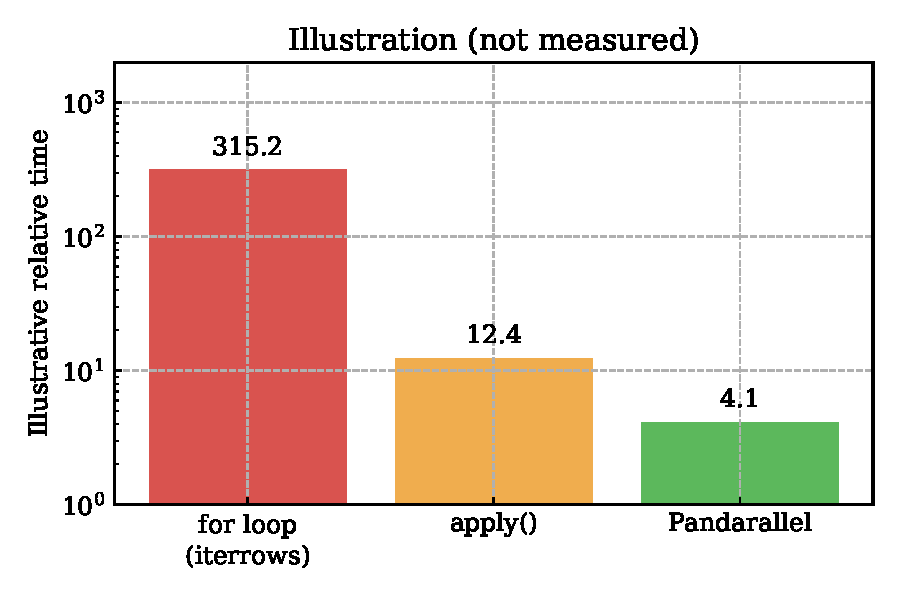
\includegraphics[width=0.7\linewidth]{pandas_benchmark.pdf}
\caption{同じ行単位処理に対する Python のループ、\code{apply()}、\code{pandarallel} の模式的な比較。棒の高さは実測値ではなく、入力サイズや 1 行当たりの計算量によって順位も変わり得る。}
\label{fig:pandas-benchmark}
\end{figure}

\code{pandarallel} は、DataFrame を複数プロセスへ分割し、\code{parallel\_apply()} に渡した関数を各部分へ適用する。プロセスの生成、データの直列化、プロセス間転送の時間も加わるため、対象処理について逐次実行との実行時間とメモリ使用量を測定する。

\code{pandarallel} は複数の Python プロセスを起動するため、OS によってプロセスの開始方法や必要な設定が異なる。Windows で本書の Linux 系コマンドと実行条件をそろえる場合は、第~\ref{chap:shell}~章で説明した WSL を利用できる。

\code{pandarallel} は DataFrame を複数プロセスへ分配するため、プロセスの起動、データの受け渡し、結果の結合にも時間がかかる。単純な加算のように 1 行当たりの処理が短い場合は、この付加時間が計算時間を上回り、逐次処理より遅くなることがある。並列化の採否は、同じ入力に対する逐次処理と並列処理を測定して判断する。

\subsection{欠損値と比較演算を混同しない}

\code{NaN == NaN} は \code{False} であるため、欠損判定には \code{==} ではなく \code{isna()} を用いる。\code{None}、\code{NaN}、\code{NA} の使用可否と表示は列型に依存するので、\code{dtype} と欠損値数を確認する。

\section{観測表の集計と可視化への受け渡し}

観測データの解析では、pandas はしばしば次の流れの中心になる。

\begin{enumerate}
\item \code{read\_csv()} によるテキスト・CSV の読み込み
\item \code{head()} と \code{dtypes} による表構造の確認
\item 必要な列の選択と、欠損値・異常値の整理
\item \code{groupby()} と \code{merge()} による集計・結合
\item Matplotlib への受け渡しと作図
\item \code{to\_latex()} による集計表の書き出し
\end{enumerate}

この流れでは、列名と列型を保ったまま抽出、集計、結合、保存を記述している。観測条件、検出器 ID、run 名、欠損フラグのように型の異なる列を一つの記録として扱う場合は、列ごとに型を持つ DataFrame を利用できる。

一方、CSV の読み込みや集計が実測した待ち時間の主要部分を占める場合は、次章で扱う Polars も候補となる。行数だけで切り替えを決めず、必要な機能、メモリ使用量、処理時間を同じ入力で比較する。

また、pandas の多くの操作は、DataFrame が 1 台の計算機のメモリに収まることを前提とする。ただし、\code{read\_csv(chunksize=...)} を使えば、総和や件数のように部分結果を統合できる処理は全件を同時に保持せずに実行できる。必要な表がメモリに収まらない場合は、列と行を早い段階で絞る、分割集計を使う、Parquet に変換する、次章の Polars やデータベースを使う、という順に処理の性質に合う方法を選ぶ。

基本操作の公式資料として Getting started tutorials~\cite{pandas_tutorials} と 10 minutes to pandas~\cite{pandas_10min} がある。列選択と代入は Indexing~\cite{pandas_indexing}、欠損値処理は Missing data~\cite{pandas_missing}、表の結合は Merge, join, concatenate and compare~\cite{pandas_merging}、時刻列は Time series / date functionality~\cite{pandas_timeseries} に詳しい。本章は、これらの機能を解析手順に沿って再構成した。

\section{章末課題：検出器別の表集計}

次の CSV を \code{events.csv} として保存し、すべての課題の共通入力とせよ。

\begin{lstlisting}[numbers=none, xleftmargin=2\zw, title={events.csv}]
detector,time_ns,signal,valid
A,1000,12.4,true
B,1180,9.8,true
A,1300,15.1,true
B,1510,,false
A,1760,11.0,true
B,2050,13.2,true
\end{lstlisting}

\begin{enumerate}
\item \textbf{読み込み直後の表の検査}。
\code{pd.read\_csv()} で読み、\code{shape}、\code{columns}、\code{dtypes}、\code{head(3)}、\code{isna().sum()} を表示せよ。行数は 6、列数は 4、\code{signal} の欠損数は 1 になる。\code{head(3)} の \code{3} と、\code{isna().sum()} の \code{sum()} がどの方向に集計しているかを説明せよ。

\item \textbf{条件抽出と列追加}。
\code{valid} が真で \code{signal >= 12.0} の行を \code{loc} で抽出し、\code{signal / signal.mean()} を \code{signal\_ratio} 列として追加せよ。抽出行は 3 件になる。複数条件を括弧で囲み、\code{and} ではなく \code{\&} を使う理由を説明せよ。

\item \textbf{検出器別集計と別表の結合}。
\code{groupby("detector")} と \code{agg()} を使い、有効な信号の件数、平均、標準偏差を求めよ。平均は A が約 12.8333、B が 11.5 になる。さらに、A と B の較正係数を持つ DataFrame を作り、\code{merge(..., on="detector", how="left")} で結合せよ。\code{on} と \code{how} の役割を説明せよ。

\item \textbf{一括読み込みと分割読み込みの比較}。
本文の \code{chunksize=2} の方法で件数と平均を求め、一括読み込みから得た結果と \code{pd.testing.assert\_frame\_equal()} または \code{np.allclose()} で一致を確認せよ。チャンク平均の単純平均が一般には誤る理由を、件数が異なる 2 チャンクの例を使って説明せよ。

\item \textbf{再利用可能な形式への保存}。
集計表を CSV と Parquet の両方へ保存し、読み戻して列名と値を確認せよ。\code{index=False} を付けた場合に何が保存されないかを説明し、Parquet の読み込みに追加ライブラリが必要な環境では、表示された例外名も記録せよ。
\end{enumerate}

pandas で表処理の基本と結果の検証方法を確認した後は、同じ処理を別の DataFrame 実装で書くと、設計上の違いが明確になる。次章では、Polars による index 非依存の表処理、列式、遅延実行を扱う。

\chapter{Polars による式ベースの表処理}
\label{chap:polars}

Polars\index{polars@Polars|textbf} は、列指向の DataFrame ライブラリである。pandas と同じく表形式データを扱うが、index を持たず、列に対する処理を式として組み立てる点が異なる。\code{LazyFrame}\index{lazyframe@LazyFrame|textbf} では、式から作った実行計画を評価前に最適化できる。本章では、呼び出し時に結果を返す eager API と、処理を実行計画として蓄積する lazy API を区別し、列変換、集計、結合、入出力を扱う。

\section{式と遅延実行による表処理}

\subsection{index を持たない DataFrame}

Polars の DataFrame は、常に「行番号は整数位置でだけ参照する 2 次元表」である。pandas のような index に意味を持たせないため、\code{reset\_index()} や \code{loc} を前提にした設計にはならない。

\begin{lstlisting}[language=Python]
import polars as pl

df = pl.DataFrame(
    {
        "detector": ["A", "A", "B", "B"],
        "time_ns": [1032, 1188, 1055, 1244],
        "signal": [12.4, 10.1, 14.8, 9.7],
    }
)

print(df)
\end{lstlisting}

このコードを実行すると、Polars の表は次のように表示される。

\begin{lstlisting}[numbers=none, xleftmargin=2\zw]
shape: (4, 3)
+----------+---------+--------+
| detector | time_ns | signal |
| ---      | ---     | ---    |
| str      | i64     | f64    |
+==========+=========+========+
| A        | 1032    | 12.4   |
| A        | 1188    | 10.1   |
| B        | 1055    | 14.8   |
| B        | 1244    | 9.7    |
+----------+---------+--------+
\end{lstlisting}

\code{shape: (4, 3)} は 4 行 3 列であることを示し、各列名の下にはデータ型が表示される。Polars の式は行ラベルではなく列名を参照し、その列に適用する処理を表す。

\subsection{式による列変換}

Polars の中心概念は expression（式）\index{expression@expression|textbf}である。式は、列に対してどの計算を適用するかを表す処理記述であり、その時点の値そのものではない。\code{pl.col("signal")} は \code{signal} 列を参照する式であり、四則演算、比較、集計などと組み合わせられる。

\begin{lstlisting}[language=Python]
expr = pl.col("signal") / pl.col("signal").mean()
print(expr)
\end{lstlisting}

表示されるのは、概ね \code{[(col("signal")) / (col("signal").mean())]} のような式であり、4 行分の数値ではない。実際の値を得るには、\code{df.select(expr.alias("signal\_ratio"))} のように、式を DataFrame の処理へ渡す。\code{alias()} は式の結果へ列名を付ける。Polars の公式ドキュメント~\cite{polars_expressions} でも、expression は列処理を構成する基本概念として説明されている。\code{select()}、\code{with\_columns()}、\code{filter()}、\code{group\_by()} の多くは、式を受け取る API で統一されている。

\subsection{eager と lazy}
\index{polars@Polars!eager api@eager API}
\index{polars@Polars!lazy api@lazy API}

Polars には、命令ごとに結果を返す eager API と、処理を実行計画として蓄え、最後に最適化して実行する lazy API がある。

\begin{lstlisting}[language=Python]
eager_df = pl.read_csv("events.csv")
lazy_df = pl.scan_csv("events.csv")
\end{lstlisting}

\code{read\_csv()} は呼び出し時に読み込んで DataFrame を作るが、\code{scan\_csv()} は実行前の処理計画を表す \code{LazyFrame} を返す。lazy API では、必要な列だけを読む列射影や、不要な行を早い段階で除く述語プッシュダウンなどを適用できる場合がある。処理時間とメモリ使用量への効果は、入力形式と処理内容に依存するため、同じ入力で測定する。

\section{列変換・集計・結合・入出力}

\subsection{\code{select()} と \code{filter()}}

列の選択には \code{select()}\index{select@\code{select}|textbf}、条件に合う行の抽出には \code{filter()}\index{filter@\code{filter}|textbf} を用いる。

\begin{lstlisting}[language=Python]
selected = df.select("detector", "signal")
strong = df.filter(pl.col("signal") > 11.0)

print(selected)
print(strong)
\end{lstlisting}

\code{select()} で列が減り、\code{filter()} で条件に合う行だけが残る。出力は次の通りである。

\begin{lstlisting}[numbers=none, xleftmargin=2\zw]
shape: (4, 2)
+----------+--------+
| detector | signal |
+==========+========+
| A        | 12.4   |
| A        | 10.1   |
| B        | 14.8   |
| B        | 9.7    |
+----------+--------+
shape: (2, 3)
+----------+---------+--------+
| detector | time_ns | signal |
+==========+=========+========+
| A        | 1032    | 12.4   |
| B        | 1055    | 14.8   |
+----------+---------+--------+
\end{lstlisting}

\code{df["signal"]} は列を Series として取り出す。これに対して、\code{select()} や \code{filter()} へ渡した式は、複数列の変換や lazy API の実行計画にも使用できる。値を取り出す操作と、表に適用する式を区別する。

\subsection{\code{with\_columns()} による列の追加}

新しい列は \code{with\_columns()}\index{with_columns@\code{with\_columns}|textbf} で追加する。複数の式を一度に渡すと、それぞれの評価結果が列として追加または置換される。

\begin{lstlisting}[language=Python]
derived = df.with_columns(
    (pl.col("signal") / pl.col("signal").mean()).alias("signal_ratio"),
    (pl.col("time_ns") > 1100).alias("is_late"),
)

print(derived)
\end{lstlisting}

列追加後の表を見ると、式で作った列がどの位置へ入るかを確認できる。

\begin{lstlisting}[numbers=none, xleftmargin=2\zw]
shape: (4, 5)
+----------+---------+--------+--------------+---------+
| detector | time_ns | signal | signal_ratio | is_late |
+==========+=========+========+==============+=========+
| A        | 1032    | 12.4   | 1.055319     | false   |
| A        | 1188    | 10.1   | 0.859574     | true    |
| B        | 1055    | 14.8   | 1.259574     | false   |
| B        | 1244    | 9.7    | 0.825532     | true    |
+----------+---------+--------+--------------+---------+
\end{lstlisting}

\code{alias()} は式の結果へ列名を付ける操作である。式を複数組み合わせる場合は、出力列名を明示すると後続の選択や集計との対応を追いやすい。

\subsection{\code{group\_by()} と集計}

集計も式として書く。\code{group\_by()}\index{group_by@\code{group\_by}|textbf} と \code{agg()} は、pandas の \code{groupby()} に対応する中心的な道具である。

\begin{lstlisting}[language=Python]
summary = (
    derived
    .group_by("detector")
    .agg(
        pl.len().alias("count"),
        pl.col("signal").mean().alias("mean_signal"),
        pl.col("signal").std().alias("std_signal"),
        pl.col("is_late").mean().alias("late_fraction"),
    )
    .sort("detector")
)

print(summary)
\end{lstlisting}

集計後は、検出器ごとに 1 行ずつの表へまとまる。出力は次の通りである。

\begin{lstlisting}[numbers=none, xleftmargin=2\zw]
shape: (2, 5)
+----------+-------+-------------+------------+---------------+
| detector | count | mean_signal | std_signal | late_fraction |
+==========+=======+=============+============+===============+
| A        | 2     | 11.25       | 1.626346   | 0.5           |
| B        | 2     | 12.25       | 3.606245   | 0.5           |
+----------+-------+-------------+------------+---------------+
\end{lstlisting}

Polars の \code{group\_by()} は、集計対象が expression なので、同じ書き方のまま統計量を増やしやすい。\code{count}、\code{mean}、\code{std} のような基本操作は、式の名前を見れば意味を追いやすい。

\subsection{join と表の変形}
\index{polars@Polars!pivot@\code{pivot()}}

別表の較正係数や run 情報を結び付けるなら \code{join()}\index{join@\code{join}|textbf} を使う。縦長と横長の変換も行える。

\begin{lstlisting}[language=Python]
gain = pl.DataFrame(
    {
        "detector": ["A", "B"],
        "gain": [1.02, 0.97],
    }
)

merged = derived.join(gain, on="detector", how="left")
wide = (
    pl.DataFrame(
        {
            "detector": ["A", "A", "B", "B"],
            "kind": ["raw", "cal", "raw", "cal"],
            "value": [12.4, 12.7, 14.8, 14.4],
        }
    )
    .pivot(index="detector", on="kind", values="value")
    .sort("detector")
)

print(merged.select("detector", "signal", "gain"))
print(wide)
\end{lstlisting}

2 つの出力は次のようになる。

\begin{lstlisting}[numbers=none, xleftmargin=2\zw]
shape: (4, 3)
+----------+--------+------+
| detector | signal | gain |
+==========+========+======+
| A        | 12.4   | 1.02 |
| A        | 10.1   | 1.02 |
| B        | 14.8   | 0.97 |
| B        | 9.7    | 0.97 |
+----------+--------+------+
shape: (2, 3)
+----------+------+------+
| detector | raw  | cal  |
+==========+======+======+
| A        | 12.4 | 12.7 |
| B        | 14.8 | 14.4 |
+----------+------+------+
\end{lstlisting}

\code{join()} の \code{on="detector"} は両方の表で照合するキー列を指定し、\code{how="left"} は左側の \code{derived} の全行を残す結合方法を指定する。\code{pivot()} では、\code{index="detector"} が出力表で行を識別する列、\code{on="kind"} が新しい列名になる値、\code{values="value"} がセルへ入る値を表す。Polars には pandas のような index がないため、結合や変形に使う列を引数で明示する。

\subsection{欠損値、\code{null}、\code{NaN}}
\index{polars@Polars!null@\code{null}}
\index{nan@NaN|textbf}

Polars は欠損値の扱いが比較的厳密である。\code{null} と \code{NaN} を区別して考える。

\begin{lstlisting}[language=Python]
missing = pl.DataFrame(
    {
        "signal": [12.4, None, 14.8, float("nan")],
    }
)

print(missing.with_columns(
    pl.col("signal").is_null().alias("is_null"),
    pl.col("signal").is_nan().alias("is_nan"),
))
\end{lstlisting}

判定結果のうち、主要部分は次のようになる。

\begin{lstlisting}[numbers=none, xleftmargin=2\zw]
signal  is_null  is_nan
12.4    false    false
null    true     null
14.8    false    false
NaN     false    true
\end{lstlisting}

\code{null} は値が存在しないこと、\code{NaN} は浮動小数点の特殊値である。\code{is\_nan()} へ \code{null} を渡した結果も \code{null} になる点に注意する。両方を除くなら、例えば \code{pl.col("signal").is\_not\_null() \& pl.col("signal").is\_finite()} をフィルタ条件にする。どちらを落とすかによって使う式が変わる。

\subsection{文字列と条件分岐}

式ベースの API では、文字列処理や条件分岐も列全体に対する式として書く。

\begin{lstlisting}[language=Python]
names = pl.DataFrame(
    {
        "run_name": ["run_A_001", "run_A_002", "test_B_001"],
        "signal": [12.4, 10.1, 14.8],
    }
)

classified = names.with_columns(
    pl.col("run_name").str.extract(r"^(run_[A-Z])", 1).alias("prefix"),
    pl.when(pl.col("signal") > 12.0)
      .then(pl.lit("high"))
      .otherwise(pl.lit("normal"))
      .alias("quality"),
)

print(classified)
\end{lstlisting}

追加した 2 列を含む結果は次の通りである。

\begin{lstlisting}[numbers=none, xleftmargin=2\zw]
run_name    signal  prefix  quality
run_A_001   12.4    run_A   high
run_A_002   10.1    run_A   normal
test_B_001  14.8    null    high
\end{lstlisting}

\code{str.extract()} の第 1 引数は正規表現、第 2 引数の \code{1} は取り出すキャプチャグループの番号である。一致しない \code{test\_B\_001} の \code{prefix} は \code{null} になる。\code{when}、\code{then}、\code{otherwise} は、条件、真の場合の値、偽の場合の値を順に組み立てる。

\subsection{lazy API と \code{scan\_parquet()}}
\index{polars@Polars!scan_parquet@\code{scan\_parquet()}}
\index{polars@Polars!collect@\code{collect()}}

lazy API は、複数の読み込み、抽出、列選択、集計を一つの実行計画として最適化する場合に用いる。

\begin{lstlisting}[language=Python]
lf = (
    pl.scan_parquet("events/*.parquet")
    .filter(pl.col("signal") > 0.0)
    .select("detector", "signal")
    .group_by("detector")
    .agg(pl.col("signal").mean().alias("mean_signal"))
)

result = lf.collect()
print(result)
\end{lstlisting}

\code{scan\_parquet()} の引数 \code{"events/*.parquet"} は、一致する複数の Parquet ファイルを入力にする。戻り値は \code{LazyFrame} であり、この時点ではデータを実体化しない。\code{collect()} を呼ぶとクエリが実行され、戻り値として DataFrame が得られる。実行時には、\code{select()} で使う列だけを読む列射影や、\code{filter()} を早い段階へ移す最適化が適用されることがある。最適化内容を確認したい場合は、実行前に \code{print(lf.explain())} として計画を表示できる。

\subsection{CSV と Parquet の入出力}
\index{polars@Polars!parquet@Parquet}
\index{parquet@Parquet|textbf}

CSV の読み込み、Parquet への保存、遅延読み込みの型の違いを次の例で確認する。

\begin{lstlisting}[language=Python]
df = pl.read_csv("events.csv")
df.write_parquet("events.parquet")

lf = pl.scan_csv("events.csv")
result = lf.filter(pl.col("signal") > 0).collect()

print(type(df).__name__)
print(type(lf).__name__)
print(type(result).__name__)
\end{lstlisting}

表示される型名は順に \code{DataFrame}、\code{LazyFrame}、\code{DataFrame} である。\code{read\_csv()} はその場で読み込み、\code{scan\_csv()} は読み込み計画を作り、\code{collect()} が計画を実行する。\code{write\_parquet()} の第 1 引数は保存先であり、同名のファイルがある場合は上書きされるため、保存先を確認してから実行する。

\code{read\_csv()} と \code{write\_parquet()} は呼び出し時に入出力を行う。\code{scan\_csv()} は \code{LazyFrame} を返し、後続の式を実行計画へ追加する。計画の評価と DataFrame の生成は \code{collect()} が行う。

\section{pandas との違いと遅延実行の注意点}

\subsection{pandas の書き方をそのまま持ち込まない}

Polars と pandas では、同じ DataFrame という名称を使っていても API と実行モデルが異なる。Polars 公式の migration guide~\cite{polars_from_pandas} では、index を前提にせず、列式と処理文脈を用いる設計が説明されている。pandas の \code{loc} や \code{apply(axis=1)} を機械的に置き換えるのではなく、\code{select()}、\code{filter()}、組み込みの式で処理を表現する。

\subsection{\code{map\_elements()} や Python の \code{lambda} を多用しない}
\index{polars@Polars!map_elements@\code{map\_elements()}}

Polars の組み込み式は query optimizer が解析できる。Python の \code{lambda} や \code{map\_elements()} で任意の Python 関数を呼ぶと、最適化や並列実行の範囲が狭まり、呼び出しのオーバーヘッドも加わる場合がある。まず \code{pl.col()}、\code{when}、\code{str}、\code{dt}、\code{over} などの組み込み式で表せるかを確認し、表せない処理にだけ Python 関数を用いる。

\subsection{lazy API では \code{collect()} を忘れない}

\code{scan\_csv()} や \code{scan\_parquet()} は \code{LazyFrame} を返す。\code{print(lf)} が表示するのは実データではなく実行計画である。計画を評価して結果の DataFrame を得るには、\code{collect()} を呼び出す。

\subsection{欠損値における \code{null} と \code{NaN} の区別}

Polars では、各列のデータ型に応じて利用できる式が決まり、値が存在しない \code{null} と浮動小数点値 \code{NaN} は別に扱われる。フィルタや集計の前に列型を確認し、\code{is\_null()} と \code{is\_nan()} のどちらを条件に含めるかを決める。

\section{大規模表処理と可視化への受け渡し}

Polars への移行を検討する条件を次に示す。

\begin{itemize}
\item 複数の CSV または Parquet ファイルに対し、同じ列選択と行抽出を適用する場合
\item 列変換と集計を一つの実行計画として最適化する場合
\item pandas による入出力または集計が、測定した総所要時間の主要部分を占める場合
\item 列射影や述語プッシュダウンを適用できる入力形式と処理内容である場合
\end{itemize}

小規模データで index を用いた対話的操作が必要な場合や、既存コードが pandas の API に依存している場合は、pandas を維持する方が変更量を抑えられる。切り替えの判断には、行数だけでなく、必要な API、移行コスト、メモリ使用量、同じ入力に対する処理時間を用いる。

Polars の概念は Concepts~\cite{polars_concepts}、式は Expressions and contexts~\cite{polars_expressions}、遅延実行は Lazy API~\cite{polars_lazy}、入出力は IO~\cite{polars_io}、pandas との差は Coming from Pandas~\cite{polars_from_pandas} に記載されている。本章は、これらの機能を解析手順に沿って再構成した。

\section{検出器別集計と遅延実行}

共通入力には前章の \code{events.csv} を用いよ。ファイルがない場合は、第~\ref{chap:pandas}~章の章末問題に示した 6 行の CSV を作成せよ。

\begin{enumerate}
\item \textbf{列式による列選択と行抽出}。
\code{pl.read\_csv()} で表を読み、\code{select()} で \code{detector} と \code{signal} だけを選べ。次に、\code{signal} が \code{null} でなく 12.0 以上である行を \code{filter()} せよ。結果は A が 2 行、B が 1 行の計 3 行になる。\code{pl.col()} が値ではなく式を返すことと、\code{is\_not\_null()} を条件に明示する理由を説明せよ。

\item \textbf{列追加と集計を含む単一クエリ}。
\code{with\_columns()} で各検出器の平均からの差 \code{signal\_centered} を作成せよ。この計算には \code{pl.col("signal").mean().over("detector")} を用いよ。その後、\code{group\_by()} と \code{agg()} で件数、平均、最大値を求め、検出器名で並べ替えよ。\code{over("detector")} と \code{group\_by("detector")} の違いを、出力行数に着目して説明せよ。

\item \textbf{lazy API の実行計画と結果の確認}。
\code{pl.scan\_csv("events.csv")} から始め、必要な 2 列の選択、欠損除去、検出器別平均を記述せよ。\code{collect()} の前に \code{explain()} を表示し、その後に \code{collect()} した DataFrame を表示せよ。\code{LazyFrame} と \code{DataFrame} のどちらが実データを保持するかを説明せよ。

\item \textbf{結合と縦横変換}。
検出器と較正係数を持つ表を作り、\code{join(..., on="detector", how="left")} で結合して較正後信号を計算せよ。さらに、検出器を行、\code{valid} を列、件数を値とする表を \code{group\_by()} と \code{pivot()} で作れ。結合キーが重複している場合に出力行数が増える理由も説明せよ。

\item \textbf{pandas との結果照合}。
前章の検出器別集計と同じ統計量を Polars で求め、CSV に保存して pandas で読み戻せ。平均値が一致することを許容誤差付きで確認し、処理速度だけでなく、欠損値、列型、行順序も比較項目になる理由を述べよ。
\end{enumerate}

pandas と Polars で整形・集計した表は、数値を並べただけでは分布、外れ値、変数間の関係を把握しにくい。次章では、それらの列を Matplotlib へ渡し、解析途中の検証図と最終的な説明図を作成する。

\chapter{Matplotlib による可視化}
\label{chap:matplotlib}

Matplotlib\index{matplotlib@Matplotlib|textbf} は、Python でグラフや画像を描画するライブラリである。本章では、データの性質に応じた図の選択と、オブジェクト指向 API による構成要素の制御を扱う。前半では基本的な作図と図種の選択、後半では Figure、Axes、Axis、Artist の関係、複数パネル、スタイル、保存方法を説明する。

ヒストグラム\index{ひすとぐらむ@ヒストグラム}や散布図には、計算結果の検証に用いる診断図としての役割がある。平均値や標準偏差だけでは識別できない長い裾、二峰性、外れ値などを、分布の形として確認できるためである。したがって、解析途中の検証と最終結果の提示の双方に可視化を組み込む。

\section{線図・散布図・ヒストグラムの基本}

\subsection{最小限のヒストグラム}

最初に、乱数生成器のシードを固定して正規乱数を 2500 個生成し、40 個のビンへ数え上げて PDF に保存する。入力は \code{values}、作図処理は \code{plt.hist()}、出力先は \code{histogram.pdf} である。

\begin{lstlisting}[language=Python]
import numpy as np
import matplotlib.pyplot as plt

rng = np.random.default_rng(7)
values = rng.normal(loc=0.0, scale=1.2, size=2500)

plt.hist(values, bins=40)
plt.xlabel("value")
plt.ylabel("count")
plt.savefig("histogram.pdf")
\end{lstlisting}

線、文字、マーカーを主体とする図は、ベクタ形式の PDF で保存すると拡大時にも輪郭を保てる。PDF は LaTeX 文書へ直接挿入できる。図~\ref{fig:basic-histogram-example} は、この最小例の出力である。

\code{plt.show()} は対話的な確認に、\code{savefig()} は出力条件を指定したファイル保存に用いる。保存先、ファイル形式、解像度、同名ファイルを上書きするかどうかを作図コード内で明示すると、図の生成条件を再現できる。

\begin{figure}[tbp]
\centering
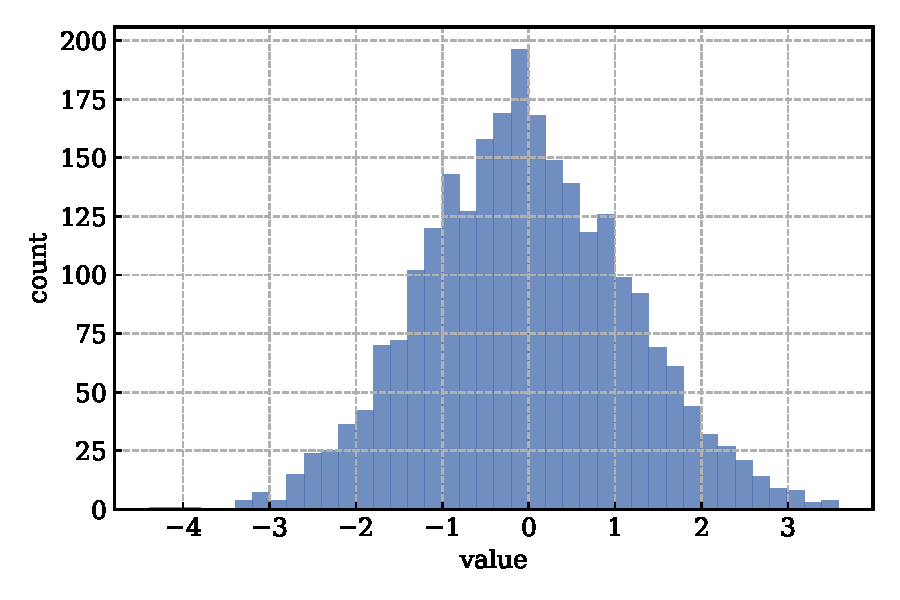
\includegraphics[width=0.72\linewidth]{basic_histogram_example.pdf}
\caption{入力配列 \code{values} を 40 ビンへ数え上げたヒストグラム。横軸は値、縦軸は各ビンに含まれる要素数を表す。}
\label{fig:basic-histogram-example}
\end{figure}

\subsection{軸ラベル、凡例、目盛り}

図には、各軸が表す量と単位、系列を識別する凡例、比較に必要な目盛りを記す。これらが欠けると、数値の物理的意味や系列間の対応を図だけから判定できない。

\begin{lstlisting}[language=Python]
import numpy as np
import matplotlib.pyplot as plt

x = np.linspace(0.0, 10.0, 60)
y = np.exp(-x / 4.0) * (1.0 + 0.08 * np.sin(2.5 * x))

fig, ax = plt.subplots(figsize=(6, 4))
ax.plot(x, y, marker="o", label="sample A")
ax.set_xlabel(r"$t\,[\mathrm{s}]$")
ax.set_ylabel("signal")
ax.set_title("Labeled line example")
ax.set_xticks([0, 2, 4, 6, 8, 10])
ax.legend(loc="upper right")
fig.savefig("labeled_plot_example.pdf")
\end{lstlisting}

図~\ref{fig:labeled-plot-example} には、横軸の量と単位、縦軸の量、系列名、比較に必要な目盛りが示されている。配色を調整する前に、これらの情報が図だけから読み取れるかを確認する。

\begin{figure}[tbp]
\centering
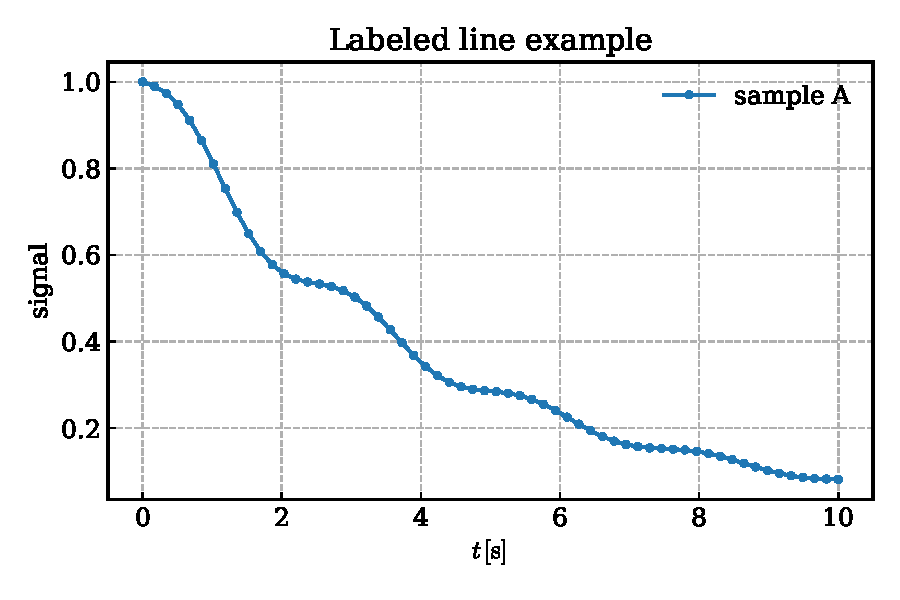
\includegraphics[width=0.72\linewidth]{labeled_plot_example.pdf}
\caption{ラベル、凡例、目盛りを付けた線図。横軸は秒単位の時刻、縦軸は信号値、凡例は系列名を表す。}
\label{fig:labeled-plot-example}
\end{figure}

\subsection{plot 関数へ渡すデータ}

Matplotlib の多くの作図関数は、NumPy 配列や Python リストのような「配列に変換できるもの」を受け取る。加えて、辞書や DataFrame のように列名で参照できるオブジェクトなら、\code{data=} を使って列名指定で描くこともできる。

\begin{lstlisting}[language=Python]
import numpy as np
import matplotlib.pyplot as plt

times = [0, 1, 2, 3]
values = [1.0, 2.0, 1.5, 3.0]

fig, ax = plt.subplots(figsize=(6, 4))
x = np.asarray(times)
y = np.asarray(values)
ax.plot(x, y)

table = {"time": x, "value": y}
ax.plot("time", "value", data=table)
\end{lstlisting}

\code{np.asarray} は、入力を NumPy 配列として扱うことを明示する。\code{data=} を用いる場合は列名を文字列で指定するため、存在しない列名を渡したときのエラーも確認する。独立した配列を渡す場合は、\code{x} と \code{y} を明示する。

\subsection{線・点・参照線・誤差棒の描画関数}

線図には \code{plot()}\index{matplotlib@Matplotlib!plot@\code{plot()}|textbf}、散布図には \code{scatter()}\index{matplotlib@Matplotlib!scatter@\code{scatter()}|textbf}、鉛直および水平の参照線には \code{axvline()}\index{matplotlib@Matplotlib!axvline@\code{axvline()}} と \code{axhline()}\index{matplotlib@Matplotlib!axhline@\code{axhline()}}、誤差付きの点には \code{errorbar()}\index{matplotlib@Matplotlib!errorbar@\code{errorbar()}|textbf} を用いる。次の例は、これらの関数と出力図の対応を示す。

\begin{lstlisting}[language=Python]
import numpy as np
import matplotlib.pyplot as plt

rng = np.random.default_rng(1234)
t = np.linspace(0.0, 10.0, 80)
y = np.sin(t) * np.exp(-t / 12.0)
y_noise = y + 0.12 * rng.normal(size=t.size)
y_err = 0.10 + 0.03 * np.cos(t / 2.0) ** 2

fig, axes = plt.subplots(2, 2, figsize=(10, 7))

axes[0, 0].plot(t, y, marker="o")
axes[0, 1].scatter(t, y_noise, c=t, cmap="viridis")
axes[1, 0].plot(t, y_noise)
axes[1, 0].axvline(3.0, linestyle="--")
axes[1, 0].axhline(0.0, linestyle=":")
axes[1, 1].errorbar(t[::4], y_noise[::4], yerr=y_err[::4], fmt="o")

fig.savefig("basic_plot_types_example.pdf")
\end{lstlisting}

図~\ref{fig:basic-plot-types-example} は、主要な描画関数の出力を並べたものである。線図は順序を持つ系列や関数形、散布図は 2 変量の対応とばらつき、参照線は閾値や基準値、エラーバーは測定値の不確かさを表す。

\begin{figure}[tbp]
\centering
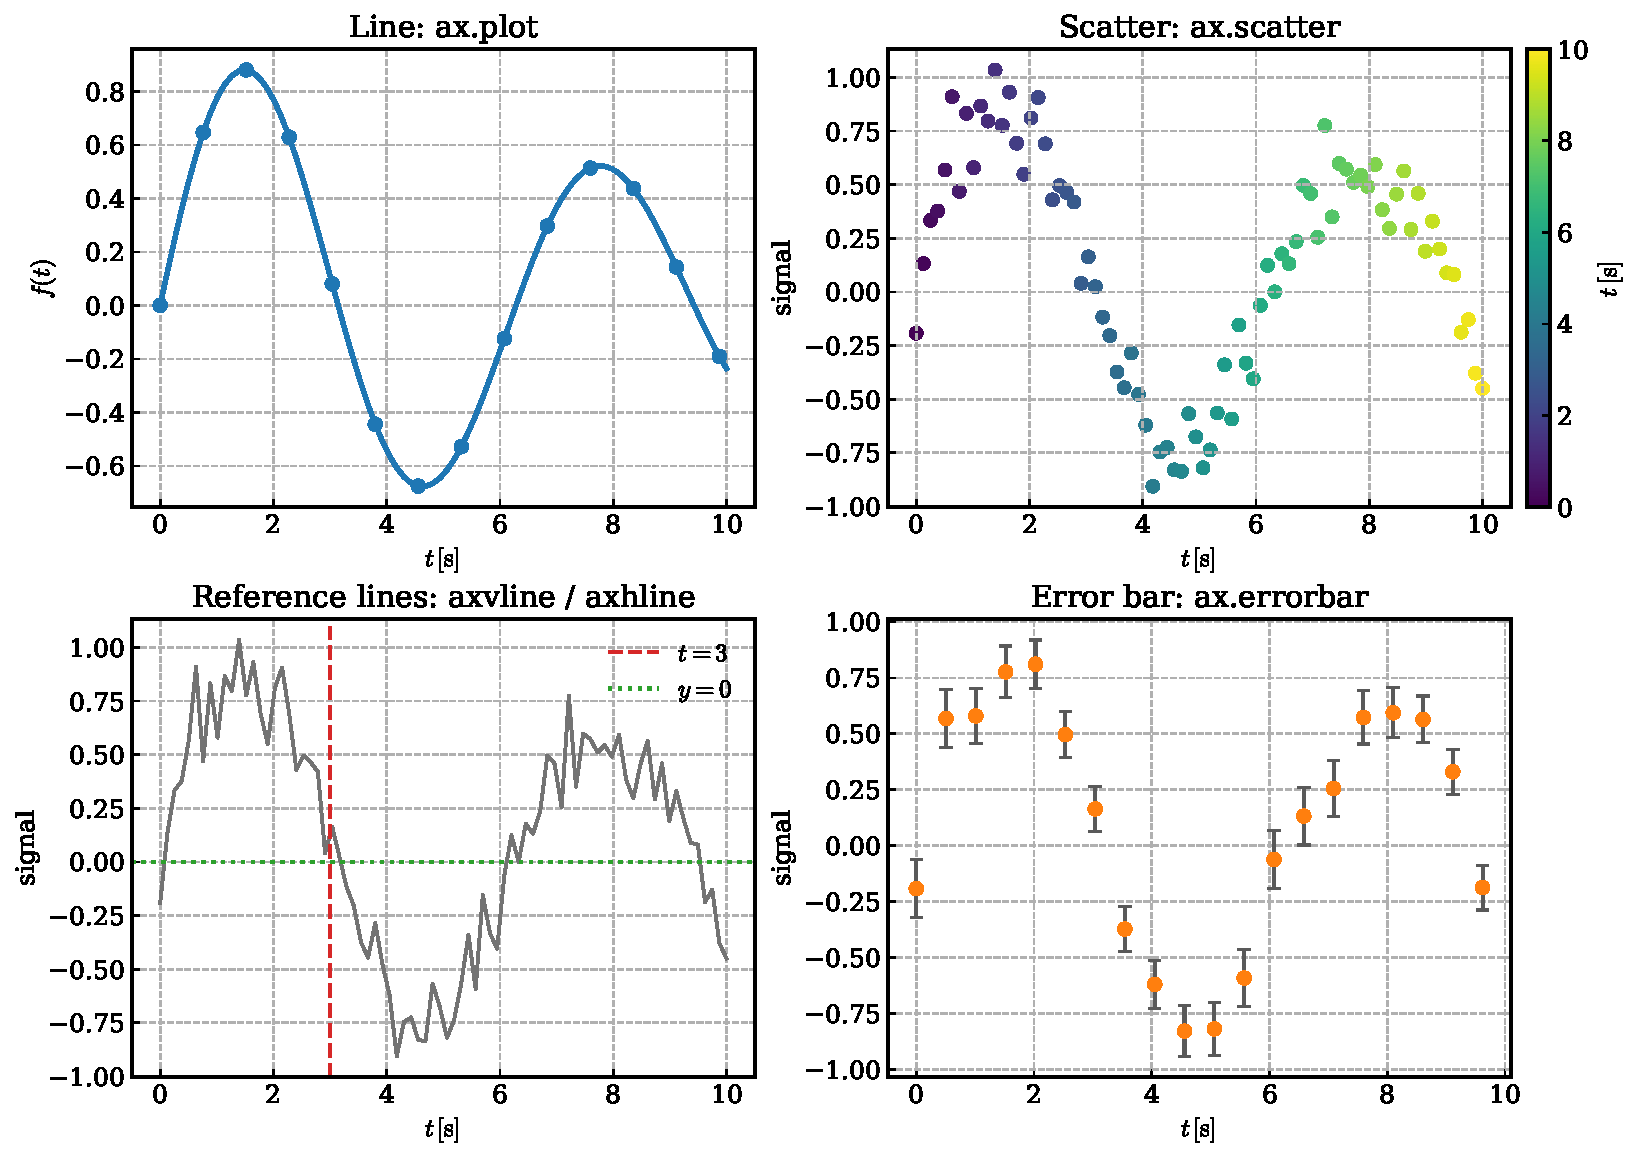
\includegraphics[width=0.94\linewidth]{basic_plot_types_example.pdf}
\caption{主要な描画関数の出力。左上は \code{plot()}、右上は \code{scatter()}、左下は \code{axvline()} と \code{axhline()}、右下は \code{errorbar()} の例である。}
\label{fig:basic-plot-types-example}
\end{figure}

\code{plot()} は既定で点を線で結ぶため、順序を持つ系列または連続関数の表示に用いる。\code{scatter()} は点どうしを結ばず、個々のイベントや標本の 2 変量分布を表示する。\code{axvline()} と \code{axhline()} は、閾値や基準値を対応する軸上へ示す。

\subsection{ヒートマップとカラーバー}

格子上で定義された 2 次元配列は \code{imshow()}\index{matplotlib@Matplotlib!imshow@\code{imshow()}|textbf} で色に対応させる。これに対して、点群を格子ごとに数え上げる場合は \code{hist2d()}\index{matplotlib@Matplotlib!hist2d@\code{hist2d()}|textbf} を用いる。いずれの場合も、色が表す量と尺度をカラーバーに記す。

\begin{lstlisting}[language=Python]
import numpy as np
import matplotlib.pyplot as plt
from matplotlib.colors import LogNorm

x = np.linspace(-3.0, 3.0, 160)
y = np.linspace(-2.5, 2.5, 140)
xx, yy = np.meshgrid(x, y)
image = np.exp(-(xx**2 + 1.6 * yy**2)) + 0.02
rng = np.random.default_rng(1234)
sample_x = rng.normal(loc=0.0, scale=1.0, size=80000)
sample_y = 0.7 * sample_x + rng.normal(loc=0.0, scale=0.8, size=80000)

fig, axes = plt.subplots(1, 2, figsize=(10, 4))
im = axes[0].imshow(image, origin="lower", cmap="viridis", aspect="auto")
fig.colorbar(im, ax=axes[0], label="intensity")

h = axes[1].hist2d(sample_x, sample_y, bins=90, norm=LogNorm(), cmap="magma")
fig.colorbar(h[3], ax=axes[1], label="counts")
\end{lstlisting}

図~\ref{fig:heatmap-colorbar-example} の左は \code{imshow()} によるヒートマップ、右は \code{hist2d()} と \code{LogNorm} を使った 2 次元ヒストグラムである。\code{cmap=} は値から色への対応\index{からーまっぷ@カラーマップ}を定め、\code{fig.colorbar(...)} はその対応尺度と量名を図中に示す。

\begin{figure}[tbp]
\centering
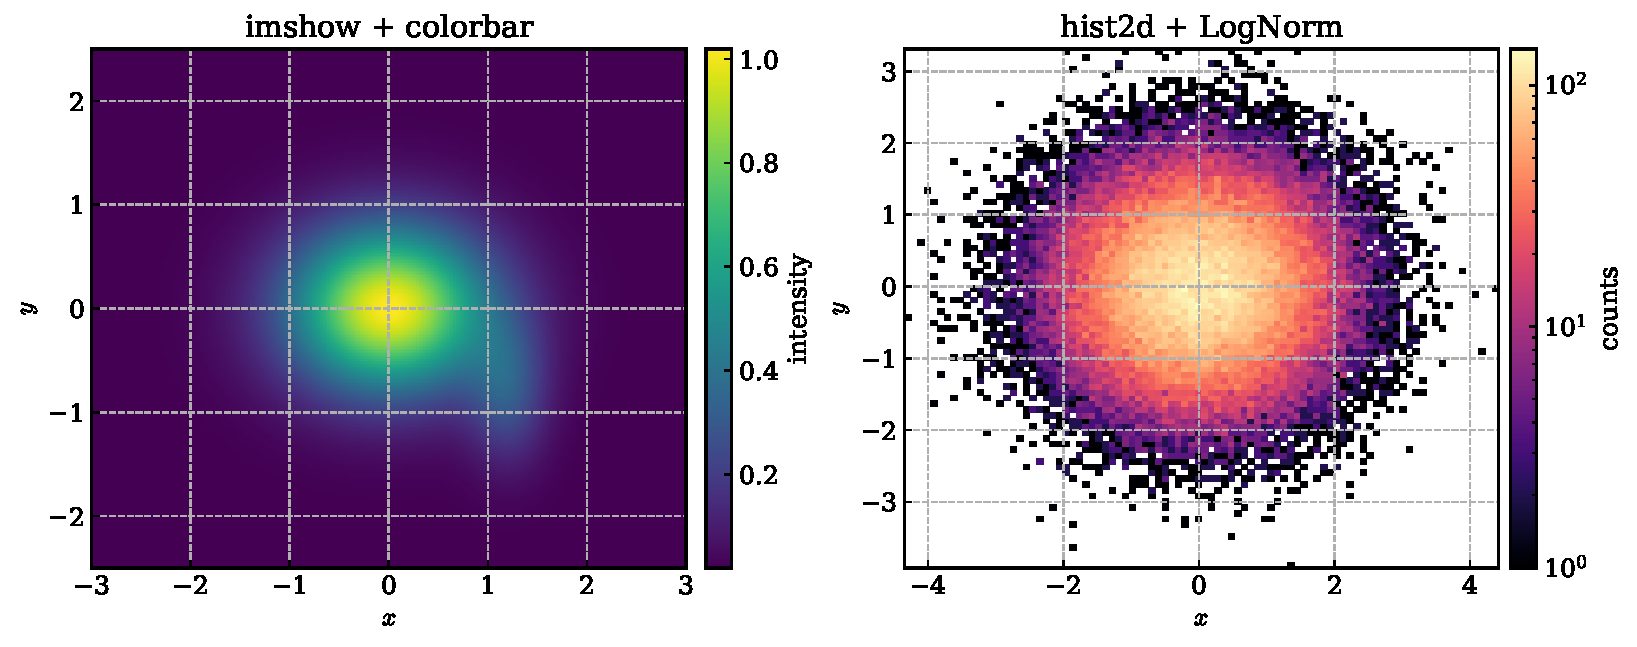
\includegraphics[width=0.94\linewidth]{heatmap_colorbar_example.pdf}
\caption{ヒートマップとカラーバーの例。左は \code{imshow()}、右は \code{hist2d()} と \code{LogNorm} を使った例であり、どちらもカラーバーによって色の意味を示している。}
\label{fig:heatmap-colorbar-example}
\end{figure}

\code{imshow()} は格子上に並んだ値を描くため、シミュレーションで得た場や画像データをそのまま表示できる。一方、\code{hist2d()} は点群を格子ごとに数え上げる。点数が数桁にわたる場合は、\code{LogNorm()} による対数的な色割り当てによって、高密度領域と低密度領域を同じ図に表示できる。

\subsection{全天図と投影: Hammer 図法と Mollweide 図法}

経度と緯度のような球面上のデータを平面へ描くには、投影法\index{とうえいほう@投影法}が必要になる。Matplotlib には、地図ライブラリなしでも使える全天図向けの投影として、Hammer\index{hammer@Hammer projection} 図法や Mollweide\index{mollweide@Mollweide projection} 図法が用意されている。

\begin{lstlisting}[language=Python]
import numpy as np
import matplotlib.pyplot as plt

lon_deg = np.linspace(-180.0, 180.0, 241)
lat_deg = 25.0 * np.sin(np.deg2rad(2.0 * lon_deg))
lon = np.deg2rad(lon_deg)
lat = np.deg2rad(lat_deg)

fig = plt.figure(figsize=(10, 4))
ax1 = fig.add_subplot(1, 2, 1, projection="hammer")
ax2 = fig.add_subplot(1, 2, 2, projection="mollweide")

ax1.scatter(lon, lat)
ax2.scatter(lon, lat)
\end{lstlisting}

図~\ref{fig:projection-examples} は、同じ点群を Hammer 図法と Mollweide 図法で投影した例である。どちらも経度の全範囲と両極を有限の領域に写すため、全天イベント分布や銀河座標図に利用できる。\code{projection="hammer"} と \code{projection="mollweide"} の座標値にはラジアンを渡す。

\begin{figure}[tbp]
\centering
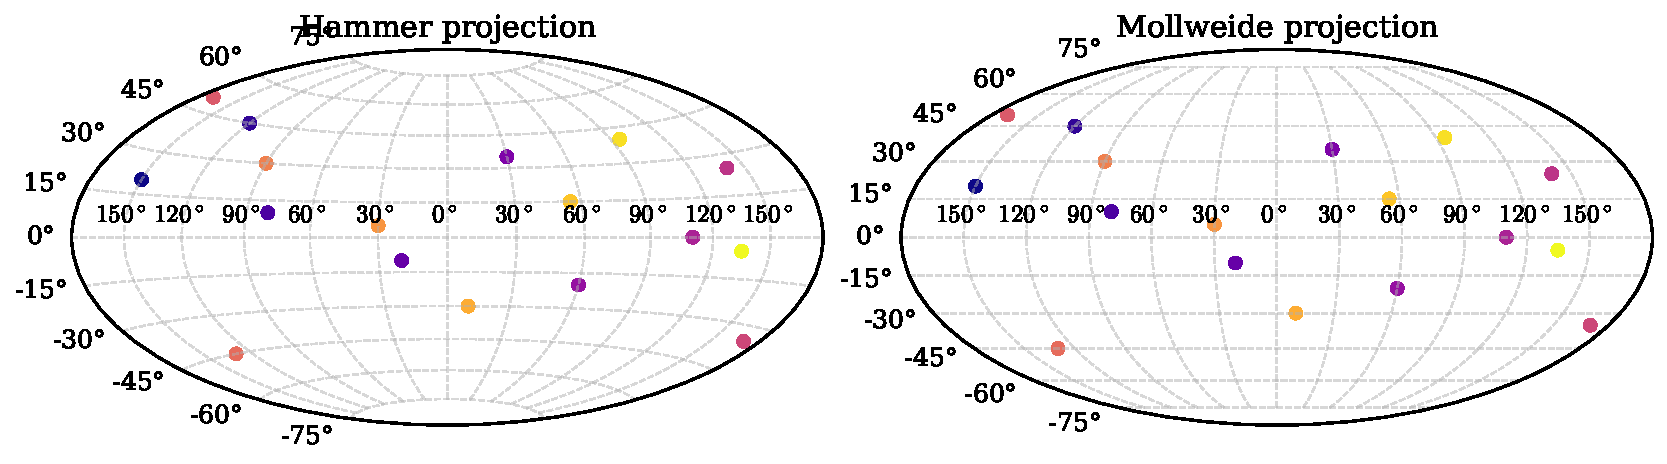
\includegraphics[width=0.94\linewidth]{projection_examples.pdf}
\caption{Hammer 図法と Mollweide 図法の例。どちらも経度の全範囲と両極を一つの楕円領域内に投影する。}
\label{fig:projection-examples}
\end{figure}

国境、海岸線、地理座標系の変換を必要とする地図には Cartopy を用いる。球面座標上の点分布だけを表示する場合は、Matplotlib の標準投影を利用できる。入力座標の単位、経度の範囲、周期境界における処理を作図前に確認する。 Cartopy は追加のライブラリであり、導入方法は公式資料~\cite{cartopy_docs} を参照する。海岸線などの地図データを初めて使う際には取得が必要になる場合がある。


\section{分布・相関・密度に応じた図の選択}

2 変数の関係を調べるときに、データ量を確認せず散布図を描くだけでは、点の重なりによって密度構造を見落とす場合がある。この節の対象は、データ点数と確認したい性質に応じた散布図、透過表示、2 次元ヒストグラムの選択である。

\subsection{度数と確率密度の区別}
\index{ひすとぐらむ@ヒストグラム!せいきか@正規化|textbf}\index{かくりつみつど@確率密度|textbf}
\code{hist()} の既定の縦軸はビン内の度数である。\code{density=True} は、幅 \(\Delta x_i\) のビンの度数 \(n_i\) を \(n_i/(N\Delta x_i)\) に正規化する。ここで \(N\) は表示範囲内で数えた総度数であり、全ビンの面積の和が 1 になる。棒の高さの和が 1 になるとは限らない。

不等幅ビンや対数間隔のビンでは、広いビンほど多くの点が入り得る。分布の形を比較する場合は、度数、単位幅当たりの度数、確率密度のどれを示すかを軸に明記する。\code{density=True} は横軸の値そのものの幅で割る指定であり、対数軸にしただけで対数値の確率密度にはならない。確率密度関数を重ねるときも、正規化する範囲と単位をそろえる。

\subsection{点の重なりに応じた表示方法の選択}

\subsubsection{散布図による点の重なりの確認}

2 変数の対応を点ごとに示す基本的な方法が散布図（\code{scatter}）である。ただし、データ点が多い場合は同じ領域に点が重なり、局所的な密度差を判別できなくなる。

\begin{lstlisting}[language=Python]
import numpy as np
import matplotlib.pyplot as plt

# 約 60 万点を不透明な点として描画する
rng = np.random.default_rng(19)
x = rng.normal(loc=0.0, scale=1.0, size=600_000)
y = 0.65 * x + rng.normal(loc=0.0, scale=0.55, size=x.size)

fig, ax = plt.subplots(figsize=(6, 5))
ax.scatter(x, y, s=10, c='black')
fig.savefig("scatter_bad.png", dpi=150)
\end{lstlisting}

\begin{figure}[htbp]
\centering
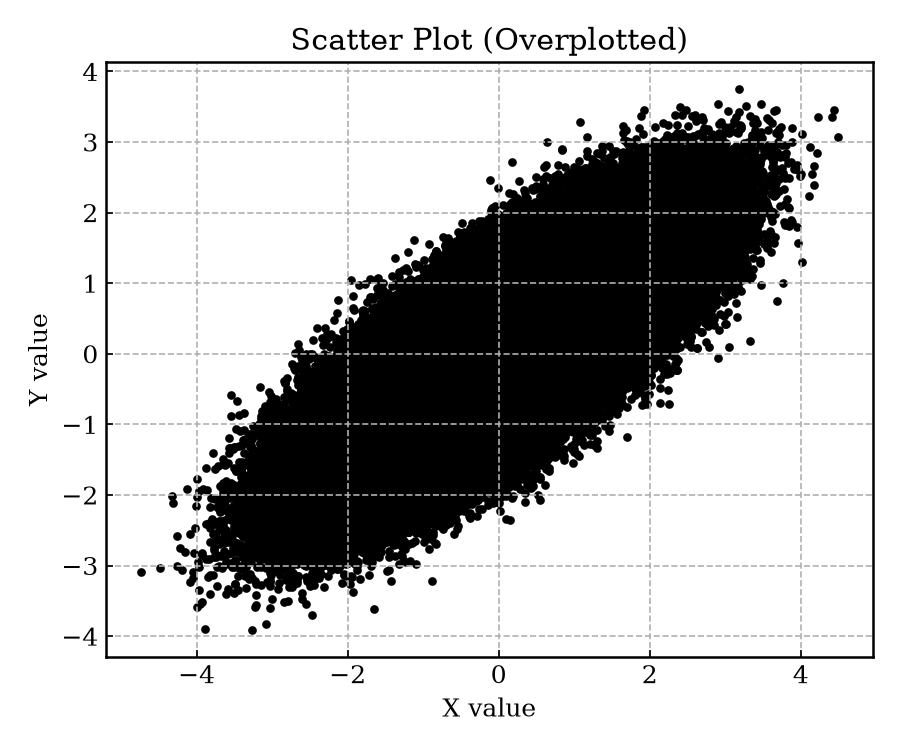
\includegraphics[width=0.6\linewidth]{scatter_bad.png}
\caption{約 60 万点を不透明な点で描いた散布図。点の重なりによって、中心部の密度差を判別できない。}
\label{fig:scatter-bad}
\end{figure}

図~\ref{fig:scatter-bad} からは点が存在する範囲は分かるが、各領域の点数は読み取れない。領域間の密度は、点数をビンごとに集計する 2 次元ヒストグラムで比較する。

\subsubsection{2 次元ヒストグラムによる密度の計数}

2 次元ヒストグラム（\code{hist2d}）は、領域ごとの点数を色で表すため、点の重なりがある場合にも密度を定量的に示せる。

\begin{lstlisting}[language=Python]
fig, ax = plt.subplots(figsize=(6, 5))
h_lin = ax.hist2d(x, y, bins=50, cmap='viridis')
cbar = fig.colorbar(h_lin[3], ax=ax, label="Counts (Linear)")
fig.savefig("hist2d_linear_bad.pdf")
\end{lstlisting}

\begin{figure}[htbp]
\centering
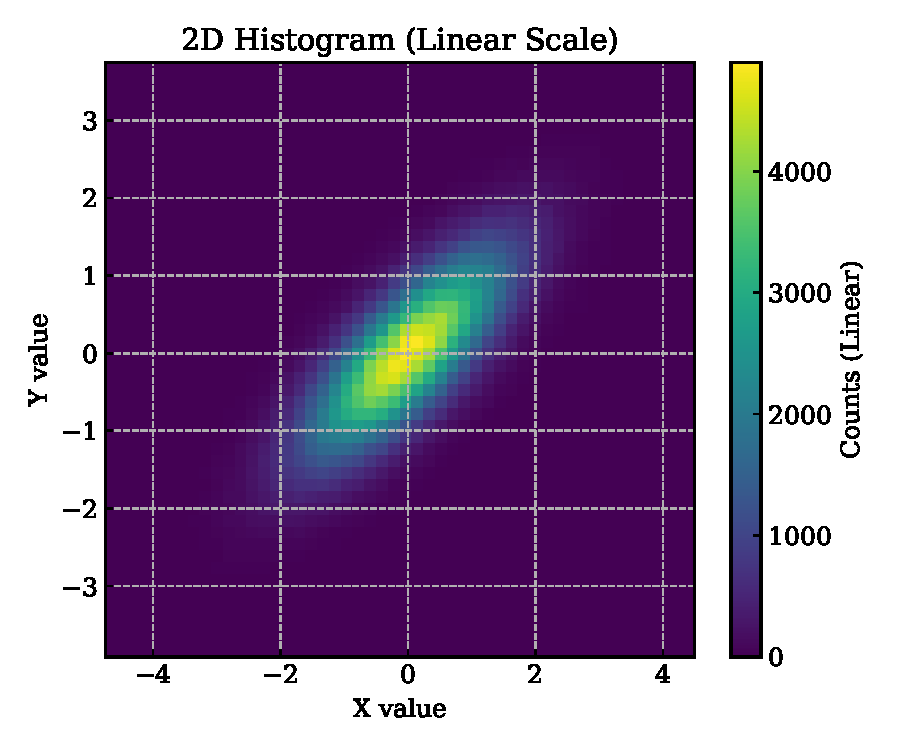
\includegraphics[width=0.6\linewidth]{hist2d_linear_bad.pdf}
\caption{線形カラースケールを用いた 2 次元ヒストグラム。中心部の高密度領域に色範囲の大半が割り当てられ、低密度領域の差を識別しにくい。}
\label{fig:hist2d-linear}
\end{figure}

図~\ref{fig:hist2d-linear} では中心部の密度を読み取れるが、中心部と周辺部の度数が大きく異なるため、周辺の少数カウントの領域には近い色が割り当てられる。この線形カラースケールでは、周辺部の密度差や裾の広がりを識別しにくい。

\subsubsection{\code{LogNorm} による広い密度範囲の表示}

物理イベントの頻度が 1、10、100、1000 のように数桁にわたる場合には、線形カラースケールだけでは低密度領域の差を表しにくい。\code{LogNorm} は、正のカウントを対数尺度で色へ割り当てる。\index{matplotlib@Matplotlib!LogNorm@\code{LogNorm}|textbf}

\begin{lstlisting}[language=Python]
import matplotlib.colors as mcolors

fig, ax = plt.subplots(figsize=(6, 5))
# カウントから色への割り当てを対数尺度にする
h_log = ax.hist2d(x, y, bins=50, norm=mcolors.LogNorm(), cmap='viridis')
cbar = fig.colorbar(h_log[3], ax=ax, label="Counts (Log Scale)")
fig.savefig("hist2d_lognorm_good.pdf")
\end{lstlisting}

\begin{figure}[htbp]
\centering
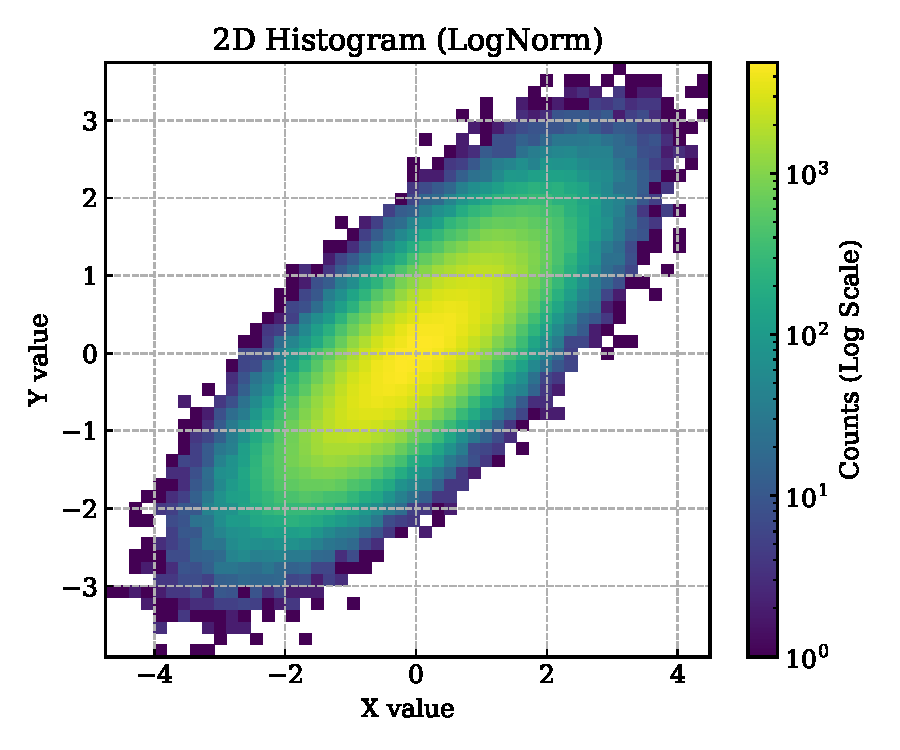
\includegraphics[width=0.6\linewidth]{hist2d_lognorm_good.pdf}
\caption{\code{LogNorm} を用いた 2 次元ヒストグラム。中心の高密度領域と周囲の低密度領域を同じ色尺度で表す。}
\label{fig:hist2d-lognorm}
\end{figure}

図~\ref{fig:hist2d-lognorm}では、単一のピークの周囲に広がる低密度の広がりも判別できる。線形尺度では近い色に対応していた低密度領域が、対数尺度では異なる色に割り当てられるためである。

\subsection{\code{subplots()} による複数パネルの配置}

関連する分布を同じ尺度で比較する場合は、1 枚のキャンバス（\code{Figure}\index{matplotlib@Matplotlib!Figure@\code{Figure}|textbf}）の中に複数のパネル（\code{Axes}\index{matplotlib@Matplotlib!Axes@\code{Axes}|textbf}）を配置する。

\begin{lstlisting}[language=Python]
import numpy as np
import matplotlib.pyplot as plt

rng = np.random.default_rng(23)
data_a = rng.normal(loc=0.0, scale=1.0, size=2000)
data_b = rng.normal(loc=0.4, scale=1.3, size=2000)

# 1 行 2 列（左右に 2 つ）のパネルを作成する。
# fig は Figure 全体、axes は二つの Axes を持つ配列である。
fig, axes = plt.subplots(1, 2, figsize=(10, 4))

# 左のパネルには axes[0] を使って描画する
axes[0].hist(data_a, bins=30)
axes[0].set_title("Data A")

# 右のパネルには axes[1] を使って描画する
axes[1].hist(data_b, bins=30)
axes[1].set_title("Data B")

# 複数のパネルを描くと軸の数字やラベルが隣の図と重なりやすいため、
# 描画後に余白を調整する。
fig.tight_layout()
fig.savefig("histogram_pair_example.pdf")
\end{lstlisting}

複数パネルの図では、\code{axes[0]} のように描画先の \code{Axes} を明示する。これにより、各処理がどのパネルに作用するかをコード上で追跡できる。\code{Figure} と \code{Axes} の役割は、第~\ref{sec:matplotlib-object}~節以降で詳しく説明する。

\subsection{単純な横並び以外: \code{subplot\_mosaic} と \code{GridSpec}}

上段の主結果に広い領域を割り当て、下段に補助図を 2 枚置くなど、パネルごとに面積を変える場合は、\code{subplot\_mosaic()}\index{subplot_mosaic@subplot\_mosaic} または \code{GridSpec}\index{gridspec@GridSpec} を用いる。

\begin{lstlisting}[language=Python]
import numpy as np
import matplotlib.pyplot as plt

values = np.random.default_rng(42).normal(size=2000)
x = np.linspace(0.0, 10.0, 150)
y_top = np.exp(-x / 5.0) * np.cos(2.0 * x)
x_sc = np.linspace(0.0, 1.0, 25)
y_sc = x_sc**2 + 0.05 * np.sin(20.0 * x_sc)

layout = [["A", "A"], ["B", "C"]]
fig, axes = plt.subplot_mosaic(layout, figsize=(10, 6))

axes["A"].plot(x, y_top)
axes["B"].hist(values, bins=40)
axes["C"].scatter(x_sc, y_sc)
\end{lstlisting}

図~\ref{fig:subplot-mosaic-example} のように、\code{"A"} を 2 回書くと、上段の 2 列を一つの Axes が占める。主図と補助図に異なる面積を割り当てる場合に利用できる。

\begin{figure}[tbp]
\centering
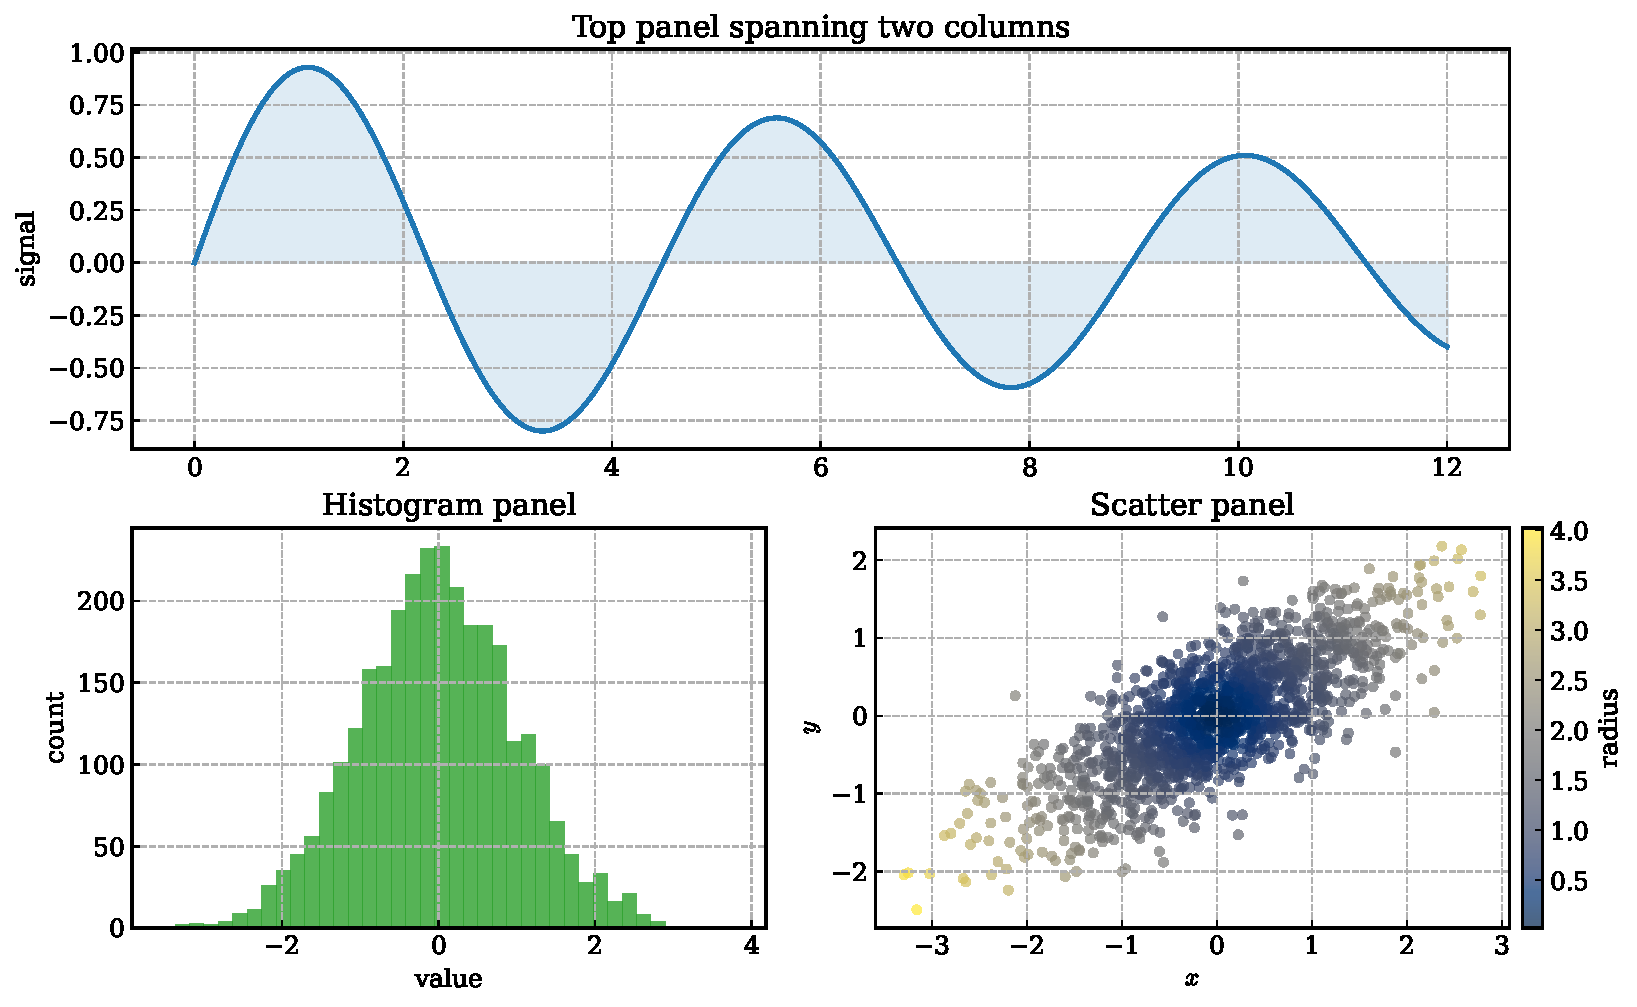
\includegraphics[width=0.92\linewidth]{subplot_mosaic_example.pdf}
\caption{\code{subplot\_mosaic()} を使った複合レイアウトの例。上段は 2 列をまたぐ主図、下段は補助図 2 枚であり、単純な \code{plt.subplots(1, 2)} では作れない配置になっている。}
\label{fig:subplot-mosaic-example}
\end{figure}

\code{subplot\_mosaic()} は文字列の名前で Axes を参照できる。\code{GridSpec} は、列幅、行高、結合するセルを数値で指定する。Axes の参照方法と格子比率の制御範囲に応じて選択する。

\code{LogNorm} は 0 以下の値を対数へ写せないため、空のビンなどは通常マスクされる。背景と同じ色で表示された領域を、微小な正の度数と混同しないようにする。また、\code{imshow()} の既定の座標は画像の画素位置である。物理的な座標で表示する場合は、\code{origin} と \code{extent=(xmin, xmax, ymin, ymax)} で上下の向きと画像の外縁を明示する。

\subsection{凡例とレイアウト}

複数の系列やフィット曲線を同じ図へ重ねる場合は、各系列を識別する凡例が必要である。凡例の位置、枠の有無、項目の順序は、データとの重なりと系列間の対応を考慮して定める。

次の例では、同じ物理量を条件 A と B で測定した状況を正規乱数で模擬する。両パネルに同じビン境界と共有した軸を用い、分布の位置と幅を比較する。

\begin{lstlisting}[language=Python]
import numpy as np
import matplotlib.pyplot as plt

rng = np.random.default_rng(29)
values1 = rng.normal(loc=0.0, scale=1.0, size=3000)
values2 = rng.normal(loc=0.5, scale=1.2, size=3000)

bin_edges = np.linspace(min(values1.min(), values2.min()),
                        max(values1.max(), values2.max()), 41)
fig, axes = plt.subplots(1, 2, figsize=(10, 4), sharex=True, sharey=True)
axes[0].hist(values1, bins=bin_edges, alpha=0.7, label="sample A")
axes[0].set_title("sample A")
axes[0].set_xlabel("value")
axes[0].set_ylabel("count")

axes[1].hist(values2, bins=bin_edges, alpha=0.7, label="sample B")
axes[1].set_title("sample B")
axes[1].set_xlabel("value")

for ax in axes:
    ax.legend(loc="upper right")
    ax.set_axisbelow(True)

fig.tight_layout()
fig.savefig("subplots_example.pdf")
\end{lstlisting}

この例では、\code{axes} は二つの \code{Axes} を並べた配列であり、\code{for ax in axes:} の部分で凡例位置をそろえる処理を両パネルへ適用している。\code{sharey=True} を付けると図~\ref{fig:subplots-example} のように縦軸の尺度がそろうため、左右の高さを直接比較できる。各パネルの系列が一つだけでも凡例を用意しておけば、後からフィット曲線や参照線を追加しても同じ構成を保てる。

\code{tight\_layout} は余白を自動調整するが、すべての文字やパネルの重なりを解消するとは限らない。タイトルや長いラベルが多い場合には、図のサイズや余白を追加で調整する。複数パネルの配置は、比較対象の対応関係が読み取れるかどうかで判断する。

凡例がデータを隠す場合は、\code{loc="best"} で重なりの少ない位置を選ばせるか、\code{bbox\_to\_anchor} で Axes の外側に配置する。自動調整後も、データ、ラベル、凡例の重なりを保存ファイル上で確認する。

\begin{figure}[tbp]
\centering
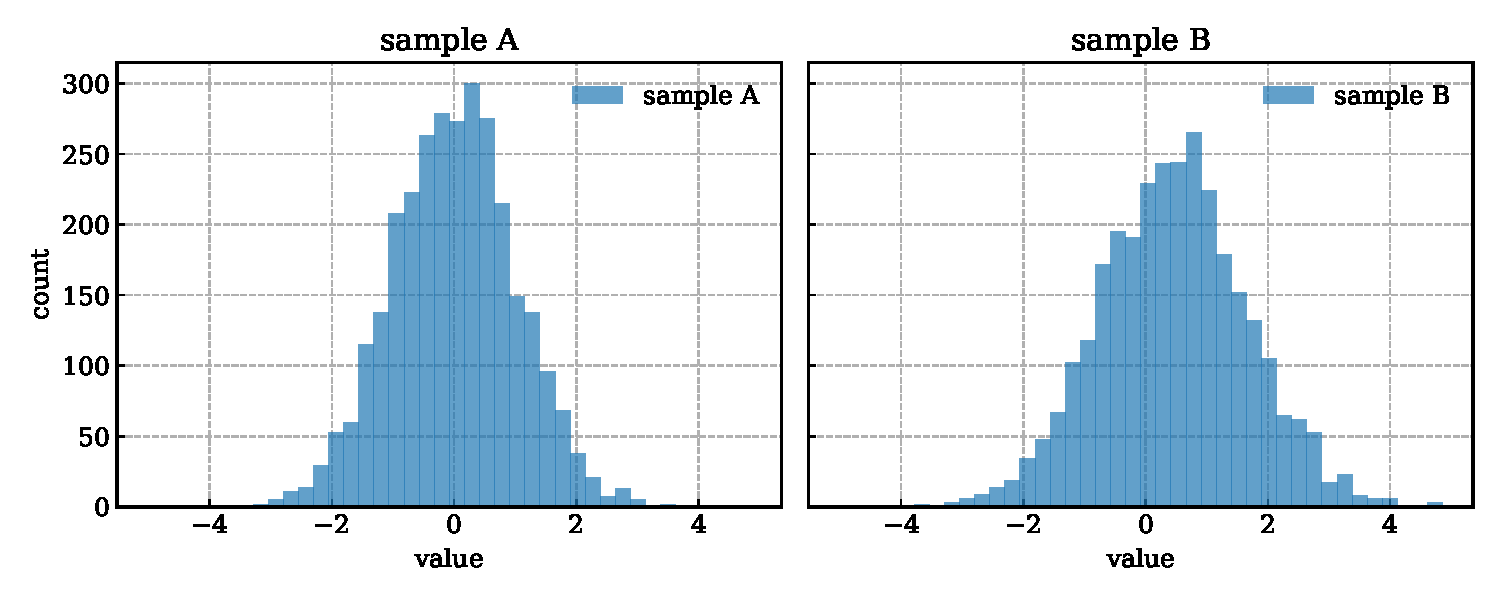
\includegraphics[width=0.92\linewidth]{subplots_example.pdf}
\caption{左右に並べたヒストグラムの出力例。両パネルで縦軸の尺度を共有しているため、同じ高さが同じカウントに対応する。}
\label{fig:subplots-example}
\end{figure}

\subsection{エラーバーと両対数軸}

測定値の不確かさを図に示すには、点とともにエラーバーを描く。値が数桁にわたって変化する場合には、対数軸\index{たいすうじく@対数軸|textbf}を用いると分布形状を比較しやすい。ただし、対数軸では 0 以下の値を表示できないため、データ範囲を事前に確認する必要がある。

図~\ref{fig:errorbar-example} にエラーバーと対数プロットの例を示す。

\begin{figure}[htbp]
\centering
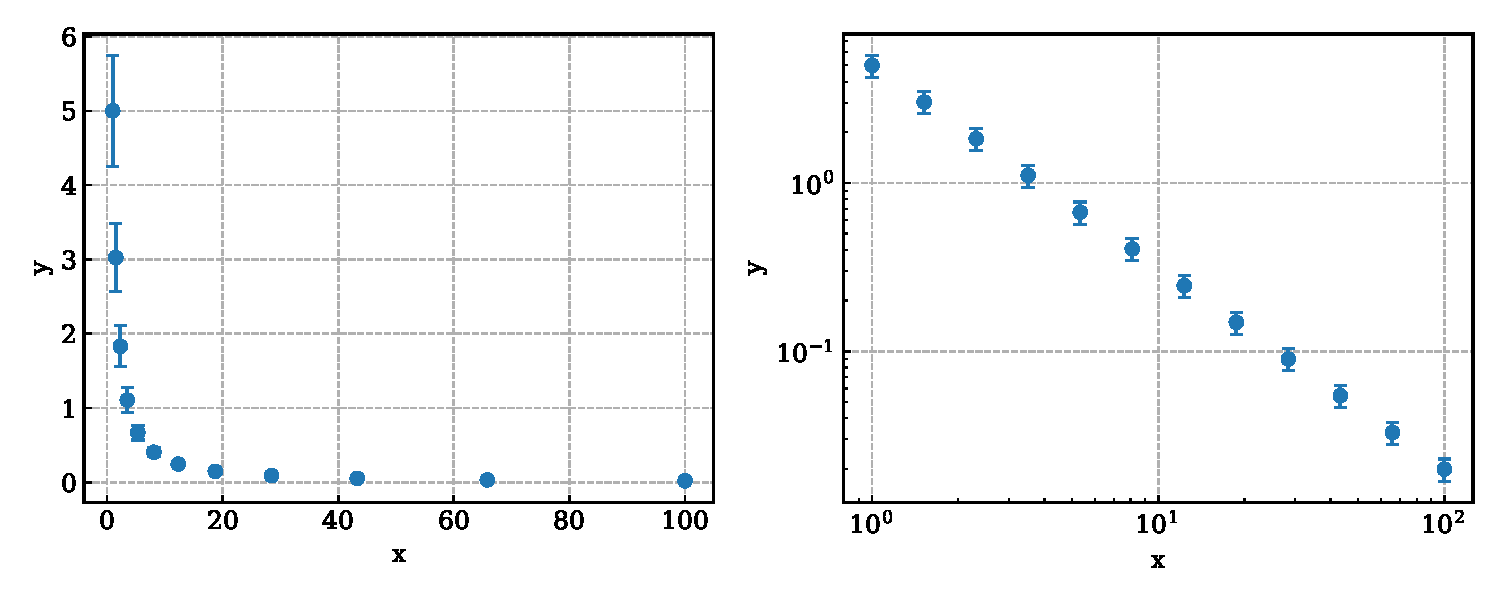
\includegraphics[width=0.92\linewidth]{errorbar_example.pdf}
\caption{エラーバーと対数軸の設定例。左は線形軸、右は x 軸と y 軸の両方を対数尺度にした図。}
\label{fig:errorbar-example}
\end{figure}

\begin{lstlisting}[language=Python]
import numpy as np
import matplotlib.pyplot as plt

x_val = np.geomspace(1.0, 100.0, 12)
y_val = 5.0 * x_val ** (-1.2)
y_err = 0.15 * y_val

fig, axes = plt.subplots(1, 2, figsize=(10, 4))

# fmt='o' は点を丸で描き、capsize=3 は端部の横棒を 3 point にする
axes[0].errorbar(x_val, y_val, yerr=y_err, fmt='o', capsize=3, label="data")
axes[0].set_xlabel("x")
axes[0].set_ylabel("y")

axes[1].errorbar(x_val, y_val, yerr=y_err, fmt='o', capsize=3, label="data")
axes[1].set_yscale('log')
axes[1].set_xscale('log')
axes[1].set_xlabel("x")
axes[1].set_ylabel("y")

fig.tight_layout()
fig.savefig("errorbar_example.pdf")
\end{lstlisting}

\subsection{分布図における軸・色・密度の読み取り}

分布図を解釈するときは、軸が表す量と単位を特定したうえで、分布の中心と幅、裾、外れ値の順に確認する。

例えば、図~\ref{fig:distribution-examples} の左パネルでは、ヒストグラムとフィット曲線の残差、および分布の左右対称性を調べる。右パネルでは、短時間側の立ち上がりと長時間側の減衰を同じ時定数で説明できるかを調べる。本文では、図から読み取った特徴と、その特徴が結論を支える論理を記述する。

\begin{figure}[tbp]
\centering
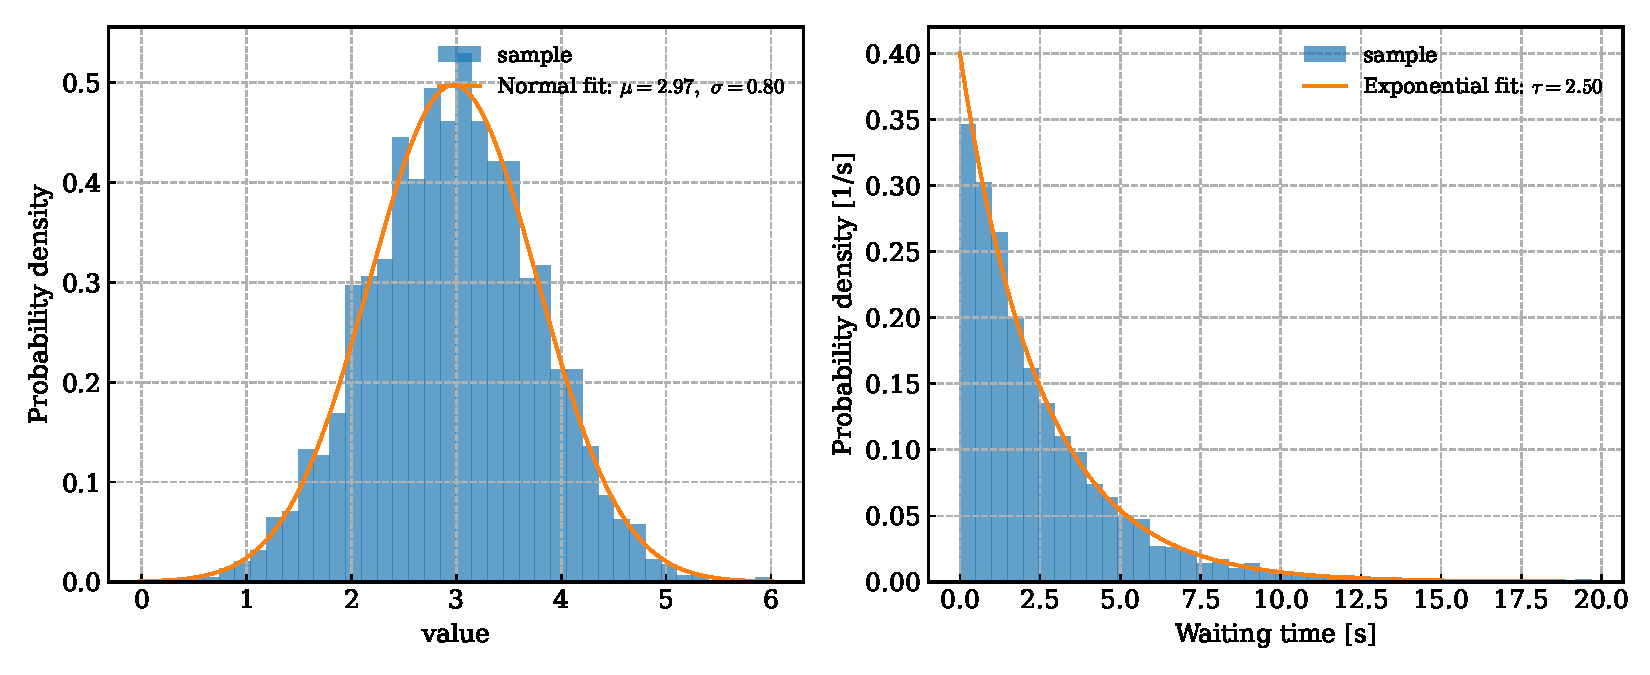
\includegraphics[width=0.92\linewidth]{distribution_examples.pdf}
\caption{Matplotlib による分布図とフィットの例。左はガウシアン型、右は指数分布であり、どちらもヒストグラムの上にフィット曲線を重ね、凡例に分布名と推定パラメータを示している。}
\label{fig:distribution-examples}
\end{figure}

\subsection{画像フォーマットの選択：ラスタとベクタ}\index{matplotlib@Matplotlib!savefig@\code{savefig()}}

解析図の保存形式は、図の要素数、出力先、必要な拡大率に応じて選ぶ。

\begin{itemize}
    \item \textbf{ベクタ形式 (\code{.pdf}, \code{.svg}, \code{.eps})}：線や文字を図形要素として保存するため、拡大しても輪郭がぼやけない。線図や要素数の少ない散布図を論文やレポートへ掲載するときは、\code{savefig("plot.pdf")} のようにベクタ形式で保存する。
    \item \textbf{ラスタ形式 (\code{.png}, \code{.jpg})}：図をピクセルの集合として保存するため、拡大率によっては輪郭に画素が見える。ベクタ形式では各点が個別要素となるので、密集した散布図や各セルを図形として描くヒートマップではファイルサイズと描画負荷が増える。\code{imshow()} の画像は PDF 内にもラスタ画像として埋め込まれる。多数の点やセルだけに \code{rasterized=True} を指定すれば、文字をベクタのまま残すこともできる。図全体を画像にする場合は、\code{savefig("plot.png", dpi=150)} のように必要な解像度を指定して PNG で保存する。
\end{itemize}

\begin{lstlisting}[language=Python]
fig, ax = plt.subplots(figsize=(6, 4))
ax.plot(x, y)
ax.set_xlabel("time [ns]")
ax.set_ylabel("count")

fig.savefig("spectrum.pdf")
fig.savefig("spectrum.png", dpi=150)
\end{lstlisting}

同じ図でも、\code{spectrum.pdf} は線と文字をベクタ要素として保持し、\code{spectrum.png} は指定した画素数のラスタ画像として保存する。線図や要素数の少ないヒストグラムには PDF を用いる。点や格子の数が多く、ベクタ形式ではファイルサイズと描画負荷が増える散布図やヒートマップには、必要な解像度を指定した PNG を用いる。


\section{オブジェクト指向 API による複雑な図の管理}\label{sec:matplotlib-object}

\subsection{Figure, Axes, Axis, Artist の役割}

Matplotlib では、\code{Figure}、\code{Axes}、\code{Axis} が異なる階層を表す。\code{Axes} は複数形に見えるが、Matplotlib では一つの作図領域を表すクラス名である。各オブジェクトの対応を次に示す。

\begin{description}
\item[\code{Figure}] 図全体である。1 つの PDF や PNG、1 つの表示ウィンドウに相当する。\code{savefig}、\code{suptitle}、図全体の凡例や colorbar などは Figure のメソッドまたは構成要素である。
\item[\code{Axes}] データを描く 1 つのパネルである。\code{plot}、\code{hist}、\code{scatter}、\code{set\_xlabel}、\code{legend} などは Axes のメソッドとして呼び出す。
\item[\code{Axis} (\code{x Axis, y Axis})] 目盛り、目盛りラベル、スケールを管理する部品である。通常は \code{ax.set\_xscale("log")} や \code{ax.set\_xlim(...)} のように Axes 経由で触るが、内部には \code{ax.xaxis} と \code{ax.yaxis} がある。
\item[\code{Artist}] 図の中に描かれる要素の総称である。線は \code{Line2D}、文字は \code{Text}、凡例は \code{Legend}、ヒストグラムの棒は \code{Rectangle} という Artist として管理される。代表的な要素を次に示す。
  \begin{itemize}
    \item \code{Title}, \code{Legend}: 図のタイトル、および各系列を示す凡例。
    \item \code{Grid}, \code{Spine}: グリッド線と、座標系を囲む枠線。
    \item \code{Line}, \code{Markers}: 折れ線や散布図の点。
    \item \code{xlabel}, \code{ylabel}: x軸・y軸のラベル。
  \end{itemize}
\end{description}

Figure、Axes、Axis、Artist の階層関係だけを先に図解の構図に合わせて木構造で書くと、次のようになる。

\begin{lstlisting}[numbers=none, xleftmargin=2\zw]
Figure
|-- Axes
|   |-- Title
|   |-- Spine, Grid
|   |-- xaxis, yaxis (x Axis, y Axis / xlabel, ylabel)
|   |-- Line2D, Markers
|   `-- Legend
`-- Figure-level Text / Colorbar / ...
\end{lstlisting}

図~\ref{fig:anatomy-example} に、Figure、Axes、Axis、Artist の位置関係を示す。Figure は一つ以上の Axes を持ち、各 Axes は x 軸と y 軸を表す Axis、および線、文字、凡例などを持つ。Figure、Axes、Axis 自体も Artist の一種であり、四者が互いに独立した分類というわけではない。

\begin{figure}[tbp]
\centering
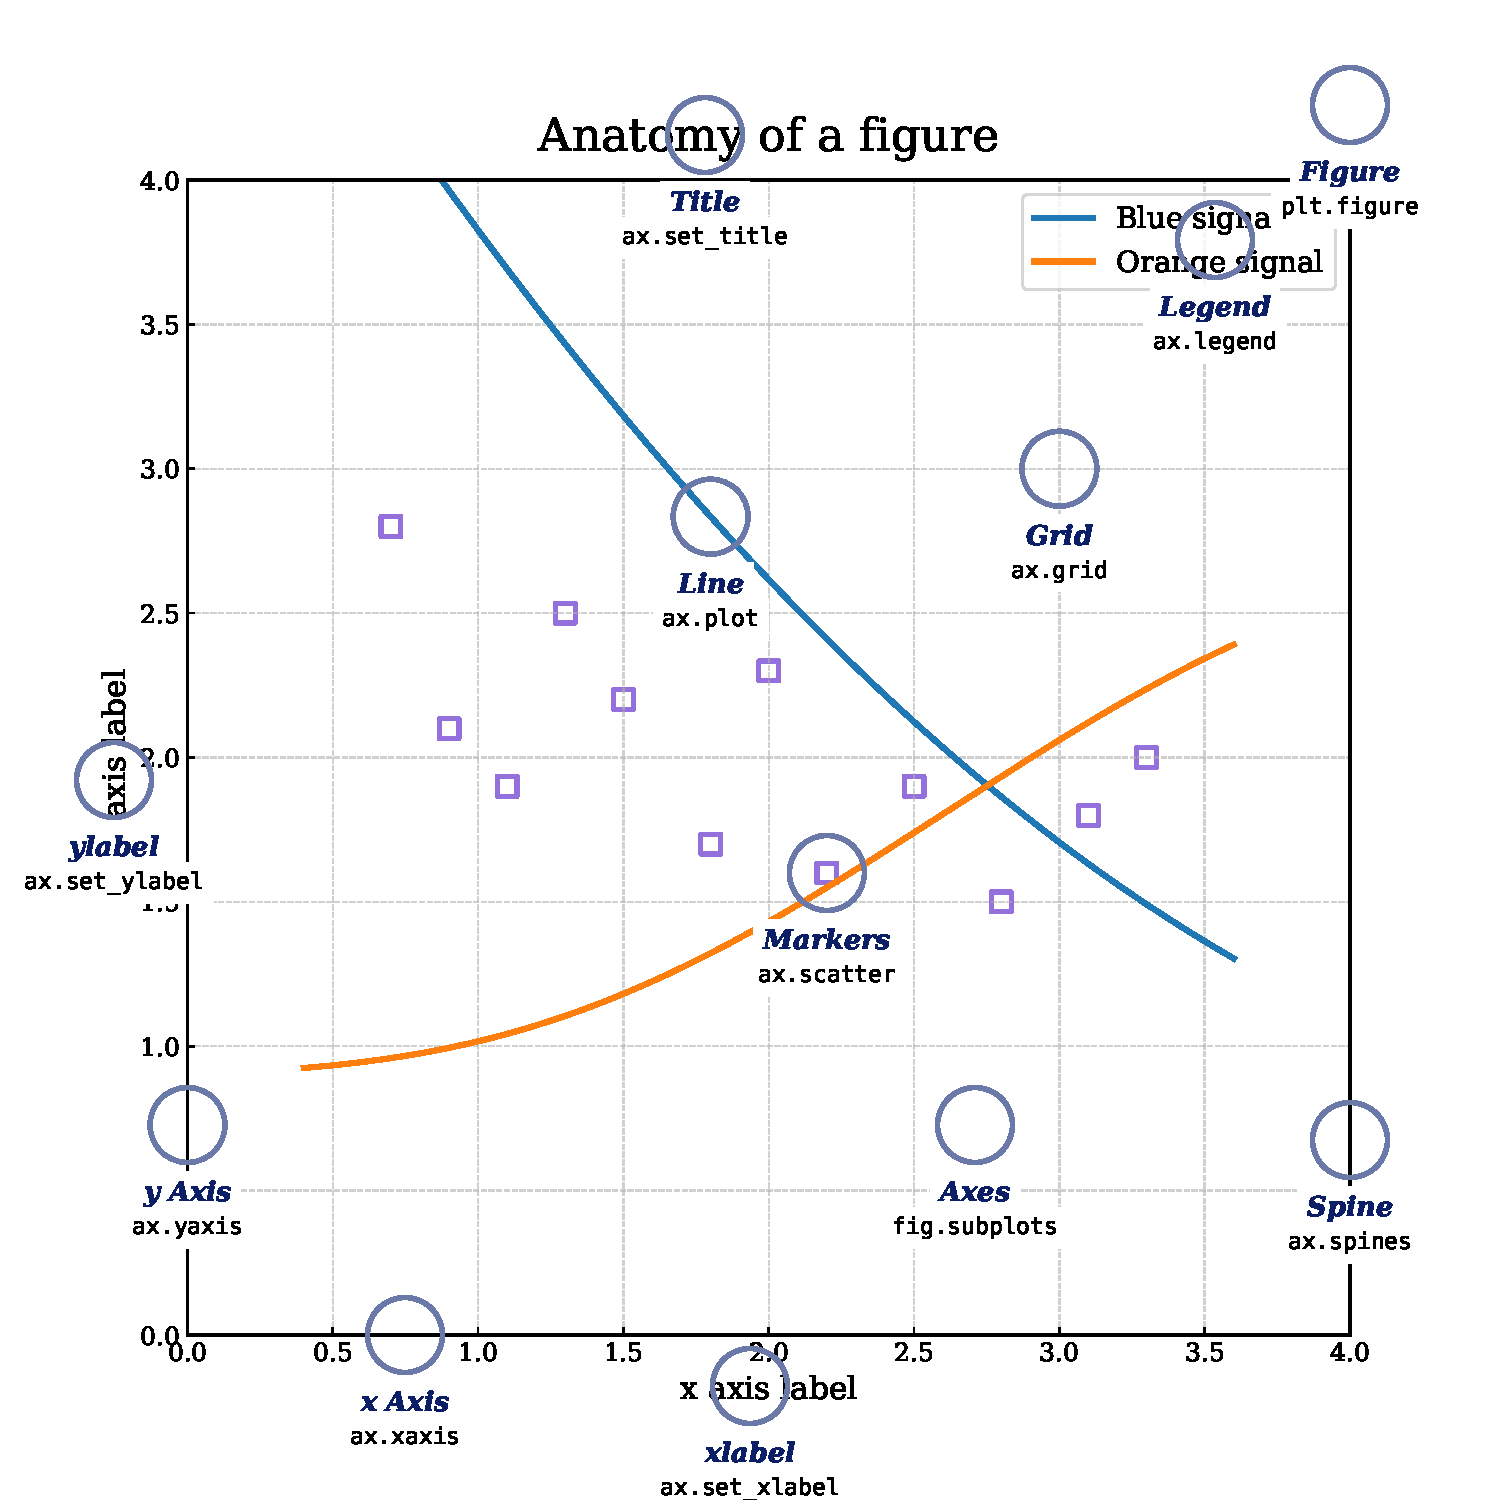
\includegraphics[width=0.75\linewidth]{anatomy_example.pdf}
\caption{Figure、Axes、Axis、Artist の関係を示した例。1 つの Figure の中に Axes があり、その Axes の中で線、文字、凡例などの Artist が描かれている。}
\label{fig:anatomy-example}
\end{figure}

\noindent この対応を実際の Python オブジェクトの型で示すコードを次に掲げる。

\begin{lstlisting}[language=Python]
import matplotlib.pyplot as plt

x = [0, 1, 2, 3]
y = [1.0, 2.0, 1.5, 3.0]

fig, ax = plt.subplots(figsize=(6, 4))
line, = ax.plot(x, y, label="signal")
ax.set_title("Axes title")
ax.set_xlabel("time")
ax.set_ylabel("signal")
legend = ax.legend()

print(type(fig).__name__)
print(type(ax).__name__)
print(type(ax.xaxis).__name__)
print(type(line).__name__)
print(type(legend).__name__)
print(len(fig.axes))
fig.savefig("line.pdf")
\end{lstlisting}

このコードを実行すると、次の出力が得られる。

\begin{lstlisting}[numbers=none, xleftmargin=2\zw]
Figure
Axes
XAxis
Line2D
Legend
1
\end{lstlisting}

最後の \code{1} は、この Figure の中に Axes が 1 枚だけ入っていることを表す。もし \code{plt.subplots(2, 2)} と書けば、Figure は 1 つのままで、Axes が 4 枚入る。

\code{Artist} は線だけを指す名称ではない。タイトルや軸ラベルは \code{Text}、ヒストグラムの各棒は \code{Rectangle} として管理される。次のコードは、それぞれの返り値の型を表示する。

\begin{lstlisting}[language=Python]
import matplotlib.pyplot as plt

fig, ax = plt.subplots(figsize=(6, 4))
title = ax.set_title("Histogram")
xlabel = ax.set_xlabel("value")
bars = ax.hist([1, 1, 2, 3], bins=[0.5, 1.5, 2.5, 3.5])[2]

print(type(title).__name__)
print(type(xlabel).__name__)
print(type(bars).__name__)
print(type(bars[0]).__name__)
\end{lstlisting}

\noindent このコードの出力は次のとおりである。

\begin{lstlisting}[numbers=none, xleftmargin=2\zw]
Text
Text
BarContainer
Rectangle
\end{lstlisting}

ここで \code{bars} 全体は \code{BarContainer} であり、その中の 1 本 1 本は \code{Rectangle} である。したがって、「ヒストグラムの棒だけ色を変える」といった細かい調整は、最終的には Artist を触る操作だと理解できる。

Figure 側の要素も、コード上の型を見ると役割を区別しやすい。図全体タイトル \code{suptitle} や colorbar は、特定の Axes だけでなく Figure 全体の構成に関わる。次のコードは、これらの型を表示する。

\begin{lstlisting}[language=Python]
import numpy as np
import matplotlib.pyplot as plt

fig, ax = plt.subplots(figsize=(5, 4))
img = ax.imshow(np.arange(4).reshape(2, 2))
suptitle = fig.suptitle("Figure title")
cbar = fig.colorbar(img, ax=ax)

print(type(suptitle).__name__)
print(type(cbar).__name__)
\end{lstlisting}

\noindent このコードでは、次の出力が得られる。

\begin{lstlisting}[numbers=none, xleftmargin=2\zw]
Text
Colorbar
\end{lstlisting}

\code{suptitle} は Figure 全体に付く \code{Text} であり、\code{colorbar} は Figure に追加される補助要素である。複数パネルに共通するタイトルや colorbar は、Figure のメソッドを通じて追加する。

Axis は目盛り、目盛りラベル、表示範囲、尺度を管理する。次の操作は、Axes のメソッドを通じて x Axis の設定を変更する。

\begin{lstlisting}[language=Python]
fig, ax = plt.subplots(figsize=(6, 4))
ax.plot([1, 10, 100], [2, 3, 5], marker="o")
ax.set_xlim(1, 100)
ax.set_xscale("log")
\end{lstlisting}

\code{set\_xlim} は表示範囲を、\code{set\_xscale("log")} は座標値から表示位置への変換を対数尺度へ変更する。多くの設定は、\code{ax.xaxis} を直接操作せず、Axes のメソッドから変更できる。

操作対象とメソッドの対応を次に示す。

\begin{itemize}
\item 図全体を保存する、図全体タイトルを付ける: Figure
\item 線やヒストグラムを描く、軸ラベルや凡例を付ける: Axes
\item 対数軸、目盛り位置、目盛りラベルを変える: Axis 関連。ただし実際の操作は Axes メソッド経由が多い
\item 特定の線だけ色や太さを変える、凡例や文字を細かく調整する: Artist
\end{itemize}

保存には \code{fig.savefig(...)}、凡例には \code{ax.legend()}、対数軸には \code{ax.set\_xscale("log")} を用いるのは、それぞれの操作対象が Figure または Axes だからである。各メソッドの呼び出し元が \code{fig} と \code{ax} のどちらかを追うと、処理対象を判別しやすい。

\subsection{オブジェクト指向 API による描画}

Matplotlib には、現在の作図状態へ描画する \code{pyplot} API と、\code{Figure} と \code{Axes} を明示的に操作するオブジェクト指向 API がある。複数パネルや再利用する作図関数では、描画先を引数として渡せる後者を用いる。

\begin{lstlisting}[language=Python]
import numpy as np
import matplotlib.pyplot as plt

rng = np.random.default_rng(7)
values = rng.normal(loc=0.0, scale=1.2, size=2500)

fig, ax = plt.subplots(figsize=(6, 4))
ax.hist(values, bins=40)
ax.set_xlabel("value")
ax.set_ylabel("count")
fig.savefig("histogram.pdf")
\end{lstlisting}

描画先の \code{ax} を明示すると、同じ処理を複数の Figure や Axes に適用できる。また、関数の引数として Axes を受け取れるため、作図処理を再利用できる。

\code{Figure} と \code{Axes} の区別は、設定の適用範囲にも対応する。図全体のタイトルや余白は Figure、軸ラベルや凡例は各 Axes に設定する。

\subsection{補助関数による作図処理の集約}

同じ体裁の図を反復して作成する場合は、Axes を引数に取る補助関数へ作図処理をまとめる。

\begin{lstlisting}[language=Python]
import numpy as np
import matplotlib.pyplot as plt

def plot_hist(ax, values, label):
    ax.hist(values, bins=40, alpha=0.7, label=label)
    ax.set_xlabel("value")
    ax.set_ylabel("count")
    ax.legend(loc="upper right")

rng = np.random.default_rng(0)
values1 = rng.normal(loc=0.0, scale=1.0, size=2500)
values2 = rng.normal(loc=0.8, scale=1.3, size=2500)

bin_edges = np.linspace(min(values1.min(), values2.min()),
                        max(values1.max(), values2.max()), 41)
fig, axes = plt.subplots(1, 2, figsize=(10, 4), sharex=True, sharey=True)
plot_hist(axes[0], values1, "sample A")
plot_hist(axes[1], values2, "sample B")
fig.savefig("histogram_pair_helper.pdf")
\end{lstlisting}

この補助関数は描画先の Axes を引数として受け取るため、比較図の各パネルや条件ごとの反復描画に同じ処理を適用できる。

\section{ラベル・凡例・色・スタイルの管理}

図の可読性に関わる主な要素は次のとおりである。

\begin{itemize}
\item 量と単位を含む軸ラベル
\item 簡潔なタイトル
\item 適切な余白
\item 統一された色と線幅
\item レポート全体で一貫した表記
\end{itemize}

色、フォント、線幅、軸ラベル、単位、凡例の規則を文書全体で統一すると、同じ表現が同じ意味に対応する。系列や条件の区別には、文書内で一貫した色、マーカー、線種を割り当てる。

\subsection{マーカー、線種、色の指定}

Matplotlib では、点の形\index{marker@marker}、線種\index{linestyle@linestyle}、色をそれぞれ独立に指定できる。対応する主な引数は次の 5 つである。

\begin{lstlisting}[language=Python]
ax.plot(
    x,
    y,
    marker="o",
    markersize=5,
    linestyle="--",
    linewidth=2.0,
    color="C3",
)
\end{lstlisting}

\begin{itemize}
\item \code{marker}: 点の形を決める。
\item \code{markersize}: 点の大きさを point 単位で指定する。\code{scatter()} の \code{s} は point の二乗単位であり、同じ数値でも意味が異なる。
\item \code{linewidth}: 線の太さを point 単位で指定する。
\item \code{linestyle}: 実線、破線、点線などを決める。
\item \code{color}: 線や点の色を決める。
\end{itemize}

図~\ref{fig:style-reference-example} は、マーカー、線種、既定の色循環の指定と描画結果を並べたものである。

\begin{figure}[tbp]
\centering
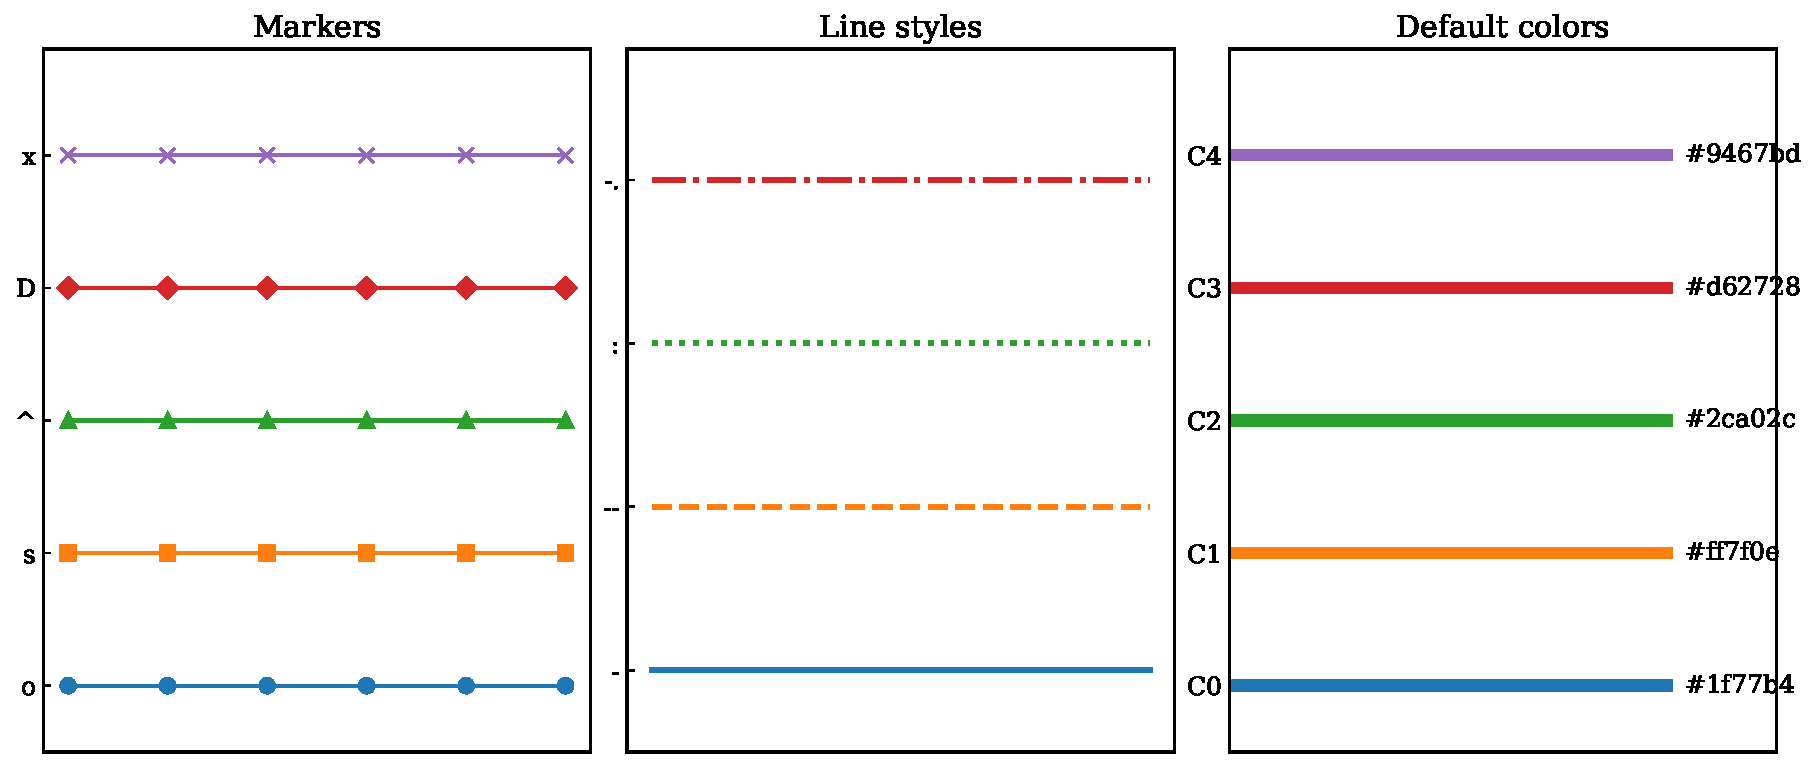
\includegraphics[width=0.92\linewidth]{style_reference_example.pdf}
\caption{マーカー、線種、既定色の代表例。各指定と描画結果の対応を示す。}
\label{fig:style-reference-example}
\end{figure}

図~\ref{fig:style-reference-example} では、マーカー、線種、色の各指定と描画結果を比較できる。個々の指定と用途は、マーカーを表~\ref{tab:matplotlib-markers}、線種を表~\ref{tab:matplotlib-linestyles}、色を表~\ref{tab:matplotlib-colors} にまとめた。系列の識別を色だけに依存させず、マーカーまたは線種も併用すれば、白黒印刷でも系列間の差を保持できる。

\begin{table}[tbp]
\centering
\caption{marker の指定例}
\label{tab:matplotlib-markers}
\begin{tabular}{lll}
\toprule
指定 & 形状 & 用途の例 \\
\midrule
\code{"o"} & 丸 & 測定点、既定の散布図 \\
\code{"s"} & 四角 & 条件の違いを強調したい点 \\
\code{"\textasciicircum"} & 上向き三角 & 系列ごとの差別化 \\
\code{"D"} & ひし形 & 参照データや補助系列 \\
\code{"x"} & バツ & 強調した外れ値や選択点 \\
\bottomrule
\end{tabular}
\end{table}

\begin{table}[tbp]
\centering
\caption{line style の指定例}
\label{tab:matplotlib-linestyles}
\begin{tabular}{lll}
\toprule
指定 & 線種 & 用途の例 \\
\midrule
\code{"-"} & 実線 & 主結果、連続関数 \\
\code{"--"} & 破線 & フィット曲線、比較対象 \\
\code{":"} & 点線 & 補助線、閾値 \\
\code{"-."} & 一点鎖線 & 参照モデル、別条件 \\
\bottomrule
\end{tabular}
\end{table}

\begin{table}[tbp]
\centering
\caption{色指定の基本}
\label{tab:matplotlib-colors}
\begin{tabular}{lll}
\toprule
指定 & 例 & 備考 \\
\midrule
\code{"C0"} など & \code{"C3"} & 既定の color cycle を順に使う \\
名前付き色 & \code{"black"}, \code{"tab:blue"} & 手早く書ける \\
16 進数 & \code{"\#d62728"} & RGB の色を明示的に固定する場合 \\
\bottomrule
\end{tabular}
\end{table}

色だけによる系列の区別は、白黒印刷や色覚特性によって失われる場合がある。系列が 2 つ以上ある場合は、色に加えて marker または line style を変え、色以外からも系列を識別できるようにする。

\subsection{\code{rcParams} による描画設定の統一}

Matplotlib では、図のフォントや線幅などの既定値を \code{rcParams}\index{rcparams@\code{rcParams}} という辞書オブジェクトで管理する。複数の図に共通する設定は、作図スクリプトの冒頭でこの辞書へ指定する。

\begin{lstlisting}[language=Python]
import matplotlib as mpl

mpl.rcParams.update(
    {
        "font.family": "serif",
        "mathtext.fontset": "cm",
        "font.size": 12,
        "axes.grid": True,
        "grid.linestyle": "--",
        "xtick.direction": "in",
        "ytick.direction": "in",
        "axes.linewidth": 1.2,
        "legend.frameon": False,
    }
)
\end{lstlisting}

\begin{itemize}
\item \code{font.family}: 既定フォント族を指定する。本文と図で同じフォント族を使う場合に設定する。
\item \code{font.size}: 文字の基準サイズを指定する。出力媒体と図の寸法に応じて設定する。
\item \code{axes.grid}, \code{grid.linestyle}: グリッドを既定で表示するか、その線種をどうするかを決める。
\item \code{xtick.direction}, \code{ytick.direction}: 目盛り線を内向きにするか外向きにするかを決める。
\item \code{axes.linewidth}: Axes を囲む枠線の太さを指定する。
\item \code{legend.frameon}: 凡例の枠を出すかどうかを決める。
\end{itemize}

\code{rcParams} で設定した値は、その後に作成する図の既定値になる。図ごとに異なる項目は、\code{ax.set\_*} などのメソッドで上書きする。

\subsection{\code{cmap} の選び方}

ヒートマップや散布図で色を値へ対応付けるときは、\code{cmap=} でカラーマップを選ぶ。どの色を選んでもよいわけではなく、データの意味に応じて使い分ける必要がある。代表例を表~\ref{tab:matplotlib-colormaps} に示す。

\begin{table}[tbp]
\centering
\caption{カラーマップの分類と指定例}
\label{tab:matplotlib-colormaps}
\begin{tabular}{lll}
\toprule
種類 & 例 & 対応させる量 \\
\midrule
Sequential & \code{viridis}, \code{plasma}, \code{cividis} & 0 から大へ単調に増える量 \\
Diverging & \code{coolwarm}, \code{RdBu\_r} & 0 や基準値をはさんで符号が変わる量 \\
Grayscale & \code{Greys} & 印刷や下地としての濃淡表示 \\
Categorical & \code{tab10} & 離散的な系列の識別 \\
\bottomrule
\end{tabular}
\end{table}

カウント数や強度のように順序と大小を持つ量には、\code{viridis} などの sequential map を対応させる。正負のずれや差分のように基準値の両側を区別する量には、diverging map を対応させる。値の大小を持たない系列の分類には categorical map を用いる。

\subsection{設定ファイル (.mplstyle) による描画設定の共通化}\index{matplotlib@Matplotlib!.mplstyle@\code{.mplstyle}|textbf}

解析テーマごとに作図スクリプトが増えると、各 Python ファイルの先頭へ同じ設定辞書をコピーする方法は保守しにくい。Matplotlib では、共通の描画設定を \code{.mplstyle} 形式のスタイル設定ファイルへ分離し、まとめて読み込める。

作業ディレクトリに置く \code{my\_style.mplstyle} の記述例を次に示す。

\begin{lstlisting}[numbers=none, xleftmargin=2\zw]
font.family: serif
mathtext.fontset: cm
font.size: 12
axes.grid: True
grid.linestyle: --
xtick.direction: in
ytick.direction: in
axes.linewidth: 1.2
legend.frameon: False
\end{lstlisting}

各解析スクリプトの先頭でこの設定ファイルを読み込むと、以降の図に共通の設定が適用される。

\begin{lstlisting}[language=Python]
import matplotlib.pyplot as plt

# スクリプトの冒頭で自分のスタイルシートを読み込む
plt.style.use("./my_style.mplstyle")

# 以降の描画はすべて統一されたスタイル（Serif フォント等）が反映される
fig, ax = plt.subplots(figsize=(6, 4))
\end{lstlisting}

設定をファイルへ分離すると、解析スクリプトごとのフォントやグリッドの不統一を防げる。学会発表用に文字を大きくした別の設定へも容易に切り替えられる。

\subsection{共通スタイルの部分的な上書き}

共通スタイルを直接変更すると、そのスタイルを読むすべての図へ変更が及ぶ。発表用に文字だけを拡大する場合や、下書きだけグリッドを消す場合は、基準スタイルを読み込んだ後に必要な項目だけを上書きする。

\begin{lstlisting}[numbers=none, xleftmargin=2\zw]
# presentation_style.mplstyle
font.size: 16
axes.grid: False
legend.fontsize: 11
\end{lstlisting}

\begin{lstlisting}[language=Python]
import matplotlib as mpl
import matplotlib.pyplot as plt

plt.style.use(["./my_style.mplstyle", "./presentation_style.mplstyle"])

# スタイルファイルを増やしたくないなら、その場で個別に上書きしてもよい
mpl.rcParams["axes.titlesize"] = 14

fig, ax = plt.subplots(figsize=(6, 4))
ax.grid(False)  # この Axes だけグリッドを消す
\end{lstlisting}

二つの \code{.mplstyle} を配列で渡すと、後ろに書いたファイルの設定が優先される。したがって、基準となる \code{my\_style.mplstyle} を保ったまま、文字サイズやグリッドの有無だけを差し替えられる。さらに、\code{mpl.rcParams} の変更はその後に作成する図へ、\code{ax.grid(False)} のような Axes メソッドは指定したパネルへ適用される。スタイルファイル、スクリプト内の既定値、個別の Axes の順に、適用範囲が狭くなる。


\section{図中の数式表記}

\subsection{Matplotlib による数式表記}

Matplotlib では、軸ラベルや凡例に数式風の表記を書ける。既定では LaTeX そのものではなく、TeX に似た \code{MathText}\index{mathtext@MathText} という仕組みが使われる。

\begin{lstlisting}[language=Python]
plt.xlabel(r"$\Delta t\,[\mathrm{ns}]$")
plt.ylabel(r"$N$")
\end{lstlisting}

単位を数式の中へ入れる場合は、上の例のように \code{\textbackslash{}mathrm} を使って立体で表す。図中の記号、字体、単位は、本文での定義と一致させる。

MathText は、Matplotlib 内部で数式の一部を組版する機能であり、LaTeX の処理系そのものではない。分数、上付き・下付き、ギリシャ文字、\code{\textbackslash{}mathrm} などを扱える一方、任意の LaTeX マクロやパッケージ依存の記法には対応しない。本文と同じ LaTeX 処理系による組版が必要な場合は、外部依存関係を記録したうえで \code{text.usetex=True} を検討する。

本文で $\tau$ を時定数として定義したなら、図の凡例とキャプションでも同じ記号を用いる。解析中の量と図中の表記を一対一に対応させる。


\section{\code{pyplot} と \code{Axes}・カテゴリ軸・画像保存の注意点}

\subsection{\code{plt} と \code{ax} の混在による参照先の混乱}

\code{plt.xlabel(...)} のような状態依存 API は、現在選択されている Axes を変更する。複数の Axes や Figure を扱うコードでは、\code{fig, ax = plt.subplots(...)} で対象を受け取り、\code{ax.set\_xlabel(...)} のようなメソッドで変更先を明示する。

\subsection{文字列データによるカテゴリ軸への変換}

数字に見える列でも、実際には文字列として読まれていると、Matplotlib は数値軸ではなくカテゴリ軸として解釈する。すると、\code{1}, \code{2}, \code{10}, \code{20} が数値間隔ではなく、単なる 4 つのラベルとして等間隔に並ぶ。

\begin{lstlisting}[language=Python]
import matplotlib.pyplot as plt

x_str = ["1", "2", "10", "20"]
y = [1.0, 4.0, 2.0, 5.0]
fig, ax = plt.subplots(figsize=(6, 4))
ax.plot(x_str, y, marker="o")
\end{lstlisting}

図~\ref{fig:string-axis-example} の左では文字列がカテゴリ軸として扱われ、右では数値への変換によって数値軸になっている。CSV の読み込み後に軸間隔が数値に比例しない場合は、作図に渡した配列の \code{dtype} を確認する。

\begin{figure}[tbp]
\centering
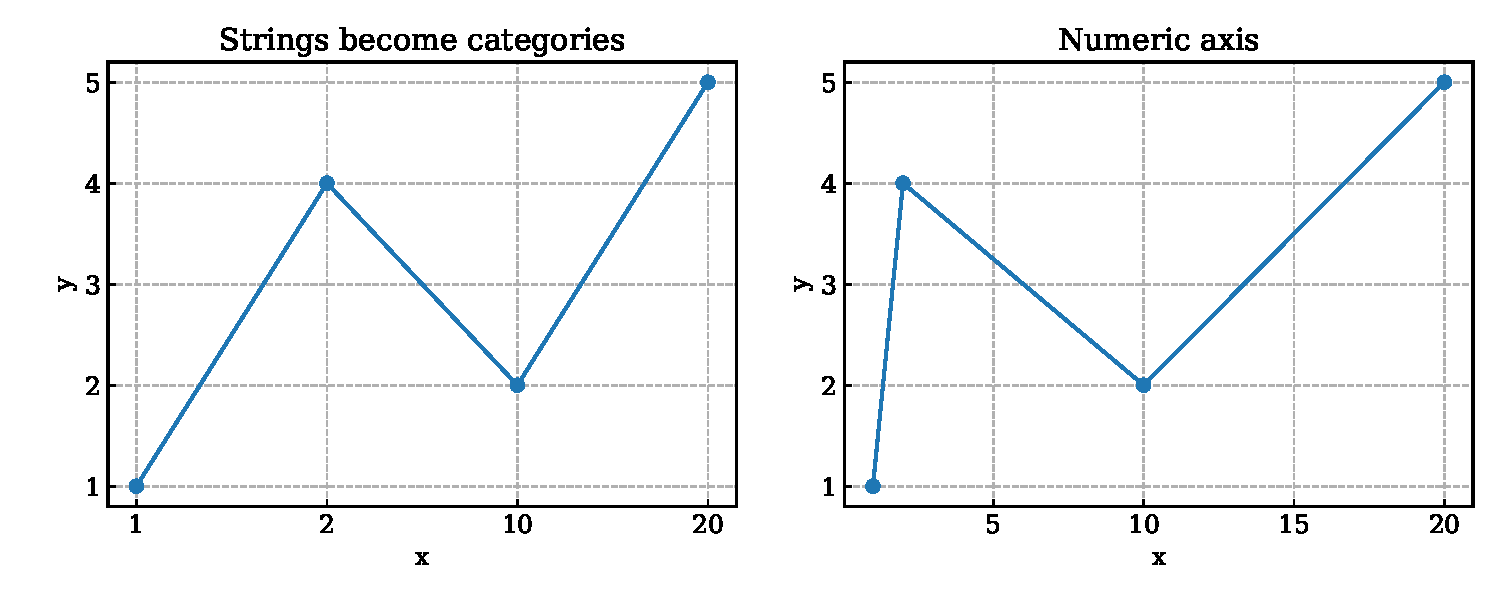
\includegraphics[width=0.92\linewidth]{string_axis_example.pdf}
\caption{文字列軸と数値軸の違い。左は \code{"1"}, \code{"2"}, \code{"10"}, \code{"20"} をカテゴリとして並べており、右は数値として扱っている。}
\label{fig:string-axis-example}
\end{figure}

\subsection{\code{savefig} と余白調整の順序}

長いラベルや図外の凡例は、保存領域からはみ出す場合がある。\code{tight\_layout()}、\code{constrained\_layout=True}、または \code{bbox\_inches="tight"} の効果を保存したファイルで確認する。再現可能なスクリプトでは、描画、余白調整、保存の順序を固定する。対数軸へ渡す値は正でなければならない。

\subsection{公式資料における作図例の検索}

ここまでの各節では、基本的な描画、レイアウト、オブジェクトの役割、保存方法を説明した。実際の作図では、目的に近い例を公式資料から探すと、利用できる図種や引数を把握しやすい。特に次の 4 つは参照頻度が高い。

\begin{itemize}
\item Quick start~\cite{matplotlib_quick_start}
\item Plot types~\cite{matplotlib_plot_types}
\item Gallery~\cite{matplotlib_gallery}
\item Cheatsheets~\cite{matplotlib_cheatsheets}
\end{itemize}

\code{Plot types} は図種ごとの選択肢、\code{Gallery} は完成例と実装、\code{Cheatsheets} は主要な引数と書式、\code{Quick start} は \code{Figure} と \code{Axes} の基本構造を示す。目的に近い公式例を選び、入力データ、軸、単位、保存形式を解析条件に合わせて変更する。

\section{章末課題：地震カタログと発生間隔の可視化}

USGS データと第~\ref{chap:numpy}~章で作成した \(\Delta t\) 配列がない場合は、次の小規模データを共通入力に用いよ。課題では画面表示だけで終わらせず、指定したファイルを保存し、保存後に \code{Path(...).exists()} で存在を確認せよ。

\begin{lstlisting}[language=Python]
import numpy as np

longitude = np.array([140.0, 141.2, 139.5, 142.0, 138.7])
latitude = np.array([35.0, 36.1, 34.8, 37.0, 33.9])
magnitude = np.array([3.2, 4.1, 2.8, 4.8, 3.7])
dt = np.array([1.0, 4.0, 12.0, 60.0, 180.0, 900.0, 3600.0])
\end{lstlisting}

\begin{enumerate}
\item \textbf{全球地震分布の散布図}。
USGS の CSV から \code{longitude}、\code{latitude}、\code{mag} を読み、横軸を経度、縦軸を緯度とする散布図を作れ。点の色でマグニチュードを表し、軸ラベル、カラーバー、タイトルを付けたうえで \code{figures/usgs\_global\_scatter.pdf} へ保存せよ。
\code{fig, ax = plt.subplots()} の返り値、\code{scatter = ax.scatter(...)} の返り値、\code{fig.colorbar(scatter, ax=ax)} の第 1 引数と \code{ax} 引数の役割を説明せよ。\code{scatter.get\_array()} がマグニチュード配列と一致し、\code{len(fig.axes)} がカラーバーを含めて 2 になることを確認せよ。

\item \textbf{発生間隔ヒストグラムの対数表示}。
第~\ref{chap:numpy}~章で作った \(\Delta t\) 配列を用い、発生間隔ヒストグラムを描け。縦軸を対数表示とし、横軸を線形尺度とした場合と対数尺度とした場合について、短い発生間隔の分解能、長時間側の裾の範囲、空のビンの数を比較せよ。図中にはビンの意味が分かる軸ラベルと単位を明記せよ。
線形ビンの図と \code{np.logspace()} で作った対数ビンの図を 2 枚の Axes に並べ、\code{figures/interval\_comparison.pdf} へ保存せよ。\code{ax.set\_yscale("log")} と \code{ax.set\_xscale("log")} がデータ値そのものを変換するのではなく、Axis の表示尺度を変えることを説明せよ。0 以下の値を対数軸へ置けない理由も述べよ。

\item \textbf{発展課題}。
通常の散布図では、点がどの海溝や列島に沿って並んでいるかは読み取りにくい。海岸線付きの地図へ重ねたい場合は、Matplotlib だけではなく地図投影を扱う \code{cartopy} が必要になる。\code{cartopy} を導入し、同じ地震データを海岸線付きの地図へ重ねよ。必要な出発点は、
\begin{itemize}
\item \code{projection=ccrs.PlateCarree()} による地図 Axes の作成
\item \code{scatter} 側への \code{transform=ccrs.PlateCarree()} の指定
\item \code{ax.coastlines()} による海岸線の描画
\item 全球図における \code{ax.set\_global()} の使用
\item 日本近海図における \code{ax.set\_extent([122, 154, 20, 50], crs=ccrs.PlateCarree())} の使用
\end{itemize}
である。これらの使い方を検索し、地図付きの散布図を作成せよ。
最小コードは、\code{import cartopy.crs as ccrs}、\code{fig, ax = plt.subplots(subplot\_kw=\{"projection": ccrs.PlateCarree()\})}、\code{ax.set\_global()}、\code{ax.coastlines()}、\code{ax.scatter(longitude, latitude, c=magnitude, transform=ccrs.PlateCarree())} の順に組み立てられる。\code{projection} は地図を描く Axes の座標系、\code{transform} は入力データの座標系を指定する。\code{figures/usgs\_map.pdf} を保存し、両者を同じ値にしていても役割が異なることを説明せよ。Cartopy が未導入なら、実行した導入コマンドと、導入前に出た例外名を記録せよ。
\end{enumerate}

可視化によって分布の形、外れ値、残差の傾向を確認できると、次に検討すべき数値計算を選びやすくなる。次章では、図から得た仮説を定量化するために、SciPy の統計分布、フィット、補間、信号処理を扱う。

\chapter{SciPy による数値計算とフィット}
\label{chap:scipy}

SciPy\index{scipy@SciPy|textbf} は、NumPy 配列を入力として統計、補間、信号処理、最適化、数値積分を行うライブラリ群である。本章では、分布モデル、パラメータ推定、曲線フィット、補間、信号処理と、それぞれの適用条件を扱う。

\section{分布モデルとパラメータ推定}

\subsection{NumPy 配列を入力とする専門計算機能}

SciPy の多くの関数は NumPy 配列を入力とし、NumPy 配列またはスカラーを返す。したがって、入力の \code{shape} と \code{dtype}、返り値の意味を NumPy の配列操作と対応付ける。目的と subpackage の対応は次のとおりである。

\begin{itemize}
\item \code{scipy.stats}\index{scipy@SciPy!stats@\code{scipy.stats}|textbf}: 分布、検定、要約統計
\item \code{scipy.optimize}: 最適化、非線形最小二乗、\code{curve\_fit}\index{scipy@SciPy!curve\_fit@\code{curve\_fit}|textbf}
\item \code{scipy.interpolate}\index{scipy@SciPy!interpolate@\code{scipy.interpolate}|textbf}: 補間
\item \code{scipy.signal}\index{scipy@SciPy!signal@\code{scipy.signal}|textbf}: フィルタ、ピーク検出、相関、スペクトル処理
\item \code{scipy.integrate}\index{scipy@SciPy!integrate@\code{scipy.integrate}|textbf}: 数値積分
\item \code{scipy.constants}\index{scipy@SciPy!constants@\code{scipy.constants}|textbf}: 物理定数
\end{itemize}

要素ごとの演算や基本的な集計には NumPy を用い、確率分布、最適化、補間、信号処理などの専用アルゴリズムが必要な場合に、対応する SciPy の subpackage を選ぶ。

\subsection{関数形の仮定とパラメータ推定}

分布の幅、減衰曲線の時定数、波形のピーク時刻を推定するには、それぞれモデル推定、非線形最小二乗、ピーク検出の条件を定める必要がある。SciPy は、これらの計算と推定結果の評価に用いる関数を提供する。

フィットでは、仮定した関数形のパラメータをデータから推定する。関数形の選択には物理的または統計的な根拠が必要であり、推定値の解釈にはフィット範囲、ビン幅、外れ値処理、残差、不確かさの確認が必要となる。

フィットの目的は、仮定したモデルのパラメータをデータから推定することである。分布の中心、幅、時定数などを比較可能な量として得るには、推定値だけでなく、不確かさ、フィット範囲、残差、モデルの適用条件も確認する。

\subsection{正規分布と指数分布}

多数の独立な微小変動の和は、条件を満たせば正規分布で近似できる。一定の発生率を持つ Poisson 過程では、事象間の待ち時間が指数分布に従う。対象データがこれらの仮定を満たすかは、生成過程、残差、代替モデルとの比較によって検証する。

たとえば、平均 \(\mu\)、標準偏差 \(\sigma\) のガウシアンは
\[
p(x) = \frac{1}{\sqrt{2\pi}\sigma}
\exp\!\left[-\frac{(x-\mu)^2}{2\sigma^2}\right]
\]
で書ける。また、時定数 \(\tau\) の指数分布は
\[
p(t) = \frac{1}{\tau} \exp\!\left(-\frac{t}{\tau}\right)
\qquad (t \ge 0)
\]
である。SciPy の分布オブジェクトは、確率密度、累積分布、分位点、乱数生成を共通のインタフェースで提供する。

\section{統計・フィット・補間・信号処理}

\subsection{\code{scipy.stats} による要約統計と分布}

配列の要素数、中心、広がり、形状を数値で確認する方法を示す。

\begin{lstlisting}[language=Python]
import numpy as np
from scipy import stats

values = np.array([1.2, 0.9, 1.5, 1.1, 0.8])

summary = stats.describe(values)
print(summary.nobs)
print(f"{summary.mean:.3f}")
print(f"{summary.variance:.3f}")
\end{lstlisting}

この例では、要素数、平均、分散が順に表示される。

\begin{lstlisting}[numbers=none, xleftmargin=2\zw]
5
1.100
0.075
\end{lstlisting}

\code{stats.describe()} は、要素数、平均、分散、最小値、最大値、歪度、尖度を名前付きタプルとして返す。分散の既定は \code{ddof=1} であり、NumPy の \code{var()} の既定とは異なる。各統計量の定義と単位を確認してから利用する。

SciPy の分布オブジェクトは、確率密度関数や累積分布関数を同じ API で扱える。

\begin{lstlisting}[language=Python]
x = np.linspace(-3.0, 3.0, 7)
pdf = stats.norm.pdf(x, loc=0.0, scale=1.0)
cdf = stats.norm.cdf(x, loc=0.0, scale=1.0)

print(pdf)
print(cdf)
\end{lstlisting}

\code{pdf} と \code{cdf} を同じ点列で評価すると、次のような値が得られる。

\begin{lstlisting}[numbers=none, xleftmargin=2\zw]
[0.00443185 0.05399097 0.24197072 0.39894228 0.24197072 0.05399097
 0.00443185]
[0.0013499  0.02275013 0.15865525 0.5        0.84134475 0.97724987
 0.9986501 ]
\end{lstlisting}

\code{pdf} は確率密度関数、\code{cdf} は累積分布関数、\code{rvs} は乱数生成、\code{ppf} は累積確率から分位点を求める逆関数に対応する。正規分布では \code{loc} は平均、\code{scale} は標準偏差であるが、これらの引数の意味は分布ごとに確認する。

ここで \code{pdf} は確率密度 \(p(x)\)、\code{cdf} はその積分
\[
F(x) = \int_{-\infty}^{x} p(t)\,dt
\]
に対応する。したがって、\code{stats.norm.cdf(x)} は「\(x\) 以下に入る確率」を返している。

\subsection{\code{curve\_fit} によるパラメータ推定}

\code{scipy.optimize.curve\_fit} は、利用者が定義したモデル関数のパラメータを非線形最小二乗法で推定する。\code{scipy.stats} が実装済みの確率分布に対する密度評価やパラメータ推定を提供するのに対し、\code{curve\_fit} には任意のモデル関数を渡せる。

\begin{lstlisting}[language=Python]
from scipy.optimize import curve_fit

def linear_model(x, a, b):
    return a * x + b

xdata = np.array([0.0, 1.0, 2.0, 3.0, 4.0])
ydata = np.array([1.1, 2.0, 3.2, 4.1, 5.1])

linear_params, linear_cov = curve_fit(linear_model, xdata, ydata)
linear_errors = np.sqrt(np.diag(linear_cov))

print(linear_params)
print(linear_errors)
\end{lstlisting}

この線形フィットでは、傾きと切片、および共分散行列から求めた標準誤差が次のように得られる。

\begin{lstlisting}[numbers=none, xleftmargin=2\zw]
[1.01 1.08]
[0.02516611 0.06164414]
\end{lstlisting}

\code{linear\_params} は推定パラメータ、\code{linear\_cov} は共分散行列である。対角成分の平方根が各パラメータの標準誤差に対応する。上の例では \code{linear\_params[0]} が傾き、\code{linear\_params[1]} が切片である。非対角成分はパラメータ間の共分散を表すため、相関を調べる場合は各パラメータの標準偏差で規格化する。\code{curve\_fit()} の出力は、仮定したモデル、残差の定義、\code{sigma} の指定に依存する。

上の直線モデル \(f(x; a, b) = ax + b\) なら、\code{curve\_fit()} は概ね
\[
S(a, b) = \sum_i \left[y_i - (a x_i + b)\right]^2
\]
を小さくする \(a\) と \(b\) を探していると考えればよい。より一般には、モデル \(f(x; \mathbf{p})\) に対して
\[
S(\mathbf{p}) = \sum_i \left[y_i - f(x_i; \mathbf{p})\right]^2
\]
という残差二乗和を最小化している。

得られた推定値は、データとモデルを重ねた図、別条件のデータ、単位、残差と照合する。SciPy の各関数についても、入力、返り値、仮定、失敗条件を確認する。

\section{モデル選択・重み付け・残差評価}

モデル推定では、次の項目を順に記録する。

\begin{enumerate}
\item 作図に基づく候補関数の検討
\item フィット範囲の決定
\item 必要に応じた妥当な初期値の設定
\item データとフィット曲線の重ね描き
\item 推定値と残差の確認
\end{enumerate}

モデルの定義とデータの確認を省いて \code{curve\_fit()} を実行しても、推定値の妥当性を判断できない。フィットは、モデルという仮説をデータと残差によって検証する手続きである。

\subsection{初期値、制約、残差}

モデルによっては、初期値や制約を与えないと不安定になる。

\begin{lstlisting}[language=Python]
def exp_model(x, a, tau, c):
    return a * np.exp(-x / tau) + c

x_decay = np.linspace(0.0, 8.0, 40)
rng = np.random.default_rng(31)
y_decay = 4.0 * np.exp(-x_decay / 2.5) + 0.3
y_decay += rng.normal(loc=0.0, scale=0.05, size=x_decay.size)

exp_params, exp_cov = curve_fit(
    exp_model,
    x_decay,
    y_decay,
    p0=[5.0, 2.0, 0.0],
    bounds=([0.0, 0.0, -np.inf], [np.inf, np.inf, np.inf]),
)
\end{lstlisting}

\code{p0}\index{p0@\code{p0}|textbf} は初期値、\code{bounds}\index{bounds@\code{bounds}|textbf} はパラメータ範囲である。どちらも収束を保証するものではないが、物理的にあり得ない範囲を除外する際に有効である。モデルによっては、初期値によって収束先が変わる。また、物理的に非負であるパラメータには、0 を下限とする制約を指定できる。

フィット結果の図には、関数形、推定パラメータ、データ系列を識別できる情報を記載する。凡例を用いる場合は、データや曲線を隠さない位置を選び、複数の図で同じ書式を用いる。

\begin{lstlisting}[language=Python]
import numpy as np
import matplotlib.pyplot as plt
from scipy import stats

rng = np.random.default_rng(37)
values = rng.normal(loc=3.0, scale=0.8, size=3000)
mean, sigma = stats.norm.fit(values)
x = np.linspace(values.min(), values.max(), 300)

fig, ax = plt.subplots()
ax.hist(values, bins=40, density=True, alpha=0.7, label="sample")
ax.plot(
    x,
    stats.norm.pdf(x, loc=mean, scale=sigma),
    linewidth=2.0,
    label=(
        "fit: "
        r"$f(x)=\frac{1}{\sqrt{2\pi}\sigma}"
        r"\exp\!\left[-\frac{(x-\mu)^2}{2\sigma^2}\right]$"
        "\n"
        + fr"$\mu={mean:.2f},\ \sigma={sigma:.2f}$"
    ),
)
ax.legend(loc="upper right")
\end{lstlisting}

図~\ref{fig:distribution-examples} では、フィットした分布名と推定パラメータを凡例へ記載している。左パネルは上の正規乱数と同じ入力を用い、右パネルは同じ乱数生成器で続けて生成した時定数 2.5 s、3000 個の指数乱数を用いる。本文には推定方法と解釈、キャプションには図の対象と条件、凡例には系列の識別情報を置く。

\begin{lstlisting}[language=Python]
model_y = linear_model(xdata, *linear_params)
residual = ydata - model_y
print(residual)
\end{lstlisting}

最適化が終了して推定値を返したことは、モデルの妥当性を保証しない。残差を横軸に対して表示し、符号や大きさに系統的な構造が残っていないか、特定の範囲だけ偏差が大きくないかを確認する。

外れ値やモデルの適用範囲外にある領域を含めると、推定値が変化する場合がある。フィット範囲と除外条件を推定値とともに記録する。

\begin{lstlisting}[language=Python]
mask = (xdata >= 0.0) & (xdata <= 3.0)
range_params, range_cov = curve_fit(
    linear_model,
    xdata[mask],
    ydata[mask],
)
\end{lstlisting}

フィット範囲は、モデルを適用する領域を定義する解析条件である。範囲をデータ確認後に変更した場合は、その判断基準と変更前後の結果も報告する。

\subsection{\code{sigma} を使った重み付きフィット}

物理の実データでは、各データ点の不確かさが等しいとは限らない。点ごとの標準偏差が既知であり、その大きさが異なる場合は、\code{sigma}\index{sigma@\code{sigma}|textbf} を使って残差を標準偏差で規格化する。\code{sigma} を与えないフィットはすべての点を等しい重みで扱うため、不確かさが点ごとに異なるデータでは目的と一致しない場合がある。

\begin{lstlisting}[language=Python]
y_err = np.array([0.2, 0.2, 1.5, 0.2, 0.2])

weighted_params, weighted_cov = curve_fit(
    linear_model,
    xdata,
    ydata,
    sigma=y_err,
    absolute_sigma=True,
)
\end{lstlisting}

この定義では、\code{sigma} が大きい点ほど規格化残差が小さくなり、目的関数への寄与が小さくなる。図~\ref{fig:fit-sigma} は、その差を模式的に示している。

\begin{figure}[htbp]
\centering
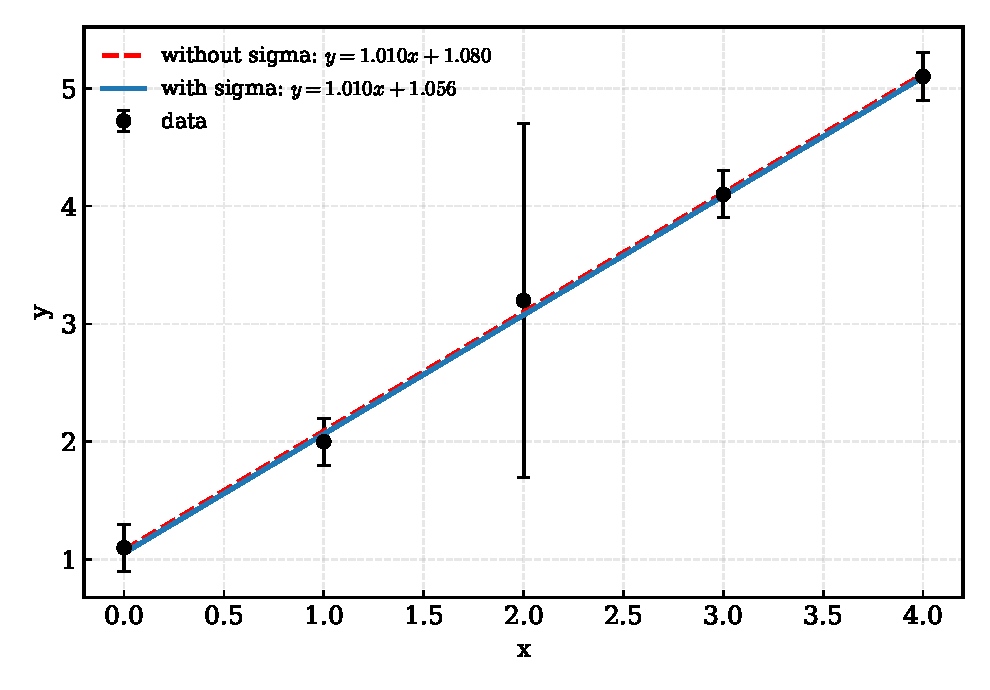
\includegraphics[width=0.7\linewidth]{fit_sigma_comparison.pdf}
\caption{\code{sigma} の有無によるフィット結果の違い。不確かさが点ごとに異なる場合、\code{sigma} の指定によって各残差の寄与が変わる。}
\label{fig:fit-sigma}
\end{figure}

\code{sigma} には、通常 \code{ydata} の各点に対応する 1 次元配列を渡す。このとき最小化される量は
\[
\chi^2(\mathbf{p}) = \sum_i
\left(
\frac{y_i - f(x_i; \mathbf{p})}{\sigma_i}
\right)^2
\]
と書けるので、\(\sigma_i\) が大きい点ほど目的関数への寄与は小さく、\(\sigma_i\) が小さい点ほど大きくなる。独立な Poisson 計数で平均値を観測数 \(N\) によって推定し、正規近似が妥当な範囲では、標準偏差を \(\sqrt{N}\) で近似する場合がある。低計数や重み付き計数には、その近似を機械的に適用しない。

\code{absolute\_sigma=True} は、共分散の計算に \code{sigma} の絶対的な大きさを使う指定である。渡した値が適切な標準偏差かどうかを、この設定が検証するわけではない。これを \code{False} のままにすると、\code{sigma} は相対的な重みとしては使われるが、共分散行列の大きさは残差のばらつきに合わせてあとから再スケーリングされる。そのため、推定値の重み付けだけでなく誤差評価まで行いたいなら、\code{sigma} の意味を明確にした上で \code{absolute\_sigma} の設定も意識する必要がある。

図~\ref{fig:fit-sigma} は、点ごとの不確かさを重みに反映した場合と、全点を等しい重みで扱った場合の違いを示している。どちらを採用するかは、\code{sigma} が測定の標準偏差を表すか、各点を同じ重みで比較する解析なのかによって決まる。

\code{curve\_fit()} の共分散とその対角成分から求める標準誤差は、解の近傍での線形近似に依存する~\cite{scipy_curvefit}。強い非線形性やパラメータ間の縮退がある場合には信頼できないことがある。1 次元の \code{sigma} による上の式は各点の誤差を独立とする。相関を扱うには共分散行列を渡す方法があり、通常の呼び出しは横軸 \code{xdata} の測定誤差を考慮しない。

\subsection{\code{scipy.interpolate} による補間}

補間は、測定点の間における値を仮定した関数形から推定する操作である。ここでは、1 次元データに対する区分線形補間を扱う。

\begin{lstlisting}[language=Python]
from scipy.interpolate import make_interp_spline

x = np.array([0.0, 1.0, 2.0, 4.0])
y = np.array([0.0, 2.0, 1.0, 3.0])

linear_interp = make_interp_spline(x, y, k=1)
x_new = np.array([0.5, 1.5, 3.0])
y_new = linear_interp(x_new, extrapolate=False)

print(y_new)
\end{lstlisting}

補間点 \code{x\_new} に対しては、次の値が返る。

\begin{lstlisting}[numbers=none, xleftmargin=2\zw]
[1.  1.5 2. ]
\end{lstlisting}

入力の \code{x} は重複がなく、昇順に並んでいる必要がある。区分線形補間は測定点を通る連続関数だが、接続点で傾きが不連続になり得る。上の \code{extrapolate=False} は入力範囲の外で \code{NaN} を返し、外挿を行わない指定である。範囲外まで同じ傾向が続くとは限らない。

線形補間では、各区間 \(x_i \le x \le x_{i+1}\) で
\[
y(x) = y_i + \frac{y_{i+1}-y_i}{x_{i+1}-x_i}(x-x_i)
\]
という一次式を使っている。したがって、測定点の間では直線でつながるが、測定範囲の外ではこの式をそのまま信じる根拠はない。

\subsection{\code{scipy.signal} による平滑化とピーク検出}

波形や時系列では、ピークの検出や軽い平滑化がよく必要になる。

\begin{lstlisting}[language=Python]
from scipy.signal import savgol_filter, find_peaks

x = np.linspace(0.0, 20.0, 200)
signal = np.sin(x) + 0.15 * np.random.default_rng(7).normal(size=x.size)

smooth = savgol_filter(signal, window_length=11, polyorder=3)
peaks, props = find_peaks(smooth, height=0.7, distance=15)

print(peaks)
print(np.round(props["peak_heights"], 3))
\end{lstlisting}

この例では、検出されたピーク位置とその高さが次のように表示される。

\begin{lstlisting}[numbers=none, xleftmargin=2\zw]
[ 13  76 138]
[0.977 1.048 0.994]
\end{lstlisting}

\code{savgol\_filter()} は局所多項式によって平滑化する。\code{find\_peaks()} は高さ、試料点間の距離、prominence などの条件でピーク候補を抽出する。検出条件をサンプリング間隔と対応付け、既知の合成波形で検出率と誤検出を確認してから実データへ適用する。

\subsection{\code{scipy.integrate} と \code{scipy.constants}}

\code{scipy.integrate} は離散点または関数の数値積分を、\code{scipy.constants} は物理定数の数値と単位情報を提供する。

\begin{lstlisting}[language=Python]
from scipy import constants
from scipy.integrate import simpson

x = np.linspace(0.0, np.pi, 101)
y = np.sin(x)

area = simpson(y, x=x)
print(area)
print(constants.c)
\end{lstlisting}

この積分値と光速定数は、次のように出力される。

\begin{lstlisting}[numbers=none, xleftmargin=2\zw]
2.0000000108245044
299792458.0
\end{lstlisting}

\code{simpson()} は、ここでは
\[
\int_0^\pi \sin x\,dx = 2
\]
という積分を、離散点 \((x_i, y_i)\) から数値的に評価している。したがって、\code{simpson(y, x=x)} は「\(y(x)\) をサンプル点から積分する関数」と読めばよい。また、\code{constants.c} は
\[
c = 299792458\ \mathrm{m\,s^{-1}}
\]
を表す定数である。\code{constants.c} 自体は単位を保持しない浮動小数点数なので、単位を演算中も保持する必要がある場合は、次章の Astropy の \code{Quantity} と定数オブジェクトを用いる。

\section{モデル・制約・外挿に関する注意点}

\subsection{モデル選択の理由がないままフィットしない}

ガウシアン、指数、直線の選択には、物理的または統計的な仮定が必要である。曲線がデータ点の近くを通ることだけでは、モデルの生成過程やパラメータの解釈を正当化できない。

\subsection{初期値と制約を無視しない}

非線形フィットは、初期値次第で別の極小へ落ちたり、収束しなかったりする。\code{curve\_fit()} が値を返したからといって、それが唯一の解だとは限らない。複数の初期値で試す、図へ重ねて見る、残差を見る、といった確認が必要である。

\subsection{補間と外挿を混同しない}

\code{make\_interp\_spline()} などの補間関数は、観測点の間を埋めるための道具である。測定範囲の外まで同じ関係が続く根拠は補間からは得られない。外側を予測する場合は、外挿に用いるモデルと適用範囲を別に検討する。

\subsection{信号処理におけるサンプリング間隔}

\code{find\_peaks()} の \code{distance} やフィルタ長は、サンプル数で指定することが多い。したがって、時間軸が 1 サンプル 1 ns なのか 10 ns なのかで、同じ数値でも意味が変わる。コード中の数字をそのまま流用せず、軸の単位へ戻して考える必要がある。

\section{発生間隔分布のモデル比較}

SciPy は、解析の中で次のような役割を持つ。

\begin{enumerate}
\item \code{stats} による分布形状と要約統計の確認
\item \code{signal} によるピーク候補の抽出と平滑化
\item \code{interpolate} による校正曲線・補助曲線の作成
\item \code{optimize} によるモデルパラメータの推定
\item \code{integrate} と \code{constants} による計算の完結
\end{enumerate}

SciPy は、入力配列の物理的意味や、採用すべきモデルを自動では決めない。特にフィットでは、データ範囲、重み、残差、推定値の不確かさを確認し、採用した条件を結果とともに記録する必要がある。

ここまで見てきた SciPy は、主に「数値をどう計算するか」を受け持つ道具である。時刻系、単位、座標系、FITS のように「数値そのものの意味付け」まで含めて扱いたくなったところで、次章の Astropy が必要になる。SciPy は計算アルゴリズム、Astropy は物理量や観測量の表現を担当すると考えると、章のつながりも見えやすい。

本文を読み終えた後で関数名や引数を確認したいときは、SciPy User Guide~\cite{scipy_user_guide} を起点にすると探しやすい。分布や検定は Statistics~\cite{scipy_stats}、フィットや最適化は Optimization~\cite{scipy_optimize}、補間は Interpolation~\cite{scipy_interpolate}、波形処理は Signal processing~\cite{scipy_signal}、数値積分は Integration~\cite{scipy_integrate} が対応している。本章は、それらを解析で使う順に並べ替えて説明した。

\section{章末課題：分布モデルとフィットの演習}

この章の課題は、既知の分布による API と結果の読み方の検証、および実データに対するモデルの検討という二段階からなる。次のコードが検証用データを生成する。乱数シードを固定しているため、同じライブラリ環境では同じ入力を再現できる。

\begin{lstlisting}[language=Python]
import numpy as np

rng = np.random.default_rng(20260412)
synthetic_dt = rng.exponential(scale=120.0, size=5000)
x = np.linspace(0.0, 10.0, 80)
y_true = 2.5 * x + 1.2
sigma = np.full_like(x, 0.5)
y_obs = y_true + rng.normal(scale=sigma)
\end{lstlisting}

実データに当てる分布と関数を、最初から決め打ちしてはならない。まず図を描いて特徴を観察し、比較する量と近似を試す範囲を判断せよ。ヒストグラムと累積分布の選択、短時間側の取扱い、対数軸の採否についても、その理由とともに記録せよ。

\begin{enumerate}
\item \textbf{既知の指数分布による推定方法の検証}。
\code{scipy.stats.expon.fit(synthetic\_dt, floc=0)} で指数分布のパラメータを推定せよ。\code{floc=0} は位置母数を 0 に固定する指定であり、返り値は \code{loc} と \code{scale} の順である。推定された \code{scale} が生成時の 120 秒に近いことを確認し、標本平均とも比較せよ。許容範囲を 115 秒から 125 秒として自動確認する \code{assert} も記述せよ。

\item \textbf{重み付き直線フィットと残差の確認}。
\code{curve\_fit()} を使い、\code{y\_obs} を \(y=ax+b\) へフィットせよ。\code{sigma=sigma}、\code{absolute\_sigma=True} を指定し、推定値 \code{popt} と共分散行列 \code{pcov} を受け取る。傾きが 2.3 から 2.7、切片が 0.7 から 1.7 の範囲に入ることを確認せよ。\code{np.sqrt(np.diag(pcov))} が各パラメータの標準不確かさを与えること、\code{y\_obs - model(x, *popt)} が残差になることを説明し、データ、フィット線、残差を 2 段の図へ保存せよ。

\item \textbf{実データの発生間隔分布と fit 方針の決定}。
第~\ref{chap:numpy}~章で作った \(\Delta t\) 配列がある場合は、等間隔ビンのヒストグラム、対数ビンのヒストグラム、経験累積分布のうち少なくとも 2 通りを作成せよ。その上で、指数分布を含む候補を比較し、採用するモデルとフィット範囲を決定せよ。1 問目の検証用データと異なり、実データが単一の指数分布に従う保証はない。モデルを採用した根拠、除外した範囲、残差または適合度を記録せよ。

\item \textbf{解析上の選択に対する感度評価}。
3 問目と少なくとも 1 条件を変えて推定を繰り返せ。ビン幅、フィット範囲、短時間側の扱い、重み、関数形などから選び、推定値と不確かさがどの程度変化したかを表にまとめよ。結果が変わったという事実だけでなく、どのデータ点の寄与が変化したためかを図と残差から説明せよ。

実データでは、検索期間・地域、使用したイベント種別、マグニチュードの型を記録する。USGS の CSV には \code{magType} などの列があり~\cite{usgs_csv}、異なる尺度や検出能力の地域を混ぜると単一のモデルで説明できない場合がある。

\item \textbf{発展課題：マグニチュード分布と Gutenberg--Richter 関係}。
USGS カタログのマグニチュード \(M\) について、度数分布と累積件数 \(N(\geq M)\) を作り、カタログが十分に完全とみなせる下限 \(M_c\) を検討せよ。\(M\geq M_c\) の範囲で Gutenberg--Richter 関係~\cite{gutenberg_richter_1944}
\[
\log_{10}N(\geq M)=a-bM
\]
が成り立つかを調べる。この関係は、地震規模に対するべき乗則を、対数尺度であるマグニチュード \(M\) で表したものである。

累積件数の点は同じイベントを共有するため、独立な Poisson 変数として \(\chi^2\) を解釈できない。推定には、重ならないマグニチュード区間の度数に対する計数モデル、または個々の \(M\) に対する尤度法を用いよ。累積分布は表示だけに用い、推定量と区別せよ。日本近海または全球を対象とし、期間、空間範囲、\(M_c\)、ビン、イベント数、推定法、不確かさ、残差を明示せよ。
\end{enumerate}

SciPy は数値配列に対する計算を担うが、物理単位、時刻系、天球座標の意味までは自動的に補わない。次章では、Astropy によって数値へ単位や座標系を保持し、SciPy や表処理ライブラリとの間で受け渡す方法を扱う。

\chapter{Astropy による時刻・単位・\mbox{天体データ処理}}
\label{chap:astropy}

Astropy\index{astropy@Astropy|textbf} は、単位付き物理量、時刻系、天球座標系、FITS、天文向け表を扱うライブラリである。単位、時刻系、座標系を数値とは別の文字列として管理すると、演算時に対応関係を失う可能性がある。本章では、これらの情報を数値と同じオブジェクトに保持し、変換、演算、表および FITS への保存を行う方法を扱う。

\section{数値と単位・時刻・座標の一元的な管理}

\subsection{数値への単位・時刻・座標情報の付与}

Astropy の中心的な発想は、「数値そのもの」ではなく「何の単位で、どの時刻系で、どの座標系なのか」までオブジェクトへ持たせることである。例えば 100 という値だけでは、100 ns なのか 100 ms なのか分からない。Astropy の \code{Quantity}\index{quantity@\code{Quantity}|textbf} を使えば、この曖昧さを減らせる。

\begin{lstlisting}[language=Python]
import astropy.units as u

time_window = 250 * u.ns
speed = 299792458 * u.m / u.s
distance = speed * time_window

print(distance)
print(distance.to(u.m))
\end{lstlisting}

この計算では、単位付きのまま距離が評価され、次のように表示される。

\begin{lstlisting}[numbers=none, xleftmargin=2\zw]
74.9481145 m
74.9481145 m
\end{lstlisting}

この例では、\code{250 * u.ns} という時点で「250 ns」という意味が値に埋め込まれている。式の途中で単位を落とさない限り、単位換算はライブラリが引き受ける。

数式で書けば、ここで行っているのは
\[
d = v \Delta t
\]
である。特に \(v = c\) とみなすなら、250 ns の時間窓に対応する距離 \(d = c \Delta t\) をそのまま安全に計算できる。

\subsection{時刻系・座標系を属性として保持する理由}

観測データでは、UTC、TAI、TT、MJD、JD、Unix time が混在することがある。文字列の分解だけで相互変換すると、時刻系のオフセットとうるう秒が計算に反映されず、時刻差を誤る可能性がある。Astropy の \code{Time} は、時刻形式と時刻系を属性として保持する。

\section{単位・時刻・座標・表・FITS の操作}

\subsection{\code{units} と \code{Quantity}}

単位付き計算の基本は \code{Quantity} である。

\begin{lstlisting}[language=Python]
import astropy.units as u

length = 3.2 * u.m
time = 12.5 * u.ns
velocity = length / time

print(velocity)
print(velocity.to(u.m / u.s))
\end{lstlisting}

単位変換の結果は次の通りである。

\begin{lstlisting}[numbers=none, xleftmargin=2\zw]
0.256 m / ns
256000000.0 m / s
\end{lstlisting}

\code{to()} は、指定した単位へ換算した \code{Quantity} を返す。\code{.value} は単位情報を除いた数値を返すため、単位を受け取らない関数へ渡す直前など、数値だけが必要な箇所に使用を限定する。

この計算は
\[
v = \frac{L}{t}
\]
に対応しており、具体的には
\[
v = \frac{3.2\ \mathrm{m}}{12.5\ \mathrm{ns}}
= 0.256\ \mathrm{m/ns}
= 2.56 \times 10^8\ \mathrm{m/s}
\]
である。コードの出力をこの換算式と照合すれば、桁と SI 接頭語の対応を検証できる。

\subsection{物理定数}

Astropy には物理定数も入っている。SciPy の \code{constants} と似ているが、こちらは単位付きで返る点が大きい。

\begin{lstlisting}[language=Python]
from astropy.constants import c, k_B

print(c)
print(k_B)
\end{lstlisting}

Astropy の定数オブジェクトを表示すると、値だけでなく単位と参照元も確認できる。

\begin{lstlisting}[numbers=none, xleftmargin=2\zw]
  Name   = Speed of light in vacuum
  Value  = 299792458.0
  Uncertainty  = 0.0
  Unit  = m / s
  Reference = CODATA 2022
  Name   = Boltzmann constant
  Value  = 1.380649e-23
  Uncertainty  = 0.0
  Unit  = J / K
  Reference = CODATA 2022
\end{lstlisting}

この表示から、定数の値、単位、不確かさ、参照する定数体系を確認できる。

\subsection{\code{Time} による時刻表現}

Astropy の \code{Time}\index{time@\code{Time}|textbf} は、複数のフォーマットと複数の時刻系をまたいで扱える。

\begin{lstlisting}[language=Python]
from astropy.time import Time

t = Time("2026-04-12 12:34:56.123456789", format="iso", scale="utc")

print(t.mjd)
print(t.unix)
print(t.tai.iso)
\end{lstlisting}

同じ時刻を複数の表現へ変換すると、次の値が得られる。

\begin{lstlisting}[numbers=none, xleftmargin=2\zw]
61142.52426068816
1775997296.1234567
2026-04-12 12:35:33.123
\end{lstlisting}

\code{format="iso"} は入力形式、\code{scale="utc"} は時刻系を表す。\code{mjd} と \code{unix} は同じ時刻の別形式を返し、\code{tai.iso} は時刻系を TAI へ変換して ISO 形式で返す。

たとえば、修正ユリウス日 MJD は
\[
\mathrm{MJD} = \mathrm{JD} - 2400000.5
\]
で定義される。Astropy の \code{Time} は、時刻形式と時刻系を属性として保持し、それらの変換を同じオブジェクト上で行う。

\subsection{時刻差と \code{TimeDelta}}

差分計算も \code{Time} のまま行える。\code{TimeDelta}\index{timedelta@\code{TimeDelta}|textbf} によって、差分の単位変換も一貫して扱える。

\begin{lstlisting}[language=Python]
from astropy.time import Time

t1 = Time("2026-04-12T12:00:00.000000100", format="isot", scale="utc")
t2 = Time("2026-04-12T12:00:00.000000320", format="isot", scale="utc")
dt = t2 - t1

print(f"{dt.to_value('s'):.9e}")
print(f"{dt.to_value('ns'):.3f}")
\end{lstlisting}

時刻差を秒と ns へ変換した結果は次の通りである。

\begin{lstlisting}[numbers=none, xleftmargin=2\zw]
2.200000182e-07
220.000
\end{lstlisting}

\code{TimeDelta} の既定の内部形式や表示は、入力形式と同じ単位とは限らない。そのため、出力では \code{to\_value("s")} や \code{to\_value("ns")} によって単位を明示する。秒境界や日付境界をまたぐ場合も、文字列を分解せずに差を計算できる。

ここで計算している時刻差は
\[
\Delta t = t_2 - t_1 = 220\ \mathrm{ns}
\]
である。\code{Time} どうしの減算は \code{TimeDelta} を返すため、時刻系に基づく差分と単位情報が結果に保持される。

\subsection{\code{SkyCoord} による座標変換}

Astropy の \code{coordinates} は、天球上の座標系を変換する。\code{SkyCoord}\index{skycoord@\code{SkyCoord}|textbf} はその中心となるクラスである。

\begin{lstlisting}[language=Python]
from astropy.coordinates import SkyCoord
import astropy.units as u

coord = SkyCoord(ra=150.0 * u.deg, dec=20.0 * u.deg, frame="icrs")
gal = coord.galactic

print(f"{gal.l.deg:.6f}")
print(f"{gal.b.deg:.6f}")
\end{lstlisting}

座標変換後の銀河経度と銀河緯度は次の通りである。

\begin{lstlisting}[numbers=none, xleftmargin=2\zw]
213.800977
50.263718
\end{lstlisting}

\code{ra} と \code{dec} には単位を付ける。これにより、入力角度が度またはラジアンのどちらで与えられたかが \code{SkyCoord} に保持される。

この操作は、赤道座標 \((\alpha, \delta)\) から銀河座標 \((l, b)\) への変換に対応する。天球上の回転そのものは自分で式を書かなくても、入力座標系と出力座標系を明示すれば Astropy が一貫して扱える。

\subsection{\code{Table} と \code{QTable}}

Astropy には表処理のために \code{Table}\index{table@\code{Table}|textbf} と \code{QTable}\index{qtable@\code{QTable}|textbf} がある。\code{QTable} は列へ単位を保持できる。

\begin{lstlisting}[language=Python]
from astropy.table import QTable
import astropy.units as u

table = QTable()
table["time"] = [0.0, 1.0, 2.0] * u.s
table["signal"] = [12.4, 10.1, 14.8] * u.mV
table["detector"] = ["A", "A", "B"]

print(table)
\end{lstlisting}

\code{QTable} を表示すると、列名だけでなく単位も一緒に確認できる。

\begin{lstlisting}[numbers=none, xleftmargin=2\zw]
time signal detector
 s    mV
---- ------ --------
0.0   12.4        A
1.0   10.1        A
2.0   14.8        B
\end{lstlisting}

\code{QTable} は \code{Quantity} 列を保持するため、単位付きの列をそのまま演算できる。一方、複雑な groupby、join、列演算を中心とする処理には pandas や Polars の機能を利用できる。単位とメタデータの保持、および必要な表操作の双方から中心となる表形式を選ぶ。

\subsection{Astropy Table と pandas の行き来}

Astropy の表と pandas の DataFrame は相互変換できるが、単位や時刻の情報が完全には残らないことがある。

\begin{lstlisting}[language=Python]
df = table.to_pandas()
print(df)
\end{lstlisting}

\code{to\_pandas()} で得た通常の pandas 列には、\code{Quantity} の単位属性はそのまま保持されない。変換前に列単位を記録し、変換後の数値へどの単位を対応させるかを明示する。マスク付き列と時刻列についても、欠損表現と型が変換前後で一致するかを確認する。

\subsection{\code{astropy.io.fits} による FITS の読み書き}

天文データでは FITS\index{fits@FITS|textbf} が標準的である。Astropy なら NumPy 配列やヘッダをそのまま扱える。

\begin{lstlisting}[language=Python]
import numpy as np
from astropy.io import fits

image = np.arange(9).reshape(3, 3)
hdu = fits.PrimaryHDU(image)
hdu.header["OBJECT"] = "test"
hdu.writeto("image.fits", overwrite=True)

with fits.open("image.fits") as hdul:
    data = hdul[0].data
    header = hdul[0].header

print(data.shape)
print(header["OBJECT"])
\end{lstlisting}

FITS を書いてから読み直すと、配列形状とヘッダ値は次のように確認できる。

\begin{lstlisting}[numbers=none, xleftmargin=2\zw]
(3, 3)
test
\end{lstlisting}

\code{fits.open()} は HDU のリストを返す。画像は \code{PrimaryHDU}、表は \code{BinTableHDU} などに格納される。\code{hdul.info()} で各 HDU の型、名前、次元を確認してから、対象のデータを読み込む。

\subsection{ASCII・ECSV 形式の読み込み}

Astropy の表入出力は FITS だけではない。\code{Table.read()} は ASCII、CSV、ECSV などにも対応している。

\begin{lstlisting}[language=Python]
from astropy.table import Table

tbl = Table.read("events.ecsv", format="ascii.ecsv")
print(tbl.colnames)
print(len(tbl))
\end{lstlisting}

\code{Table.read()} の第 1 引数は入力パス、\code{format="ascii.ecsv"} は ECSV として解釈する指定である。3 行で \code{time} と \code{signal} の 2 列を持つ表なら、\code{['time', 'signal']} と \code{3} が表示される。ECSV は、列の単位、データ型、表のメタデータをテキストとともに保存できるため、中間生成物の受け渡しに利用できる。保存時は \code{table.write("events.ecsv", format="ascii.ecsv", overwrite=True)} と書く。\code{overwrite=True} は同名ファイルの置換を許可する指定である。

\section{単位情報・時刻系・座標系を失わないための注意}

\subsection{\code{.value} を早く使い過ぎない}

\code{Quantity.value} は、単位を除いた NumPy 配列またはスカラーを返す。以後の計算では単位整合性が検査されないため、外部ライブラリへ渡す直前まで \code{Quantity} を保持し、\code{.to\_value("ns")} のように変換先の単位を明示する。

\subsection{時刻系を省略しない}

\code{Time("2026-04-12 12:00:00")} のように \code{format} と \code{scale} を省略すると、Astropy の推定と既定値に依存し、作成者が意図した入力形式と時刻系がコード上に残らない。観測データでは \code{format=} と \code{scale=} を明示し、UTC、TAI、TT などを区別する。

\subsection{座標変換に必要な観測条件}

赤道座標から銀河座標への変換だけなら比較的単純だが、地平座標へ変換するには観測地点や観測時刻が必要になる。座標系だけを変えているつもりでも、背後では時刻と場所が意味を持つことがある。

\subsection{DataFrame への変換に伴う情報の欠落}

Astropy Table を pandas や Polars へ変換すると、単位、マスク、時刻系、メタデータの一部は対応する表現を持たず、失われたり別の型へ変換されたりする。変換前後の列型とメタデータを比較し、必要な情報は別の列または付随するメタデータとして保存する。集計のために変換する場合も、計算後に単位を復元できる情報を残す。

\section{SciPy・pandas とのデータ受け渡し}

Astropy を使うべき場面は、数値とともに単位、時刻系、座標系、天文形式の情報を保持する必要がある場合である。代表的な用途を次に示す。

\begin{itemize}
\item 観測時刻を UTC、MJD、JD、Unix time の間で変換したいとき
\item ns、\(\mu\)s、mV、MeV などの単位を混ぜて計算したいとき
\item 天球座標を別の座標系へ変換したいとき
\item FITS 画像や FITS テーブルを直接読み書きしたいとき
\item 表データに単位やメタデータを持たせたまま運びたいとき
\end{itemize}

大規模表の集計や複雑な join では、pandas や Polars が必要な API と性能を備えている場合がある。その場合は、Astropy で単位と時刻を解釈し、変換時に失われる情報を記録してから必要な列だけを表処理ライブラリへ渡す。集計結果を Matplotlib や SciPy へ渡すときも、数値に対応する単位と時刻系を併記する。

全体の導入は Getting Started~\cite{astropy_getting_started} と User Guide~\cite{astropy_user_guide}、単位は Units and Quantities~\cite{astropy_units}、時刻は Time and Dates~\cite{astropy_time}、座標は Coordinates~\cite{astropy_coordinates}、表は Tables~\cite{astropy_table}、FITS は FITS File Handling~\cite{astropy_fits} に記載されている。本章は、そのうち観測データ解析で用いる機能を扱った。

\section{単位付き観測データの処理}

\begin{enumerate}
\item \textbf{単位を保持した時間窓の比較}。
\code{window = 250 * u.ns} とし、\code{dt = np.array([120, 220, 250, 251, 800]) * u.ns} の各要素が時間窓以内かを判定せよ。真になる要素は 120、220、250 ns の 3 個である。境界の 250 ns を含めるために \code{<} ではなく \code{<=} を使う理由と、\code{u.ns} を付けずに比較した場合の問題を説明せよ。

\item \textbf{秒境界をまたぐ時刻差の計算}。
\code{2026-04-12T11:59:59.999999900} と \code{2026-04-12T12:00:00.000000120} を UTC の \code{Time} として作り、差を ns で表示せよ。結果は約 220 ns になり、250 ns 以内である。\code{format="isot"}、\code{scale="utc"}、\code{to\_value("ns")} の役割を説明せよ。

\item \textbf{UTC と TAI による同一時刻の表現}。
同じ \code{Time} オブジェクトについて \code{utc.iso} と \code{tai.iso} を表示し、文字列表現が異なっても同じ瞬間を表していることを確認せよ。文字列を直接引き算する方法が不適切である理由を、時刻系とうるう秒の観点から説明せよ。

\item \textbf{単位付き表の ECSV と FITS への保存}。
\code{time}、\code{signal}、\code{detector} を持つ \code{QTable} を作り、\code{time} に ns、\code{signal} に mV を付けよ。ECSV へ保存して読み戻し、各列の単位と行数を表示せよ。さらに同じ信号値を FITS 画像として保存し、画像 HDU のヘッダへ \code{BUNIT="mV"} を記録する。\code{fits.open()} で形状、\code{BUNIT}、信号値を読み戻し、ECSV の列単位と一致することを確認せよ。\code{overwrite=True} を付ける場合の挙動も説明せよ。

\item \textbf{座標系を明示した変換}。
赤経 150 度、赤緯 20 度を ICRS の \code{SkyCoord} として作り、銀河座標へ変換せよ。銀河経度は約 213.801 度、銀河緯度は約 50.264 度になる。\code{ra}、\code{dec}、\code{frame} の意味を述べ、地平座標への変換では観測時刻と観測地点が追加で必要になる理由を説明せよ。
\end{enumerate}

本章までに、データの読み込み、整形、計算、可視化、物理量の表現を扱った。同じ解析を別のデータへ安全に適用するには、処理を関数とモジュールへ分け、テスト可能な公開インタフェースを定める必要がある。次章では、そのためのパッケージ構成と依存関係の管理を扱う。

\chapter{自作モジュールの作成と再利用}
\label{ch:modules}

一つのスクリプトに記述した処理を複数のデータやプロジェクトから利用する場合、コピーによる再利用では修正内容が分岐する。再利用する処理を自作モジュール\index{もじゅーる@モジュール|textbf}へ分離し、パッケージとしてインストールできる構成にすると、実装とテストを一か所で管理できる。

ここでいう「モジュール」は、\code{plotting.py} や \code{models.py} のような一つの Python ファイルを指す。一方、パッケージ\index{ぱっけーじ@パッケージ|textbf}は、複数のモジュールをディレクトリへまとめ、\code{import} できる形にした単位である。本章では、\code{uv}\index{uv@\code{uv}|textbf} によるライブラリ用パッケージの作成と、通常インストールおよび editable install を扱う。

\section{解析処理を再利用可能な部品へ分ける理由}

処理を役割ごとのモジュールへ分けると、各公開関数に対して独立したテスト、型情報、docstring を用意できる。解析コードで複数の入力やプロジェクトから共有する対象には、次のものがある。

\begin{itemize}
\item データ読み込み関数
\item フィルタ条件やカットの判定関数
\item 図を作成して保存する関数
\item フィット関数やモデル関数
\end{itemize}

同じ処理を複数のスクリプトへコピーすると、それぞれが独立した実装となり、修正内容が一致しなくなる場合がある。自作モジュールから \code{from histfit\_tools import save\_histogram\_with\_fit} のように import すれば、呼び出し側を複製せずに一つの実装を共有できる。

\section{\code{uv} によるパッケージ開発の初期化}

\subsection{最初の初期化}
\index{src layout@src レイアウト|textbf}

本書では、他のコードから \code{import} するライブラリを作るため、\code{uv init --lib} を用いる。次のコマンドによって、ヒストグラム作図用ライブラリの初期構成と依存関係を作成する。

\begin{lstlisting}[numbers=none, xleftmargin=2\zw]
$ mkdir histfit_tools
$ cd histfit_tools
$ uv init --lib
$ uv add numpy matplotlib scipy
$ uv add --dev pytest ruff
$ uv sync
\end{lstlisting}

\code{uv add} で追加した \code{numpy}、\code{matplotlib}、\code{scipy} は、このパッケージの実行時依存関係である。\code{pytest} と \code{ruff} は開発時にだけ使うため、\code{--dev} 付きで追加する。\code{pytest} は公開関数の戻り値と例外を検証し、\code{ruff} は \code{uv run ruff check .} によって未使用 import や規則違反を変更記録前に検出する。本章では、公開関数のテストをパッケージ構成の一部として扱う。

この例で作成するディレクトリ構成を次に示す。

\begin{lstlisting}[numbers=none, xleftmargin=2\zw, title={histfit\_tools/ の例}]
.gitignore
.python-version
README.md
pyproject.toml
src/
`-- histfit_tools/
    |-- __init__.py
    |-- py.typed
    |-- models.py
    `-- plotting.py
tests/
`-- test_models.py
\end{lstlisting}

ここで \code{src/} の下にパッケージを置く構成を \code{src} レイアウトという。プロジェクトのルートをカレントディレクトリにしただけでは \code{src/histfit\_tools} を直接 import できないため、インストールされていない作業ツリーを誤って読み込む問題を検出しやすい。\code{py.typed} は、配布したパッケージの型情報を型検査器が利用できることを示す。

\subsection{\code{pyproject.toml} の役割}

パッケージ開発では、\code{pyproject.toml}\index{pyproject.toml@\code{pyproject.toml}|textbf} が中心になる。ここにはパッケージ名、Python バージョン条件、依存関係\index{いそんかんけい@依存関係|textbf}、ビルド方法などを書く。次は各項目の役割を示す簡略例であり、\code{uv init --lib} と \code{uv add} が生成する下限バージョンは実行時の解決結果によって異なる。

\begin{lstlisting}[numbers=none, xleftmargin=2\zw, title={pyproject.toml}]
[project]
name = "histfit_tools"
version = "0.1.0"
description = "Histogram plotting and fitting utilities."
readme = "README.md"
requires-python = ">=3.12"
dependencies = [
  "matplotlib",
  "numpy",
  "scipy",
]

[build-system]
requires = ["uv_build"]
build-backend = "uv_build"

[dependency-groups]
dev = [
  "pytest",
  "ruff",
]
\end{lstlisting}

\code{dependencies} に列挙したライブラリは、このパッケージをインストールするときに実行時依存関係として解決される。実際に生成された \code{pyproject.toml} の \code{[build-system]} には、\code{uv} と互換性のある \code{uv\_build} のバージョン範囲も記録されるため、その範囲を理由なく削除しない。

\code{uv.lock} は、リポジトリ内の開発・検証環境で解決した依存関係を記録する。\code{uv sync} は \code{pyproject.toml} と \code{uv.lock} に基づいて環境を同期する。一方、一般的なビルドフロントエンドがライブラリをインストールするときには、\code{pyproject.toml} のプロジェクト情報と依存関係を参照し、\code{uv.lock} を配布パッケージの依存関係としては用いない。

\section{具体例: ヒストグラムとフィットをまとめたパッケージ}

本節では、1 次元データを受け取り、\code{numpy.histogram} でヒストグラムを作成し、\code{matplotlib} の \code{errorbar} で描画したうえで、必要に応じて \code{scipy.optimize.curve\_fit} のフィット曲線を重ねて保存する関数の実装を扱う。要求仕様は次のとおりである。

\begin{itemize}
\item 入力: データ列と保存先
\item ビン指定: \code{bins} または \code{bin\_width}
\item フィットの切替え: \code{fit=False} ではヒストグラムのみを保存
\item モデル選択: \code{linear}、\code{quadratic}、\code{power\_law}、\code{gaussian}
\item ユーザー定義関数の受付
\item 引数 \code{p0} によるフィット初期値の指定
\end{itemize}

\subsection{モデル関数の分離}

まず、フィット関数群を \code{models.py} へ切り出す。

\begin{lstlisting}[language=Python, title={src/histfit\_tools/models.py}]
from collections.abc import Callable

import numpy as np

ModelFunc = Callable[..., np.ndarray]


def linear(x: np.ndarray, a: float, b: float) -> np.ndarray:
    """一次関数 y = a x + b を返す。"""
    return a * x + b


def quadratic(x: np.ndarray, a: float, b: float, c: float) -> np.ndarray:
    """二次関数 y = a x^2 + b x + c を返す。"""
    return a * x**2 + b * x + c


def power_law(x: np.ndarray, amplitude: float, alpha: float) -> np.ndarray:
    """べき関数 amplitude * x^alpha を返す。x > 0 を仮定する。"""
    return amplitude * np.power(x, alpha)


def gaussian(
    x: np.ndarray,
    amplitude: float,
    mean: float,
    sigma: float,
    offset: float,
) -> np.ndarray:
    """ガウス関数と定数オフセットを返す。"""
    z = (x - mean) / sigma
    return amplitude * np.exp(-0.5 * z**2) + offset


NAMED_MODELS: dict[str, ModelFunc] = {
    "linear": linear,
    "quadratic": quadratic,
    "power_law": power_law,
    "gaussian": gaussian,
}


def resolve_model(model: str | ModelFunc) -> ModelFunc:
    """名前または callable からフィット関数を返す。"""
    if callable(model):
        return model

    try:
        return NAMED_MODELS[model]
    except KeyError as exc:
        names = ", ".join(sorted(NAMED_MODELS))
        raise ValueError(f"Unknown model: {model}. Choose from {names}.") from exc
\end{lstlisting}

モデル関数を別ファイルへ置くと、作図処理と数学的なモデルが分離される。指数減衰やローレンツ関数を追加する場合も、\code{plotting.py} の変更箇所をモデルの選択と呼び出しに限定できる。

\subsection{\code{pytest} による最小テスト}

\code{tests/test\_models.py} は、\code{models.py} の公開関数が最低限期待通りに振る舞うかを確認するためのファイルである。ここでは、式の値そのもの、ガウス関数の基本的な形、未知のモデル名に対する例外の 3 点だけを確かめておく。

\begin{lstlisting}[language=Python, title={tests/test\_models.py}]
import numpy as np
import pytest

from histfit_tools.models import gaussian, linear, resolve_model


def test_linear_returns_expected_values() -> None:
    x = np.array([0.0, 1.0, 2.0])
    y = linear(x, 2.0, 1.0)
    assert np.allclose(y, [1.0, 3.0, 5.0])


def test_gaussian_has_peak_at_mean() -> None:
    x = np.array([4.0, 5.0, 6.0])
    y = gaussian(x, amplitude=10.0, mean=5.0, sigma=1.0, offset=2.0)
    assert y[1] == pytest.approx(12.0)
    assert y[1] > y[0]
    assert y[0] == pytest.approx(y[2])


def test_resolve_model_rejects_unknown_name() -> None:
    with pytest.raises(ValueError):
        resolve_model("lorentzian")
\end{lstlisting}

最初のテストは一次関数の出力を既知の値と比較する。2 つ目は、ガウス関数が平均値の位置で最大となり、平均値から等距離にある 2 点で同じ値を返すことを検証する。3 つ目は、登録されていないモデル名に対して \code{ValueError} が発生することを検証する。

テストは次のコマンドで実行できる。

\begin{lstlisting}[numbers=none, xleftmargin=2\zw]
$ uv run pytest
$ uv run ruff check .
\end{lstlisting}

\code{pytest} は関数の出力と例外条件を検証し、\code{ruff} は未使用 import や設定した規則への違反を検出する。実行結果と静的検査を分けることで、テストされていない動作と、実行前に検出できる記述上の問題を区別できる。

\subsection{ヒストグラムの作成・保存関数}

ヒストグラムの作成、フィット、保存を担う \code{save\_histogram\_with\_fit} の実装を \code{plotting.py} に置く。

\begin{lstlisting}[language=Python, title={src/histfit\_tools/plotting.py}]
from collections.abc import Sequence
from dataclasses import dataclass
from pathlib import Path

import matplotlib.pyplot as plt
import numpy as np
from numpy.typing import ArrayLike
from scipy.optimize import curve_fit

from .models import ModelFunc, resolve_model


@dataclass(frozen=True)
class HistogramFitResult:
    """保存先、ヒストグラム、フィット結果を保持する。"""

    output_path: Path
    counts: np.ndarray
    bin_edges: np.ndarray
    parameters: np.ndarray | None
    covariance: np.ndarray | None


def _make_bin_edges(
    values: np.ndarray,
    bins: int | Sequence[float] | None,
    bin_width: float | None,
    data_range: tuple[float, float] | None,
) -> np.ndarray:
    if bins is not None and bin_width is not None:
        raise ValueError("Specify either bins or bin_width, not both.")

    if data_range is None:
        low = float(np.min(values))
        high = float(np.max(values))
    else:
        low, high = map(float, data_range)
        if not np.isfinite([low, high]).all() or low >= high:
            raise ValueError("data_range must contain finite low < high.")

    if low == high:
        high = low + 1.0

    if bin_width is not None:
        if bin_width <= 0:
            raise ValueError("bin_width must be positive.")
        return np.arange(low, high + bin_width, bin_width)

    if bins is None:
        bins = 40

    if isinstance(bins, int):
        if bins <= 0:
            raise ValueError("bins must be positive.")
        return np.linspace(low, high, bins + 1)

    bin_edges = np.asarray(bins, dtype=float)
    if bin_edges.ndim != 1 or bin_edges.size < 2:
        raise ValueError("bins must contain at least two edges.")
    if not np.isfinite(bin_edges).all() or np.any(np.diff(bin_edges) <= 0):
        raise ValueError("bin edges must be finite and strictly increasing.")
    return bin_edges


def save_histogram_with_fit(
    data: ArrayLike,
    output_path: str | Path,
    *,
    bins: int | Sequence[float] | None = 40,
    bin_width: float | None = None,
    data_range: tuple[float, float] | None = None,
    fit_model: str | ModelFunc = "gaussian",
    fit: bool = True,
    p0: Sequence[float] | None = None,
    xlabel: str = "x",
    ylabel: str = "Counts",
    title: str | None = None,
) -> HistogramFitResult:
    """ヒストグラムと誤差棒を描き、必要ならフィット線も重ねて保存する。

    Args:
        data: 1 次元データ列。
        output_path: 保存先ファイル名。
        bins: ビン数またはビン境界列。
        bin_width: ビン幅。bins と同時には指定しない。
        data_range: ヒストグラム範囲。
        fit_model: モデル名または自作 callable。
        fit: False ならフィットを実行しない。
        p0: curve_fit へ渡す初期値。
        xlabel: x 軸ラベル。
        ylabel: y 軸ラベル。
        title: 図タイトル。

    Returns:
        保存先、ヒストグラム、フィット結果をまとめたオブジェクト。
    """
    values = np.asarray(data, dtype=float)
    if values.ndim != 1:
        raise ValueError("data must be one-dimensional.")
    if values.size == 0:
        raise ValueError("data must not be empty.")
    if not np.isfinite(values).all():
        raise ValueError("data must contain only finite values.")

    bin_edges = _make_bin_edges(values, bins, bin_width, data_range)
    counts, bin_edges = np.histogram(values, bins=bin_edges)
    centers = 0.5 * (bin_edges[:-1] + bin_edges[1:])
    errors = np.sqrt(counts)

    fig, ax = plt.subplots()
    ax.errorbar(centers, counts, yerr=errors, fmt="o", capsize=3, label="data")

    fit_params = None
    fit_cov = None
    if fit:
        model = resolve_model(fit_model)
        sigma = np.where(errors > 0, errors, 1.0)
        fit_params, fit_cov = curve_fit(
            model,
            centers,
            counts,
            p0=p0,
            sigma=sigma,
            absolute_sigma=True,
            maxfev=10000,
        )
        x_fit = np.linspace(bin_edges[0], bin_edges[-1], 400)
        y_fit = model(x_fit, *fit_params)
        ax.plot(x_fit, y_fit, label="fit")

    ax.set_xlabel(xlabel)
    ax.set_ylabel(ylabel)
    if title is not None:
        ax.set_title(title)
    ax.legend()

    output_path = Path(output_path)
    output_path.parent.mkdir(parents=True, exist_ok=True)
    fig.savefig(output_path, dpi=150, bbox_inches="tight")
    plt.close(fig)
    return HistogramFitResult(
        output_path=output_path,
        counts=counts,
        bin_edges=bin_edges,
        parameters=fit_params,
        covariance=fit_cov,
    )
\end{lstlisting}

この関数では、ビン境界の決定と作図本体を分けている。こうしておくと、ビン幅指定のロジックだけを単独にテストしやすい。また、\code{fit\_model} が文字列なら既定のモデル群から選び、callable ならそのまま使うので、利用者は既定モデルと自作モデルを同じ引数で扱える。

\subsection{\code{\_\_init\_\_.py} による公開インタフェースの整理}
\index{こうかいapi@公開 API|textbf}

パッケージの公開 API に含める関数とクラスは、\code{\_\_init\_\_.py} で再公開する。

\begin{lstlisting}[language=Python, title={src/histfit\_tools/\_\_init\_\_.py}]
"""Histogram plotting and fitting utilities."""

from .models import gaussian, linear, power_law, quadratic
from .plotting import HistogramFitResult, save_histogram_with_fit

__all__ = [
    "gaussian",
    "HistogramFitResult",
    "linear",
    "power_law",
    "quadratic",
    "save_histogram_with_fit",
]
\end{lstlisting}

こうしておけば、利用側は \code{from histfit\_tools import save\_histogram\_with\_fit} と短く書ける。内部ファイル構成を後で整理し直しても、公開 API を保っている限り、利用者側のコードを壊しにくい。

\subsection{使い方の例}

実際にこのパッケージを使うスクリプトは、たとえば次のようになる。

\begin{lstlisting}[language=Python]
from pathlib import Path

import numpy as np

from histfit_tools import save_histogram_with_fit

rng = np.random.default_rng(42)
data = rng.normal(loc=5.0, scale=1.2, size=4000)

fit_result = save_histogram_with_fit(
    data,
    Path("figures/gaussian_fit.png"),
    bins=35,
    fit_model="gaussian",
    p0=[250.0, 5.0, 1.0, 1.0],
    xlabel="signal [mV]",
    title="Gaussian fit example",
)

if fit_result.parameters is not None and fit_result.covariance is not None:
    parameter_errors = np.sqrt(np.diag(fit_result.covariance))
    print(fit_result.parameters)
    print(parameter_errors)

save_histogram_with_fit(
    data,
    Path("figures/hist_only.png"),
    bin_width=0.2,
    fit=False,
    xlabel="signal [mV]",
)
\end{lstlisting}

1 つ目はガウス関数でフィットし、2 つ目は \code{fit=False} としてヒストグラムだけを保存している。ビン数指定とビン幅指定の両方が動くことも、この 2 例で確認できる。

1 つ目の呼び出しで保存される図の例を図~\ref{fig:histfit-module-example} に示す。ヒストグラムは入力した 4000 個の信号値を表し、曲線はビンごとの度数へ当てはめたガウス関数である。この入力は平均 5.0 mV、標準偏差 1.2 mV の正規分布から生成している。戻り値の \code{parameters} と \code{covariance} を調べれば、推定した中心と幅、および各パラメータの標準誤差を生成条件と比較できる。図の保存だけでなく、既知の入力に対して推定結果が妥当かどうかも検証する。

\begin{figure}[H]
\centering
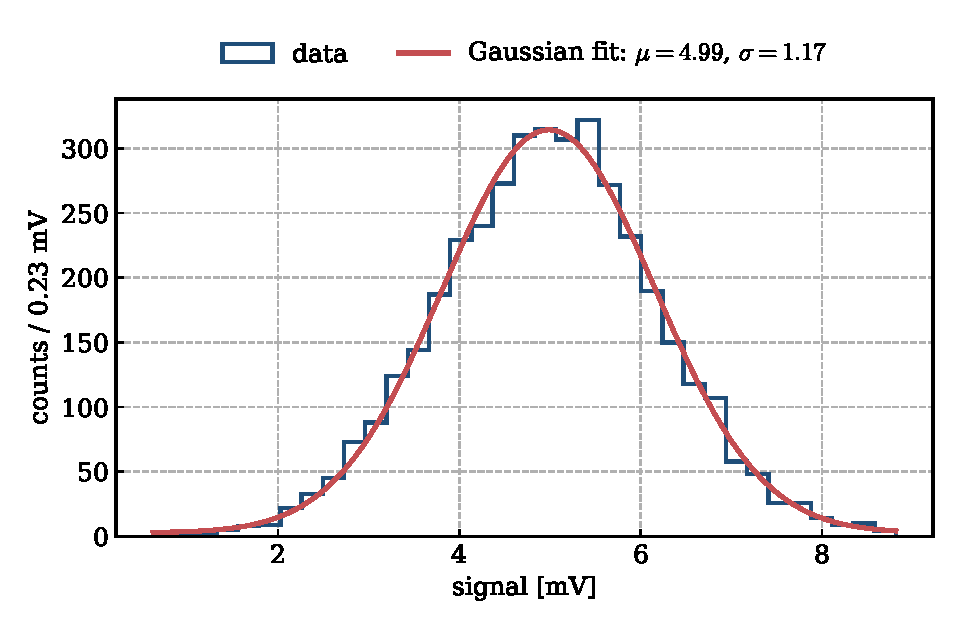
\includegraphics[width=0.72\linewidth]{histfit_module_example.pdf}
\caption{\code{save\_histogram\_with\_fit()} の出力例。ヒストグラムは乱数シード 42 で生成した 4000 個の信号値、実線はガウス関数によるフィットを表す。}
\label{fig:histfit-module-example}
\end{figure}

\code{fit\_model} には、あらかじめ登録した名前だけでなく、同じ呼び出し規約を持つ自作関数も渡せる。指数分布から生成したデータのヒストグラムへ、指数減衰関数を当てはめる例を次に示す。

\begin{lstlisting}[language=Python]
import numpy as np

from histfit_tools import save_histogram_with_fit


def exponential_decay(
    x: np.ndarray,
    amplitude: float,
    tau: float,
    offset: float,
) -> np.ndarray:
    return amplitude * np.exp(-x / tau) + offset


rng = np.random.default_rng(42)
decay_data = rng.exponential(scale=3.0, size=4000)

save_histogram_with_fit(
    decay_data,
    "figures/custom_fit.png",
    bin_width=0.25,
    data_range=(0.0, 15.0),
    fit_model=exponential_decay,
    p0=[300.0, 3.0, 0.0],
)
\end{lstlisting}

\code{fit\_model} は、登録済みのモデル名に加えて、同じ呼び出し規約を持つ callable を受け取る。これにより、パッケージ本体を変更せずに利用者定義のモデルを渡せる。

\section{docstring、型ヒント、README}

自作モジュールには、入力、返り値、例外条件、導入方法を記述する必要がある。関数単位の情報は docstring と型ヒント、パッケージ全体の情報は README が担う。

\subsection{docstring と型ヒント}

docstring\index{docstring@docstring|textbf} には、引数の意味と既定値、返り値、例外条件を記述する。\code{help()} と、docstring 表示に対応したエディタの補完機能は、この情報を参照する。

\code{save\_histogram\_with\_fit} には、\code{data: ArrayLike}、\code{output\_path: str | Path}、\code{fit: bool = True} のような型ヒント\index{かたひんと@型ヒント|textbf}が付いている。VS Code などのエディタでは、関数名にカーソルを合わせたときや補完候補を開いたときに、これらの型ヒントと docstring の先頭が表示されることが多い。したがって、docstring は文書であると同時に、コーディング中に参照できる説明でもある。

docstring の第 1 行には、関数の役割を一文で記述する。たとえば「ヒストグラムと誤差棒を描き、必要ならフィット線も重ねて保存する。」と書き、その後に引数、返り値、例外条件を続ける。

\subsection{README に書くべきこと}

\code{README.md} には、パッケージ全体の目的と導入方法を記述する。この例では次の 4 点を含める。

\begin{itemize}
\item このパッケージが何をするか
\item どうインストールするか
\item 最小の使用例
\item 主要な依存関係
\end{itemize}

たとえば最小限の README は次のようになる。

\begin{lstlisting}[numbers=none, xleftmargin=2\zw, title={README.md}]
# histfit_tools

Histogram plotting and fitting utilities for analysis scripts.

## Installation

```bash
uv pip install .
```

## Example

```python
from histfit_tools import save_histogram_with_fit
```
\end{lstlisting}

README はパッケージ全体の目的、導入方法、最小使用例を示し、docstring は関数単位の入出力契約を示す。両者の対象範囲を分け、同じ情報を重複して保守しない。

\section{\code{uv pip} による通常インストールと editable install}

\subsection{通常インストール}

現在のプロジェクト用仮想環境へパッケージを通常インストールするには、パッケージのルートディレクトリで \code{uv pip install .}\index{pip@\code{pip}!install@\code{install}|textbf} を実行する。\code{uv pip} は pip 互換のインターフェースであり、仮想環境内に \code{pip} コマンドがインストールされていない場合にも利用できる。

\begin{lstlisting}[numbers=none, xleftmargin=2\zw]
$ uv pip install .
\end{lstlisting}

これは現在のソースからビルドしたパッケージを環境へインストールする操作である。後から \code{src/histfit\_tools/plotting.py} を編集しても、その変更はインストール済みのパッケージへ自動では反映されない。変更後に \code{uv pip install .} を再実行する。

\subsection{editable install}
\index{editable install@editable install|textbf}

開発中は、\code{uv pip install -e .}\index{pip@\code{pip}!install -e@\code{install -e}|textbf} による editable install を利用できる。

\begin{lstlisting}[numbers=none, xleftmargin=2\zw]
$ uv pip install -e .
\end{lstlisting}

\code{-e} は editable の略であり、インストール先から手元のソースディレクトリを参照できる形でパッケージを登録する。したがって、Python ソースの変更を再インストールせずに import 側へ反映できる。関数定義や docstring を反復して変更する開発環境で用いる。

ただし、editable install が自動的に反映する範囲は、ビルドバックエンドと変更内容に依存する。\code{pyproject.toml} の依存関係を変更した場合や、後述する pybind11 のような C++ 拡張を編集した場合には、環境の同期、再インストール、再ビルドが必要になる。

\subsection{インストール確認}

インストール後は、短い import テストでパッケージを読み込めることを確認する。

\begin{lstlisting}[numbers=none, xleftmargin=2\zw]
$ uv run python -c "from histfit_tools import save_histogram_with_fit; print(save_histogram_with_fit)"
\end{lstlisting}

この import テストは、パッケージ名と公開関数を解決できることを確認する。依存関係、計算、ファイル出力を含む動作は、既知の小規模入力で関数を実行し、戻り値と保存ファイルを検証する統合テストで確認する。

\section{Git リポジトリによるパッケージの共有}

研究室内や共同研究で共有する場合は、Git リポジトリによってソース、テスト、設定の変更履歴を管理できる。\code{uv init --lib} は、外側に既存の Git リポジトリがなく、\code{--vcs none} も指定していなければ、初期化対象に \code{.git/} を作る。

GitHub\index{github@GitHub|textbf} で共有する場合は、GitHub の Web 画面でコミットを持たない空のリポジトリを作る。リポジトリ名と公開範囲を指定し、手元にある README と \code{.gitignore} は GitHub 側で重複して作成しない。

空のリモートリポジトリを作成した後、記録対象を確認して次のコマンドを実行する。

\begin{lstlisting}[numbers=none, xleftmargin=2\zw]
$ git add pyproject.toml uv.lock README.md src tests .python-version
$ git commit -m "Create histfit_tools package"
$ git remote add origin git@github.com:username/histfit_tools.git
$ git push -u origin main
\end{lstlisting}

\code{uv init --vcs none} のように Git 初期化を明示的に無効化して始めた場合には、最初に \code{git init} が必要になる。

\code{.venv/} や \code{\_\_pycache\_\_/} を追跡対象から除外する規則は、\code{.gitignore} に記述する。Git の状態確認、ステージング、コミット、リモート接続は付録~\ref{app:git} で扱う。

GitHub などに置いたリポジトリを別環境から直接インストールするコマンドは、次のとおりである。

\begin{lstlisting}[numbers=none, xleftmargin=2\zw]
$ uv pip install "git+ssh://git@github.com/username/histfit_tools.git"
\end{lstlisting}

タグやコミットを固定したいなら、URL の末尾に \code{@v0.1.0} や \code{@9f3c1a2} を付ける。

\begin{lstlisting}[numbers=none, xleftmargin=2\zw]
$ uv pip install "git+ssh://git@github.com/username/histfit_tools.git@v0.1.0"
\end{lstlisting}

タグまたはコミットハッシュを URL に含めると、後日の再インストールでも同じリビジョンを指定できる。研究ノートには、インストールに用いた URL とリビジョンを記録する。

\section{実行時依存関係と開発用依存関係}

依存関係は、利用者に必要な実行時依存関係、開発者だけが使う開発用依存関係、開発・検証環境を再現するロックファイルの三つに分ける。

\begin{description}
\item[実行時依存関係] パッケージを import して使うだけで必要なもの。今回なら \code{numpy}、\code{matplotlib}、\code{scipy} がこれに当たる。
\item[開発用依存関係] テスト、整形、静的解析にだけ必要なもの。今回なら \code{pytest} や \code{ruff} がこれに当たる。
\item[ローカル環境の固定] 開発者どうしで完全に同じ環境を再現したいときの情報。これは \code{uv.lock} が担う。
\end{description}

ライブラリの \code{dependencies} には、実装とテストによって確認した互換範囲を記述する。根拠なく \code{numpy==2.0.0} のような完全固定を行うと、利用者側の他の依存関係と両立しない場合がある。下限だけを検証した場合は \code{numpy>=2.0} のように記述し、非互換の上限が判明している場合はその上限も記述する。リポジトリ内の開発・検証環境は \code{uv.lock} で再現する。

開発中には、Jupyter、Sphinx、mkdocs など、利用者には不要でも開発者には必要な道具が増える。これらをすべて実行時依存関係へ含めると、利用者のインストール量と依存関係の衝突リスクが増す。公開 API と実行時依存関係は必要最小限に保ち、開発用の道具は開発用依存関係へ分ける。

\section{解析パッケージの作成と検証}

\begin{enumerate}
\item \textbf{最小パッケージの作成}。
空の作業ディレクトリで \code{uv init --lib signal\_tools} を実行し、生成された \code{pyproject.toml} と \code{src/signal\_tools/\_\_init\_\_.py} を確認せよ。\code{--lib} を付けた理由、\code{src} レイアウトで未インストールの作業ツリーを誤って import する問題を検出しやすい理由、\code{pyproject.toml} の \code{name} と \code{requires-python} の意味を説明せよ。

\item \textbf{公開関数とテストの追加}。
\code{src/signal\_tools/statistics.py} に、数値列を受け取って算術平均を返す \code{mean\_signal(values)} を作れ。空列では \code{ValueError} を送出せよ。\code{\_\_init\_\_.py} から再公開し、\code{from signal\_tools import mean\_signal} で呼び出せる状態にせよ。\code{tests/test\_statistics.py} に通常入力と空入力のテストを書き、\code{uv run pytest} の末尾で \code{2 passed} と表示されることを確認せよ。

\item \textbf{引数、返り値、例外の文書化}。
\code{mean\_signal()} に型ヒントと複数行 docstring を追加し、\verb|uv run python -c "from signal_tools import mean_signal; help(mean_signal)"| で表示せよ。docstring の要約、引数、返り値、例外条件がそれぞれどの行に表示されたかを確認せよ。

\item \textbf{通常インストールと editable install の比較}。
別の仮想環境を 2 つ作り、一方では \code{uv pip install .}、もう一方では \code{uv pip install -e .} を実行せよ。インストール後に関数の戻り値を変更し、どちらの環境で変更が直ちに反映されるかを確認せよ。\code{-e} はソースディレクトリを参照可能な形で登録する指定であり、依存関係の解決やビルド処理をすべて省略する指定ではない。

\item \textbf{依存関係と生成物の分類}。
NumPy を実行時依存関係、pytest と ruff を開発用依存関係として追加し、\code{pyproject.toml} の該当箇所を示せ。さらに \code{.gitignore} に \code{.venv/}、\code{\_\_pycache\_\_/}、\code{.pytest\_cache/}、\code{dist/} を書き、\code{git status --short} にこれらが現れないことを確認せよ。\code{uv.lock} をコミットするかどうかはプロジェクトの運用方針によるため、本課題では自分の判断と理由を記述せよ。
\end{enumerate}

自作モジュールによって処理を独立した関数へ分けると、各関数の正しさと処理時間を個別に調べられる。次章では、この構造を利用してボトルネックを測定し、計算量、配列演算、メモリ使用量、逐次処理の観点から実装を改善する。

\chapter{Python 解析の高速化}
\label{chap:performance}

\section{処理時間の基準測定}

高速化\index{こうそくか@高速化|textbf}を始める前に、どこが遅いのかを測る。読込みが遅いのか、探索が遅いのか、図の作成が遅いのかを区別しないまま最適化しても、効果は見えにくい。

ここで役立つのが \code{time.perf\_counter}\index{perf_counter@\code{time.perf\_counter}|textbf} である。処理の前後で時刻を取り、差を記録するだけでも、どの段階が重いかの見当が付く。大切なのは、全体時間だけでなく、読込み、前処理、探索、書き出し、作図のように段階を分けて測ることである。

\begin{lstlisting}[language=Python]
import time

t0 = time.perf_counter()
run_analysis()
t1 = time.perf_counter()
print(f"elapsed = {t1 - t0:.3f} s")
\end{lstlisting}

測定するときは、一度だけの結果を絶対視しないことも重要である。キャッシュや OS の状態で多少は揺れるため、条件をそろえ、複数回の傾向を見る方がよい。

\subsection{Jupyter の \code{\%timeit} による計測}

ノートブック環境で短い式や関数の速度を見たいときは、Jupyter の \code{\%timeit}\index{timeit@\code{\%timeit}|textbf} や \code{\%\%timeit} も便利である。複数回の実行を自動で繰り返し、平均的な実行時間を表示してくれるため、小さな差を見たいときに役立つ。

\begin{lstlisting}[language=Python]
%%timeit
result = array * 2
\end{lstlisting}

ただし、\code{\%timeit} はノートブックや IPython での簡便な測定であり、スクリプト全体の読込みや入出力を含めた時間を見るには向かない。小さな部品には \code{\%timeit}、解析全体には \code{perf\_counter} というように使い分けると整理しやすい。

\section{計算量の見積もり}
\index{けいさんりょう@計算量|textbf}
\index{あるごりずむ@アルゴリズム|textbf}

高速化では、実測だけでなく理屈の見積もりも役に立つ。入力サイズを $N$ としたとき、処理回数が $N$ に比例するのか、$N \log N$ 程度なのか、$N^2$ なのかで、大きなデータに対する伸び方がまるで違う。

厳密な漸近解析までできなくても、「データを 2 倍にしたら計算量は何倍くらいになるか」を考えるだけで十分に有益である。高速化はテクニック集ではなく、問題の構造を考える作業である。

変数名を短くしたり、関数を減らしたりしても、通常は実行時間にほとんど影響しない。一方、比較回数の削減、探索範囲の限定、配列演算への置換は、計算量または定数倍の処理時間を変え得る。

\subsection{オーダーとは何か}

ここでいう「オーダー」とは、入力サイズ $N$ を大きくしたときに処理回数がどのように増えるかを表す粗い記法である。通常は Big-O 記法\index{big-o@Big-O 記法|textbf}で書き、定数倍や低次の項を落として、最終的に支配的になる項だけを見る。

\[
3N + 20 \rightarrow O(N), \qquad
5N \log N + 100N \rightarrow O(N \log N), \qquad
N^2 + N \rightarrow O(N^2)
\]

よく出るオーダーには、たとえば次のようなものがある。

\begin{itemize}
\item $O(\log N)$: 範囲を半分ずつ絞る処理。二分探索など
\item $O(N)$: 1 回走査する処理。総和、平均、閾値判定、隣接差分など
\item $O(N \log N)$: ソートを含む処理。高速なソート、ソート後の探索など
\item $O(N^2)$: 全組合せ比較。全ペアの力ずく比較など
\end{itemize}

たとえば $N = 10^6$ なら、$\log_2 N$ はおよそ 20、$N \log_2 N$ はおよそ $2 \times 10^7$、$N^2$ は $10^{12}$ である。どちらも「増える」ことに変わりはないが、その増え方の差は圧倒的である。小さなテストデータでは目立たなくても、大きな入力では急に効いてくる。

ただし、オーダーは定数倍を完全に無視してよい、という意味ではない。同じ $O(N)$ でも 10 倍、100 倍の速度差が付くことは普通にある。ここでいう「ファクター」とは、この定数倍の差のことである。したがって、まずオーダーを疑い、その後で定数倍を詰める、という順序で考えると整理しやすい。

この中で、$O(\log N)$ や $O(N \log N)$ は初学者には直感を持ちにくい。そこで、まず二分探索で $O(\log N)$ を見てから、ソートで $O(N \log N)$ を見る。

\subsubsection{二分探索ではなぜ \texorpdfstring{$O(\log N)$}{O(log N)} になるか}

\(\log N\) は、「問題の大きさを毎回半分にできる」場面で現れる。たとえば昇順に並んだ列から目的の値を探す二分探索では、中央を見て、左半分か右半分のどちらかを捨てられる。

\begin{lstlisting}[language=Python]
def binary_search(values, target):
    left = 0
    right = len(values) - 1

    while left <= right:
        mid = (left + right) // 2
        if values[mid] == target:
            return mid
        if values[mid] < target:
            left = mid + 1
        else:
            right = mid - 1
    return -1
\end{lstlisting}

要素数が \(N\) 個あっても、1 回ごとに候補数が半分になるなら、必要な反復回数は \(N \to N/2 \to N/4 \to \cdots \to 1\) という形になる。これが \(\log_2 N\) 回程度である。したがって、二分探索は \(O(\log N)\) で動く。重要なのは、「1 個ずつ減らす」のではなく「毎回半分に減らす」ことが \(\log N\) を生む、という点である。

\subsubsection{ソートではなぜ \texorpdfstring{$O(N \log N)$}{O(N log N)} になるか}

ソートは、計算量の違いを理解するための基本例である。たとえば、挿入ソートやバブルソートのような初等的な方法は、一般に $O(N^2)$ で動く。一方、マージソートやヒープソートは $O(N \log N)$ であり、Python の \code{sorted()} も実用的な高速ソートを使っている。

ここで \(N \log N\) と書くなら、その意味も説明する必要がある。典型例であるマージソートでは、まず列を半分に分け、さらにその半分へ分ける、という分割を繰り返す。この分割の深さは、およそ \(\log_2 N\) 段である。一方、各段では、分かれた小列どうしを併合する過程で、全体として各要素を 1 回ずつ見るので \(O(N)\) かかる。

\[
\text{各段の仕事量 } O(N)
\quad \times \quad
\text{段数 } O(\log N)
\quad = \quad
O(N \log N)
\]

ここで重要なのは、「ソートは前処理にすぎない」と軽視しないことである。データを一度並べ替えるだけで、その後の探索や近傍判定がずっと安くなることがある。つまり、$O(N \log N)$ の前処理へ投資することで、後続の $O(N^2)$ を避けられるなら、全体として大幅に得をする。

データが 10 倍に増えたとき、$O(N^2)$ のソートはおおよそ 100 倍重くなるが、$O(N \log N)$ のソートは 10 倍強で済む。この差を理解しておくと、単にソートの名前を知るだけでなく、「なぜその方法を選ぶのか」を説明できるようになる。

\subsection{オーダーが改善する例: 重複判定}

問題をはっきりさせよう。長さ $N$ の整数列に、同じ値が 2 回以上現れるかを判定したいとする。

最も素朴な方法は、すべての組 $(i, j)$ を比べることである。

\begin{lstlisting}[language=Python]
def has_duplicate_slow(values):
    for i in range(len(values)):
        for j in range(i + 1, len(values)):
            if values[i] == values[j]:
                return True
    return False
\end{lstlisting}

この方法では、最悪の場合ほぼすべてのペアを比べるので $O(N^2)$ になる。データ量が 10 倍になると、比較回数はおおよそ 100 倍に増える。

しかし、いったんソートしてしまえば、同じ値どうしは必ず隣り合う。したがって、隣接要素だけを見れば重複を判定できる。

\begin{lstlisting}[language=Python]
def has_duplicate_fast(values):
    values_sorted = sorted(values)
    for i in range(len(values_sorted) - 1):
        if values_sorted[i] == values_sorted[i + 1]:
            return True
    return False
\end{lstlisting}

\code{sorted()} の部分は $O(N \log N)$、その後の 1 回走査は $O(N)$ なので、全体は $O(N \log N)$ である。元の $O(N^2)$ より明確に良い。ここで本質なのは、Python の書き方が少し変わったことではなく、「全比較」という問題の解き方をやめたことである。

Python の \code{set(values)} を使えば、重複判定は平均的に $O(N)$ で実行できる。ここでは、ソート後の走査によって処理量を減らす考え方を説明するため、ソートを用いた例を示している。

同じ考え方は探索でも現れる。未整列の列から目的の値を探す線形探索は $O(N)$ だが、整列済みの列なら二分探索で $O(\log N)$ にできる。したがって、「一度だけ探す」のか「何度も探す」のかによって、先にソートする価値があるかどうかも変わる。前処理に時間を使っても、その後の探索を何度も繰り返すなら、全体としては得になることが多い。

\subsection{オーダーは同じで定数倍だけ改善する例}

今度は、$N \times N$ 行列 $A$ が対称行列かどうか、すなわち $A_{ij} = A_{ji}$ が成り立つかを調べる問題を考える。

最も素朴な方法は、すべての $(i, j)$ について比較することである。

\begin{lstlisting}[language=Python]
def is_symmetric_slow(A):
    n = len(A)
    for i in range(n):
        for j in range(n):
            if A[i][j] != A[j][i]:
                return False
    return True
\end{lstlisting}

これは $n^2$ 回程度の比較を行うので $O(N^2)$ である。

しかし、対称性の判定では、上三角と下三角は同じ情報を二重に見ている。したがって、片側だけ見れば十分である。

\begin{lstlisting}[language=Python]
def is_symmetric_fast(A):
    n = len(A)
    for i in range(n):
        for j in range(i + 1, n):
            if A[i][j] != A[j][i]:
                return False
    return True
\end{lstlisting}

こちらもオーダーは同じく $O(N^2)$ だが、比較回数はおよそ $n(n-1)/2$ 回になり、素朴な実装のほぼ半分で済む。つまり、問題の大きさに対する増え方は変わっていないが、無駄な比較を消したことで定数倍が改善している。

この例は、「同じオーダーでも速くなる」ことを示している。図~\ref{fig:vectorization-benchmark} の隣接差分フィルタの比較も、基本的にはこの種類の改善である。比較回数そのものを 2 次から 1 次へ落としたのではなく、同じ種類の処理をより効率よく実装しているのである。

\section{ベクトル化・型・逐次処理による改善}

\subsection{NumPy と pandas による高速化}

アルゴリズムを見直した後は、NumPy や pandas へ処理を移すことで、Python レベルのループを減らせる。特に差分計算、ソート、列抽出、フィルタは、これらのライブラリが得意とする。図~\ref{fig:vectorization-benchmark} からも、ベクトル化\index{べくとるか@ベクトル化|textbf}が速度に与える効果を視覚的に確認できる。

ここで注意したいのは、NumPy や pandas を使えば自動的に何でも速くなるわけではないことである。根本的に無駄な比較をしているなら、配列演算へ移しても限界がある。まず計算量を減らし、そのうえで実装をベクトル化するという順序が自然である。

\subsection{メモリとコピーの管理}
\index{めもりかんり@メモリ管理|textbf}
\index{びゅー@ビュー|textbf}
\index{こぴー@コピー}

速度だけを見ていると、メモリ使用量が大きくなりすぎて逆に遅くなることがある。巨大な中間配列を何度も作る実装では、CPU よりもメモリ転送が支配的になる場合がある。

そのため、高速化では「何回ループしたか」だけでなく、「何回コピーしたか」も見る必要がある。不要なコピーを減らし、必要な列や範囲だけを扱う設計は、速度と安定性の両方に効く。

NumPy では、スライスが元配列とメモリを共有するビューになる一方、条件抽出は新しい配列を作る。次のコードで両者を確認できる。

\begin{lstlisting}[language=Python]
import numpy as np

values = np.arange(1_000_000, dtype=np.float64)
view = values[100:200]
copied = values[values % 2 == 0]

print(values.nbytes)
print(view.nbytes, np.shares_memory(values, view))
print(copied.nbytes, np.shares_memory(values, copied))
\end{lstlisting}

実行結果は次の通りである。

\begin{lstlisting}[numbers=none, xleftmargin=2\zw]
8000000
800 True
4000000 False
\end{lstlisting}

\code{nbytes} は配列要素が占めるバイト数を表す。\code{np.shares\_memory(a, b)} は 2 配列が同じメモリ領域を共有するかを調べる。この例では、\code{view} 自体が参照する要素は 800 バイト分だが、元配列のメモリを共有するため、\code{view} の要素を書き換えると対応する \code{values} の要素も変わる。\code{copied} は 50 万要素の独立した配列であり、新たに 4 MB を使う。なお、\code{nbytes} は Python オブジェクト自体の管理領域を含まないため、プロセス全体のメモリ使用量と完全には一致しない。

\subsection{分割読込み、並列化、ストリーミング}
\index{ぶんかつよみこみ@分割読込み|textbf}
\index{へいれつか@並列化|textbf}
\index{すとりーみんぐ@ストリーミング|textbf}

大規模解析では、全部を一度にメモリへ載せない設計も重要である。ファイル単位で処理し、必要な情報だけを持ち回る。さらに、独立な単位に分割できるなら並列化も検討できる。

ストリーミング処理では、「今必要な範囲だけを覚える」という考え方が中心になる。全履歴が不要なら保持しない、集計済みの量は逐次更新する、といった設計が有効である。メモリ節約と速度向上が同時に得られることも多い。

例えば、1 行に 1 個の測定値が書かれた \code{values.txt} の平均は、全行をリストへ保存せずに求められる。

\begin{lstlisting}[numbers=none, xleftmargin=2\zw, title={values.txt}]
1.5
2.0
4.0
2.5
\end{lstlisting}

\begin{lstlisting}[language=Python]
def streaming_mean(path):
    count = 0
    total = 0.0

    with open(path, "r", encoding="utf-8") as f:
        for line_number, line in enumerate(f, start=1):
            text = line.strip()
            if text == "":
                continue
            try:
                value = float(text)
            except ValueError as exc:
                raise ValueError(f"line {line_number}: {text!r}") from exc
            count += 1
            total += value

    if count == 0:
        raise ValueError("input contains no numeric values")
    return total / count


print(streaming_mean("values.txt"))
\end{lstlisting}

出力は \code{2.5} となる。引数 \code{path} は入力ファイルの場所であり、\code{enumerate(..., start=1)} はエラー箇所をファイルと同じ 1 始まりの行番号で報告するために使う。この関数が保持するのは現在行、件数、合計だけなので、入力行数が増えても集計用メモリはほぼ一定である。ただし、中央値や全体のソートのように全データの順序が必要な統計量は、この単純な方法だけでは正確に求められない。

\section{プロファイリングと低レベル実装}

\subsection{プロファイラによるボトルネックの特定}
\index{ぼとるねっく@ボトルネック|textbf}

本格的に遅い理由を調べるなら、プロファイラ\index{ぷろふぁいら@プロファイラ|textbf}も役立つ。例えば \code{cProfile}\index{cprofile@\code{cProfile}|textbf} を使うと、どの関数に時間が使われているかを確認できる。

\begin{lstlisting}[language=Python]
import cProfile

cProfile.run("run_analysis()", sort="cumtime")
\end{lstlisting}

ただし、プロファイラの数字も文脈なしには読めない。回数が多いから遅いのか、1 回が重いのか、入出力を待っているのかを区別する必要がある。測定値とコード構造を一緒に見ることが重要である。

\begin{lstlisting}[numbers=none, xleftmargin=2\zw]
ncalls  tottime  cumtime  function
100000   1.25     1.40    check_pair
    10   0.02     2.10    read_all_files
\end{lstlisting}

この結果例では、\code{check\_pair} は 1 回は軽いが回数が多く、\code{read\_all\_files} は内部の処理込みで累積時間が大きいと読める。どの列が何を意味するかを理解すると、改善方針が立てやすくなる。

\subsection{C や C++ へ書き換えるという選択肢}

Python は開発速度が高いが、計算コアのすべてを Python で書く必要はない。アルゴリズムを十分に整理したうえで、どうしても重い部分だけを C や C++ へ移す、というのは自然な選択肢である。

ただし、言語を変える前に Python 側で何が遅いかを把握しておく必要がある。ボトルネックが入出力や高水準の設計にあるなら、C++ 化しても大きな改善にならない。低レベル言語への移行は、最後の切り札として考える方がよい。

\begin{lstlisting}[language=C++]
for (std::size_t i = 0; i < n; ++i) {
    for (std::size_t j = i + 1; j < n; ++j) {
        if (std::abs(times[j] - times[i]) <= window) {
            ++count;
        }
    }
}
\end{lstlisting}

この書き換えは、定数倍の改善をもたらすことがある。しかし、比較回数そのものが多すぎるなら本質的な改善ではない。アルゴリズムと実装言語を分けて考える姿勢が必要である。

\subsection{Python からの C/C++ コード呼び出し}
\index{cython@Cython|textbf}
\index{pybind11@pybind11|textbf}

方法はいくつかある。たとえば \code{ctypes} で共有ライブラリを呼ぶ方法、Python C 拡張を書く方法、pybind11 を使って C++ を Python から自然に使える形へ包む方法などがある。さらに、Python と C の中間に位置する Cython を使い、Python に近い構文のまま重いループだけをコンパイルする方法も、この節に含まれる重要な選択肢である。

\begin{lstlisting}[language=Python]
cdef int i
cdef double total = 0.0

for i in range(n):
    total += values[i]
\end{lstlisting}

ここで \code{cdef} は Cython 特有の宣言であり、変数を Python オブジェクトではなく C の整数や浮動小数点数として扱わせるために使う。これにより、ループ内部の型判定やボックス化のコストを減らせる。

どの方法を選ぶかは、必要な速度、保守性、ビルドの難しさで決まる。目安としては次のように考えるとよい。

\begin{itemize}
\item \code{ctypes}: 既にある C の共有ライブラリを手早く呼びたいときに向く。設定は比較的軽いが、引数や戻り値の型を手で合わせる必要がある
\item Python C 拡張: Python 本体の C API を直接使う最も低レベルな方法で、自由度は高いが記述量も多い
\item \code{pybind11}: C++ の関数やクラスを Python から自然に使える形で公開しやすい。C++ 側の実装をすでに持っている場合に相性がよい
\item Cython: Python に近い構文を保ちながら、重いループや数値計算だけへ型を付けてコンパイルしたいときに向く
\end{itemize}

短い試作なら \code{ctypes}、Python らしい使い勝手まで整えたいなら pybind11、既存の Python 風コードを保ちながら内側だけ速くしたいなら Cython、といった選択が考えられる。重要なのは、インタフェースを狭く保ち、重い部分だけを外へ出すことである。pybind11 の最小構成は付録~\ref{app:pybind11} を参照してほしい。

\begin{lstlisting}[language=Python]
result = fast_module.count_pairs(times, window)
\end{lstlisting}

Python 側の呼び出しが単純であれば、内部実装を後から差し替えやすい。まず Python で正しい API を決め、その内部だけを高速化するという順が自然である。なお、Cython も強力だが、アルゴリズムそのものが無駄な場合には決定打にならない。この点は C++ 化と同じであり、まず Python 側で何が遅いのか、どのループが本当に支配的なのかを見極めた後に使う方が効果的である。

\subsection{外部実装を参考にするときの見方}

高速化を学ぶときは、外部の C や C++ の実装例を読むことが参考になる。ただし、そこで大切なのは固有名詞を覚えることではない。まず見るべきなのは、どの問題を解いているのか、どのアルゴリズムを選んでいるのか、どの部分だけを低レベル言語へ移しているのか、という点である。

高速化の章では、このような例を参照しながら、次の二つを常に区別して考える。

\begin{itemize}
\item アルゴリズムを変えたから速くなったのか
\item 実装言語を変えたから速くなったのか
\end{itemize}

多くの場合、最初に効くのは前者である。

したがって、高速化のレポートを書くときは、「NumPy にした」「C++ にした」で終わらせない方がよい。何が変わった結果として速くなったのかを、計算量、比較回数、メモリ配置、ループの位置といった観点で説明するべきである。

\section{高速化前後の比較と測定条件の報告}

高速化の結果は、本文中で比較できる形に整理すると読みやすい。例えば、次は報告形式を示すための仮想的な数値例である。

\begin{lstlisting}[numbers=none, xleftmargin=2\zw]
slow version : 182.4 s
vectorized   :  12.7 s
streaming    :   4.8 s
\end{lstlisting}

実際の報告では、この形式へ自分で測定した値を入れる。この表現だけでは理由が分からないので、続けて「比較回数を減らした」「Python ループを配列演算へ移した」「全件保持をやめた」といった説明を添える。数値と理由の両方がそろって初めて報告になる。

特に、高速化の報告では「$O(N^2)$ から $O(N \log N)$ や $O(N)$ へ落とした改善」と、「同じ $O(N)$ や $O(N^2)$ のまま NumPy, Cython, C++ などで定数倍を詰めた改善」を分けて書くとよい。前者は問題の解き方を変えた改善であり、後者は実装の効率を上げた改善である。この二つを混同しない方が、読者にも自分にも何が効いたのかが伝わりやすい。

\begin{lstlisting}[language=Python]
import numpy as np

values = np.array(data, dtype=np.float64)
diffs = np.diff(values)
count = np.count_nonzero(diffs > 0.25)
\end{lstlisting}

\begin{figure}[tbp]
\centering
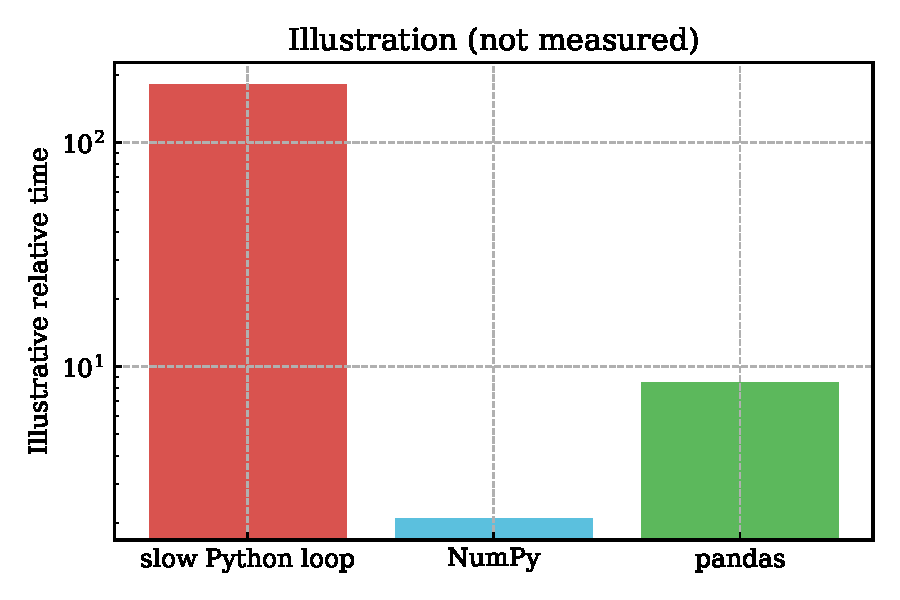
\includegraphics[width=0.82\linewidth]{vectorization_benchmark.pdf}
\caption{実行時間の比較方法を示す模式例。値は説明用であり、特定の計算機で得たベンチマーク結果ではない。縦軸には対数目盛を用いている。}
\label{fig:vectorization-benchmark}
\end{figure}

図~\ref{fig:vectorization-benchmark} は実行時間の大小を比較するための図であり、結果の正しさまでは保証しない。高速化の前後で同じ \code{count} が得られることをテストし、その上で入力サイズ、反復回数、実行環境、代表値をそろえて時間を比較する必要がある。

\section{処理時間・メモリ・プロファイルの測定演習}

\begin{enumerate}
\item \textbf{結果を保持したベクトル化}。
\verb|values = np.arange(1_000_000, dtype=np.float64)| について、各要素を二乗してから総和を求める処理を Python の \code{for} 文と NumPy の列演算で実装せよ。\code{np.isclose()} で結果が一致することを先に確認し、その後で \code{time.perf\_counter()} を使って各方法を 5 回ずつ測定せよ。最小値または中央値を報告し、1 回だけの値を比較しない理由を説明せよ。

\item \textbf{入力サイズと計算量の関係}。
本文の \code{has\_duplicate\_slow()} と \code{has\_duplicate\_fast()} を使い、重複を含まない入力について \(N=1000, 2000, 4000\) の実行時間を測定せよ。\(N\) を 2 倍にしたときの時間比を求め、\(O(N^2)\) と \(O(N\log N)\) の予想と比較せよ。計算機や実行時の状態によって時間は変わるため、絶対時間ではなく比と傾向を説明せよ。

\item \textbf{ビューとコピーの影響}。
本文の \code{values}、\code{view}、\code{copied} を作り、\code{view[0] = -1} と \code{copied[0] = -2} を実行した後で \code{values[100]} と \code{values[0]} を表示せよ。前者だけが変化する理由を、\code{np.shares\_memory()} の結果と対応させて説明せよ。さらに \code{float32} と \code{float64} で同じ要素数の \code{nbytes} を比較せよ。

\item \textbf{逐次集計の検証}。
1 から 100000 までを 1 行ずつ書いたファイルを作り、本文の \code{streaming\_mean()} で平均を求めよ。期待値は \code{50000.5} である。同じファイルを全件リストへ読み込む実装も作り、結果の一致を確認せよ。両者が保持するデータ量を、入力行数 \(N\) に対するオーダーで説明せよ。

\item \textbf{プロファイル結果に基づく改善対象の選定}。
自分の解析スクリプト、または 1 問目の 2 実装を関数へ分けたスクリプトを \code{python -m cProfile -s cumtime script.py} で測定せよ。出力の \code{ncalls}、\code{tottime}、\code{cumtime} の意味を説明し、累積時間の上位 3 関数を記録せよ。そのうち改善対象に選ぶ関数と、選ばない関数の理由をそれぞれ述べよ。
\end{enumerate}

性能改善は、速いコードを書くことだけを目的としない。高速化の前後で同じ結果が得られることを検証し、入力条件と測定方法を記録して初めて、改善を再現できる。次章では、同時観測イベントの探索を題材として、読込み、検証、可視化、フィット、性能測定を一つの解析へ統合する。

\chapter{課題: 同時観測イベントの探索}
\label{chap:kadai}
\index{どうじかんそく@同時観測|textbf}
\section{入力データと実行環境の準備}

この課題では、次のファイルを配布する。

\begin{itemize}
\item \code{events\_data.zip}
\item \code{slow\_event\_analysis.py}
\item 本テキスト
\end{itemize}

\code{events\_data.zip} を展開すると、\code{events\_data/} というディレクトリが得られる。日ごとに gzip 圧縮されたイベントファイルがあり、年・月ごとのディレクトリに分かれている。

課題のスクリプトやデータは、GitHub リポジトリ
（\url{https://github.com/i-komae/python_textbook}）
から入手できる。手元に配布物がそろっていない場合は、リポジトリの取得と、直下にある \code{slow\_event\_analysis.py} および \code{events\_data.zip} の配置確認が必要である。\code{events\_data.zip} の展開によって得られる \code{events\_data/} が入力ディレクトリとなる。

配布物は意図的に最小限にしてある。したがって、入力、正解判定の対象となるファイル、自分で実装する範囲を着手前に整理する必要がある。

\subsection{配布コードによる基準測定}

最初の基準測定では、配布されたコードを変更せずに実行せよ。

\begin{lstlisting}[numbers=none, xleftmargin=2\zw]
$ python3 slow_event_analysis.py events_data --outdir slow_output
\end{lstlisting}

全期間の処理時間は、データ量、ストレージ、計算機によって変わる。初回の対象は数日分とし、入力形式と出力の確認後に対象期間を広げるのがよい。

最初から完成版を書く必要はない。配布コードの処理時間と出力を変更前に記録しておけば、各修正の効果を基準値との比較によって説明できる。

\subsection{入力ファイルの構造}

解析を始める前に、gzip ファイルを一つ開き、各列の意味を確認せよ。

\begin{lstlisting}[numbers=none, xleftmargin=2\zw]
$ gzip -cd events_data/2024/01/events_2024_01_01.txt.gz | head
\end{lstlisting}

各行の列は次のようになっている。

\begin{lstlisting}[numbers=none, xleftmargin=2\zw]
event_id year month day hhmmss ns detector_id signal
\end{lstlisting}

各列の型と役割を言語化すると、整数として扱う列、時刻を構成する列、識別子としてのみ使う列、物理量として解釈する列を区別できる。この区別が曖昧なままでは、型変換や時刻比較の誤りを招く。

この課題では、2 事象の時刻差を ns 単位まで含めて評価し、\(\lvert \Delta t \rvert \le 250\,\mathrm{ns}\) を満たすものを「同時観測」と定義する。したがって、\code{hhmmss} 列だけを見ればよいわけではなく、\code{ns} 列も含めて時刻を一つの量として組み立てる必要がある。秒境界や日付境界をまたぐ場合にどう振る舞うかも、この定義を満たす形で確認しなければならない。
\index{じこくさ@時刻差|textbf}
\index{じかんまど@時間窓|textbf}

\subsection{小規模入力による検証}

500 日分の全データを処理する前に、数日分を別ディレクトリへコピーし、短時間で再実行できる検証用入力を用意せよ。

\begin{lstlisting}[numbers=none, xleftmargin=2\zw]
$ mkdir -p events_data_small/2024/01
$ cp events_data/2024/01/events_2024_01_01.txt.gz events_data_small/2024/01/
$ cp events_data/2024/01/events_2024_01_02.txt.gz events_data_small/2024/01/
$ cp events_data/2024/01/events_2024_01_03.txt.gz events_data_small/2024/01/
\end{lstlisting}

小さい入力での確認は、速度のためではなく、正しさを素早く確かめるためである。数十秒で終わる条件を作っておけば、修正してすぐ再実行できる。大きなデータを回すのは、その後で十分である。

\begin{lstlisting}[numbers=none, xleftmargin=2\zw]
n_pairs_total = 241
analysis_sec = 18.4
\end{lstlisting}

この段階では、数値そのものよりも、修正のたびに一貫した結果が出るかが大切である。件数が毎回変わる、出力ファイルの形式が揺れる、といった状態では、その先の高速化に進むべきではない。

\section{検証・修正・高速化の要件}

必須項目は次の五点である。

\begin{enumerate}
\item 配布コードの処理時間の測定
\item 同時観測イベント数の検証
\item バグの特定と修正
\item 解析処理の高速化
\item 同時観測イベントの時刻差分布の作図とフィット
\end{enumerate}

この順序にも意味がある。性能改善に着手するのは、元のコードの振る舞いを把握し、正しさを確認した後である。誤ったコードを高速化しても、誤った結果が速く得られるだけである。

\subsection{必須出力}

必須出力は次の三点である。

\begin{itemize}
\item 同時観測イベントの一覧
\item 同時観測イベントを構成する 2 事象の時刻差の分布
\item 同時観測イベントどうしの発生間隔、またはそれに相当する量の分布
\end{itemize}

ここでいう「2 事象の時刻差」は、同時観測と判定した 2 つのイベントの時刻差である。たとえば $\Delta t = t_2 - t_1$ と定義してよい。ただし、符号付きの値と絶対値のどちらを使うか、検出器番号によって向きをそろえるかを定め、その定義を明記せよ。

分布図には、ビン幅、横軸の範囲、単位を明記せよ。図だけを提示しても、量の定義と計数方法が不明では解釈できない。フィットを行う場合は、使用した範囲も記載せよ。

\begin{lstlisting}[numbers=none, xleftmargin=2\zw]
coincidence_pairs.csv
pair_dt_hist.pdf
pair_mean_gap_hist.pdf
summary.txt
\end{lstlisting}

ファイル名の流儀を最初に決めておくと、後で解析を繰り返したときにも混乱しにくい。どのファイルが一覧で、どれが図で、どれが数値要約なのかが名前から分かるようにしておくとよい。

\subsection{正しさを検証する基準値}
\index{ただしさのけんしょう@正しさの検証|textbf}

今回の配布データは 500 日分であり、正しく同時観測イベントを拾えていれば、全期間で得られる同時観測イベント数は

\begin{lstlisting}[numbers=none, xleftmargin=2\zw]
n_pairs_total = 12033
\end{lstlisting}

になる。この値が最終確認の目安である。

ただし、この値に合ったからといって、それだけで実装が正しいとは限らない。偶然件数だけ一致している可能性もある。実装の検証には、可能な範囲で個々のイベント対の内容と、ファイル境界付近の振る舞いも含める必要がある。

\begin{lstlisting}[numbers=none, xleftmargin=2\zw]
n_pairs_total = 12033
analysis_sec = 248.6
plot_sec = 1.8
\end{lstlisting}

このような要約ファイルを出しておくと、コード変更のたびに結果を比較しやすい。件数だけでなく処理時間も同じ場所へ残すと、正しさと速度を一緒に追える。

\section{提出レポートと発展的実装}

提出物は次の二つである。

\begin{itemize}
\item 解析に使った Python コード
\item LaTeX で書いたレポートと、その PDF
\end{itemize}

レポートには、少なくとも次の内容を含めよ。

\begin{itemize}
\item 元のコードの問題点
\item 正しさをどう検証したか
\item バグをどう修正したか
\item どう高速化したか
\item 改善前後の処理時間
\item 作成した図
\item フィット結果とその解釈
\end{itemize}

レポートの構成は、変更点の羅列ではなく、問題の発見、原因の切り分け、修正方針、検証方法、結果、考察の順が望ましい。図表は本文から参照し、その内容と解釈を説明せよ。

\begin{lstlisting}[numbers=none, xleftmargin=2\zw]
1. 元のコードの観察
2. バグの特定
3. 修正内容
4. 高速化方針
5. 結果の比較
6. 図とフィットの考察
\end{lstlisting}

この順序で書けば、読者は「何が問題で、どう直して、何が改善したのか」を追いやすい。レポートは成果物であると同時に、思考過程の記録でもある。

\subsection{発展課題}
\index{べんちまーく@ベンチマーク}

余裕があれば、図の作成やフィットまで含めた全体処理をさらに高速化してよい。さらに、NumPy や pandas を使うだけでなく、自分でアルゴリズムを設計し直したり、C や C++ で計算コアを実装したりしてもよい。

この発展課題では、特定の解法を要求しない。pandas を深く使う方向もあれば、ストリーミング処理を突き詰める方向もあり得るし、重い部分だけを別言語へ切り出す方向もあり得る。重要なのは、自分の方針を説明できることである。


\appendix
\chapter{SSH, 鍵認証, ファイル転送}
\label{app:ssh}
\index{ssh@SSH|textbf}
\index{かぎにんしょう@鍵認証|textbf}

\section{サーバーへの SSH 接続と鍵認証}

SSH（Secure Shell）は、離れた計算機との通信を暗号化し、その計算機上でコマンドを実行するための仕組みである。研究室や計算サーバーに接続し、大規模なデータ処理や長時間ジョブを実行する場合に利用する。GitHub への SSH 接続も同じ認証方式を用いるが、GitHub は対話的なシェルの接続先ではなく、Git 操作の認証先である。

\subsection{サーバーへの接続}

初回の SSH 接続では、接続先のホスト鍵の指紋（fingerprint）を確認することがある。これは接続先サーバーを識別するためのもので、自分の認証用公開鍵とは異なる。管理者など信頼できる経路から得た指紋と照合して登録する。ホスト鍵が変わったという警告では、再構築などの理由を確認してから更新する。詳細は OpenSSH の資料~\cite{openssh_manual} を参照する。
\index{ssh command@\code{ssh}|textbf}

最も基本的な形は次である。

\begin{lstlisting}[numbers=none, xleftmargin=2\zw]
$ ssh user@server.example.jp
\end{lstlisting}

\code{user} はサーバー上の自分のユーザー名、\code{server.example.jp} はホスト名である。ポート番号が既定の 22 でないなら \code{-p} を付ける。

\begin{lstlisting}[numbers=none, xleftmargin=2\zw]
$ ssh -p 2222 user@server.example.jp
\end{lstlisting}

接続後に入力したコマンドは、原則として接続先の計算機上で実行される。表示されるファイルも接続先にあるため、ローカルファイルとの取り違えは意図しない変更や削除につながる。作業を始める前に \code{hostname}、\code{whoami}、\code{pwd} を実行すれば、接続先、利用者名、作業ディレクトリを確認できる。

\subsection{SSH 鍵の作成}
\index{ssh-keygen@\code{ssh-keygen}|textbf}
\index{こうかいかぎ@公開鍵|textbf}
\index{ひみつかぎ@秘密鍵|textbf}

公開鍵認証では、公開鍵と秘密鍵の対を使用する。公開鍵をサーバーへ登録し、秘密鍵は接続元の計算機から外部へ渡さない。

\begin{lstlisting}[numbers=none, xleftmargin=2\zw]
$ ssh-keygen -t ed25519 -C "your_email@example.com"
\end{lstlisting}

既定の保存先を選ぶと、\code{\textasciitilde/.ssh/id\_ed25519} が秘密鍵、\code{\textasciitilde/.ssh/id\_ed25519.pub} が公開鍵になる。サーバーへ登録するのは \code{.pub} が付いた公開鍵だけである。\code{.pub} が付かない秘密鍵は共有しない。

\begin{lstlisting}[numbers=none, xleftmargin=2\zw]
$ ls -l ~/.ssh
\end{lstlisting}

秘密鍵の権限が緩いと SSH が拒否することがある。その場合は次のように直す。

\begin{lstlisting}[numbers=none, xleftmargin=2\zw]
$ chmod 700 ~/.ssh
$ chmod 600 ~/.ssh/id_ed25519
$ chmod 644 ~/.ssh/id_ed25519.pub
\end{lstlisting}

\subsection{サーバーへの公開鍵登録}
\index{ssh-copy-id@\code{ssh-copy-id}|textbf}

\code{ssh-copy-id} は、公開鍵を接続先の \code{authorized\_keys} へ追加するコマンドである。

\begin{lstlisting}[numbers=none, xleftmargin=2\zw]
$ ssh-copy-id user@server.example.jp
\end{lstlisting}

特定の公開鍵を使いたいなら \code{-i} で指定できる。

\begin{lstlisting}[numbers=none, xleftmargin=2\zw]
$ ssh-copy-id -i ~/.ssh/id_ed25519.pub user@server.example.jp
\end{lstlisting}

\code{ssh-copy-id} は、指定した公開鍵をサーバー側の \code{\textasciitilde/.ssh/authorized\_keys} へ追加する。公開鍵の転送と追記を一つのコマンドで実行できる。

\subsubsection{\code{ssh-copy-id} が使えない場合}

\code{ssh-copy-id} が使えない環境では、公開鍵を手動で登録する。登録対象は、次のコマンドで表示される 1 行全体である。

\begin{lstlisting}[numbers=none, xleftmargin=2\zw]
$ cat ~/.ssh/id_ed25519.pub
\end{lstlisting}

表示された 1 行全体を、サーバー側の \code{\textasciitilde/.ssh/authorized\_keys} へ追記する。サーバーへ通常のパスワードログインができるなら、自分でログインして追記してもよい。

\subsection{\code{ssh-agent} による秘密鍵の管理}
\index{ssh-agent@\code{ssh-agent}|textbf}

パスフレーズ付きの鍵を使う場合は、\code{ssh-agent} に読み込ませておくと毎回の入力を減らせる。

\begin{lstlisting}[numbers=none, xleftmargin=2\zw]
$ eval "$(ssh-agent -s)"
$ ssh-add ~/.ssh/id_ed25519
\end{lstlisting}

\section{接続設定と GitHub 連携}

\subsection{\code{\textasciitilde/.ssh/config} による接続設定}
\index{ssh config@\code{\textasciitilde/.ssh/config}|textbf}

\code{\textasciitilde/.ssh/config} には、接続先ごとのホスト名、利用者名、ポート番号、秘密鍵ファイルを記録できる。次の設定では、これらの接続条件に \code{labserver} という名前を付ける。

\begin{lstlisting}[numbers=none, xleftmargin=2\zw, title={\textasciitilde/.ssh/config}]
Host labserver
    HostName server.example.jp
    User student
    Port 2222
    IdentityFile ~/.ssh/id_ed25519
\end{lstlisting}

この設定を保存すると、次のコマンドが同じ接続条件を参照する。

\begin{lstlisting}[numbers=none, xleftmargin=2\zw]
$ ssh labserver
\end{lstlisting}

この設定ファイルには接続先、利用者名、秘密鍵ファイルの場所が記録されるが、秘密鍵そのものは含まれない。ただし、第三者による書き換えを防ぐため、所有者だけが読み書きできる権限を設定する。

\begin{lstlisting}[numbers=none, xleftmargin=2\zw]
$ chmod 600 ~/.ssh/config
\end{lstlisting}

\subsection{GitHub への SSH 鍵登録}

通常のサーバーとは違って、GitHub には \code{ssh-copy-id} を使わない。GitHub はシェル接続先ではなく、アカウント設定に公開鍵を登録する相手だからである。

GitHub の設定画面にある \code{SSH and GPG keys} へ公開鍵を登録する。GitHub CLI \code{gh} を使う場合は、認証手順の中で既存鍵の登録または新規鍵の作成を選択できる。

\begin{lstlisting}[numbers=none, xleftmargin=2\zw]
$ gh auth login --git-protocol ssh --web
\end{lstlisting}

GitHub CLI を使う場合は、既存の鍵を検出してアップロードするか、新しい鍵を作るかを対話的に選べる。GitHub CLI を使わない場合は、\code{cat ~/.ssh/id\_ed25519.pub} で表示した公開鍵を Web 画面へ貼り付ければよい。

\section{\code{scp}・\code{rsync} によるファイル転送}

\code{scp} は指定したファイルまたはディレクトリを転送する。\code{rsync} は送信元と転送先の差分を調べ、除外条件や中断後の部分ファイルの保持を指定できる。単発の転送には \code{scp}、同じディレクトリの反復同期には \code{rsync} を用いる。

\subsection{\code{scp} の最小例}
\index{scp@\code{scp}|textbf}

\code{scp} では、ローカルとリモートのどちらを送信元に書くかによって転送方向が決まる。両方向の最小例を次に示す。

\begin{lstlisting}[numbers=none, xleftmargin=2\zw]
$ scp result.csv user@server.example.jp:~/work/
$ scp user@server.example.jp:~/work/result.csv .
\end{lstlisting}

1 行目はローカルからサーバーへ送信し、2 行目はサーバーからローカルへ受信する。ディレクトリ全体を転送する場合は \code{-r} を付ける。

\subsection{差分同期に \code{rsync} を用いる理由}
\index{rsync@\code{rsync}|textbf}

\code{rsync} は、送信元と転送先の差分を転送し、\code{--partial} で中断時の部分ファイルを保持し、\code{--exclude} で転送対象を除外できる。解析用ディレクトリやコード一式を反復同期する場合は、変更のないファイルも再転送する \code{scp} より転送量を抑えられる。

\begin{lstlisting}[numbers=none, xleftmargin=2\zw]
$ rsync -aP ./analysis/ user@server.example.jp:~/work/analysis/
\end{lstlisting}

主なオプションの意味を次に示す。

\begin{description}
\item[\code{-a}] アーカイブ（archive）モードである。再帰コピーを行い、時刻や権限などもまとめて保つ。
\item[\code{-P}] \code{--partial --progress} の省略形である。途中ファイルを残しつつ進捗を表示する。
\item[\code{-v}] 何を転送しているか詳しく表示する。
\item[\code{-z}] 転送時に圧縮する。低速回線では有利だが、既に圧縮済みの大きなデータでは効果が薄いこともある。
\item[\code{--exclude}] 特定のファイルやディレクトリを転送対象から除外する。
\end{description}

次の例では、アーカイブモードと進捗表示を有効にし、転送先で再作成できる仮想環境、キャッシュ、ビルド成果物を除外する。

\begin{lstlisting}[numbers=none, xleftmargin=2\zw]
$ rsync -aPv \
  --exclude='.venv/' \
  --exclude='__pycache__/' \
  --exclude='build/' \
  --exclude='.mypy_cache/' \
  ./analysis/ user@server.example.jp:~/work/analysis/
\end{lstlisting}

この例では、依存関係の定義やソースコードから転送先で再生成できる仮想環境、キャッシュ、ビルド成果物を除外し、転送量を減らしている。

\subsubsection{末尾のスラッシュによる転送結果の違い}
\index{rsync@\code{rsync}!まつびのすらっしゅ@末尾のスラッシュ}

\code{rsync} では、送信元パスの末尾に \code{/} を付けるかどうかで意味が変わる。

\begin{lstlisting}[numbers=none, xleftmargin=2\zw]
$ rsync -aP analysis user@server:~/work/
$ rsync -aP analysis/ user@server:~/work/
\end{lstlisting}

1 行目は \code{analysis} というディレクトリごと送り、2 行目は \code{analysis} の中身を送る。末尾のスラッシュを取り違えると転送先の階層が 1 段ずれる。初回の転送前には、\code{--dry-run} を加えた実行で転送対象を確認できる。

転送条件やオプションの詳細は rsync の公式マニュアル~\cite{rsync_manual} で確認できる。

\chapter{Git と GitHub の基本}
\label{app:git}
\index{git@Git|textbf}
\index{github@GitHub|textbf}

\section{リポジトリ・ステージング・コミットの関係}

Git は、手元のファイルの変更履歴を記録するためのソフトウェアである。これに対して GitHub は、Git リポジトリを置いて共有するためのサービスである。

\begin{itemize}
\item Git: ローカルマシンでも単独で使えるバージョン管理システム
\item GitHub: Git リポジトリをホストし、共有、Issue、Pull Request などを提供するサービス
\end{itemize}

したがって、\code{git init}、\code{git add}、\code{git commit} は Git の話であり、GitHub 上のリポジトリを \code{clone} で取得したり、\code{push} で送ったりする段階で GitHub が関係する。

\subsection{リポジトリと公開範囲}
\index{りぽじとり@リポジトリ|textbf}
\index{こうかいはんい@公開範囲|textbf}

リポジトリは、コード、データ、履歴をまとめて管理する単位である。GitHub へ置く場合は、公開範囲も意識する必要がある。

\begin{itemize}
\item 公開（\code{public}）: 誰でも閲覧できる
\item 非公開（\code{private}）: 明示的に許可された利用者だけが閲覧できる
\item 内部（\code{internal}）: 主に GitHub Enterprise で、同じ Enterprise に属するメンバーへ公開する。単一の Organization 内だけに限定する設定とは異なる
\end{itemize}

授業用の配布物、研究中のコード、機密データを含むリポジトリでは、公開範囲の誤設定が情報漏えいにつながる。GitHub で新しいリポジトリを作成する際には、公開範囲（visibility）の確認が必要である。

\subsection{作業ツリー・ステージングエリア・コミット履歴}
\index{すてーじんぐえりあ@ステージングエリア|textbf}
\index{わーきんぐつりー@ワーキングツリー|textbf}

Git では、作業中のファイルと履歴へ記録する内容を分けて管理する。変更を履歴へ記録する手順は、次の 3 段階からなる。

\begin{enumerate}
\item 作業ファイルの編集
\item \code{git add} による記録対象の選択
\item \code{git commit} による履歴の確定
\end{enumerate}

この 2 段階目にある、次のコミットへ記録する内容を保持する領域をステージングエリアという。\code{git add} は作業ツリーの内容をステージングエリアへ登録し、\code{git commit} は登録済みの内容を履歴へ記録する。

Git が管理する状態は、次の 3 層に分けられる。

\begin{itemize}
\item 作業ツリー（working tree）: エディタで直接編集しているファイル
\item ステージングエリア（staging area、index）: 次のコミットへ入れる変更を一時的に集めた領域
\item コミット履歴（commit history）: 確定済みの変更が記録された履歴
\end{itemize}

たとえば、ファイルを編集した直後の変更は作業ツリーだけに存在する。\code{git add} を実行すると、その時点の内容がステージングエリアへ登録される。\code{git commit} は、ステージングエリアの内容を履歴として確定する操作である。\code{git add} の後に同じファイルを編集した場合、追加分は作業ツリーだけに残り、ステージ済みの内容には含まれない。

\section{ローカル履歴の作成}

\subsection{コミットへ記録する名前とメールアドレスの設定}
\index{git config@\code{git config}|textbf}

コミットへ記録する作成者名とメールアドレスを設定する。

\begin{lstlisting}[numbers=none, xleftmargin=2\zw]
$ git config --global user.name "Your Name"
$ git config --global user.email "your_email@example.com"
\end{lstlisting}

これをしておかないと、コミット時に誰の変更なのかが分からなくなる。

\subsection{新しいリポジトリの作成}
\index{git init@\code{git init}|textbf}

まだ Git で管理されていないディレクトリを初期化するコマンドが \code{git init} である。

\begin{lstlisting}[numbers=none, xleftmargin=2\zw]
$ mkdir analysis_work
$ cd analysis_work
$ git init
$ git status
\end{lstlisting}

\code{git status} は、未追跡、変更済み、コミット待ちのファイルを一覧できる。編集やコミットの前後で実行すると、各変更がどの段階にあるかを確認できる。

\subsection{編集、確認、記録の流れ}
\index{git status@\code{git status}|textbf}
\index{git diff@\code{git diff}|textbf}
\index{git add@\code{git add}|textbf}
\index{git commit@\code{git commit}|textbf}

日常的な流れは、編集して、差分を確認して、必要なものだけをコミットする、である。

\begin{lstlisting}[numbers=none, xleftmargin=2\zw]
$ git status
$ git diff
$ git add analyze.py
$ git diff --cached
$ git commit -m "Add first analysis script"
$ git log --oneline
\end{lstlisting}

\code{git diff} は、作業ツリーとステージングエリアの差分を表示する。\code{git diff --cached} は、ステージングエリアと直前のコミットの差分を表示する。\code{git log --oneline} は、コミット履歴を 1 件 1 行で表示する。

\subsubsection{\code{git status} の読み方}

\code{git status} の表示では、少なくとも次の 3 種類を区別する。

\begin{itemize}
\item 未追跡（untracked）: まだ Git が追跡していない新規ファイル
\item 変更済み（modified）: 追跡中だが、変更内容をまだ \code{add} していないファイル
\item コミット予定（changes to be committed）: \code{add} 済みで、次のコミットへ入る変更
\end{itemize}

\code{git status} の出力から、各ファイルが未追跡、変更済み、コミット予定のいずれに該当するかを判別できる。

\subsubsection{\code{git add} による変更内容のステージング}

\code{git add} は「変更を次のコミット候補として選ぶ」コマンドである。保存ではない。したがって、\code{git add} した後でも、コミット前にさらに編集すれば、その追加分はまだコミット対象へ入っていない。

\begin{lstlisting}[numbers=none, xleftmargin=2\zw]
$ git diff
$ git add analyze.py
$ git diff --cached
\end{lstlisting}

この 2 種類の \code{diff} を区別すると、作業ツリーと次のコミット候補の差を把握できる。

\subsection{\code{.gitignore} による除外設定}
\index{gitignore@\code{.gitignore}|textbf}

生成物まで毎回コミットすると、履歴が見にくくなる。Python 解析なら、仮想環境、キャッシュ、ビルド成果物などは除外することが多い。

\subsubsection{\code{.gitignore} の記述}

\code{.gitignore} は、Git に「このパターンのファイルは追跡しなくてよい」と教えるためのファイルである。リポジトリのルートに置くことが多い。Python 解析用の最小例は次のようになる。

\begin{lstlisting}[numbers=none, xleftmargin=2\zw, title={.gitignore}]
.venv/
__pycache__/
*.pyc
build/
dist/
.pytest_cache/
\end{lstlisting}

このファイルを作ると、まだ追跡されていない \code{.venv/} や \code{build/} は無視され、通常の \code{git status} には表示されない。すでに追跡中のファイルには、この設定は適用されない。

\subsubsection{すでに追跡済みなら \code{git rm --cached} が必要}
\index{git rm cached@\code{git rm --cached}|textbf}

\code{.gitignore} は「これから追跡しない」ための設定である。すでに一度コミットしたファイルには、そのままでは効かない。

\begin{lstlisting}[numbers=none, xleftmargin=2\zw]
$ git rm --cached -r .venv __pycache__ build
$ git commit -m "Stop tracking generated files"
\end{lstlisting}

\code{git rm --cached} は、作業ディレクトリの実ファイルを残したまま、インデックスに登録されたパスだけを削除する。実行後の削除をコミットすると、そのパスは Git の追跡対象から外れる。

\subsubsection{\code{uv} プロジェクトにおけるコミット対象}

\code{uv} を使うプロジェクトでは、通常 \code{.venv/} はコミットしない。依存関係を記述する \code{pyproject.toml} と除外規則を記述する \code{.gitignore} はコミットする。アプリケーションや再現可能な解析環境では、解決済みの依存関係を記録する \code{uv.lock} も通常はコミットする。ライブラリでは、リポジトリ内のテストや開発環境をロックファイルで再現するかどうかを運用方針として定める。\code{.python-version} は、プロジェクトで使用する Python の版を共有する場合にコミットする。

\section{GitHub への接続}

\subsection{既存リポジトリの取得}
\index{git clone@\code{git clone}|textbf}

\code{git clone} は、GitHub 上のプロジェクトや教材を履歴ごと手元へ複製するコマンドである。

\begin{lstlisting}[numbers=none, xleftmargin=2\zw]
$ git clone git@github.com:example/project.git
$ cd project
$ git remote -v
\end{lstlisting}

\code{git clone} は、リポジトリのファイルと履歴をローカルへ複製する。\code{git remote -v} は、接続先として登録された URL を表示する。本書の例では、取得と push の双方に SSH URL を用いる。公開鍵の準備は付録~\ref{app:ssh} で説明する。

\subsection{ローカルリポジトリの GitHub への初回公開}
\index{りもーとりぽじとり@リモートリポジトリ|textbf}
\index{git remote@\code{git remote}|textbf}

既存リポジトリの取得とは逆に、ローカルで作成した履歴を新しい GitHub リポジトリへ送る場合がある。まず GitHub 上に空のリポジトリを作成し、次にローカルリポジトリへ接続先を登録して push する。

\subsubsection{GitHub 上の空リポジトリの作成}

GitHub の Web 画面で \code{New repository} を開き、リポジトリ名と公開範囲を決める。ローカルにすでに履歴がある場合は、README、\code{.gitignore}、ライセンスを GitHub 側で追加せず、コミットを持たない空のリポジトリを作成する。

README や \code{.gitignore} を GitHub 側で追加すると、リモート側にローカルとは別のコミットが作られる。その場合、双方の履歴を統合してから push する必要がある。空のリモートリポジトリであれば、この統合は不要である。

\subsubsection{README や LICENSE を先に作っていた場合}

GitHub 側で README や LICENSE を作成した場合、リモートリポジトリにはローカルと異なるコミットが存在する。リモート側の履歴をローカルへ取り込んで統合した後に push する。

\begin{lstlisting}[numbers=none, xleftmargin=2\zw]
$ git branch -M main
$ git remote add origin git@github.com:owner/project.git
$ git fetch origin
$ git merge --allow-unrelated-histories origin/main
$ git push -u origin main
\end{lstlisting}

\code{--allow-unrelated-histories} が必要なのは、手元のリポジトリと GitHub 側のリポジトリが別々に作られており、履歴の出発点が一致していないからである。この \code{fetch} と \code{merge} によって、GitHub 側の README や LICENSE のコミットを自分の履歴へ取り込んでから、その続きとして push できるようになる。

ローカルとリモートの双方で同じ名前の README や LICENSE を作成している場合、\code{git merge} によって競合が生じることがある。競合箇所を編集し、\code{git add} と \code{git commit} で統合結果を記録してから、\code{git push -u origin main} を実行する。

\subsubsection{接続先の登録と最初の push}

GitHub が表示する URL を確認し、ローカルリポジトリへ \code{origin} という名前で登録する。既定ブランチを \code{main} とする例を次に示す。

\begin{lstlisting}[numbers=none, xleftmargin=2\zw]
$ git status
$ git branch --show-current
$ git branch -M main
$ git remote add origin git@github.com:owner/project.git
$ git remote -v
$ git push -u origin main
\end{lstlisting}

\code{git branch --show-current} は現在のブランチ名を表示する。\code{git branch -M main} は現在のブランチ名を \code{main} へ変更する。既存のブランチ名を維持する場合は、以後のコマンドにその名前を指定する。

\code{git remote add origin ...} は、GitHub の URL を \code{origin} という名前で登録する。\code{git remote -v} は登録後の取得用 URL と送信用 URL を表示する。\code{git push -u origin main} の \code{-u} は、ローカルの \code{main} に対する上流ブランチを \code{origin/main} に設定する。この設定後は、接続先とブランチ名を省略した \code{git push} と \code{git pull} を利用できる。

\subsubsection{\code{origin} がすでにある場合}

すでに \code{origin} が登録されている状態で \code{git remote add origin ...} を実行すると、エラーになる。その場合は、いま何が設定されているかを確認してから、必要なら URL を差し替える。

\begin{lstlisting}[numbers=none, xleftmargin=2\zw]
$ git remote -v
$ git remote set-url origin git@github.com:owner/project.git
$ git remote -v
\end{lstlisting}

教材を別のリポジトリから複製して流用した場合や、HTTPS から SSH へ切り替えたい場合に、この操作が必要になることがある。

\subsection{GitHub との同期}
\index{git pull@\code{git pull}|textbf}
\index{git push@\code{git push}|textbf}

ローカルでコミットしただけでは、まだ GitHub には反映されない。GitHub 側から最新を取り込むのが \code{pull}、手元のコミットを送るのが \code{push} である。

\begin{lstlisting}[numbers=none, xleftmargin=2\zw]
$ git pull --ff-only
$ git push origin main
\end{lstlisting}

\code{git pull --ff-only} は、ローカルブランチをリモートブランチまで早送りできる場合にだけ更新する。ローカルとリモートの両方に異なるコミットがあり履歴が分岐している場合は停止するため、意図しないマージコミットを作らない。

\subsection{GitHub で利用する HTTPS URL と SSH URL}
\index{github@GitHub!https@HTTPS}
\index{github@GitHub!ssh@SSH}

GitHub のリポジトリ URL には、少なくとも HTTPS と SSH の 2 通りがある。

\begin{lstlisting}[numbers=none, xleftmargin=2\zw]
https://github.com/owner/repo.git
git@github.com:owner/repo.git
\end{lstlisting}

HTTPS URL は HTTPS 認証、SSH URL は SSH 鍵認証を用いる。一つのリポジトリでは、登録したリモート URL と認証情報の対応を記録する。
本書では、\code{git clone}、\code{pull}、\code{push} に用いる認証方式を SSH に統一する。公開リポジトリの取得には HTTPS URL も利用できるが、push や非公開リポジトリの取得には認証が必要になる。SSH URL に統一すれば、操作ごとに認証方式を切り替える必要がない。

\section{認証と最小ワークフロー}

\subsection{GitHub の認証: SSH 鍵を基本にし、必要なら PAT}
\index{github@GitHub!にんしょう@認証|textbf}
\index{pat@個人用アクセストークン（PAT）|textbf}

GitHub では、HTTPS 経由の Git 操作にアカウントのパスワードを使用できない。SSH URL では SSH 鍵、HTTPS URL では個人用アクセストークン（PAT）または認証情報ヘルパーを用いる\footnote{\href{https://docs.github.com/en/authentication/keeping-your-account-and-data-secure/about-authentication-to-github}{GitHub Docs, ``About authentication to GitHub''}（2026 年 8 月 25 日閲覧）。}。本書では SSH 鍵を標準とし、HTTPS と PAT の組み合わせを代替手段として扱う。

\subsubsection{SSH 鍵による認証}

SSH を使う場合は、付録~\ref{app:ssh} の手順で公開鍵を用意し、それを GitHub の \code{SSH and GPG keys} へ登録する。GitHub CLI の \code{gh auth login --git-protocol ssh --web} は、認証と公開鍵の登録に必要な操作を対話形式で案内する。

\subsubsection{PAT による認証}

SSH 鍵を使えない事情があり、HTTPS で GitHub を使う場合は、プライベートリポジトリへの push や pull で PAT を使う。

\begin{enumerate}
\item GitHub の \code{Settings} への移動
\item \code{Developer settings} から \code{Personal access tokens} への移動
\item Fine-grained token または classic token の作成
\item 対象リポジトリと必要最小限の権限の選択
\item 発行済みトークンの安全な保管
\end{enumerate}

認証時には、ユーザー名として GitHub のアカウント名を入力し、パスワードを求められた欄へ PAT を入力する。組織がトークンの利用制限や承認を設定している場合には、その方針にも従う必要がある。

Fine-grained PAT では、対象となるリポジトリと権限を個別に限定できる。GitHub は、可能であれば personal access token (classic) よりも fine-grained PAT を推奨している\footnote{\href{https://docs.github.com/en/authentication/keeping-your-account-and-data-secure/managing-your-personal-access-tokens}{GitHub Docs, ``Managing your personal access tokens''}（2026 年 8 月 25 日閲覧）。}。ただし、組織の方針によって管理者の承認が必要な場合があり、利用する機能が fine-grained PAT に対応しているかも確認する。

SAML SSO を利用する組織では、SSH 鍵や PAT に組織リソースへのアクセス許可が必要になる場合がある。Personal access token (classic) は作成後に SSO への承認が必要であり、fine-grained PAT は作成時に組織を対象として指定する\footnote{\href{https://docs.github.com/authentication/authenticating-with-saml-single-sign-on/authorizing-a-personal-access-token-for-use-with-saml-single-sign-on}{GitHub Docs, ``Authorizing a personal access token for use with single sign-on''}（2026 年 8 月 25 日閲覧）。}。実際の承認手順と利用可能な認証方式は、対象組織の方針を確認する。

\subsection{変更確認から同期までの最小ワークフロー}

変更の確認から GitHub との同期までは、次の順序で行う。

\begin{enumerate}
\item \code{git status} による状況の確認
\item \code{git diff} による変更内容の確認
\item \code{git add} による記録対象の選択
\item \code{git diff --cached} によるコミット内容の再確認
\item \code{git commit -m "..."} による履歴への記録
\item GitHub との同期に用いる \code{git pull --ff-only} と \code{git push}
\end{enumerate}

この流れは、教材の取得、\code{uv} プロジェクトの再現、共同研究でのコード共有に共通する。\code{git add} と \code{git commit} の前後で \code{status} と \code{diff} を確認し、記録対象と実際の差分を一致させる。

公開範囲やアクセス条件の詳細は、GitHub のリポジトリに関する公式資料~\cite{github_visibility} を参照する。

\chapter{pybind11 による C++ 拡張\mbox{モジュール}}
\label{app:pybind11}
\index{pybind11@pybind11|textbf}
\index{cpp extension@C++ 拡張モジュール|textbf}

Python のプロファイル結果から計算量の多い関数を特定した後、その関数だけを C++ で実装する方法がある。pybind11 は、C++ の関数やクラスを Python モジュールとして公開するためのライブラリである。本付録では、最小構成の C++ 拡張モジュールを作り、\code{uv pip install -e .} で開発用環境へインストールする手順を示す。

\section{C++ 拡張を選ぶ判断基準}

プロファイルによって少数の関数が処理時間を支配すると確認でき、NumPy などの既存実装では置き換えられない場合は、その関数を C++ で実装する候補となる。入出力、可視化、ワークフロー制御を Python に残し、計算量の多い関数だけを pybind11 で公開すれば、C++ との境界を限定できる。

具体例として、時刻列 \code{times} に対して、差の絶対値が \code{window} 以下となる全ペアの数を C++ で数える。この二重ループの計算量は、時刻数を \(N\) とすると \(O(N^2)\) である。

\section{pybind11 パッケージの最小構成}
\index{scikit-build-core@scikit-build-core|textbf}
\index{cmake@CMake|textbf}

ディレクトリ構成は次のようになる。

\begin{lstlisting}[numbers=none, xleftmargin=2\zw, title={fastcount\_cpp/ の例}]
pyproject.toml
CMakeLists.txt
cpp/
`-- bindings.cpp
src/
`-- fastcount_cpp/
    `-- __init__.py
\end{lstlisting}

\code{pyproject.toml} はビルド方法と Python パッケージの情報、\code{CMakeLists.txt} は C++ 拡張のコンパイル方法を記述する。\code{cpp/bindings.cpp} に C++ の処理と Python への公開方法を書き、\code{src/fastcount\_cpp/\_\_init\_\_.py} から利用者向けの関数を再公開する。以下では、各ファイルの役割と内容を構成順に説明する。

\subsection{\code{pyproject.toml}}

C++ 拡張には、Python パッケージの情報に加えてコンパイル方法を定めるビルドバックエンドが必要である。ここでは、\code{scikit-build-core}、pybind11、CMake を組み合わせる。

\begin{lstlisting}[numbers=none, xleftmargin=2\zw, title={pyproject.toml}]
[build-system]
requires = [
  "pybind11>=2.13",
  "scikit-build-core>=0.10",
]
build-backend = "scikit_build_core.build"

[project]
name = "fastcount_cpp"
version = "0.1.0"
requires-python = ">=3.12"
dependencies = ["numpy>=2.0"]

[tool.scikit-build]
wheel.packages = ["src/fastcount_cpp"]
\end{lstlisting}

\code{build-system} に書いたパッケージは、拡張モジュールのビルド環境で用いられる。インストール後の実行に必要なパッケージは \code{project.dependencies} に分けて記述する。

\subsection{\code{CMakeLists.txt}}
\index{cmakelists@\code{CMakeLists.txt}|textbf}

\code{CMakeLists.txt} には、使用する C++ 規格、コンパイル対象、インストール先を記述する。最小構成は次の通りである。

\begin{lstlisting}[numbers=none, xleftmargin=2\zw, title={CMakeLists.txt}]
cmake_minimum_required(VERSION 3.15)
project(fastcount_cpp LANGUAGES CXX)

find_package(pybind11 CONFIG REQUIRED)

pybind11_add_module(_core cpp/bindings.cpp)
target_compile_features(_core PRIVATE cxx_std_17)
install(TARGETS _core DESTINATION fastcount_cpp)
\end{lstlisting}

\code{pybind11\_add\_module} が、Python から import できる共有ライブラリを作る中心になる。ここで作るモジュール名を \code{\_core} にしておくと、Python 側では \code{fastcount\_cpp.\_core} として参照できる。

\subsection{C++ の実装}
\index{pybind11 module@\code{PYBIND11\_MODULE}|textbf}

\code{cpp/bindings.cpp} では、時刻差を数える C++ 関数を定義し、同じファイル内で pybind11 による公開名と引数名を指定する。

\begin{lstlisting}[language=C++, title={cpp/bindings.cpp}]
#include <cmath>
#include <cstddef>
#include <stdexcept>
#include <vector>

#include <pybind11/pybind11.h>
#include <pybind11/stl.h>

std::size_t count_pairs_within_window(
    const std::vector<double>& times,
    double window
) {
    if (window < 0.0) {
        throw std::invalid_argument("window must be non-negative");
    }

    std::size_t count = 0;
    const std::size_t n = times.size();

    for (std::size_t i = 0; i < n; ++i) {
        for (std::size_t j = i + 1; j < n; ++j) {
            if (std::abs(times[j] - times[i]) <= window) {
                ++count;
            }
        }
    }
    return count;
}

namespace py = pybind11;

PYBIND11_MODULE(_core, m) {
    m.doc() = "Count close pairs in C++.";
    m.def(
        "count_pairs_within_window",
        &count_pairs_within_window,
        py::arg("times"),
        py::arg("window"),
        "Return the number of pairs whose time difference is within window."
    );
}
\end{lstlisting}

\code{pybind11/stl.h} をインクルードすると、Python の list から \code{std::vector<double>} への変換が有効になる。したがって、この関数の呼び出し側に明示的な変換コードは不要である。負の時間窓は定義に反するため、C++ 側で \code{std::invalid\_argument} を送出する。

\subsection{Python から公開する API}

C++ 拡張を内部モジュール \code{\_core} として直接公開すると、利用者が実装上の名前を知る必要が生じる。そこで、パッケージの \code{\_\_init\_\_.py} から公開関数だけを再公開する。

\begin{lstlisting}[language=Python, title={src/fastcount\_cpp/\_\_init\_\_.py}]
"""Python interface for the C++ pair counter."""

from ._core import count_pairs_within_window

__all__ = ["count_pairs_within_window"]
\end{lstlisting}

この \code{\_\_init\_\_.py} に公開関数を再エクスポートすると、利用側は \code{from fastcount\_cpp import count\_pairs\_within\_window} と記述できる。C++ 側の内部モジュール名 \code{\_core} は、公開 API に現れない。

\section{拡張モジュールのビルドとインストール}
\index{editable install@editable install|textbf}

開発中は、プロジェクトの仮想環境へ editable install する。Python 側のファイルはインストール元を参照し、C++ ソースは再ビルドによってコンパイル済み拡張へ反映される。

\begin{lstlisting}[numbers=none, xleftmargin=2\zw]
$ uv sync
$ uv pip install -e .
$ uv run python -c "from fastcount_cpp import count_pairs_within_window; print(count_pairs_within_window([0.0, 0.1, 0.4], 0.25))"
\end{lstlisting}

最後の出力は次のようになる。

\begin{lstlisting}[numbers=none, xleftmargin=2\zw]
1
\end{lstlisting}

これは、\code{(0.0, 0.1)} だけが窓 \code{0.25} の中に入っていることを表している。

純粋な Python ファイルとは異なり、C++ ソースの変更はコンパイル済み拡張へ自動では反映されない。\code{bindings.cpp} を編集した後は、\code{uv pip install -e .} を再実行して拡張モジュールを再ビルドする。

\section{Python からの C++ 関数の呼び出し}

インストール後の拡張モジュールは、Python モジュールと同じ import 文で読み込める。

\begin{lstlisting}[language=Python]
from fastcount_cpp import count_pairs_within_window

times = [0.0, 0.1, 0.4, 0.55]
window = 0.2

count = count_pairs_within_window(times, window)
print(count)
\end{lstlisting}

Python へ公開する関数を限定し、その関数の引数、返り値、例外条件をテストで固定する。C++ への移植後もこの契約を保てば、利用側のコードを変更せずに内部実装を置き換えられる。

\section{C++ へ移す処理の選び方}

入出力、可視化、例外処理、引数処理まで C++ へ移すと、Python と C++ の境界が広がり、ビルドと保守が複雑になる。次のように、ワークフローを担う Python と計算コアを担う C++ の役割を分ける。

\begin{itemize}
\item Python: ファイルの読み込み、引数処理、図の保存、ワークフロー全体
\item C++: 処理時間を支配するループ、組み合わせ探索、反復数値計算
\end{itemize}

Python 側には引数検証を含む公開 API とワークフローを置き、C++ 側には測定上のボトルネックとなった計算コアを置く。この分離により、C++ のビルドが必要な範囲と、Python から検証する公開契約を限定できる。

ビルド設定と Python/C++ 間の型変換の詳細は、pybind11~\cite{pybind11_docs} と scikit-build-core~\cite{skbuild_docs} の公式資料を参照する。

\chapter{正規表現の基本}
\label{app:regex}
\index{せいきひょうげん@正規表現|textbf}

正規表現は、文字列が満たすパターンを記述する記法である。\code{grep}、\code{awk}、Python の \code{re} モジュールでは、ログの抽出、ファイル名の検査、検出器 ID の選別、時刻文字列の検証などに正規表現を用いる。ここでは、本文で触れた \code{grep} や \code{awk} の延長として、解析に必要な構文をまとめる。

以下のメタ文字の説明は、主に Python の \code{re} と \code{grep -E} の拡張正規表現を対象とする~\cite{python_re,grep_manual}。\code{grep} の既定の基本正規表現とは、\code{+}、\code{?}、括弧などの扱いが異なる。Python の \code{.} は既定では改行に一致せず、\code{\textbackslash d} は ASCII の数字以外の Unicode の十進数字にも一致する。半角数字だけが対象なら \code{[0-9]} と明示する。

\section{文字列パターンを表す正規表現}

\subsection{文字どおりの一致とメタ文字}
\index{めたもじ@メタ文字|textbf}

まず、文字どおりの検索と正規表現による検索を区別する。\code{det\_A} という文字列だけを探す場合は、各文字をそのまま並べる。

\begin{lstlisting}[numbers=none, xleftmargin=2\zw]
$ grep "det_A" events.txt
\end{lstlisting}

これに対して、\code{.} や \code{*} のような特別な意味を持つ記号を使うと、「どの文字でもよい」「0 回以上くり返す」といった条件を書けるようになる。こうした特別な意味を持つ文字をメタ文字という。

\begin{lstlisting}[numbers=none, xleftmargin=2\zw]
.
*
+
?
^
$
[]
()
|
\end{lstlisting}

たとえば \code{det\_.} は \code{det\_A} にも \code{det\_B} にも一致する。\code{.} は「任意の 1 文字」を表すからである。ピリオドそのものとの一致を指定するには、前にバックスラッシュを付け、\texttt{\textbackslash.} のようにエスケープする。\code{+} や \code{?} を文字どおりに照合する場合も同様である。

\subsection{ワイルドカードとの違い}
\index{わいるどかーど@ワイルドカード}

シェルのワイルドカードと正規表現は似て見えるが、同じものではない。\code{ls *.txt} の \code{*} は「任意の文字列」を表すが、正規表現の \code{*} は「直前の要素の 0 回以上のくり返し」を表す。したがって、正規表現で「任意の文字列」を書きたいときは \code{.*} と書く。

\begin{table}[hbtp]
\centering
\caption{ワイルドカードと正規表現の違い}
\label{tab:wildcard-vs-regex}
\begin{tabular}{lll}
\toprule
場面 & 記法 & 意味 \\
\midrule
シェル & \code{*.txt} & 任意の名前で \code{.txt} で終わるファイル \\
正規表現 & \texttt{.*\textbackslash.txt\$} & 任意の文字列で始まり \code{.txt} で終わる文字列 \\
\bottomrule
\end{tabular}
\end{table}

表~\ref{tab:wildcard-vs-regex} は、二つの記法における \code{*} の意味を比較している。\code{grep "*.txt"} では、引用符内の \code{*} をシェルではなく \code{grep} の正規表現エンジンが解釈する。正規表現の \code{*} は直前の要素の 0 回以上の反復を表すため、この位置では「任意の文字列」にならず、エラーとなる場合もある。シェルによるファイル名展開にはワイルドカード、文字列内容の照合には正規表現を用いる。

正規表現は文字列の形を検査する。日付や時刻のパターンに一致しても、2 月 30 日や 99 時などが有効な日時になるとは限らない。暦や時刻の値域は \code{datetime} などでも検証する。

\section{アンカー・文字クラス・量指定子}

\subsection{アンカー（行頭と行末）}
\index{あんかー@アンカー（正規表現）|textbf}

\code{\textasciicircum} は行頭、\code{\$} は行末を表す。したがって、文字列の一部ではなく「行全体がその形である」ことを確かめたいときに使う。

\begin{lstlisting}[numbers=none, xleftmargin=2\zw]
$ grep '^ERROR' run.log
$ grep 'txt$' filelist.txt
$ grep '^det_A$' detectors.txt
\end{lstlisting}

1 行目は \code{ERROR} で始まる行、2 行目は \code{txt} で終わる行、3 行目は行全体がちょうど \code{det\_A} である行だけを取る。特に 3 行目のように両端をアンカーで挟むと、\code{det\_AB} や \code{xdet\_A} が紛れ込むのを防げる。

\subsection{文字クラス \code{[...]} と代表的な省略記法}
\index{もじくらす@文字クラス|textbf}

\code{[abc]} は \code{a}、\code{b}、\code{c} のいずれか 1 文字、\code{[A-Z]} は英大文字 1 文字を表す。検出器名やセンサー番号のように、限られた候補から 1 文字を選ぶパターンに用いる。

\begin{lstlisting}[numbers=none, xleftmargin=2\zw]
^det_[AB]$
^run_[0-9][0-9][0-9]$
^[A-Za-z_][A-Za-z0-9_]*$
\end{lstlisting}

1 行目は \code{det\_A} または \code{det\_B}、2 行目は \code{run\_001} のような 3 桁番号付きの名前、3 行目は Python 風の識別子に近い形を表す。範囲指定の \code{[0-9]} は、数字を含むパターンで頻出する。

Python の \code{re} では、数字 1 文字を \code{\textbackslash d}、空白 1 文字を \code{\textbackslash s} と書ける。

\begin{lstlisting}[language=Python]
import re

re.fullmatch(r"det_[AB]", "det_A")
re.fullmatch(r"\d\d:\d\d:\d\d", "12:34:56")
re.search(r"\s+", "det_A   15.2")
\end{lstlisting}

ただし、標準的な \code{grep} の基本・拡張正規表現と \code{awk} では、\code{\textbackslash d} や \code{\textbackslash s} を Python と同じ省略記法として使用できない。コマンドラインでは \code{[0-9]} や \code{[[:space:]]} を用いる。

\subsection{量指定子 \code{*}, \code{+}, \code{?}}
\index{りょうしていし@量指定子|textbf}

量指定子は、直前の要素が何回くり返されるかを表す。\code{*} は 0 回以上、\code{+} は 1 回以上、\code{?} は 0 回または 1 回である。

\begin{lstlisting}[numbers=none, xleftmargin=2\zw]
ab*c
ab+c
colou?r
\end{lstlisting}

\code{ab*c} は \code{ac}、\code{abc}、\code{abbbc} に一致する。\code{ab+c} は少なくとも 1 個の \code{b} が必要なので \code{ac} には一致しない。\code{colou?r} は \code{color} と \code{colour} の両方に一致する。

量指定子を使うと、1 個以上の空白、任意指定の符号、任意指定の小数部など、要素の出現回数をパターンに記述できる。

\begin{lstlisting}[language=Python]
pattern = re.compile(r"^[+-]?\d+(\.\d+)?$")

for text in ["12", "-3.5", "+0.25", "1.2.3"]:
    print(text, bool(pattern.fullmatch(text)))
\end{lstlisting}

このパターンは、符号付き整数や小数を表し、\code{1.2.3} のような壊れた文字列は弾く。

\section{run 名・時刻・数値ログの抽出}

\subsection{ログからの対象行抽出}

実験ログやジョブログでは、異常行や特定の run だけを抽出する場合がある。アンカーと文字クラスを組み合わせると、行全体に対する条件を具体的に記述できる。

\begin{lstlisting}[numbers=none, xleftmargin=2\zw]
$ grep '^ERROR' run.log
$ grep '^2026-04-04 .* det_[AB] ' run.log
$ grep -E '^(WARN|ERROR)' run.log
\end{lstlisting}

3 行目の \code{grep -E} は、拡張正規表現として \code{|} による選択を解釈する。拡張正規表現では、括弧、\code{+}、\code{?}、\code{|} をバックスラッシュなしで記述できる。

\subsection{検出器 ID・センサー名の選別}

検出器名が \code{det\_A}, \code{det\_B}, \code{det\_C} のように並んでいるなら、文字クラスや選択を使って対象を絞れる。

\begin{lstlisting}[numbers=none, xleftmargin=2\zw]
$ grep '^det_[AB]$' detector_ids.txt
$ awk '$1 ~ /^det_[AB]$/ {print $1, $3}' summary.txt
\end{lstlisting}

\code{awk} の \code{\$1 ~ /.../} は、第 1 列が正規表現に一致するかを判定する。列ごとに異なる照合条件や出力列を指定する場合は、列を直接参照できる \code{awk} を用いる。

\subsection{Python による抽出と変換}

正規表現の括弧で囲んだ部分は、照合結果から個別に取り出せる。Python では、\code{re.search} や \code{re.fullmatch} の返り値に対して \code{group()} を呼び出す。

\begin{lstlisting}[language=Python]
import re

line = "2026-04-04 12:34:56 det_A signal=15.2"
match = re.search(r"signal=(\d+\.\d+)", line)

if match:
    signal = float(match.group(1))
    print(signal)
\end{lstlisting}

括弧 \code{(...)} で囲んだ部分はキャプチャされ、\code{group(1)}、\code{group(2)} のように取り出せる。ログ 1 行から run 番号、検出器名、信号値を個別に抽出する場合に用いる。

\section{Python の \code{re} と \code{grep}/\code{awk} の使い分け}

\subsection{Python の raw string によるパターン記述}
\index{raw string@raw string|textbf}
\index{re module@\code{re} モジュール|textbf}

Python の通常の文字列リテラルでは、バックスラッシュが Python と正規表現の双方で特別な意味を持つ。正規表現は、Python 側でバックスラッシュを解釈しない \code{r"..."} 形式の raw string で記述する。

\begin{lstlisting}[language=Python]
import re

pattern = re.compile(r"^det_[A-Z]\d+$")
print(bool(pattern.fullmatch("det_A12")))
\end{lstlisting}

通常の Python 文字列では、\texttt{"\textbackslash\textbackslash d+"} のようにバックスラッシュを二重に記述する必要がある。正規表現のパターンは、原則として raw string で記述する。

\subsection{\code{search}, \code{match}, \code{fullmatch} の使い分け}
\index{re module@\code{re} モジュール!search@\code{search}}
\index{re module@\code{re} モジュール!match@\code{match}}
\index{re module@\code{re} モジュール!fullmatch@\code{fullmatch}}

\code{re.search} は文字列中の任意の位置、\code{re.match} は先頭、\code{re.fullmatch} は文字列全体に対して一致を調べる。ファイル名や識別子の全体を検証する場合は、接頭辞または接尾辞に余分な文字があれば不一致となる \code{fullmatch} を用いる。

\begin{lstlisting}[language=Python]
import re

print(re.search(r"\d+", "run_42").group())
print(bool(re.match(r"run", "run_42")))
print(bool(re.fullmatch(r"run_\d+", "run_42")))
\end{lstlisting}

\subsection{コマンドラインで十分な場面と、Python に移すべき場面}

条件に合う行の表示、件数の確認、特定列の抽出は、\code{grep} または \code{awk} だけで記述できる。一致部分を数値へ変換して計算する場合、複数の条件分岐を組み合わせる場合、または抽出結果から DataFrame を作る場合は、変換、分岐、テストを同じコードに記述できる Python を用いる。

\begin{itemize}
\item \code{grep}: 行全体の抽出や件数確認をすばやく行いたいとき
\item \code{awk}: 列条件と正規表現を組み合わせたいとき
\item Python \code{re}: 抽出した結果をそのまま解析処理へつなげたいとき
\end{itemize}

正規表現は必要な条件を小さく組み合わせて作る。受理する文字列と拒否する文字列のテストを用意し、変更時に再確認する。

\chapter{シェルスクリプトによる自動化と\mbox{一括処理}}
\label{app:shell_scripting}
\index{しぇるすくりぷと@シェルスクリプト|textbf}

第~\ref{chap:shell}~章では、シェルを対話的に操作する方法を説明した。同じコマンド列を複数のファイルや条件に対して実行する場合は、操作をシェルスクリプトへ記述すると、処理順序と引数を記録したまま再実行できる。

本付録では、引数の受取り、変数の計算、ファイルの存在確認、条件分岐、配列、\code{for} ループを扱う。最後に、設定ファイルのテンプレートを \code{sed} で置換して複数条件を実行する方法を説明する。

\section{シェルスクリプトの基礎構造}

\subsection{シバンと実行権限}
\index{しばん@シバン|textbf}

シェルスクリプトの先頭には、どのシェルで解釈するかを指定するシバン（shebang）を書く。本付録の例は Bash の配列と算術式を使うため、\code{env} で \code{bash} の所在を検索する。

\begin{lstlisting}[language=bash]
#!/usr/bin/env bash

echo "Hello, Shell Scripting!"
\end{lstlisting}

\code{run.sh} という名前で保存した場合は、実行権限を付けてから直接実行する。

\begin{lstlisting}[numbers=none, xleftmargin=2\zw]
$ chmod +x run.sh
$ ./run.sh
Hello, Shell Scripting!
\end{lstlisting}

\code{chmod +x} は実行権限を追加し、\code{./run.sh} は現在のディレクトリにあるファイルを実行する。最後の行がスクリプトの標準出力である。

\subsection{コマンドライン引数}
\index{こまんどらいんひきすう@コマンドライン引数|textbf}

スクリプトに外から値（ファイル名や設定値）を渡すには、実行時の引数を利用する。スクリプト内からは \code{\$1}, \code{\$2} といった特殊な変数で受け取れる。

\begin{itemize}
    \item \code{\$0}: 実行されたスクリプトのファイル名（例: \code{./run.sh}）
    \item \code{\$1, \$2, ...}: 1 番目、2 番目以降の引数
    \item \code{\$\#}: 渡された引数の総数
    \item \code{\$@}: 渡された全ての引数
\end{itemize}

次のスクリプトは、二つの位置引数を検査してから入力名と出力名を表示する。

\begin{lstlisting}[language=bash]
#!/bin/bash

# 引数が2つ渡されたかどうかを確認する簡易チェック
if [ "$#" -ne 2 ]; then
    echo "Usage: $0 <input_file> <output_file>"
    exit 1
fi

INPUT=$1
OUTPUT=$2
echo "Reading from $INPUT, writing to $OUTPUT"
\end{lstlisting}

\code{./run.sh input.csv result.csv} と実行すると、\code{Reading from input.csv, writing to result.csv} と表示される。引数が二つでなければ使用法を表示し、終了状態 1 で処理を打ち切る。

\section{変数、演算、条件式}

\subsection{変数の定義と配列}
\index{bash@Bash!はいれつ@配列}

シェルで変数を定義する際は、イコールの前後に空白を入れてはならない。また、変数の値を参照するときは先頭に \code{\$} を付ける。

\begin{lstlisting}[language=bash]
COUNT=100
NAME="data_analysis"

echo "The count is $COUNT."       # 展開される
echo 'The count is $COUNT.'       # シングルクォートでは展開されず "$COUNT" と表示される
\end{lstlisting}

Bash では、要素を空白で区切って括弧 \code{()} で囲むと配列を定義できる。各要素を引用符で囲めば、要素内の空白やワイルドカードが意図せず展開されることを防げる。

\begin{lstlisting}[language=bash]
# 配列の定義
targets=("background" "signal" "noise")

# 配列サイズの取得
echo "Number of targets: ${#targets[@]}"

# 配列要素へのアクセス
echo "First element: ${targets[0]}"

# 配列全体を展開する（for ループでよく使う）
echo "All elements: ${targets[@]}"
\end{lstlisting}

\subsection{数値計算（算術式展開）}
\index{さんじゅつしきてんかい@算術式展開|textbf}

Bash で整数の加減乗除を行う場合は、算術式展開 \code{\$((...))} または算術評価 \code{((...))} を用いる。この中では変数名の \code{\$} を省略できる。Bash の算術評価は浮動小数点計算に対応しないため、小数を扱う場合は Python、\code{bc}、\code{awk} などを用いる。

\begin{lstlisting}[language=bash]
A=10
B=5

# 計算式は (( )) を用いる
SUM=$((A + B))
MUL=$((A * B))

# 変数を直接加算・インクリメントする
(( A++ ))
(( B += 20 ))
\end{lstlisting}

\subsection{条件式（\code{test} コマンド）}
\index{test command@\code{test}|textbf}

数値の大小比較や、ファイルが存在するかどうかの確認には、\code{[ ]} を用いる。大括弧の内側には必ずスペースが必要である。

\textbf{数値の比較:}
\begin{itemize}
    \item \code{-eq}: 等しい (equal)
    \item \code{-ne}: 等しくない (not equal)
    \item \code{-gt}: より大きい (greater than)
    \item \code{-ge}: 以上 (greater than or equal)
    \item \code{-lt}: 未満 (less than)
    \item \code{-le}: 以下 (less than or equal)
\end{itemize}

\textbf{文字列の比較:}
\begin{itemize}
    \item \code{=}, \code{==}: 一致する
    \item \code{!=}: 一致しない
    \item \code{-z "\$STR"}: 文字列が空である
\end{itemize}

\textbf{ファイルやディレクトリの確認:}
\begin{itemize}
    \item \code{-e "\$FILE"}: ファイル（またはディレクトリ）が存在する
    \item \code{-f "\$FILE"}: 通常のファイルとして存在する
    \item \code{-d "\$DIR"}: ディレクトリとして存在する
\end{itemize}

これらの条件式は、後述する \code{if} 文の \code{[]} の中身として頻繁に登場する。

\section{条件分岐 (\code{if}, \code{case})}

\subsection{\code{if} 文を用いた分岐}
\index{bash@Bash!if@\code{if} 文}

前節の条件式を組み合わせて処理を分岐する。\code{then} と \code{fi} でブロックを囲むのがシェルの特徴である。

\begin{lstlisting}[language=bash]
#!/bin/bash
FILE=$1

if [ -z "$FILE" ]; then
    echo "エラー: ファイル名が指定されていません"
    exit 1
fi

if [ -f "$FILE" ]; then
    echo "ファイル $FILE を発見しました。処理を開始します。"
elif [ -d "$FILE" ]; then
    echo "エラー: $FILE はディレクトリです。ファイルを指定してください。"
    exit 1
else
    echo "エラー: $FILE が存在しません。"
    exit 1
fi
\end{lstlisting}

\subsection{\code{case} 文による分岐}
\index{bash@Bash!case@\code{case} 文}

条件が特定の文字列パターンとの一致で表せる場合は、\code{case} 文を用いると \code{elif} を重ねずに分岐を列挙できる。拡張子の判定や、\code{-h}、\code{--version} などのオプション処理に利用できる。

\begin{lstlisting}[language=bash]
#!/bin/bash
MODE=$1

case "$MODE" in
    "start")
        echo "Starting process..."
        ;;
    "stop" | "halt")
        echo "Stopping process..."
        ;;
    *)
        echo "Unknown mode: $MODE"
        echo "Available modes: start, stop, halt"
        exit 1
        ;;
esac
\end{lstlisting}

各区分の終わりは \verb|;;| で締めくくる。アスタリスク \code{*} は「上記以外のすべて」にマッチするワイルドカードとして機能する。

\section{反復処理と一括自動化 (\code{for})}

\subsection{配列やリストの要素に対する \code{for} ループ}
\index{bash@Bash!for@\code{for} ループ}

指定した値のリストや、配列の全要素に対して処理を繰り返す \code{for} 文の例を次に示す。

\begin{lstlisting}[language=bash]
#!/bin/bash

# 配列の全要素に対して
targets=("run_01" "run_02" "run_03")

for t in "${targets[@]}"; do
    echo "Processing target: $t"
done

# 単純な数値の手書きリストやコマンド展開に対して
for num in 10 20 30; do
    echo "Number is $num"
done
\end{lstlisting}

\subsection{実践: 複数ファイルのパス置換とバッチ処理}
\index{ばっちしょり@バッチ処理|textbf}

実務で最もよく使うループは「特定のディレクトリにあるファイルを順次処理する」ための構文である。ここで、入力ファイル名（例: \code{data/input/run01.csv}）から、出力ファイル名（例: \code{data/output/run01\_result.png}）を自動的に作り出す技術が必要となる。

\code{basename} コマンドや、変数の後方一致削除（\code{\%...}）を用いることでこれを簡潔に実装できる。

\begin{lstlisting}[language=bash]
#!/bin/bash

INPUT_DIR="data/input"
OUTPUT_DIR="data/output"

# 出力先が存在しなければ作成する
if [ ! -d "$OUTPUT_DIR" ]; then
    mkdir -p "$OUTPUT_DIR"
fi

# INPUT_DIR の中にあるすべての .csv ファイルに対して反復
for filepath in "$INPUT_DIR"/*.csv; do
    # 該当するファイルが存在しない場合はそのままループが回ってしまうのでチェックする
    if [ ! -f "$filepath" ]; then
        echo "No CSV files found in $INPUT_DIR"
        break
    fi

    echo "Found raw file: $filepath"

    # basename コマンドでディレクトリパスを取り除き、ファイル名だけにする
    # 例: "data/input/run01.csv" -> "run01.csv"
    filename=$(basename "$filepath")

    # 文字列置換: 後方の ".csv" を取り除く
    # 例: "run01.csv" -> "run01"
    name_no_ext="${filename%.csv}"

    # 新しい出力パスを組み立て直す
    output_path="$OUTPUT_DIR/${name_no_ext}_result.png"

    echo "Running analysis Python code for: $name_no_ext"
    # 実際の処理コマンド（例: python analyze.py <in> <out>）
    # python analyze.py "$filepath" "$output_path"
done
\end{lstlisting}

この例では、入力ファイルごとに拡張子を除いた名前を作り、対応する出力パスを組み立てている。解析コマンドを有効にする前に、\code{echo} で表示される入出力の対応を確認すれば、意図しない上書きを防げる。

\section{\code{sed} を用いたテンプレート書き換えと動的実行}
\index{sed@\code{sed}|textbf}

外部の実行プログラムの中には、引数（\code{--input XXX}）の形式ではなく、設定ファイル（例: \code{config.ini}）を読み込ませることで動作するものがある。バッチ処理で繰り返し実行したい場合、ループを回すたびに設定ファイルの特定のパラメータ（例えばシード値や閾値など）を書き換える必要が生じる。

\code{sed} を使うと、テンプレートとして用意した設定ファイルの一部を置換し、条件ごとの実行用設定ファイルを生成できる。

\subsection{テンプレートファイルの準備}

テンプレートでは、書き換えるパラメータをファイル内の他の場所に現れないプレースホルダーへ置き換える。次の例では、\verb|__THRESHOLD__| と \verb|__OUTFILENAME__| を用いる。

\begin{lstlisting}[numbers=none, title={config\_template.ini}]
[Simulation]
Events = 10000
Threshold = __THRESHOLD__
OutputFile = __OUTFILENAME__
\end{lstlisting}

\subsection{\code{sed} による置換の実行}

シェルスクリプト内で条件値を順に取り出し、\code{sed} で置換した設定ファイルを生成して実行プログラムへ渡す。

基本形は \code{sed 's/置換前文字列/置換後文字列/g' 入力ファイル > 出力ファイル} である。\code{sed} の置換式でシェル変数を展開するには、シングルクォートではなく\textbf{ダブルクォート（\code{"..."}）}で囲む必要がある。

\begin{lstlisting}[language=bash]
#!/bin/bash

# 閾値を 3 つ変えてシミュレーション用の設定ファイルを動的生成し、実行する例
thresholds=(0.5 1.0 2.5)

for thresh in "${thresholds[@]}"; do

    out_name="result_th_${thresh}.dat"
    run_config="config_run.ini"

    echo "Generating config for Threshold = $thresh"

    # sedコマンドを用いて __THRESHOLD__ と __OUTFILENAME__ の 2 箇所を同時に置換する。
    # 変数 ($thresh など) を展開させるためダブルクォートで 's/.../.../g' 全体を囲む
    sed -e "s/__THRESHOLD__/$thresh/g" \
        -e "s/__OUTFILENAME__/$out_name/g" \
        config_template.ini > "$run_config"

    # 置換された設定の内容を出力して確認 (または直接プログラムを走らせる)
    cat "$run_config"

    # 生成した設定ファイルを実行プログラムへ渡す
    # ./my_simulation_app --config "$run_config"

done
\end{lstlisting}

この方法は、設定ファイルを入力とする Python プログラムだけでなく、コンパイル済みのシミュレーションプログラムにも適用できる。各反復で生成した設定ファイルを別名で保存すれば、どの条件で各結果を得たかを後から確認できる。ただし、置換値に \code{/} や \code{\&} が含まれる場合は、\code{sed} の区切り文字やエスケープ方法を調整する必要がある。

\begin{thebibliography}{99}
\addcontentsline{toc}{chapter}{参考文献}

\bibitem{python_tutorial}
Python Software Foundation,
\textit{The Python Tutorial},
\url{https://docs.python.org/3/tutorial/},
閲覧日: 2026-09-14.

\bibitem{python_library}
Python Software Foundation,
\textit{The Python Standard Library},
\url{https://docs.python.org/3/library/},
閲覧日: 2026-09-14.

\bibitem{jupyterlab_docs}
Project Jupyter,
\textit{JupyterLab Documentation},
\url{https://jupyterlab.readthedocs.io/},
閲覧日: 2026-09-14.

\bibitem{uv_docs}
Astral,
\textit{uv Documentation},
\url{https://docs.astral.sh/uv/},
閲覧日: 2026-09-14.

\bibitem{pyenv_docs}
pyenv contributors,
\textit{pyenv README / Documentation},
\url{https://github.com/pyenv/pyenv},
閲覧日: 2026-09-14.

\bibitem{numpy_quickstart}
NumPy Developers,
\textit{NumPy Quickstart},
\url{https://numpy.org/doc/stable/user/quickstart.html},
閲覧日: 2026-09-14.

\bibitem{pandas_tutorials}
pandas development team,
\textit{Getting started tutorials},
\url{https://pandas.pydata.org/docs/getting_started/intro_tutorials/},
閲覧日: 2026-09-14.

\bibitem{polars_concepts}
Polars project,
\textit{Concepts},
\url{https://docs.pola.rs/user-guide/concepts/},
閲覧日: 2026-09-14.

\bibitem{matplotlib_quick_start}
Matplotlib Development Team,
\textit{Quick start},
\url{https://matplotlib.org/stable/users/explain/quick_start.html},
閲覧日: 2026-09-14.

\bibitem{scipy_user_guide}
SciPy community,
\textit{SciPy User Guide},
\url{https://docs.scipy.org/doc/scipy/tutorial/},
閲覧日: 2026-09-14.

\bibitem{astropy_user_guide}
Astropy Project,
\textit{User Guide},
\url{https://docs.astropy.org/en/stable/index_user_docs.html},
閲覧日: 2026-09-14.

\bibitem{gnu_tar_manual}
Free Software Foundation,
\textit{GNU tar Manual},
\url{https://www.gnu.org/software/tar/manual/tar.html},
閲覧日: 2026-08-25.

\bibitem{zsh_expansion}
Zsh Development Group,
\textit{Zsh Manual: Expansion},
\url{https://zsh.sourceforge.io/Doc/Release/Expansion.html},
閲覧日: 2026-09-14.

\bibitem{bash_manual}
Free Software Foundation,
\textit{Bash Reference Manual},
\url{https://www.gnu.org/software/bash/manual/bash.html},
閲覧日: 2026-09-14.

\bibitem{usgs_api}
U.S. Geological Survey,
\textit{Earthquake Catalog: API Documentation},
\url{https://earthquake.usgs.gov/fdsnws/event/1/},
閲覧日: 2026-09-14.

\bibitem{homebrew_docs}
Homebrew contributors,
\textit{Homebrew},
\url{https://brew.sh/},
閲覧日: 2026-09-14.

\bibitem{pyenv_build}
pyenv contributors,
\textit{Suggested build environment},
\url{https://github.com/pyenv/pyenv/wiki#suggested-build-environment},
閲覧日: 2026-09-14.

\bibitem{uv_install}
Astral,
\textit{uv: Installation},
\url{https://docs.astral.sh/uv/getting-started/installation/},
閲覧日: 2026-09-14.

\bibitem{python_floatingpoint}
Python Software Foundation,
\textit{Floating-Point Arithmetic: Issues and Limitations},
\url{https://docs.python.org/3/tutorial/floatingpoint.html},
閲覧日: 2026-09-14.

\bibitem{pep8}
Python Software Foundation,
\textit{PEP 8 --- Style Guide for Python Code},
\url{https://peps.python.org/pep-0008/},
閲覧日: 2026-09-14.

\bibitem{python_sys}
Python Software Foundation,
\textit{sys --- System-specific parameters and functions},
\url{https://docs.python.org/3/library/sys.html#sys.stdin},
閲覧日: 2026-09-14.

\bibitem{numpy_docs}
NumPy Developers,
\textit{NumPy Documentation},
\url{https://numpy.org/doc/stable/},
閲覧日: 2026-09-14.

\bibitem{numpy_std}
NumPy developers,
\textit{numpy.std},
\url{https://numpy.org/doc/stable/reference/generated/numpy.std.html},
閲覧日: 2026-09-14.

\bibitem{scipy_docs}
SciPy community,
\textit{SciPy Documentation},
\url{https://docs.scipy.org/doc/scipy/},
閲覧日: 2026-09-14.

\bibitem{pandas_migration3}
pandas development team,
\textit{Migration guide for the new string data type},
\url{https://pandas.pydata.org/docs/user_guide/migration-3-strings.html},
閲覧日: 2026-09-14.

\bibitem{pandas_indexing}
pandas development team,
\textit{Indexing and selecting data},
\url{https://pandas.pydata.org/docs/user_guide/indexing.html},
閲覧日: 2026-09-14.

\bibitem{pandas_latex}
pandas development team,
\textit{pandas.DataFrame.to\_latex},
\url{https://pandas.pydata.org/docs/reference/api/pandas.DataFrame.to_latex.html},
閲覧日: 2026-09-14.

\bibitem{pandas_cow}
pandas development team,
\textit{Copy-on-Write},
\url{https://pandas.pydata.org/docs/user_guide/copy_on_write.html},
閲覧日: 2026-09-14.

\bibitem{pandas_10min}
pandas development team,
\textit{10 minutes to pandas},
\url{https://pandas.pydata.org/pandas-docs/stable/user_guide/10min.html},
閲覧日: 2026-09-14.

\bibitem{pandas_missing}
pandas development team,
\textit{Working with missing data},
\url{https://pandas.pydata.org/docs/user_guide/missing_data.html},
閲覧日: 2026-09-14.

\bibitem{pandas_merging}
pandas development team,
\textit{Merge, join, concatenate and compare},
\url{https://pandas.pydata.org/docs/user_guide/merging.html},
閲覧日: 2026-09-14.

\bibitem{pandas_timeseries}
pandas development team,
\textit{Time series / date functionality},
\url{https://pandas.pydata.org/docs/user_guide/timeseries.html},
閲覧日: 2026-09-14.

\bibitem{polars_expressions}
Polars project,
\textit{Expressions and contexts},
\url{https://docs.pola.rs/user-guide/concepts/expressions-and-contexts/},
閲覧日: 2026-09-14.

\bibitem{polars_from_pandas}
Polars project,
\textit{Coming from Pandas},
\url{https://docs.pola.rs/user-guide/migration/pandas/},
閲覧日: 2026-09-14.

\bibitem{polars_lazy}
Polars project,
\textit{Lazy API},
\url{https://docs.pola.rs/user-guide/concepts/lazy-api/},
閲覧日: 2026-09-14.

\bibitem{polars_io}
Polars project,
\textit{IO},
\url{https://docs.pola.rs/user-guide/io/},
閲覧日: 2026-09-14.

\bibitem{cartopy_docs}
Met Office,
\textit{Cartopy Documentation},
\url{https://cartopy.readthedocs.io/stable/},
閲覧日: 2026-09-14.

\bibitem{matplotlib_plot_types}
Matplotlib Development Team,
\textit{Plot types},
\url{https://matplotlib.org/stable/plot_types/index.html},
閲覧日: 2026-09-14.

\bibitem{matplotlib_gallery}
Matplotlib Development Team,
\textit{Gallery},
\url{https://matplotlib.org/stable/gallery/index.html},
閲覧日: 2026-09-14.

\bibitem{matplotlib_cheatsheets}
Matplotlib Development Team,
\textit{Cheatsheets},
\url{https://matplotlib.org/cheatsheets/},
閲覧日: 2026-09-14.

\bibitem{scipy_curvefit}
SciPy developers,
\textit{scipy.optimize.curve\_fit},
\url{https://docs.scipy.org/doc/scipy/reference/generated/scipy.optimize.curve_fit.html},
閲覧日: 2026-09-14.

\bibitem{scipy_stats}
SciPy community,
\textit{Statistics},
\url{https://docs.scipy.org/doc/scipy/tutorial/stats.html},
閲覧日: 2026-09-14.

\bibitem{scipy_optimize}
SciPy community,
\textit{Optimization},
\url{https://docs.scipy.org/doc/scipy/tutorial/optimize.html},
閲覧日: 2026-09-14.

\bibitem{scipy_interpolate}
SciPy community,
\textit{Interpolation},
\url{https://docs.scipy.org/doc/scipy/tutorial/interpolate.html},
閲覧日: 2026-09-14.

\bibitem{scipy_signal}
SciPy community,
\textit{Signal processing},
\url{https://docs.scipy.org/doc/scipy/tutorial/signal.html},
閲覧日: 2026-09-14.

\bibitem{scipy_integrate}
SciPy community,
\textit{Integration},
\url{https://docs.scipy.org/doc/scipy/tutorial/integrate.html},
閲覧日: 2026-09-14.

\bibitem{usgs_csv}
U.S. Geological Survey,
\textit{Earthquake Catalog: CSV Format},
\url{https://earthquake.usgs.gov/earthquakes/feed/v1.0/csv.php},
閲覧日: 2026-09-14.

\bibitem{gutenberg_richter_1944}
B. Gutenberg and C. F. Richter,
``Frequency of Earthquakes in California,''
\textit{Bulletin of the Seismological Society of America},
34(4), 185--188 (1944),
\url{https://doi.org/10.1785/BSSA0340040185}.

\bibitem{astropy_time}
Astropy Project,
\textit{Time and Dates},
\url{https://docs.astropy.org/en/stable/time/index.html},
閲覧日: 2026-09-14.

\bibitem{astropy_getting_started}
Astropy Project,
\textit{Getting Started},
\url{https://docs.astropy.org/en/stable/index_getting_started.html},
閲覧日: 2026-09-14.

\bibitem{astropy_units}
Astropy Project,
\textit{Units and Quantities},
\url{https://docs.astropy.org/en/stable/units/index.html},
閲覧日: 2026-09-14.

\bibitem{astropy_coordinates}
Astropy Project,
\textit{Coordinates},
\url{https://docs.astropy.org/en/stable/coordinates/index.html},
閲覧日: 2026-09-14.

\bibitem{astropy_table}
Astropy Project,
\textit{Tables},
\url{https://docs.astropy.org/en/stable/table/index.html},
閲覧日: 2026-09-14.

\bibitem{astropy_fits}
Astropy Project,
\textit{FITS File Handling},
\url{https://docs.astropy.org/en/stable/io/fits/index.html},
閲覧日: 2026-09-14.

\bibitem{openssh_manual}
OpenBSD project,
\textit{ssh(1) --- OpenSSH remote login client},
\url{https://man.openbsd.org/ssh},
閲覧日: 2026-09-14.

\bibitem{rsync_manual}
rsync contributors,
\textit{rsync(1) Manual Page},
\url{https://download.samba.org/pub/rsync/rsync.1},
閲覧日: 2026-09-14.

\bibitem{github_visibility}
GitHub,
\textit{About repositories: Repository visibility},
\url{https://docs.github.com/en/repositories/creating-and-managing-repositories/about-repositories},
閲覧日: 2026-09-14.

\bibitem{pybind11_docs}
pybind11 developers,
\textit{pybind11 Documentation},
\url{https://pybind11.readthedocs.io/en/stable/},
閲覧日: 2026-09-14.

\bibitem{skbuild_docs}
scikit-build-core developers,
\textit{scikit-build-core Documentation},
\url{https://scikit-build-core.readthedocs.io/en/latest/},
閲覧日: 2026-09-14.

\bibitem{python_re}
Python Software Foundation,
\textit{re --- Regular expression operations},
\url{https://docs.python.org/3/library/re.html},
閲覧日: 2026-09-14.

\bibitem{grep_manual}
Free Software Foundation,
\textit{GNU grep Manual},
\url{https://www.gnu.org/software/grep/manual/grep.html},
閲覧日: 2026-09-14.

\bibitem{pandas_docs}
pandas development team,
\textit{pandas Documentation},
\url{https://pandas.pydata.org/docs/},
閲覧日: 2026-09-14.

\bibitem{polars_docs}
Polars project,
\textit{Polars Documentation},
\url{https://docs.pola.rs/},
閲覧日: 2026-09-14.

\bibitem{matplotlib_docs}
Matplotlib Development Team,
\textit{Matplotlib Documentation},
\url{https://matplotlib.org/stable/},
閲覧日: 2026-09-14.

\bibitem{astropy_docs}
Astropy Project,
\textit{Astropy Documentation},
\url{https://docs.astropy.org/},
閲覧日: 2026-09-14.

\bibitem{git_docs}
Git project,
\textit{Git Documentation},
\url{https://git-scm.com/doc},
閲覧日: 2026-09-14.

\bibitem{github_docs}
GitHub,
\textit{GitHub Docs},
\url{https://docs.github.com/},
閲覧日: 2026-09-14.

\end{thebibliography}

\cleardoublepage
\phantomsection
\addcontentsline{toc}{chapter}{\indexname}
\printindex

\end{document}
